\documentclass[12pt,a4paper]{report}

%
% PACKAGES AND STYLES
%

% 
% Language and encoding
%
%\usepackage{mathtext}
%\usepackage[T2A]{fontenc}
\usepackage[utf8]{inputenc}
\usepackage[english,russian]{babel}
\usepackage{mmap}

%
% Colors
%
\usepackage[usenames]{color}
\usepackage{color}
\usepackage{colortbl}

%
% Symbols
%
\usepackage{amssymb}
\usepackage{MnSymbol}

%
% Units
%
%\usepackage[binary-units=true]{siunitx}
\newcommand{\km}{\mathrm{~\text{км}}}
\newcommand{\m}{\mathrm{~\text{м}}}
\newcommand{\s}{\mathrm{~\text{с}}}
\newcommand{\mps}{\m \s ^{-1}}
\newcommand{\pers}{\s ^{-1}}
\newcommand{\K}{\mathrm{~\text{К}}}
\newcommand{\Kpkm}{\K\km ^{-1}}
\newcommand{\hpa}{\mathrm{~\text{гПа}}}
\newcommand{\J}{\mathrm{~\text{Дж}}}
\newcommand{\Jpm}{\J \m ^{-3}}

%
% Paper size and margins
%
\usepackage{vmargin}
\setmarginsrb{2.5cm}{1cm}{2.5cm}{2cm}{0cm}{0cm}{0cm}{1.5cm}

%
% Page style
%
\usepackage{fancyhdr}
\setlength{\headheight}{16pt}
\newcommand{\changefont}{%
    \fontsize{9}{11}\selectfont
}
\fancyhf{}
\fancyhead[RO]{\changefont \slshape \rightmark} %section
\fancyhead[LO]{\changefont \slshape \leftmark} %chapter
\fancyfoot[C]{\changefont \thepage} %footer
\setlength{\headsep}{0.2in}
\pagestyle{fancy}

%
% Indenting
%
\usepackage{indentfirst}
\setlength{\parindent}{1cm}
\setlength{\parskip}{0.5cm}

%
% References
%
\usepackage{natbib}

%
% Hyperlinks
%
\usepackage[linktocpage=true,plainpages=false,pdfpagelabels=false]{hyperref}
\definecolor{linkcolor}{rgb}{0.1,0,0.9}
\definecolor{citecolor}{rgb}{0,0,0.9}
\definecolor{urlcolor}{rgb}{0,0,1}
\hypersetup{
    colorlinks, linkcolor={linkcolor},
    citecolor={citecolor}, urlcolor={urlcolor}
}

\bibliographystyle{plainnat}
% Bibliography: set article volume number in bold font
%\DeclareFieldFormat
%  [article]
%  {volume}{\textbf{#1}}
%\renewcommand\nameyeardelim{, }

%\usepackage{showkeys} % show labels

\newcommand{\figref}[1]{\mbox{Figure~\ref{#1}}}
\newcommand{\tabref}[1]{\mbox{Table~\ref{#1}}}
\newcommand{\secref}[1]{\mbox{Section~\ref{#1}}}
\newcommand{\chpref}[1]{\mbox{Chapter~\ref{#1}}}
\newcommand{\appref}[1]{\mbox{Appendix~\ref{#1}}}
\newcommand{\eqnref}[1]{\mbox{Eq.~(\ref{#1})}}
\newcommand{\listref}[1]{\mbox{Listing~(\ref{#1})}}

%
% Lists
%
\usepackage[shortlabels]{enumitem}

\newenvironment{sqlist}[1][\enskip$\filledsquare$]
        {\begin{itemize}[#1]}
        {\end{itemize}}

% New math commands
% differential d, from http://tex.stackexchange.com/a/60546/586
\newcommand*\diff{\mathop{}\!\mathrm{d}}
\newcommand\mean[1]{\overline{#1}}
\newcommand{\PDt}[2]{\partial #1/\partial #2}

%
% Tables
%
\usepackage{booktabs}
%\usepackage{tabularx}
\usepackage{tabu}
\usepackage{longtable}

%
% Figures
%
\usepackage{wrapfig}
\usepackage[font=small,textfont=it,labelfont=bf]{caption}
%\captionsetup[figure]{labelfont=bf}
\usepackage{tikz}
\usepackage{pgfplots}
\usetikzlibrary{calc}

%
% Equations
%
\usepackage{cool}


\begin{document}
\setcounter{chapter}{3}
\chapter{Результаты}
Данный раздел посвящен обзору результатов численного моделирования, постановка которых описана выше. Раздел построен следующим образом: сначала рассматривается контрольный эксперимент, а именно структура, динамика и энергетика вихря. Затем аналогичным образом описывается эксперимент со включенной параметризацией микрофизики, и оценивается чувствительность вихря к начальному содержанию влаги в атмосфере.

\begin{wrapfigure}{L}{0.5\textwidth}
\begin{center}
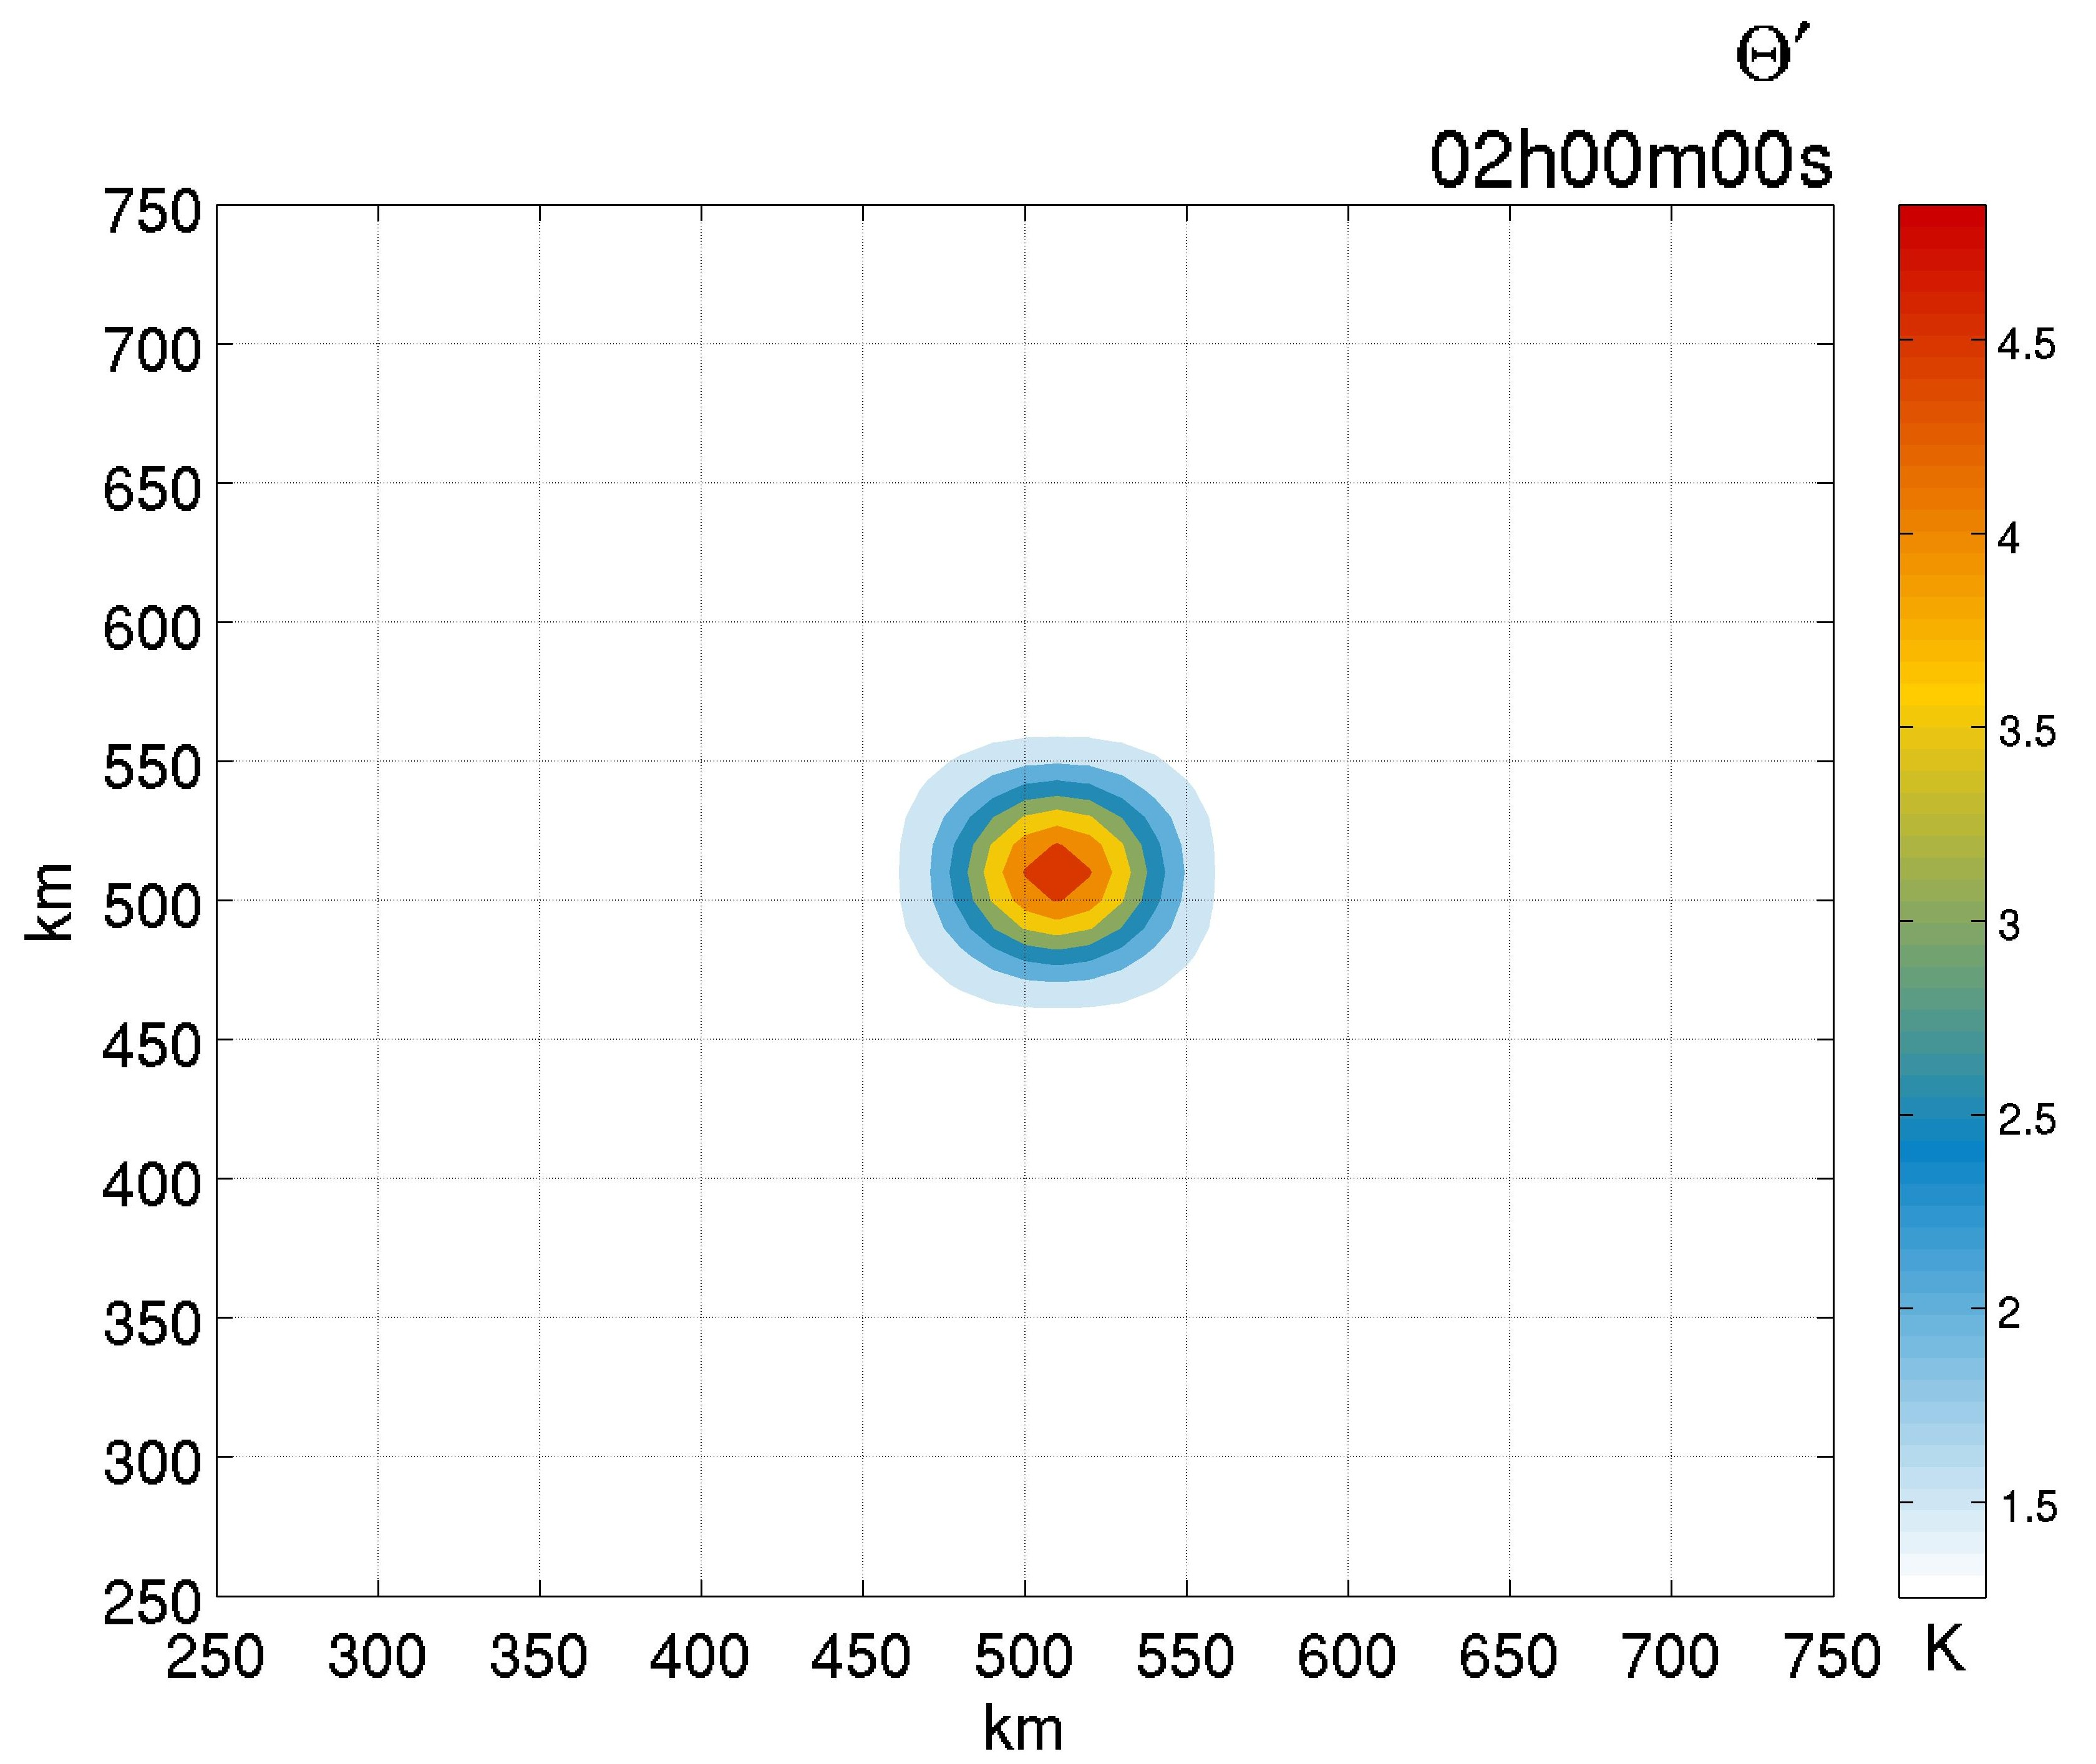
\includegraphics[width=\linewidth]{{./chapters/figures_results/ctrl_fields/pt_dev_z.x26-x76.y26-y76.ilev01.020000}.jpg}
\end{center}
\caption{Поле отклонений температуры ($\theta'$) при инициализации возмущения (2 ч. модельного времени)}
\label{fig:initanom}
\end{wrapfigure}

Влияние остальных факторов на динамику мезоциклона рассматривается с точки зрения таких интегральных характеристик, как кинетическая энергия, максимальная завихренность, минимальное приземное давление. Для интерпретации различий в результатах оценочных экспериментов привлекается анализ пространственной структуры метеополей.

Полярный мезоциклон в каждом эксперименте развивался с разной скоростью, и продолжительность экспериментов составляет 1--3 сут. Трехмерные поля в каждый момент времени интерполируются на регулярную сетку с горизонтальным разрешением, соответствующим разрешению модели. В экспериментах без фонового потока горизонтальные разрезы сфокусированы на район развития вихря (обычно $200\times 200\km$ в центре области). По вертикали данные интерполируются на регулярную сетку с шагом $500\m$ для удобства последующего постпроцессинга. В некоторых экспериментах также используется интерполяция на изобарические поверхности от $1000$ до $250\hpa$ с шагом $50\hpa$.

\section{Контрольный эксперимент}
\subsection{Начальная стадия развития вихря}
Начнем с рассмотрения момента инициализации температурной аномалии. Ее форма и начальная амплитуда видна на рис. \ref{fig:initanom}.

\begin{wrapfigure}{R}{0.5\textwidth}
\begin{center}
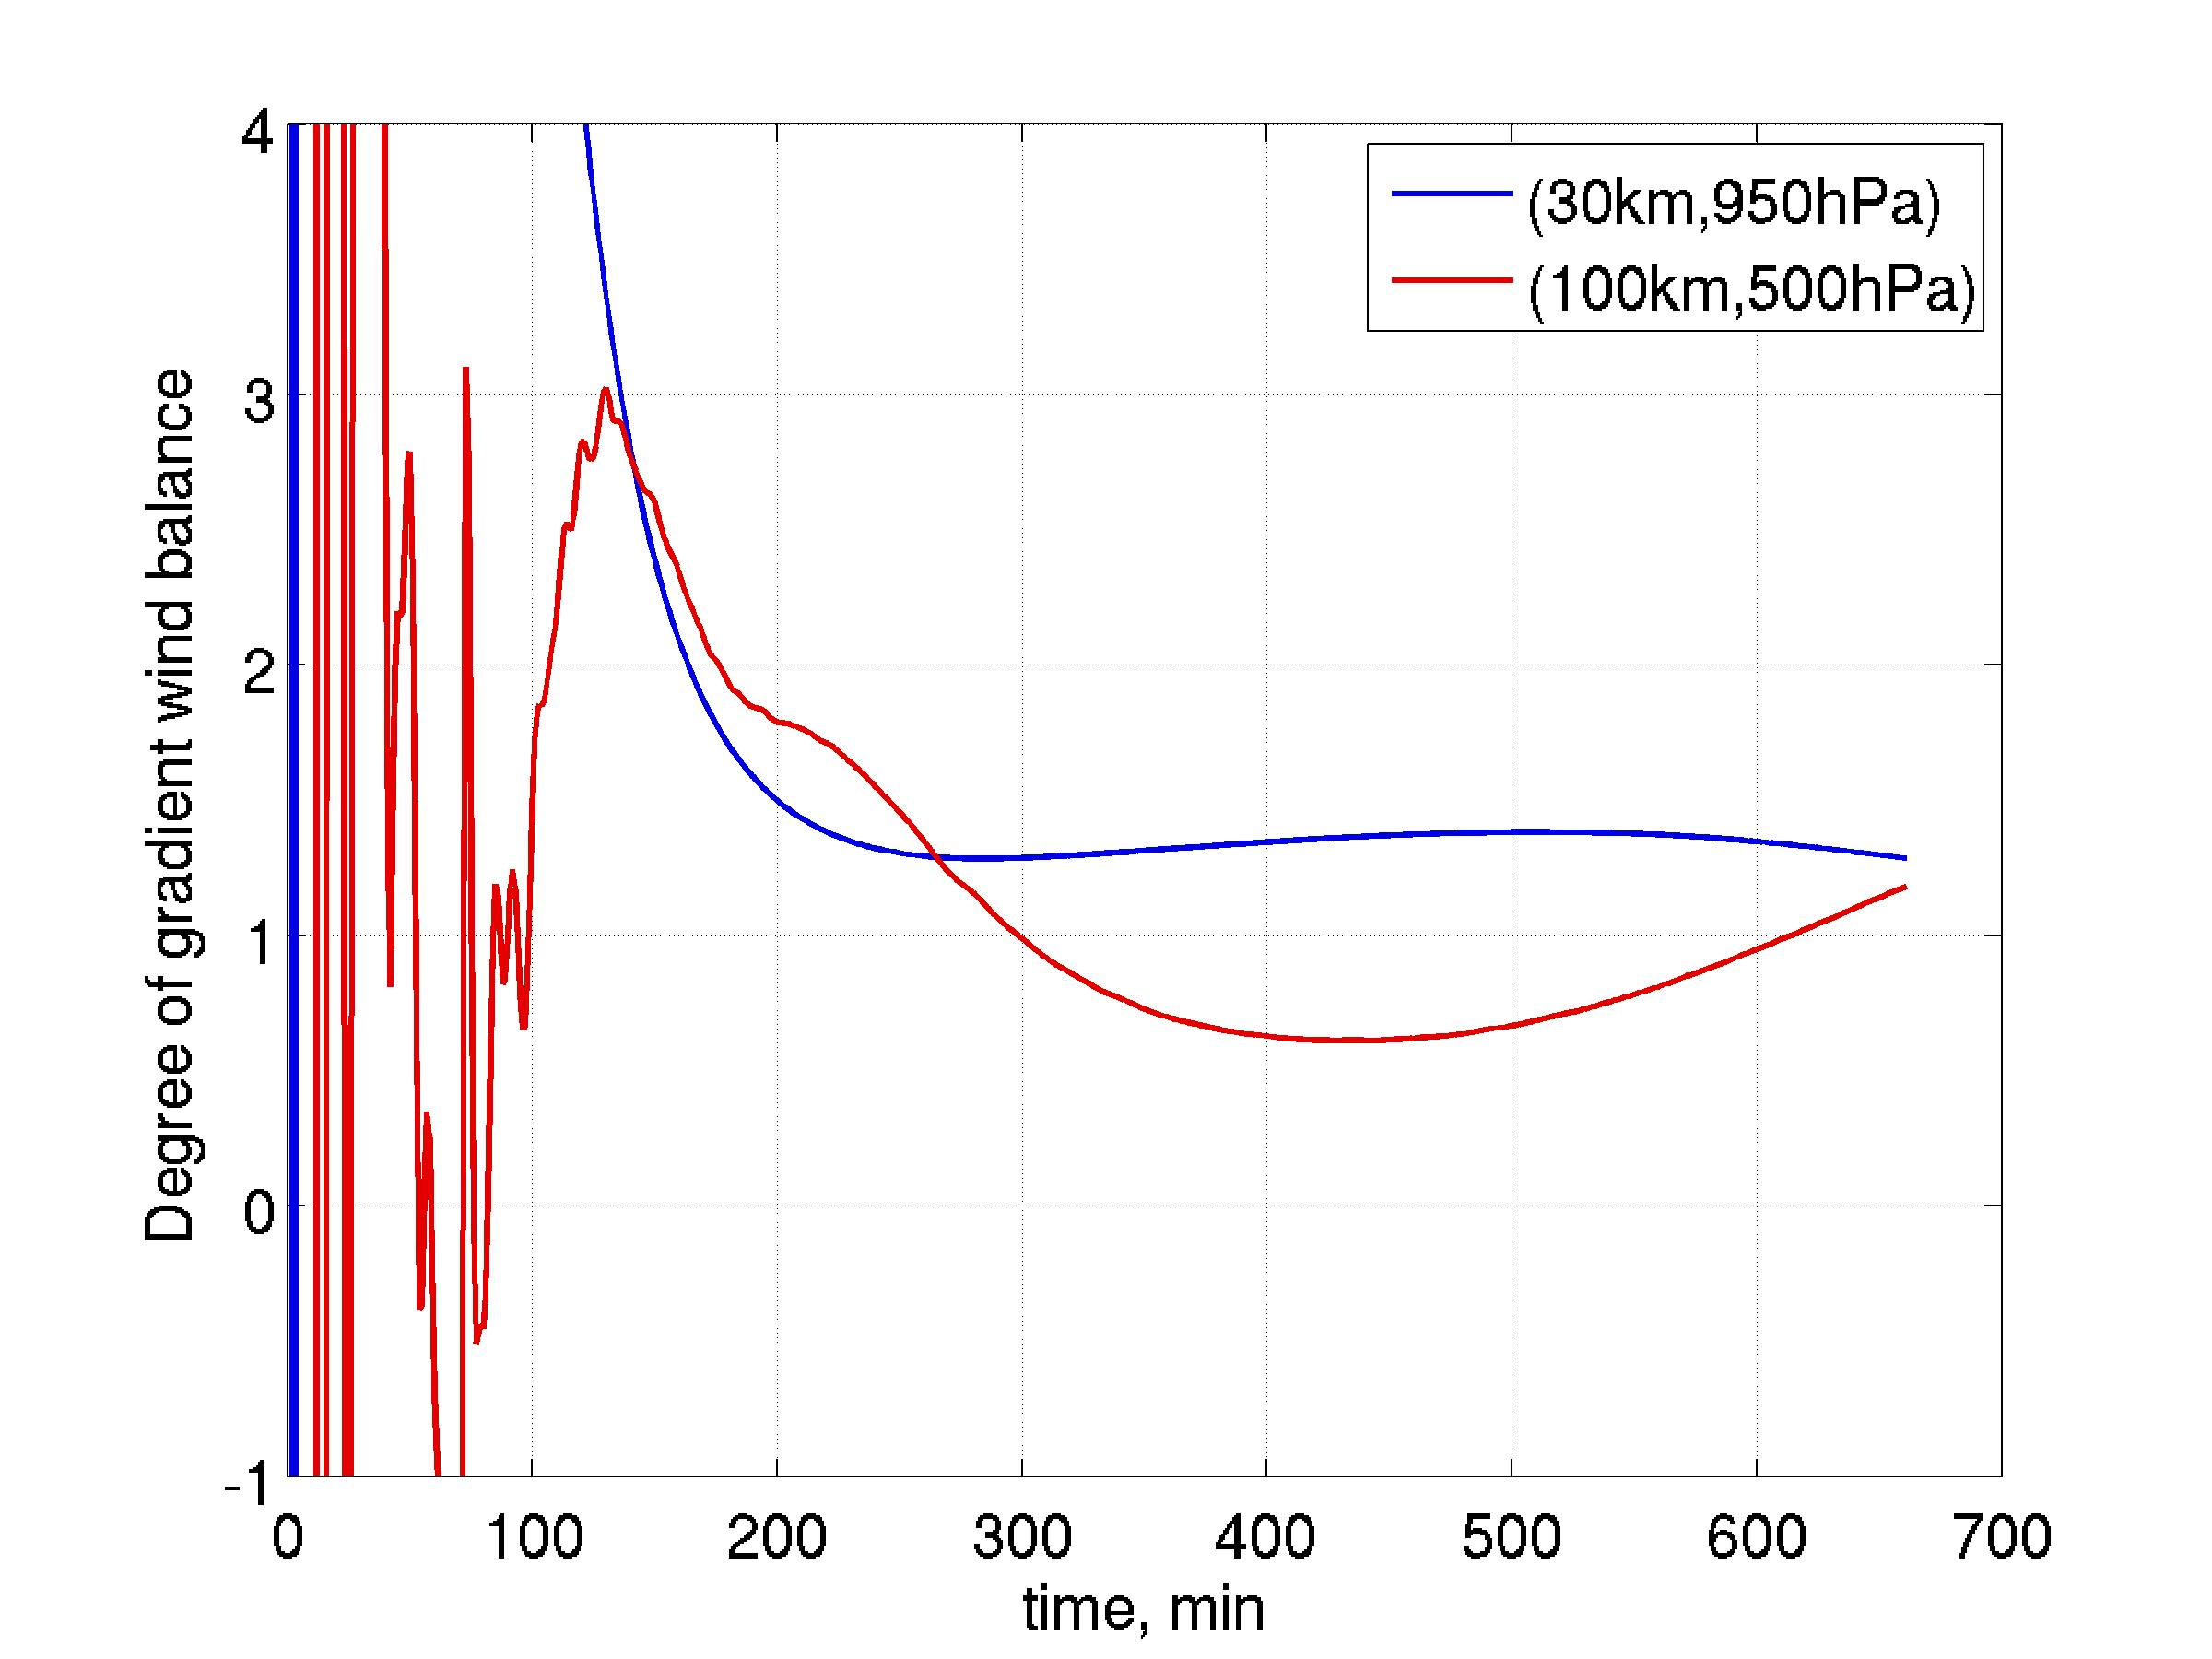
\includegraphics[width=\linewidth]{{./chapters/figures_results/ctrl_grwindbal2p}.jpg}
\end{center}
\caption{Величина градиентного баланса $\pderiv{\phi'}{r}/\left(v^2_t/r+fv_t\right)$ как функция времени с момента инициализации возмущения: при $r=30\km, p=950\hpa$ (синяя кривая) и при $r=100\km, p=500\hpa$ (красная кривая). Градиентный баланс достигается, когда кривые приближаются к $1$.}
\label{fig:grwindbal}
\end{wrapfigure} 

Появление источника тепла в атмосфере, находящейся в равновесии, ставит проблему реакции атмосферы и достижения нового баланса через механизм приспособления. Этот вопрос впервые был развит Лэмбом \citep{RT2003}, который изучал особенности волн, излучаемых в процессе гидростатического приспособления. Позднее эта проблема была обобщена как ответ устойчиво стратифицированной атмосферы на вертикально ограниченный, но горизонтально однородный источник тепла. Один из интересных результатов, полученных в работе \citep{Bannon1995}, заключаются в том, что если источник тепла горизонтально однороден, то слои воздуха ниже источника не смещаются относительно начального положения. Слои же воздуха выше источника одинаково подняты вверх. Источник нагрева в нижней тропосфере влияет на распределение давления во всей толще атмосферы выше него. Для оценки высоты, на которую распространяется влияние нагрева снизу в работе \citep{Bannon1995} было введено понятие вертикальный масштаб возмущения применительно к изотермической атмосфере. При этом в атмосфере с реалистичной структурой этот масштаб несильно отличается от такового для изотермической атмосферы. Так как распределение давления больше всего меняется на верхней границе нагретого слоя, и ответ поля давления на источник тепла убывает с высотой экспоненциально, в случае нагрева нижних слоев тропосферы эффект будет проявляться главным образом в тропосфере.

Более интересно для реальной атмосферы рассмотреть проблему Лэмба для случая неоднородного источника тепла. Например, если взять источник тепла определенного радиуса, то он будет излучать не только вертикально распространяющийся горизонтальный волновой фронт, но и сферический волновой фронт, распространяющийся от внешнего радиуса аномалии горизонтально и вертикально. 

Подобный процесс наблюдается в начале каждого эксперимента данной работы. Ввиду того, что нагрев в районе аномалии происходит не мгновенно, а в течение конечного отрезка времени, как и бывает в реальной атмосфере,  фронт излучаемых волн прослеживается слабее. Тем не менее, результат качественно совпадает идеализированными экспериментами \citep{RT2003}. Вертикальный барический градиент находится почти в гидростатическом балансе с силой плавучести, а горизонтальный создает циклоническую циркуляцию. Такая циркуляция возникает в устойчиво стратифицированной атмосфере, и источник энергии в виде конвективной доступной потенциальной энергии (CAPE) не является необходимым. При остановке подачи тепла не вращающаяся атмосфера постепенно придет к состоянию покоя. Однако это не так, если атмосфера испытывает вращение, что подтверждается в наших экспериментах \ref{sec:res:nohle}.

\begin{wrapfigure}{L}{0.5\textwidth}
\centering
\vspace{-20pt}
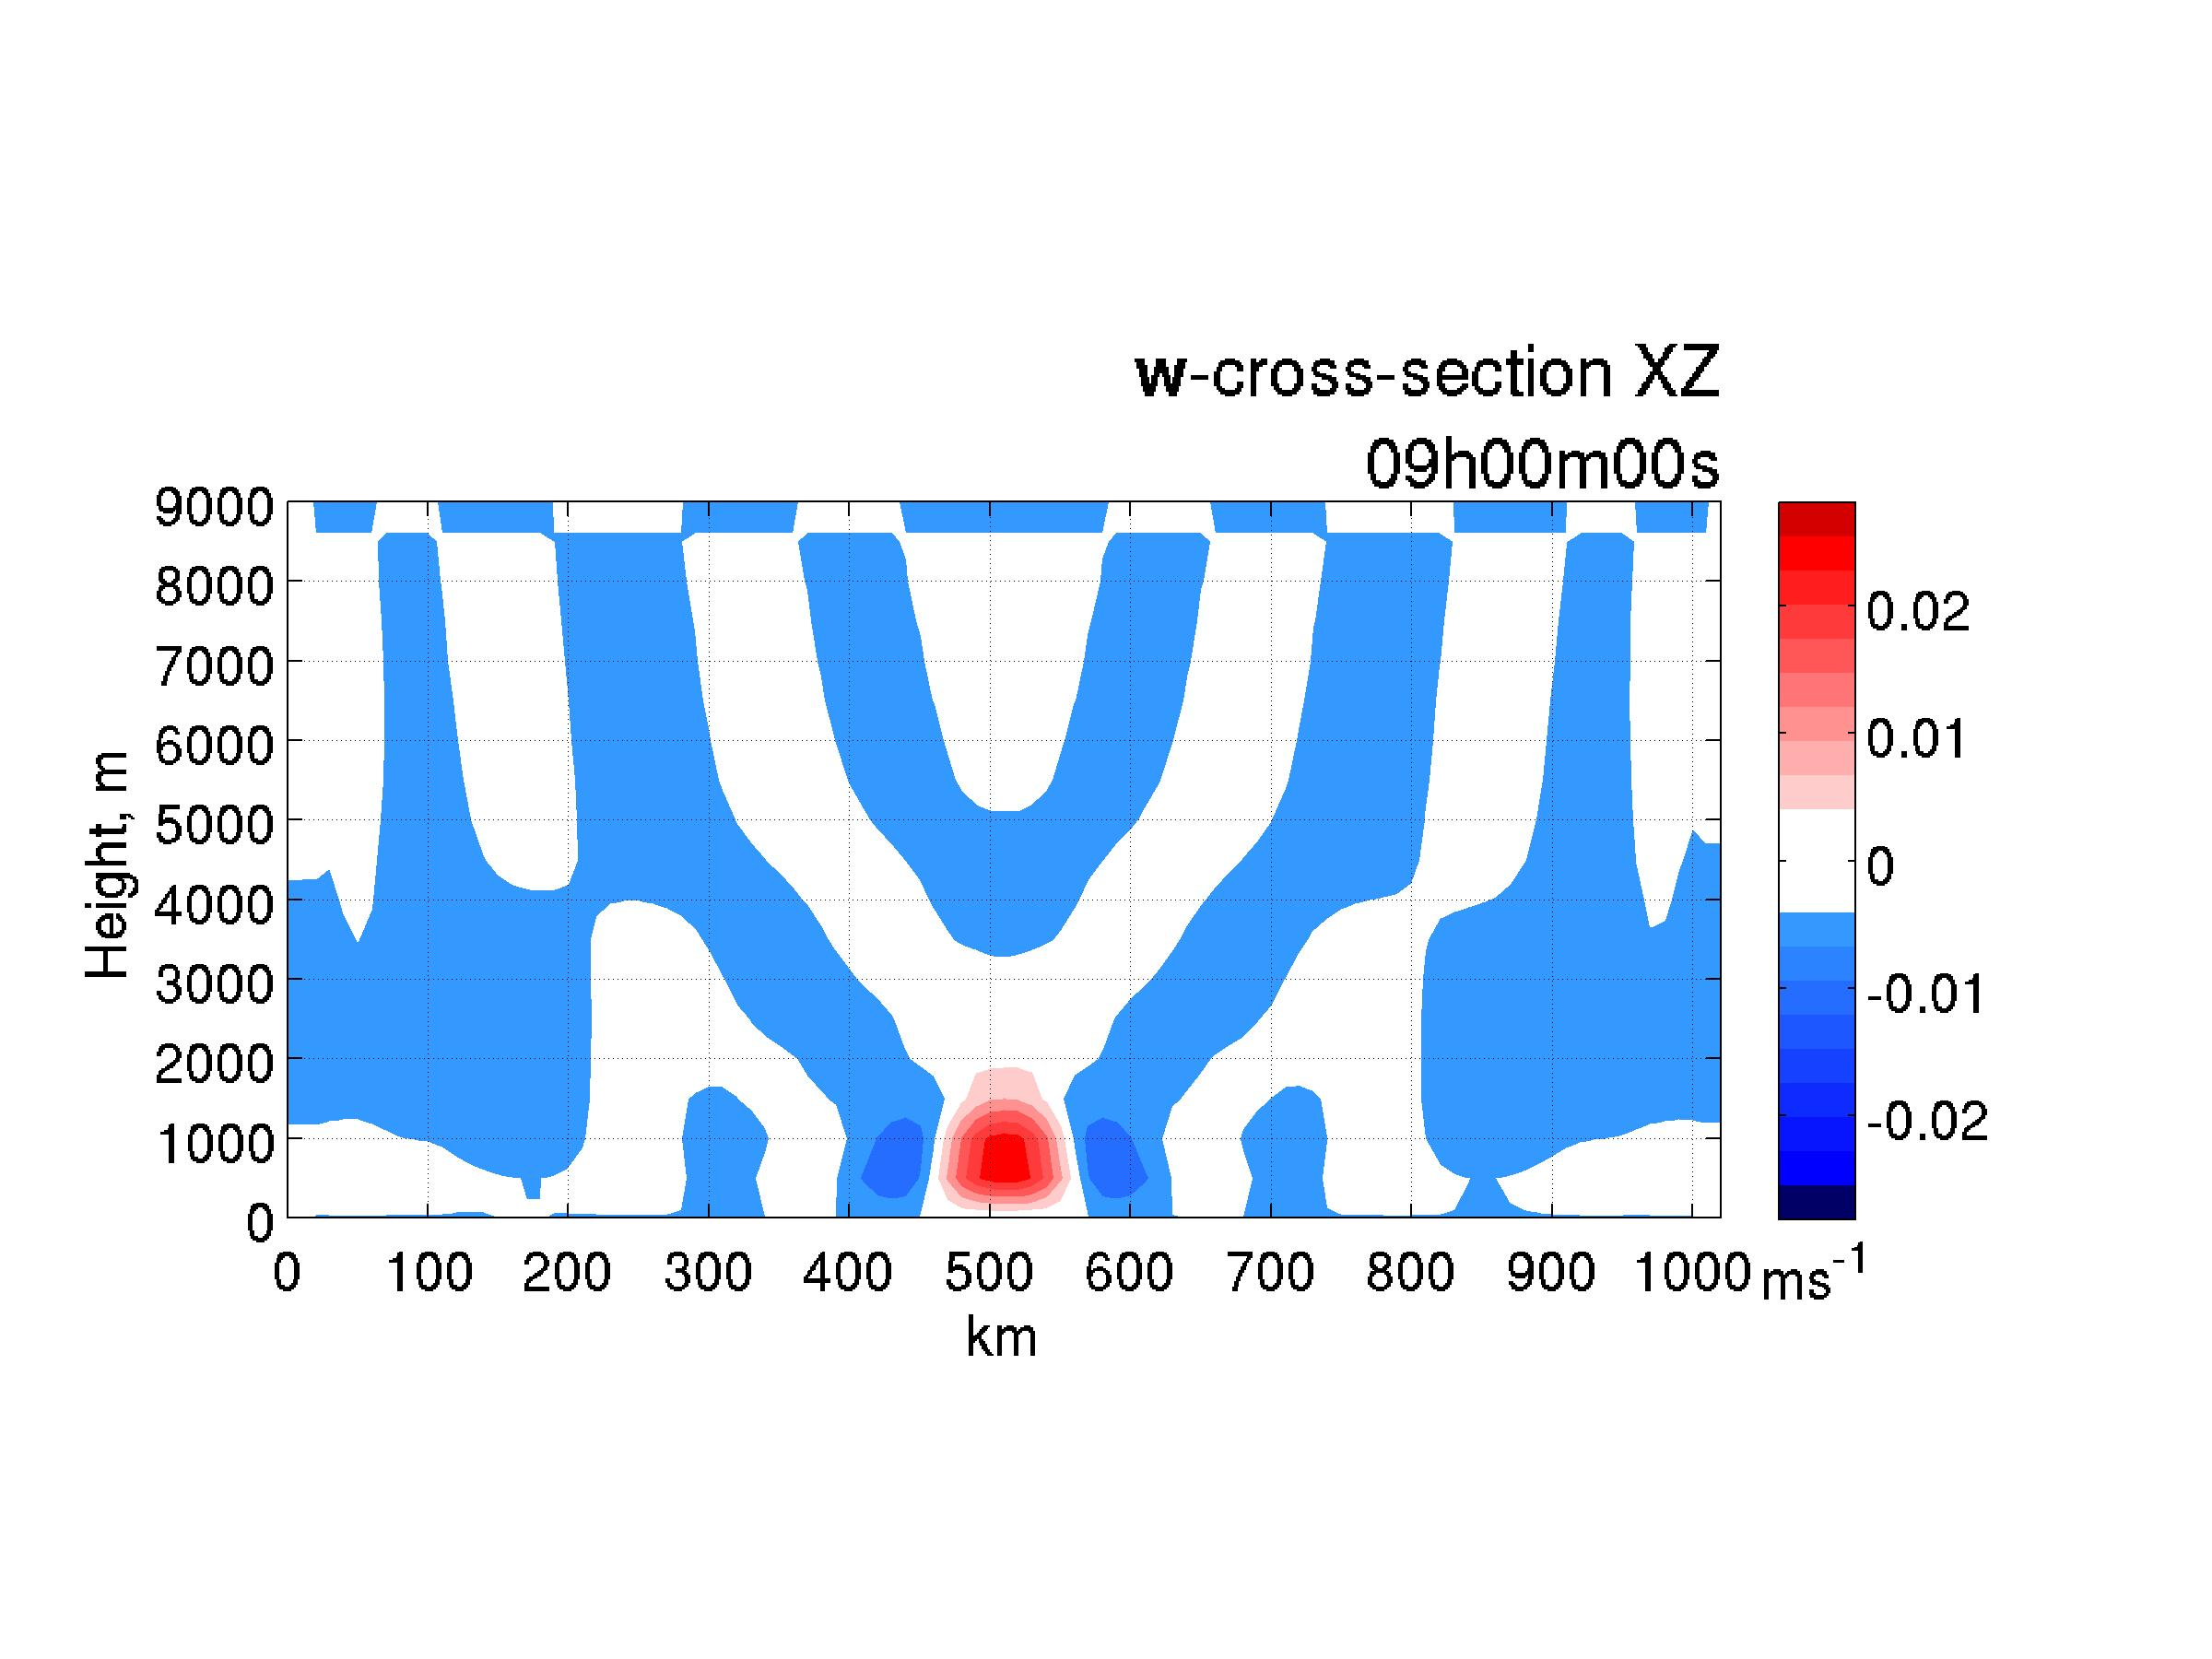
\includegraphics[width=\linewidth]{{./chapters/figures_results/ctrl_fields/W_cross_z.iy52.090000}.jpg}
\vspace{-10pt}
\caption{Меридиональный разрез вертикальной скорости $w$. Эксперимент CTRL. 9 час модельного времени.}
\label{fig:wcross}
\end{wrapfigure} 

Начальная куполообразная аномалия приводит к возникновению в нижних слоях атмосферы горизонтального градиента давления, который создает конвергенцию массы в центре области. В результате под влиянием силы Кориолиса возникают инерционно-гравитационные волны, в то время как возникновение звуковых волн невозможно ввиду разрешения сетки модели \citep{MillerWhite1984,MirandaPhD}. Путем излучения инерционно-гравитационных волн происходит приспособление атмосферы к градиентному балансу (\ref{fig:grwindbal}).

Разрез поля вертикальной скорости \ref{fig:wcross} дает представление о распространении гравитационных волн в ответ на температурное возмущение. Рисунок схож с результатами линейной теории \citep{Lin2007}, однако более правдоподобен из-за нелинейности процессов и интерференции волн в реальной атмосфере. При задании неоднородного фонового профиля стратификации области подъема и нисхождения воздуха, очевидно, будут иметь несимметричную форму.

Несмотря на четко различимые в начале моделирования волны, их влияние мало: аномалия потенциального вихря, определяющая циркуляцию в атмосфере, остается на месте, где она была изначально помещена. На рис. \ref{fig:grwindbal} частота проходящих через выбранные точки волн уменьшается, то есть волны с меньшими частотами остаются в вихре, а более высокочастотные волны распространяются наружу. Другими словами, возмущение потенциального вихря не переносится вместе с инерционно-гравитационными волнами \citep{RT2003}. Влияние волн, созданных начальным дисбалансом в атмосфере пренебрежимо мало по сравнению с 'равновесной' частью движения, которое связано через принцип обратимости с распределением потенциального вихря.

\begin{figure}[t]
	\centering
	\begin{subfigure}[t]{0.3\textwidth}
		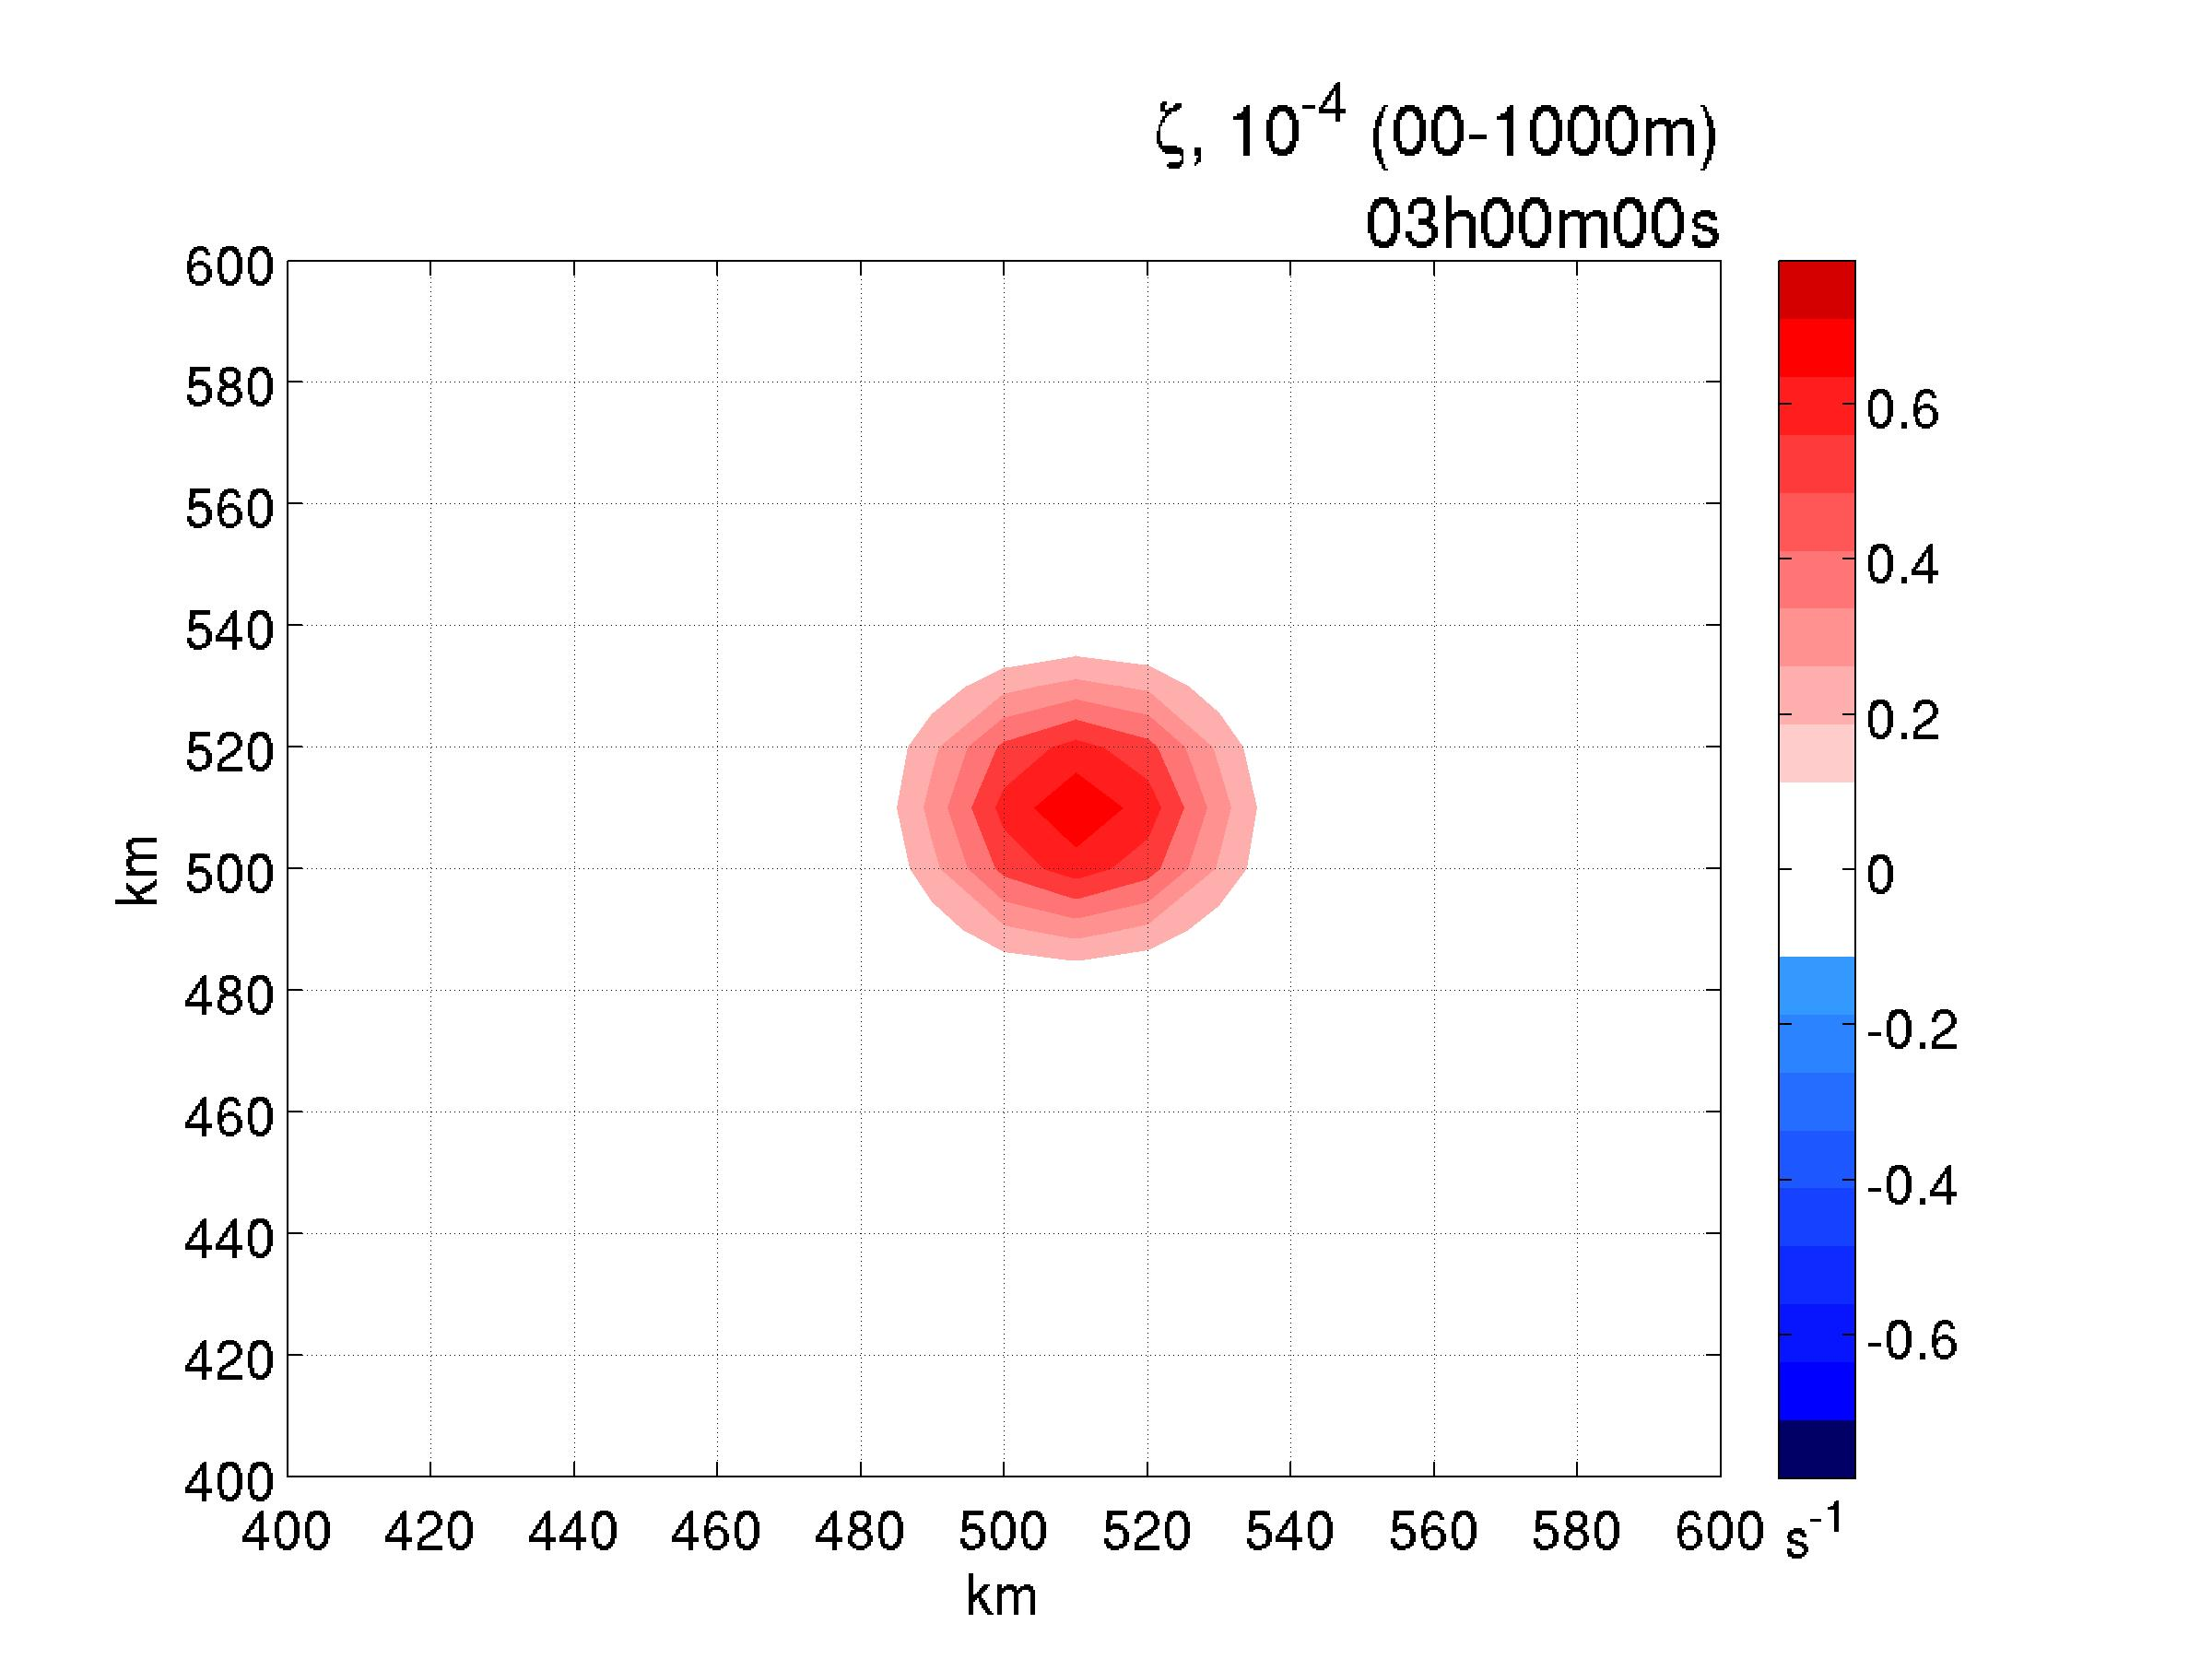
\includegraphics[width=\linewidth]{{./chapters/figures_results/ctrl_fields/rot_z_z.x41-x61.y41-y61.ilev02.030000}.jpg}
		\caption{Относительная завихренность ($\zeta$), $\pers$.}
        \label{fig:ctrl_rotz03}
	\end{subfigure}
	\hfill
	\begin{subfigure}[t]{0.3\textwidth}
		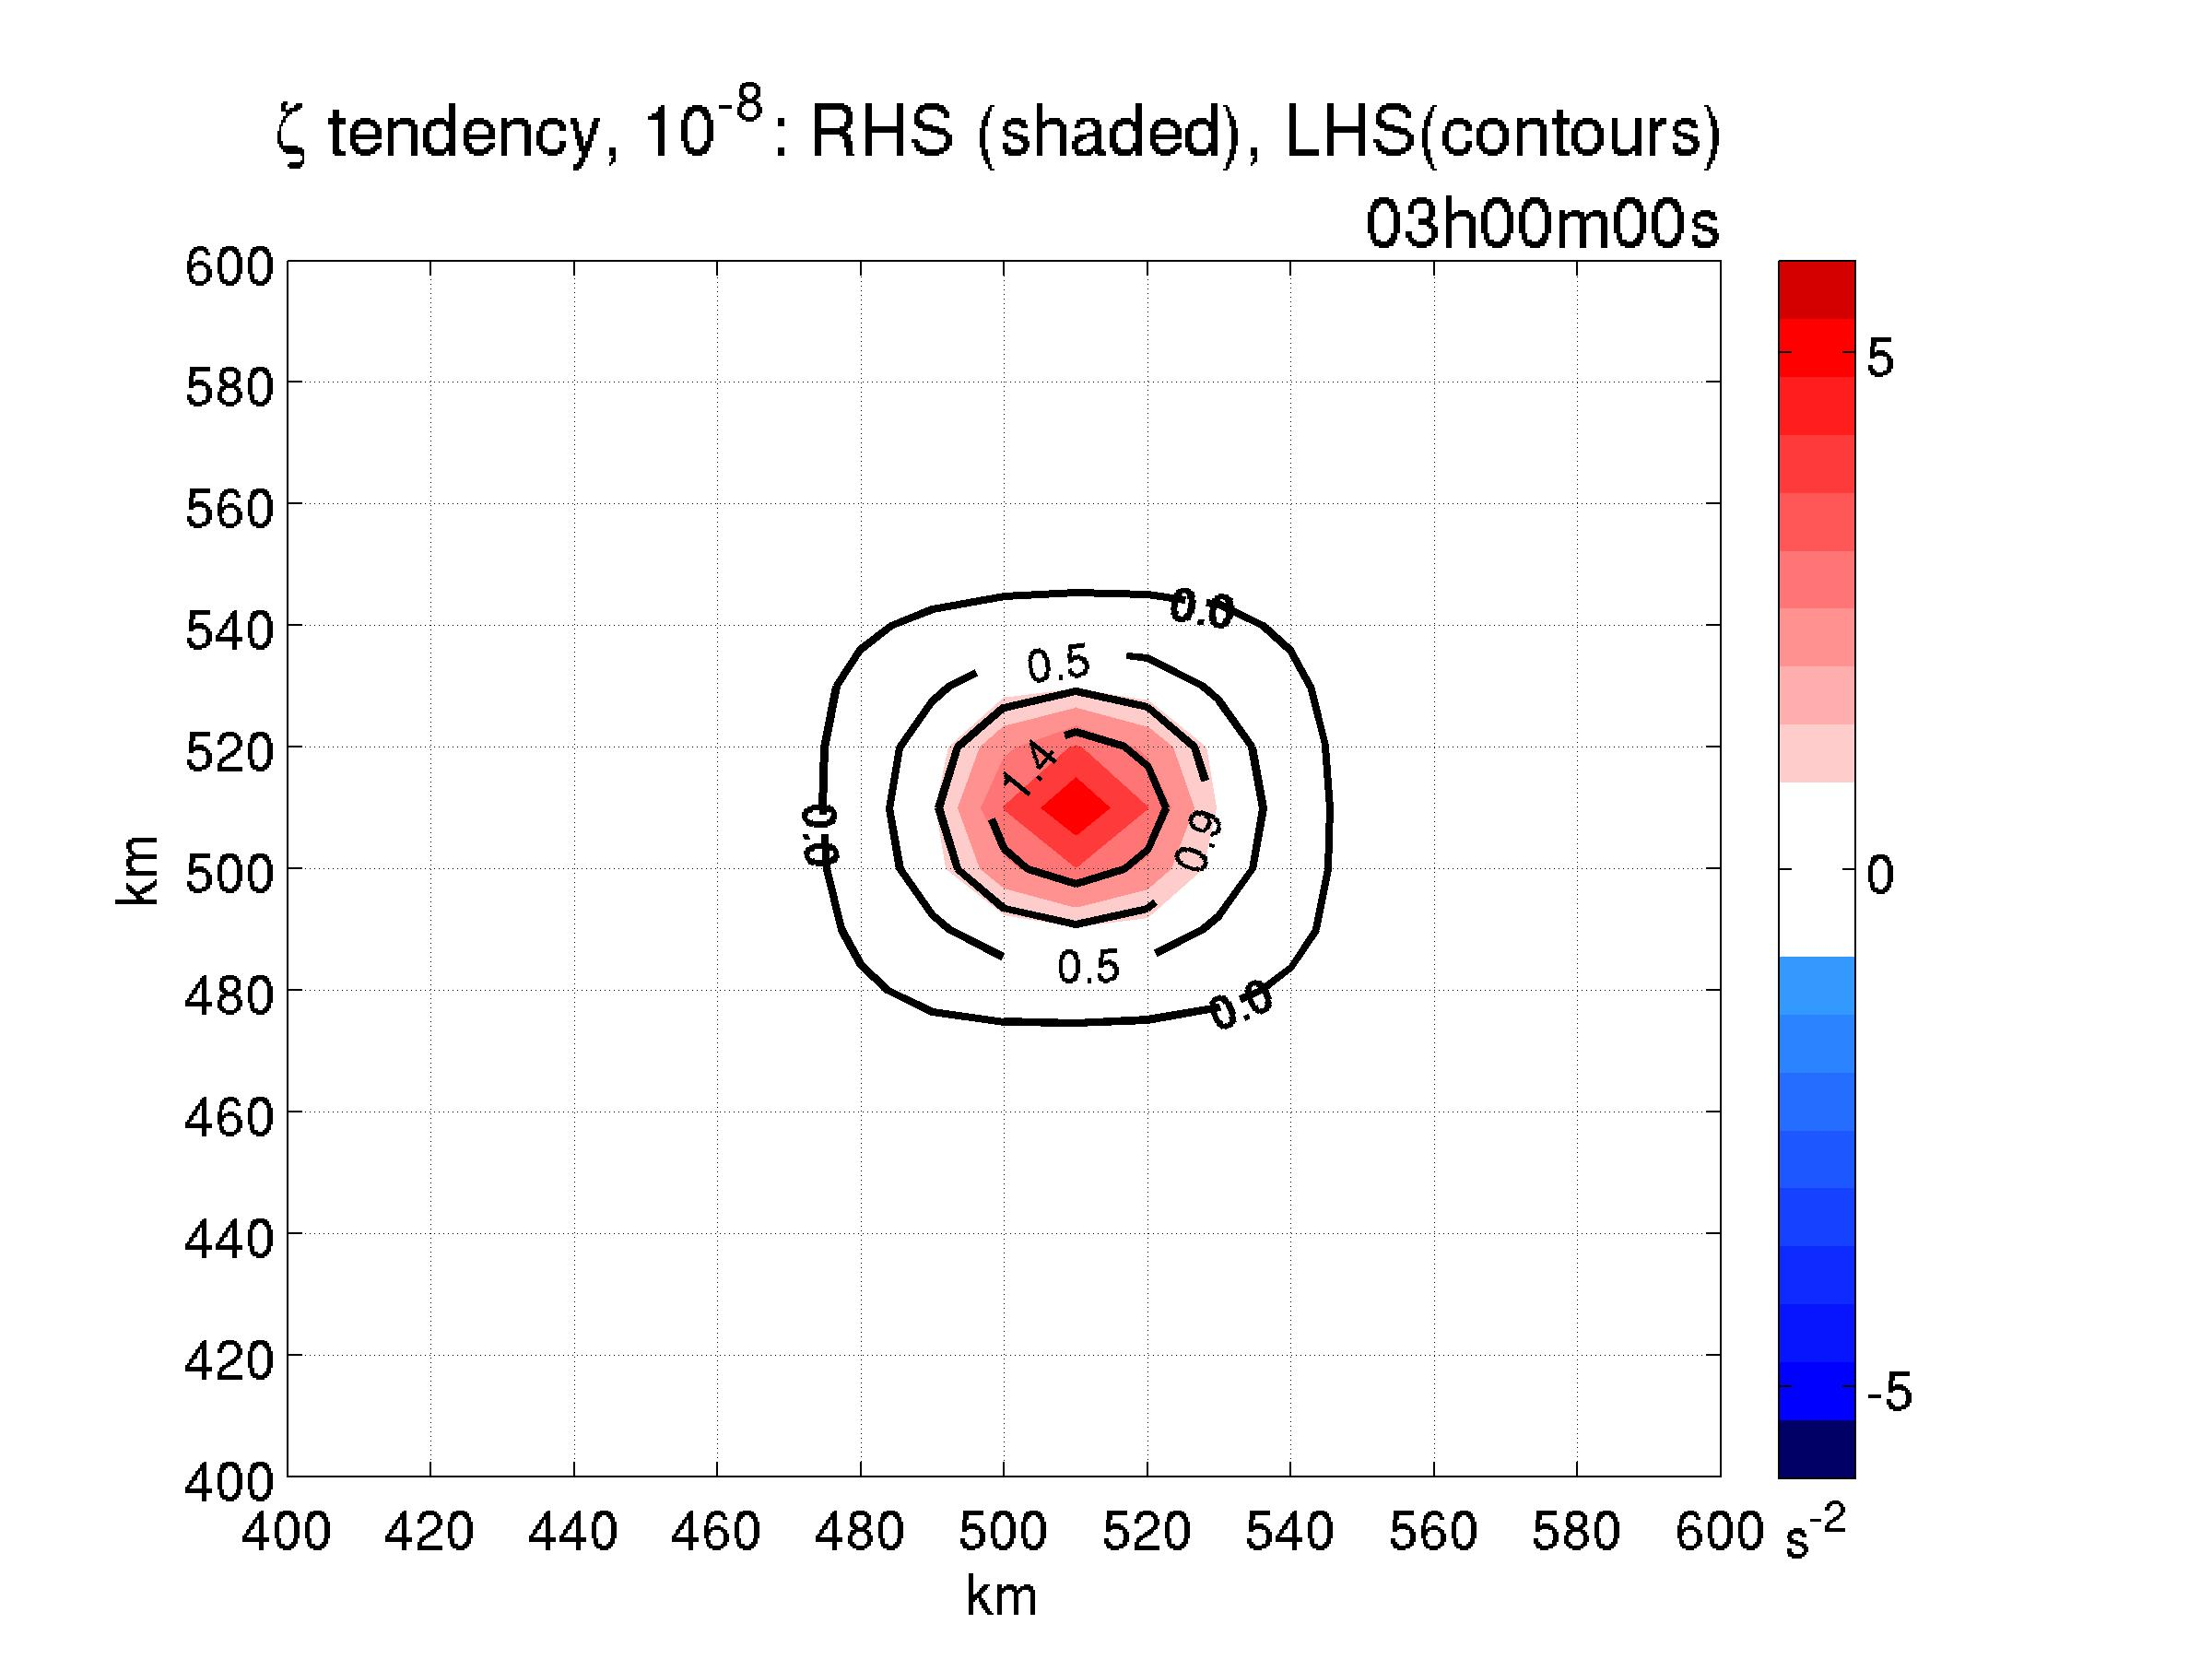
\includegraphics[width=\linewidth]{{./chapters/figures_results/ctrl_fields/vort_bud_z.x41-x61.y41-y61.ilev02.030000}.jpg}
		\caption{Тенденция относительной завихренности ($\pderiv{\zeta}{t}$), $\s^{-2}$.}
		\label{fig:ctrl_vorttend03}
	\end{subfigure}
	\hfill
    \begin{subfigure}[t]{0.3\textwidth}
		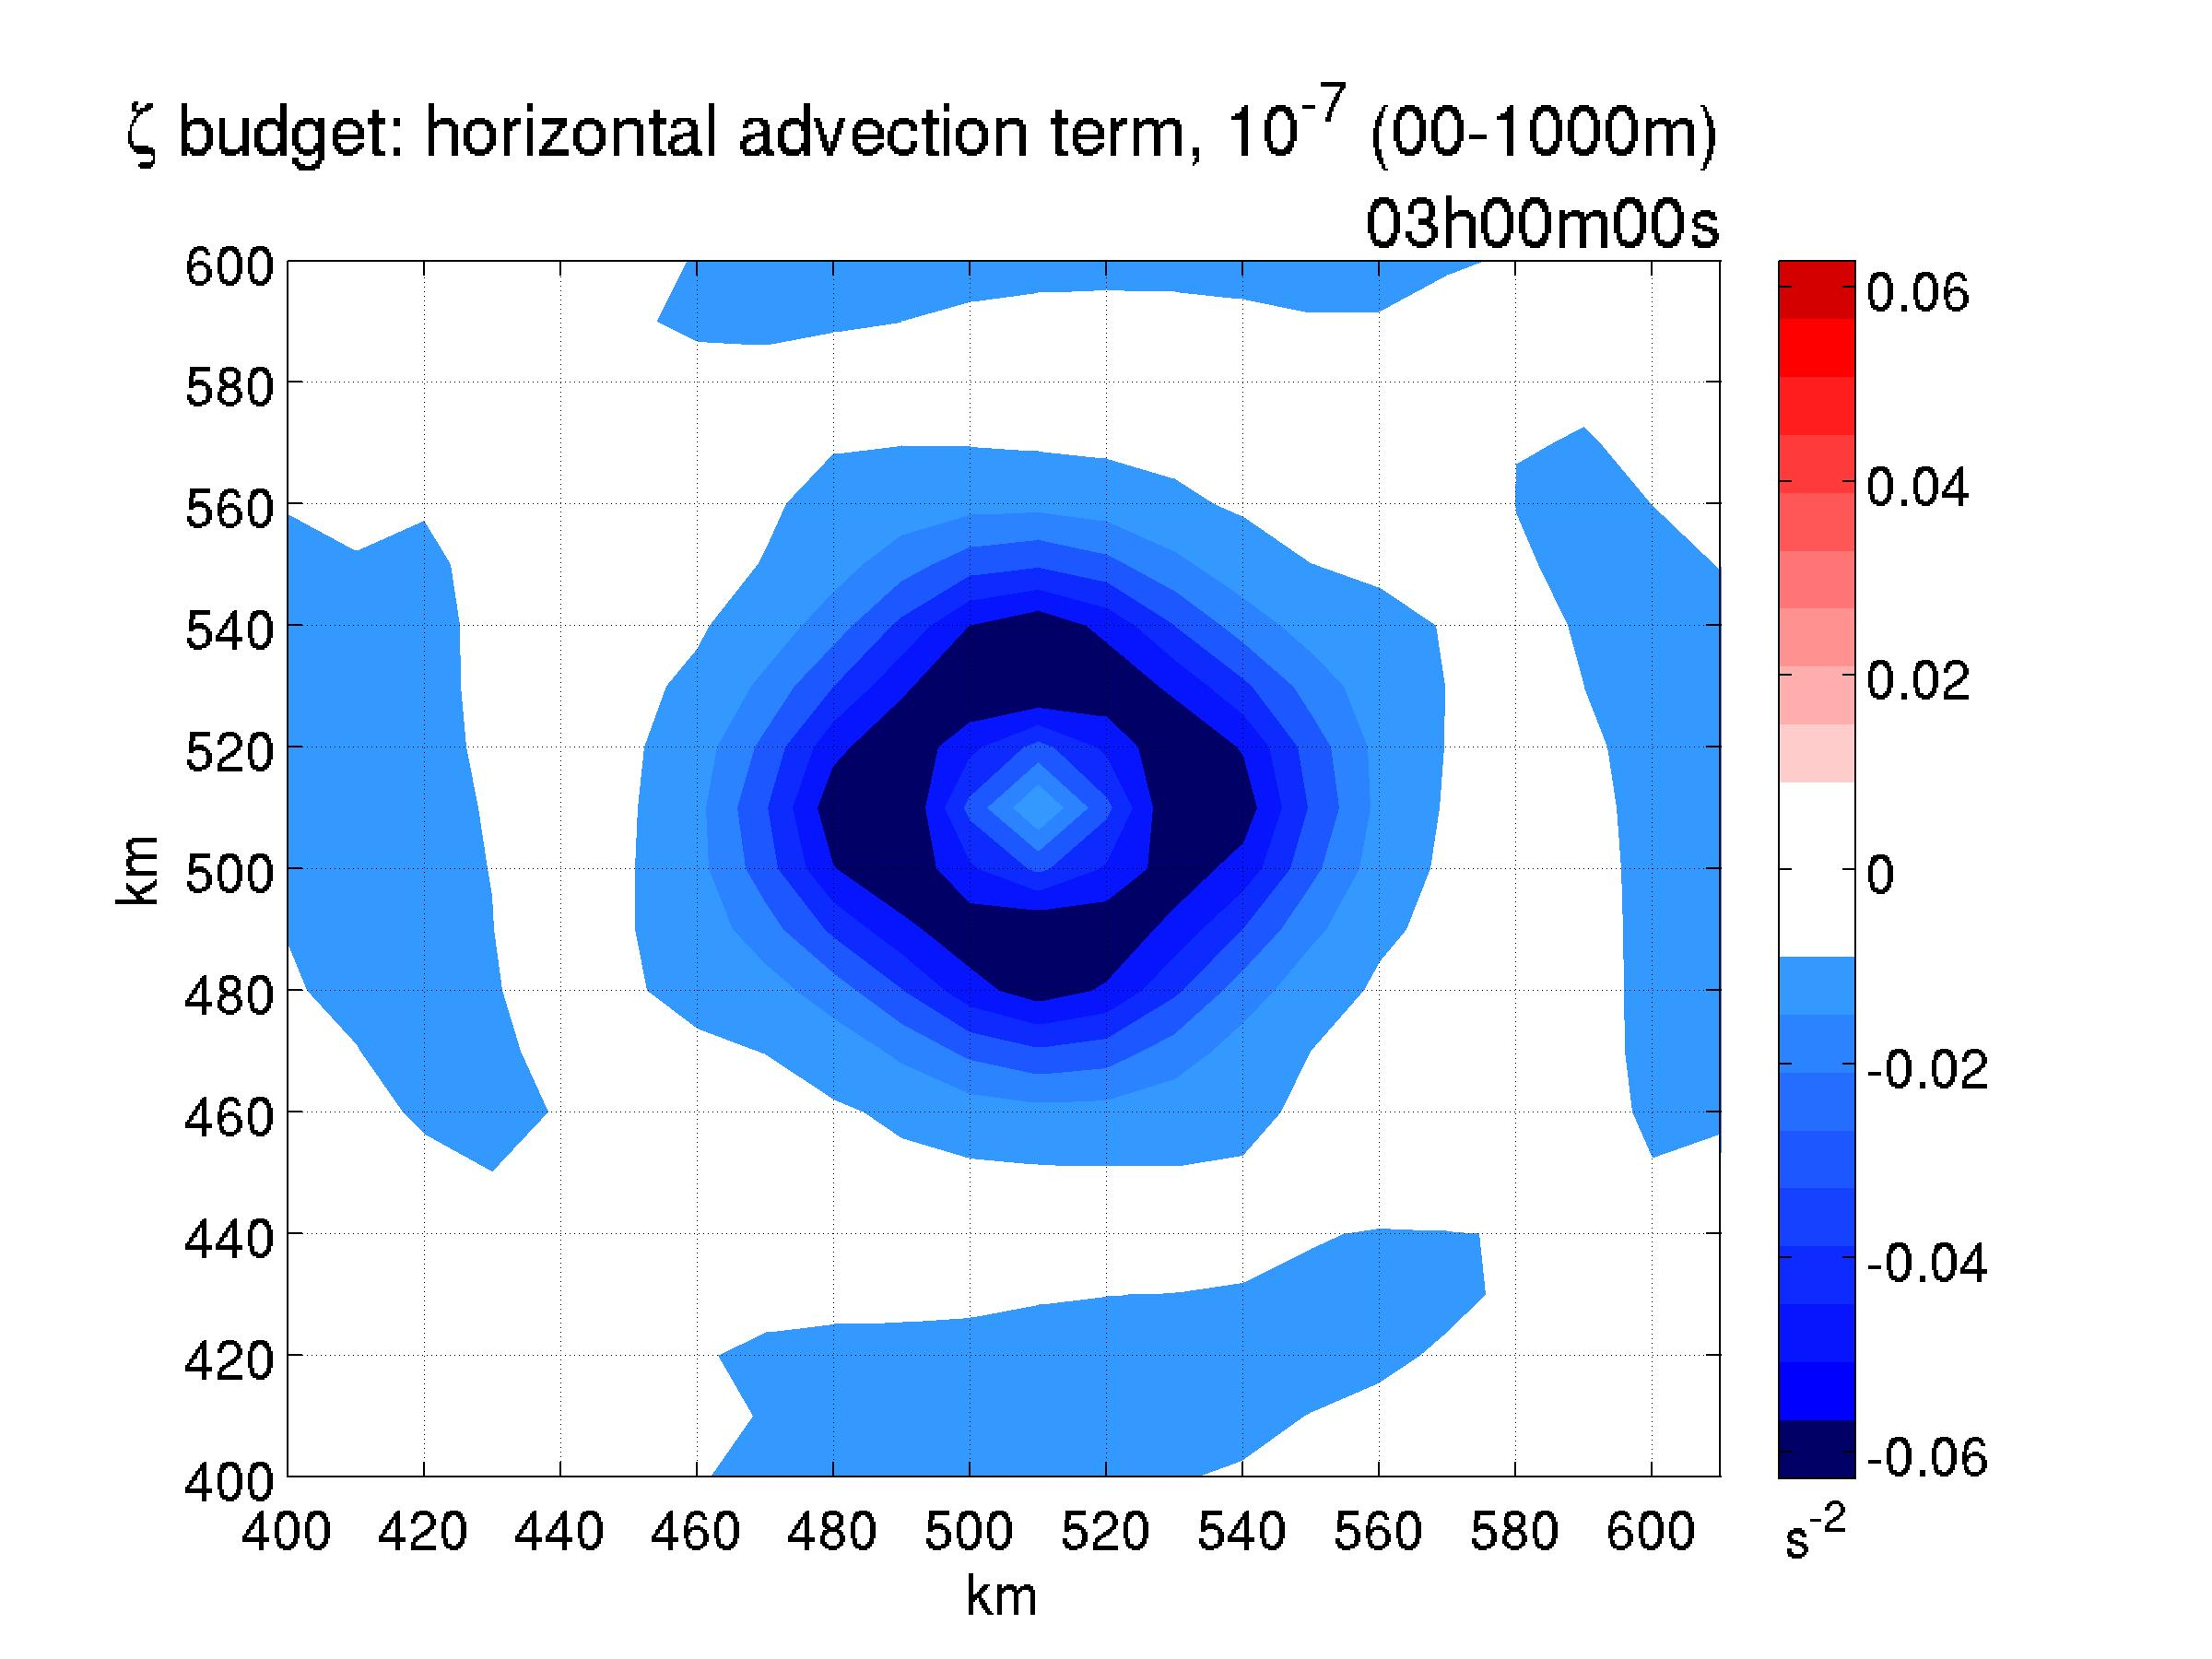
\includegraphics[width=\linewidth]{{./chapters/figures_results/ctrl_fields/vort_budget_hadv_z.x41-x62.y41-y61.ilev02.030000}.jpg}
		\caption{Слагаемое горизонтальной адвекции, $\s^{-2}$.}
		\label{fig:ctrl_hadv03}
	\end{subfigure}
	\hfill
	\begin{subfigure}[t]{0.3\textwidth}
		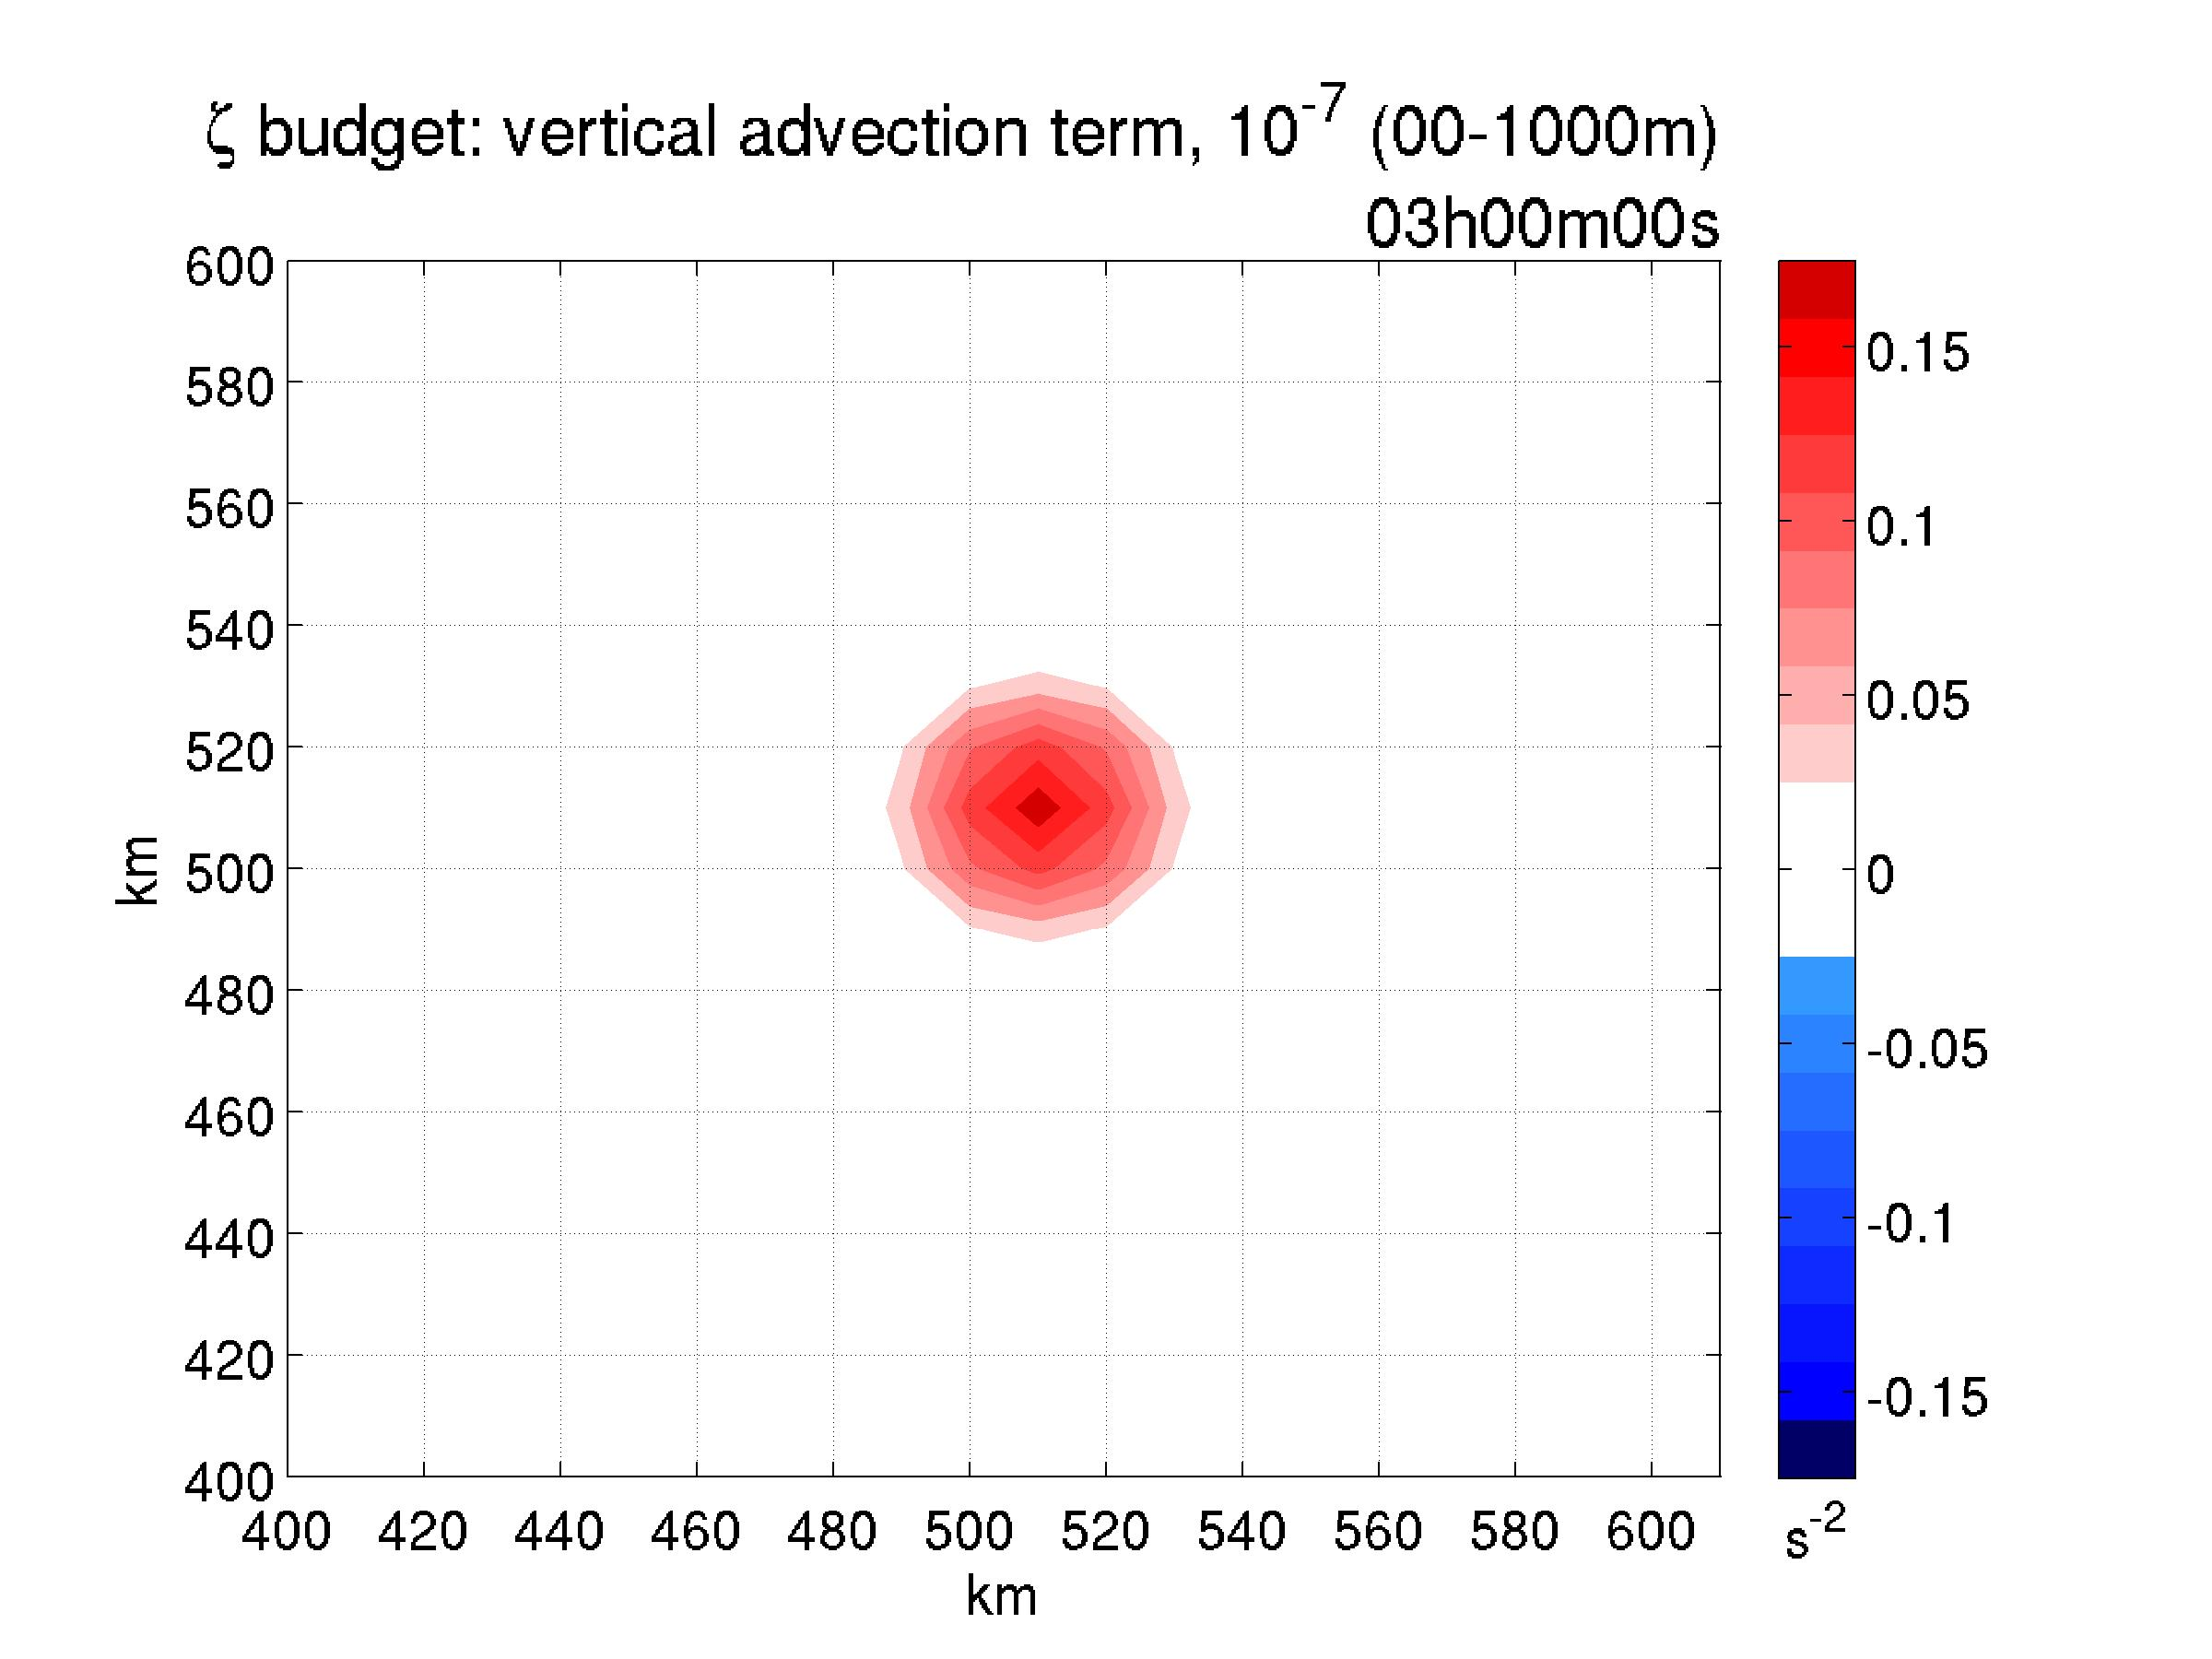
\includegraphics[width=\linewidth]{{./chapters/figures_results/ctrl_fields/vort_budget_vadv_z.x41-x62.y41-y61.ilev02.030000}.jpg}
		\caption{Слагаемое вертикальной адвекции, $\s^{-2}$.}
		\label{fig:ctrl_vadv03}
	\end{subfigure}
	\hfill
	\begin{subfigure}[t]{0.3\textwidth}
		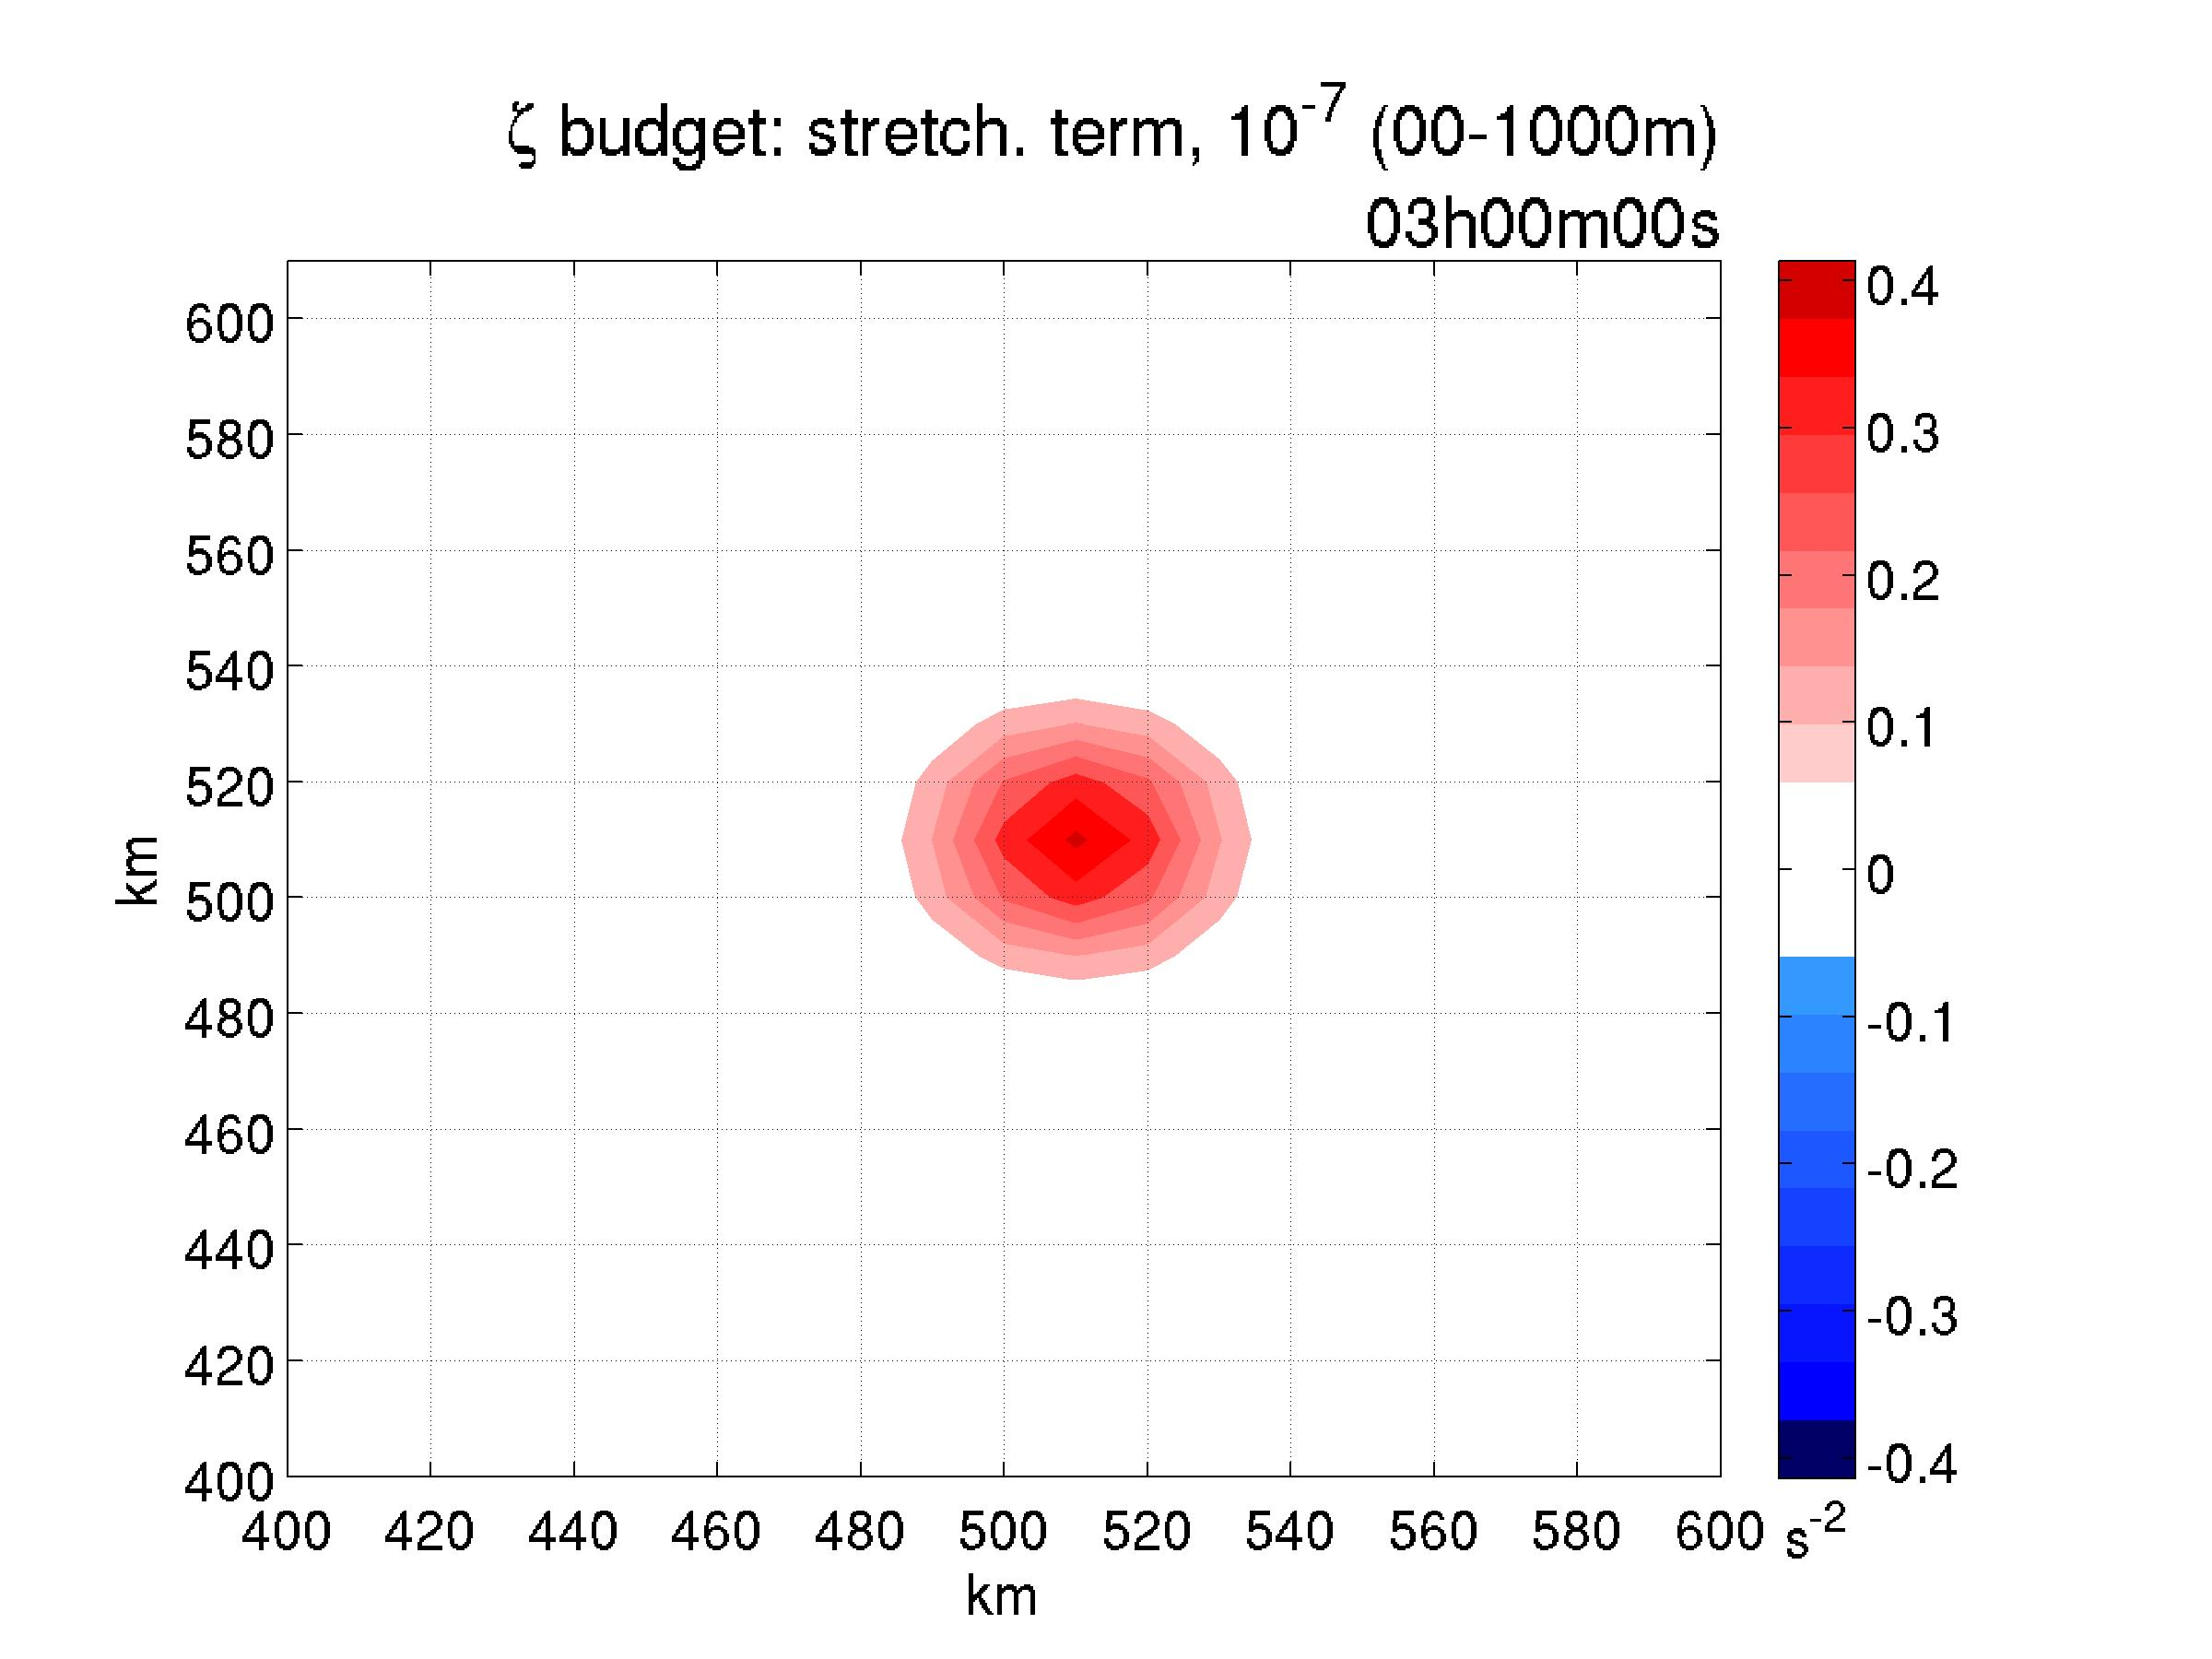
\includegraphics[width=\linewidth]{{./chapters/figures_results/ctrl_fields/vort_budget_stretch_z.x41-x62.y41-y61.ilev02.030000}.jpg}
		\caption{Слагаемое растяжения, $\s^{-2}$.}
		\label{fig:ctrl_stretch03}
	\end{subfigure}
	\hfill
	\begin{subfigure}[t]{0.3\textwidth}
		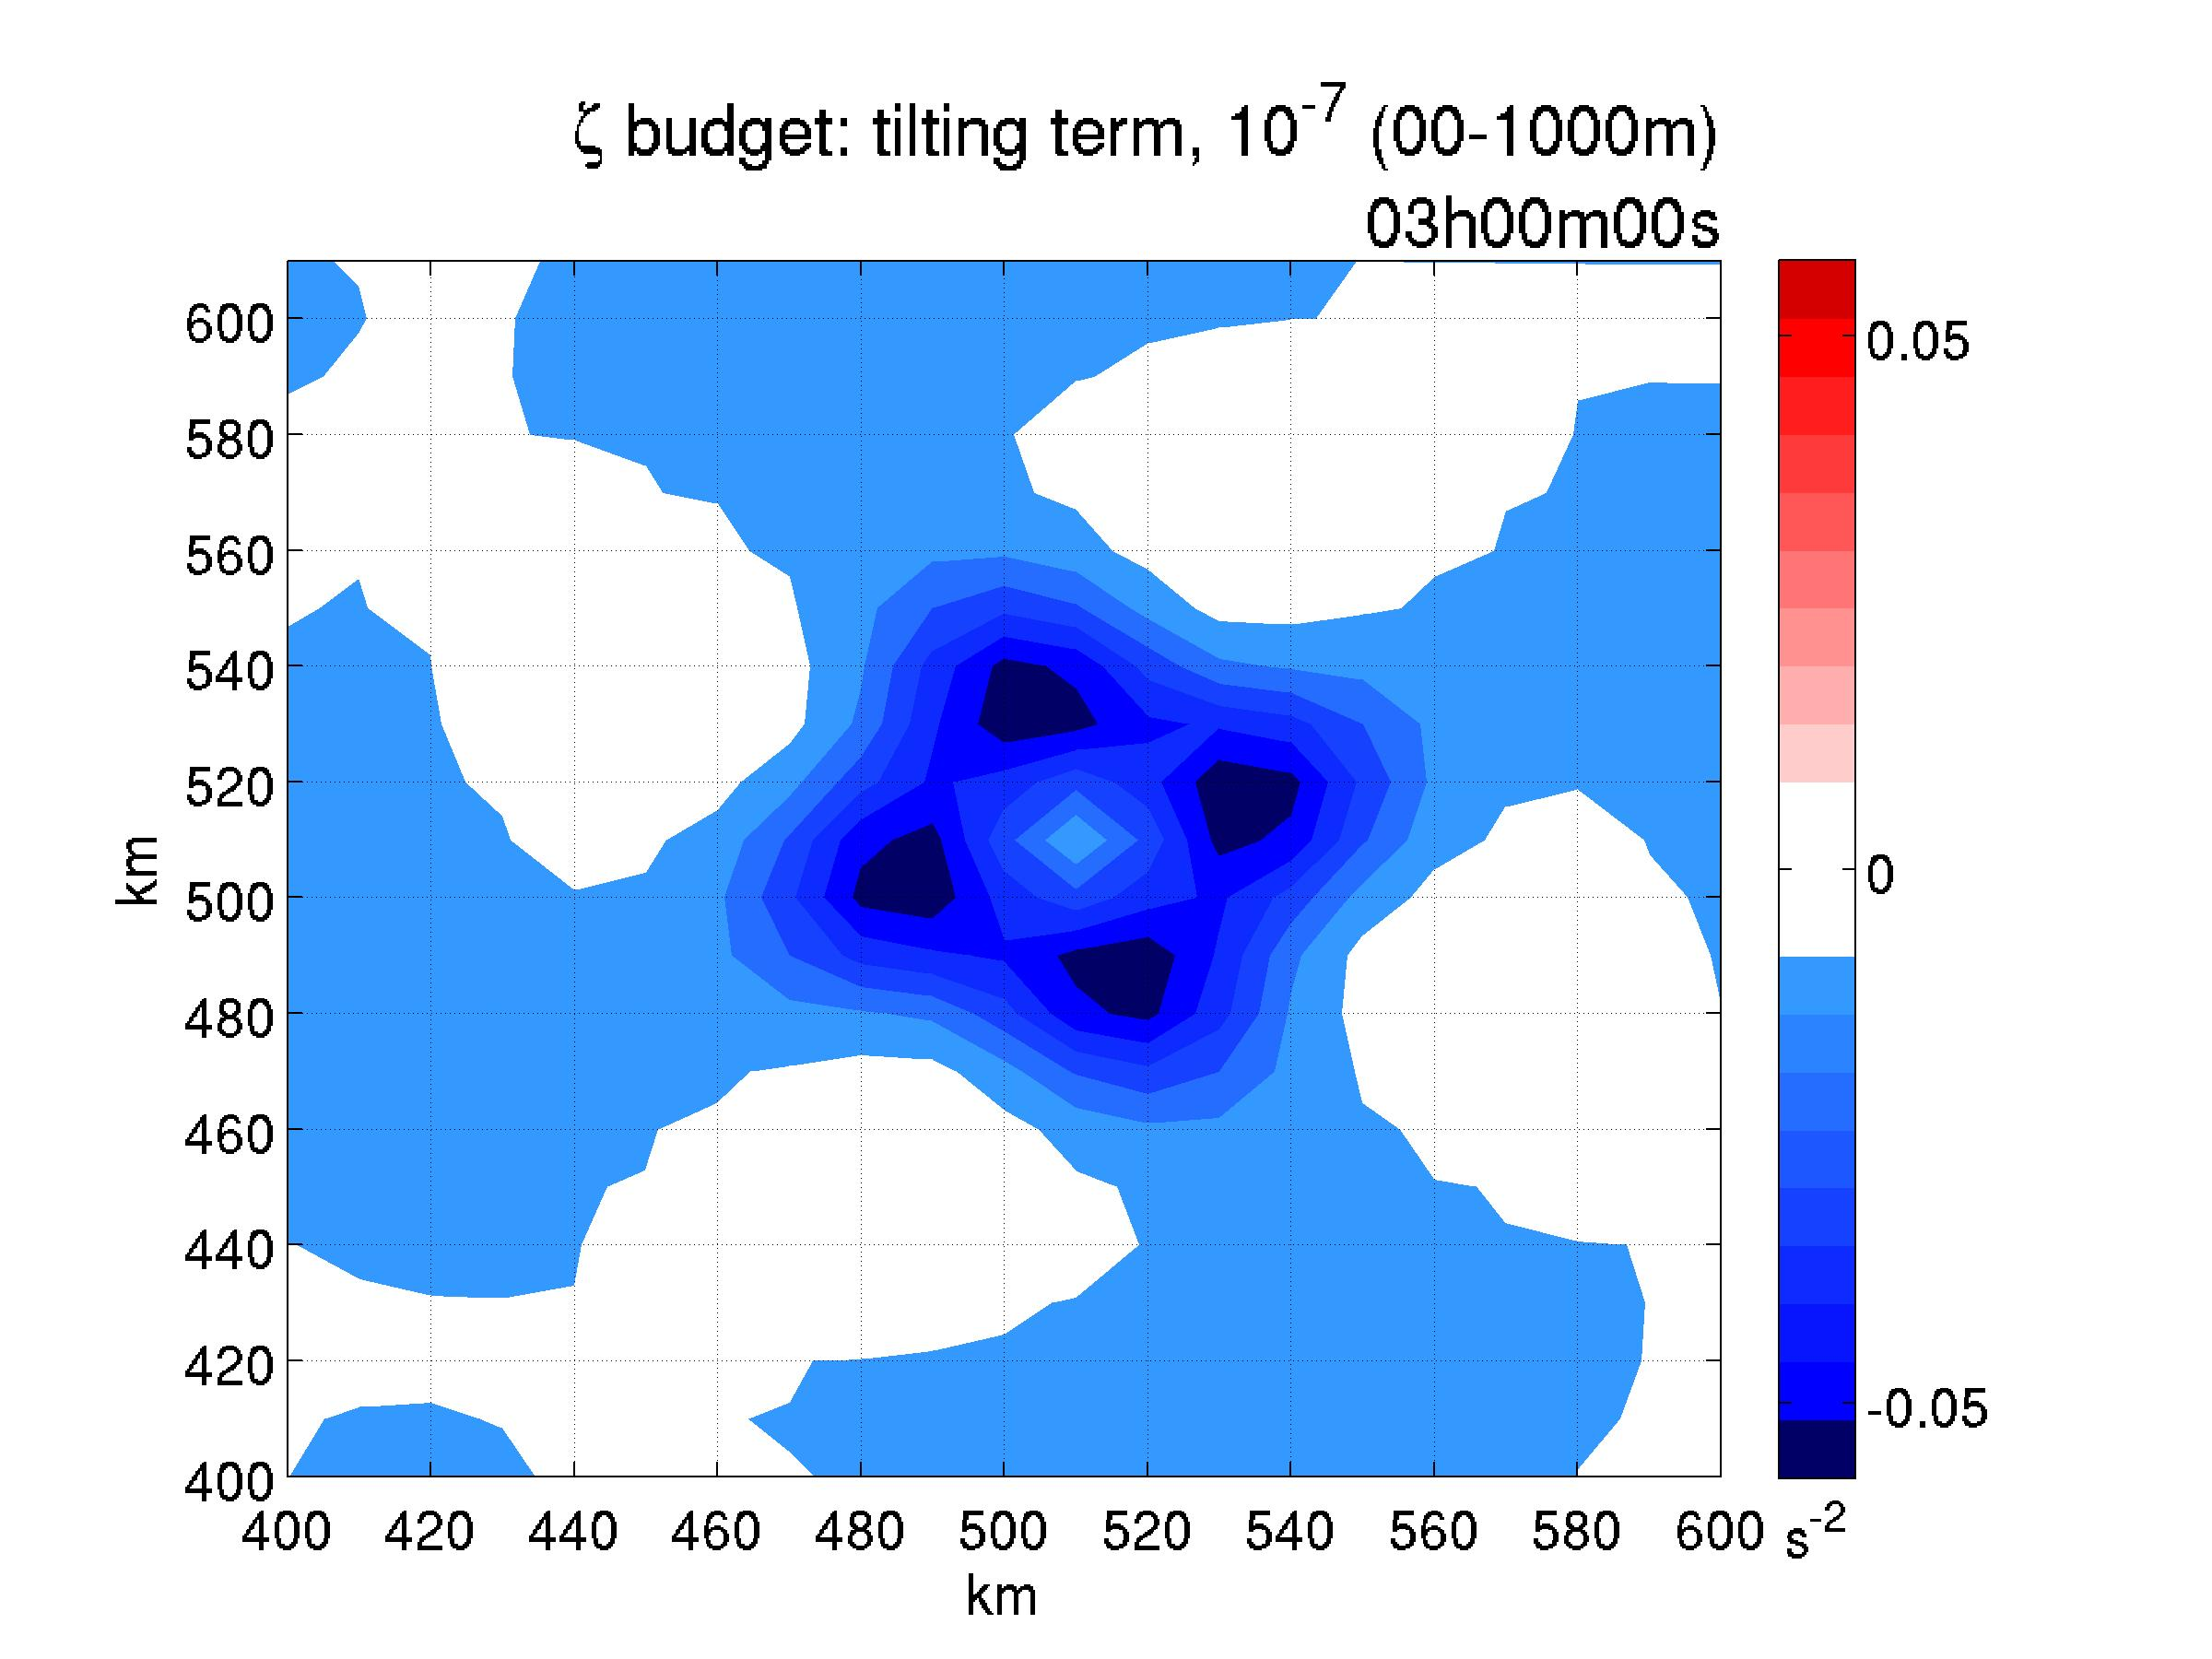
\includegraphics[width=\linewidth]{{./chapters/figures_results/ctrl_fields/vort_budget_tilt_z.x41-x62.y41-y61.ilev02.030000}.jpg}
		\caption{Слагаемое наклона, $\s^{-2}$.}
		\label{fig:ctrl_tilt03}
	\end{subfigure}
	\hfill
	\begin{subfigure}[t]{0.3\textwidth}
		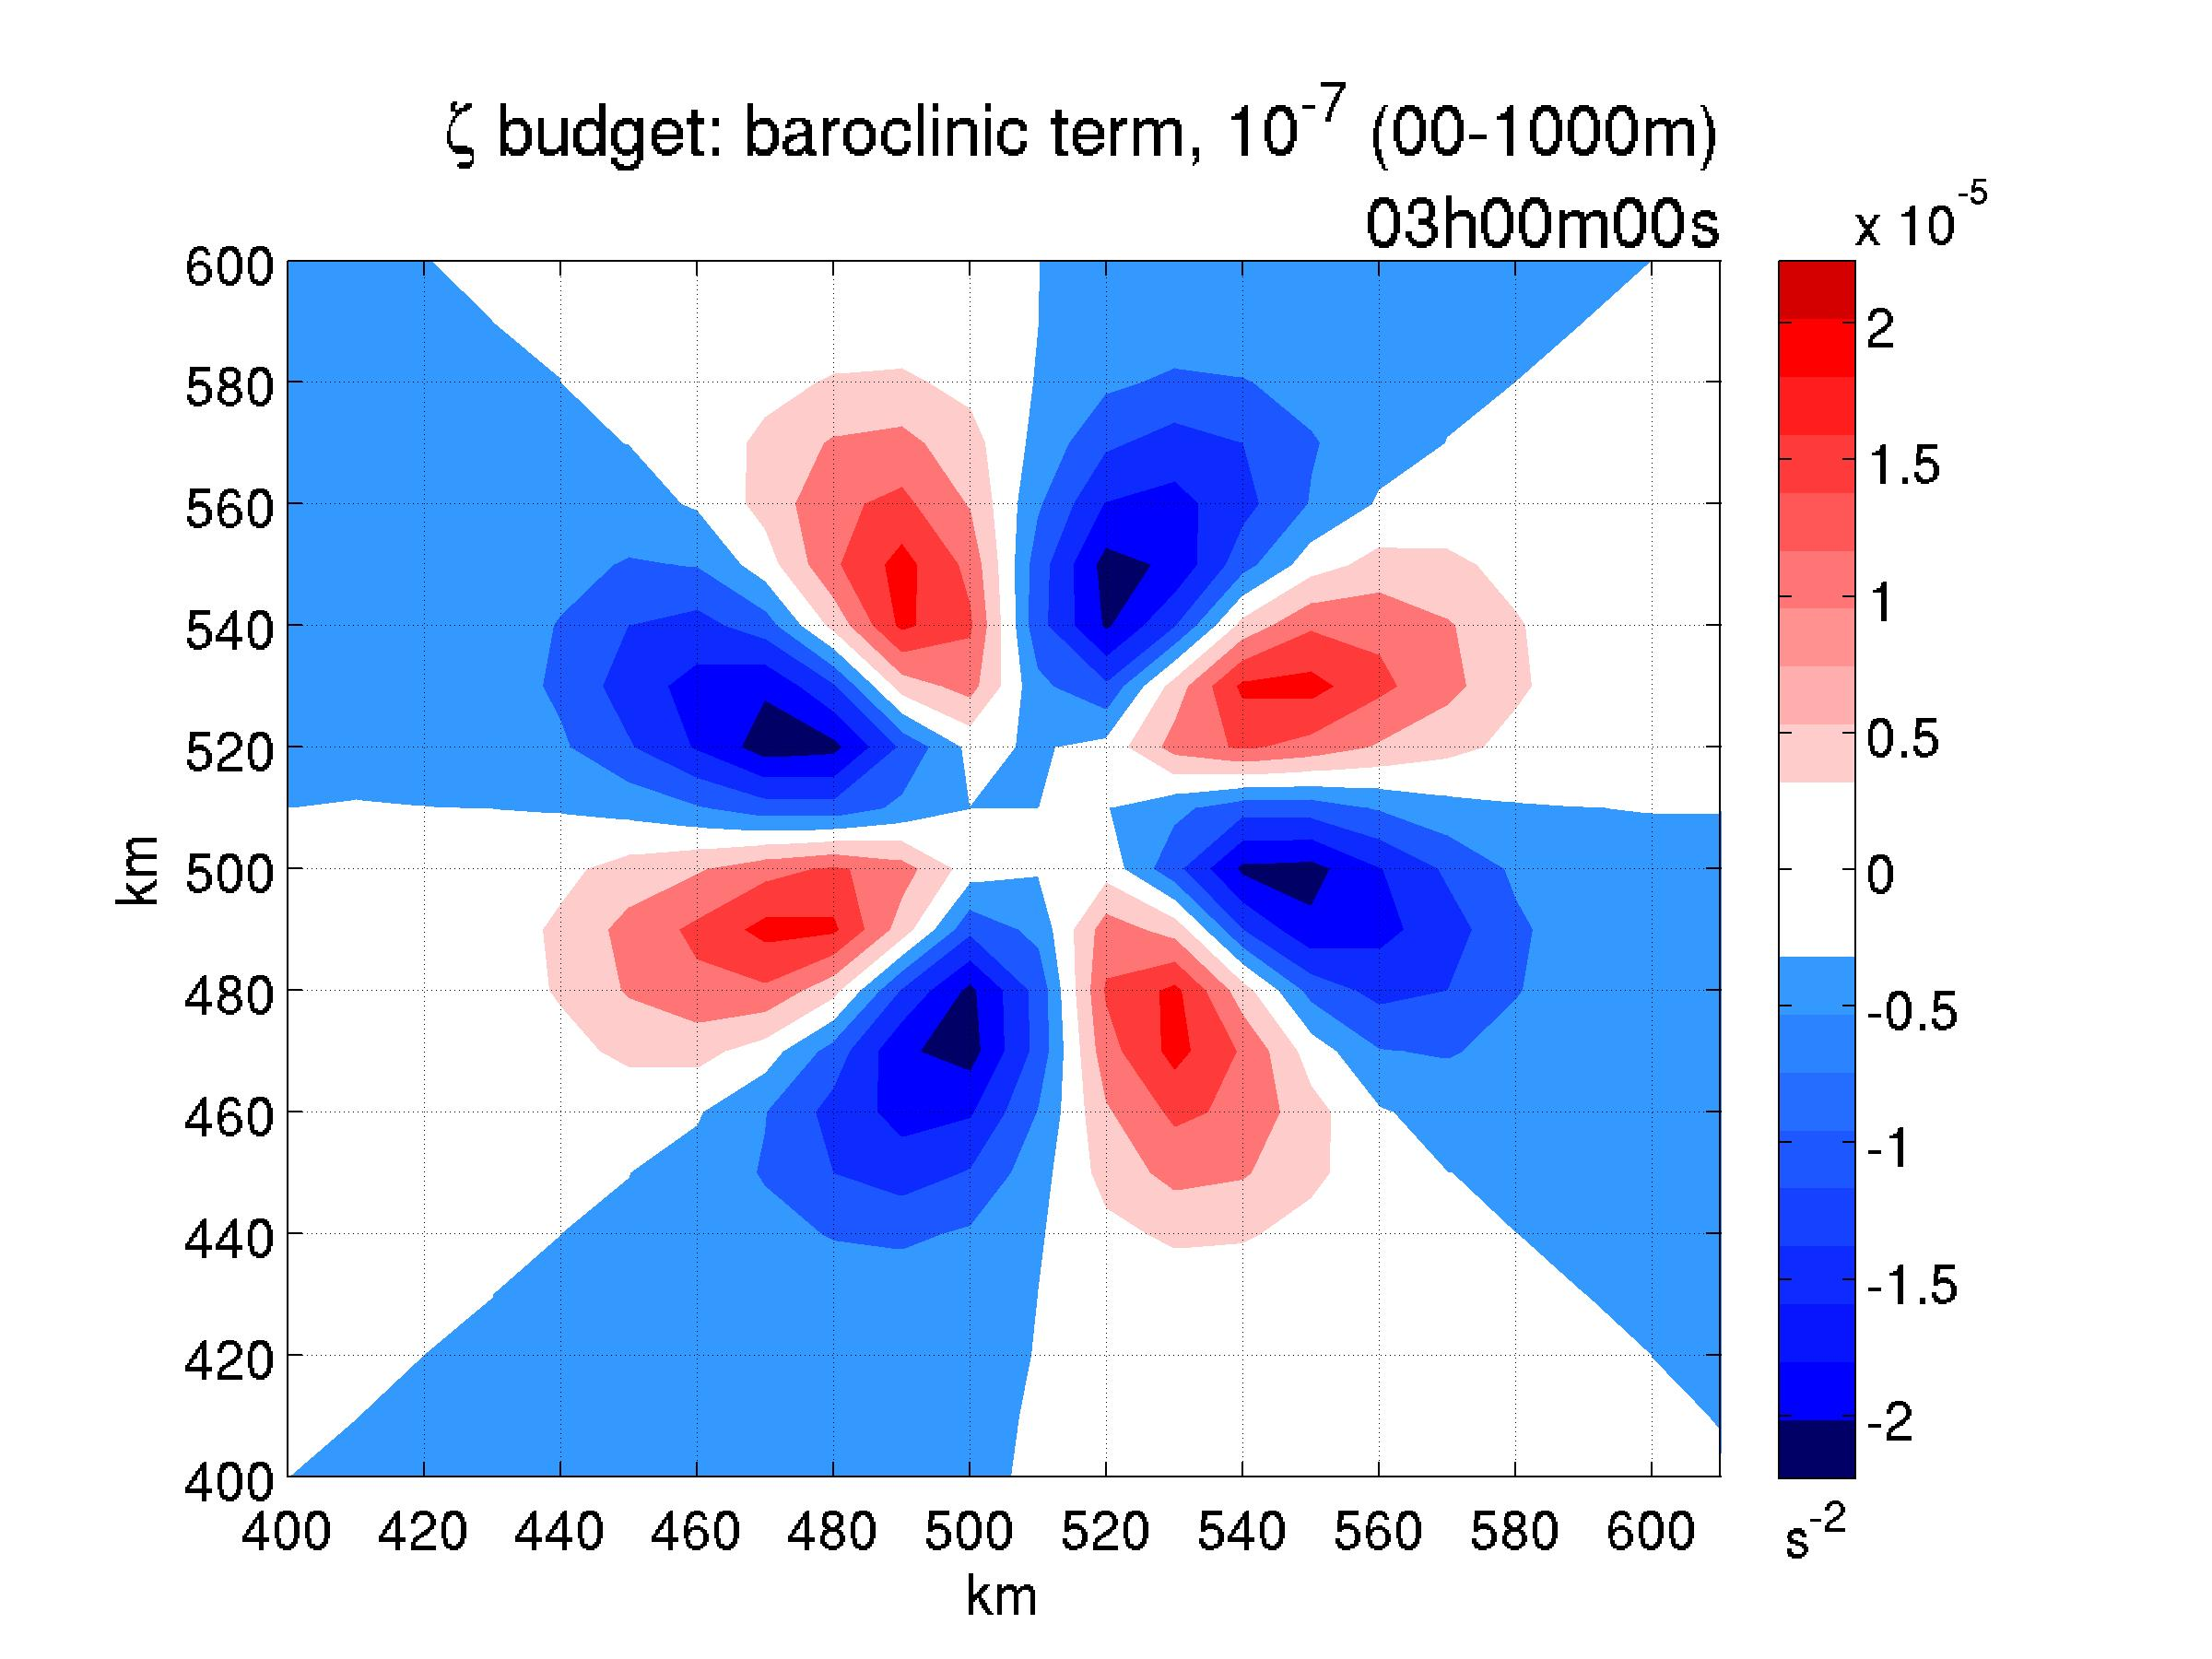
\includegraphics[width=\linewidth]{{./chapters/figures_results/ctrl_fields/vort_budget_bc_z.x41-x62.y41-y61.ilev02.030000}.jpg}
		\caption{Бароклинное слагаемое, $\s^{-2}$.}
		\label{fig:ctrl_bc03}
	\end{subfigure}
    \caption{Завихренность и бюджет завихренности в слое ниже $1000\m$. Область $200\times 200\km$, 3 час модельного времени.}
    \label{fig:ctrl_vortbud03}
\end{figure}

Равновесная часть движения формируется сразу после инициализации температурной аномалии. Подтверждением того, что наибольший вклад в развитие циркуляции имеет конвергенция массы, служит анализ уравнения завихренности \citep{Bluestein1992I} для $f$-плоскости (слагаемые, содержащие параметр $\beta=\partial f/ \partial y$ и силу трения опущены):
\begin{equation}
\label{eq:vorttend}
\pderiv{\zeta}{t}=-\vec{v}\cdot \nabla_z \zeta - w\pderiv{\zeta}{z} - (\zeta + f)\left(\pderiv{u}{x}+\pderiv{v}{y}\right) 
+ \vec{k}\cdot\left(\pderiv{\vec{v}}{z}\times\nabla w\right) + \vec{k}\cdot\left(\nabla p \times \nabla\alpha \right),
\end{equation}
где $\zeta$ --- вертикальная компонента вектора вихря скорости (завихренность), $\vec{v}=(u,v,w)$ --- вектор скорости, $\alpha=1/\rho$ --- удельный объем. Рассмотрим состояние эксперимента в 3 час модельного времени --- в момент, когда аномалия только что была инициализирована. На рис. \ref{fig:ctrl_vortbud03} представлены пространственное распределение компонент, входящих в правую часть ур. \ref{eq:vorttend}. Данные осреднены по вертикали в слое от $0$ до $1000\m$, в котором в течение всего времени наблюдаются наибольшие значения градиентов скорости.

Нетрудно заметить, что содержащее горизонтальную дивергенцию слагаемое (слагаемое растяжения) имеет наибольшие значения (рис. \ref{fig:ctrl_stretch03}), причем его экстремум совпадает с экстремумом тенденции завихренности (рис. \ref{fig:ctrl_vorttend03}) и они близки по значению. Недостающую часть тенденции вихря составляет вертикальная адвекция. Величина завихренности уже достаточно велика в данный момент (приблизительно в 2 раза меньше, чем значение параметра Кориолиса), а скорость ее роста говорит о том, что меньше, чем через час значения удвоятся. Бароклинное слагаемое (ур. \ref{eq:vorttend}, последнее слагаемое) --- произведение градиентов давления и плотности --- имеет значения на 3--4 порядка меньшие остальных членов (рис. \ref{fig:ctrl_bc03}), и это соотношение сохраняется в течение всего эксперимента. Поэтому далее бароклинное слагаемое рассматриваться не будет.

\subsection{Эволюция вихря}
Общую картину динамики вихря дают графики изменения максимума завихренности в нижней тропосфере и минимума аномалии приземного давления (\ref{}). Более детально структура вихря будет рассмотрена в следующем разделе. В контрольном эксперименте не удалось получить устойчивый вихрь: интенсивность начального возмущение с возрастающей скоростью увеличивается, пока не компоненты вектора скорости не достигают критических для численной схемы модели значений. Другими словами, в контрольном эксперименте, как и в большинстве других (см. далее), вихрь растет, не достигая устойчивой фазы и не диссипируя после этого.

\begin{wrapfigure}{L}{0.5\textwidth}
\begin{center}
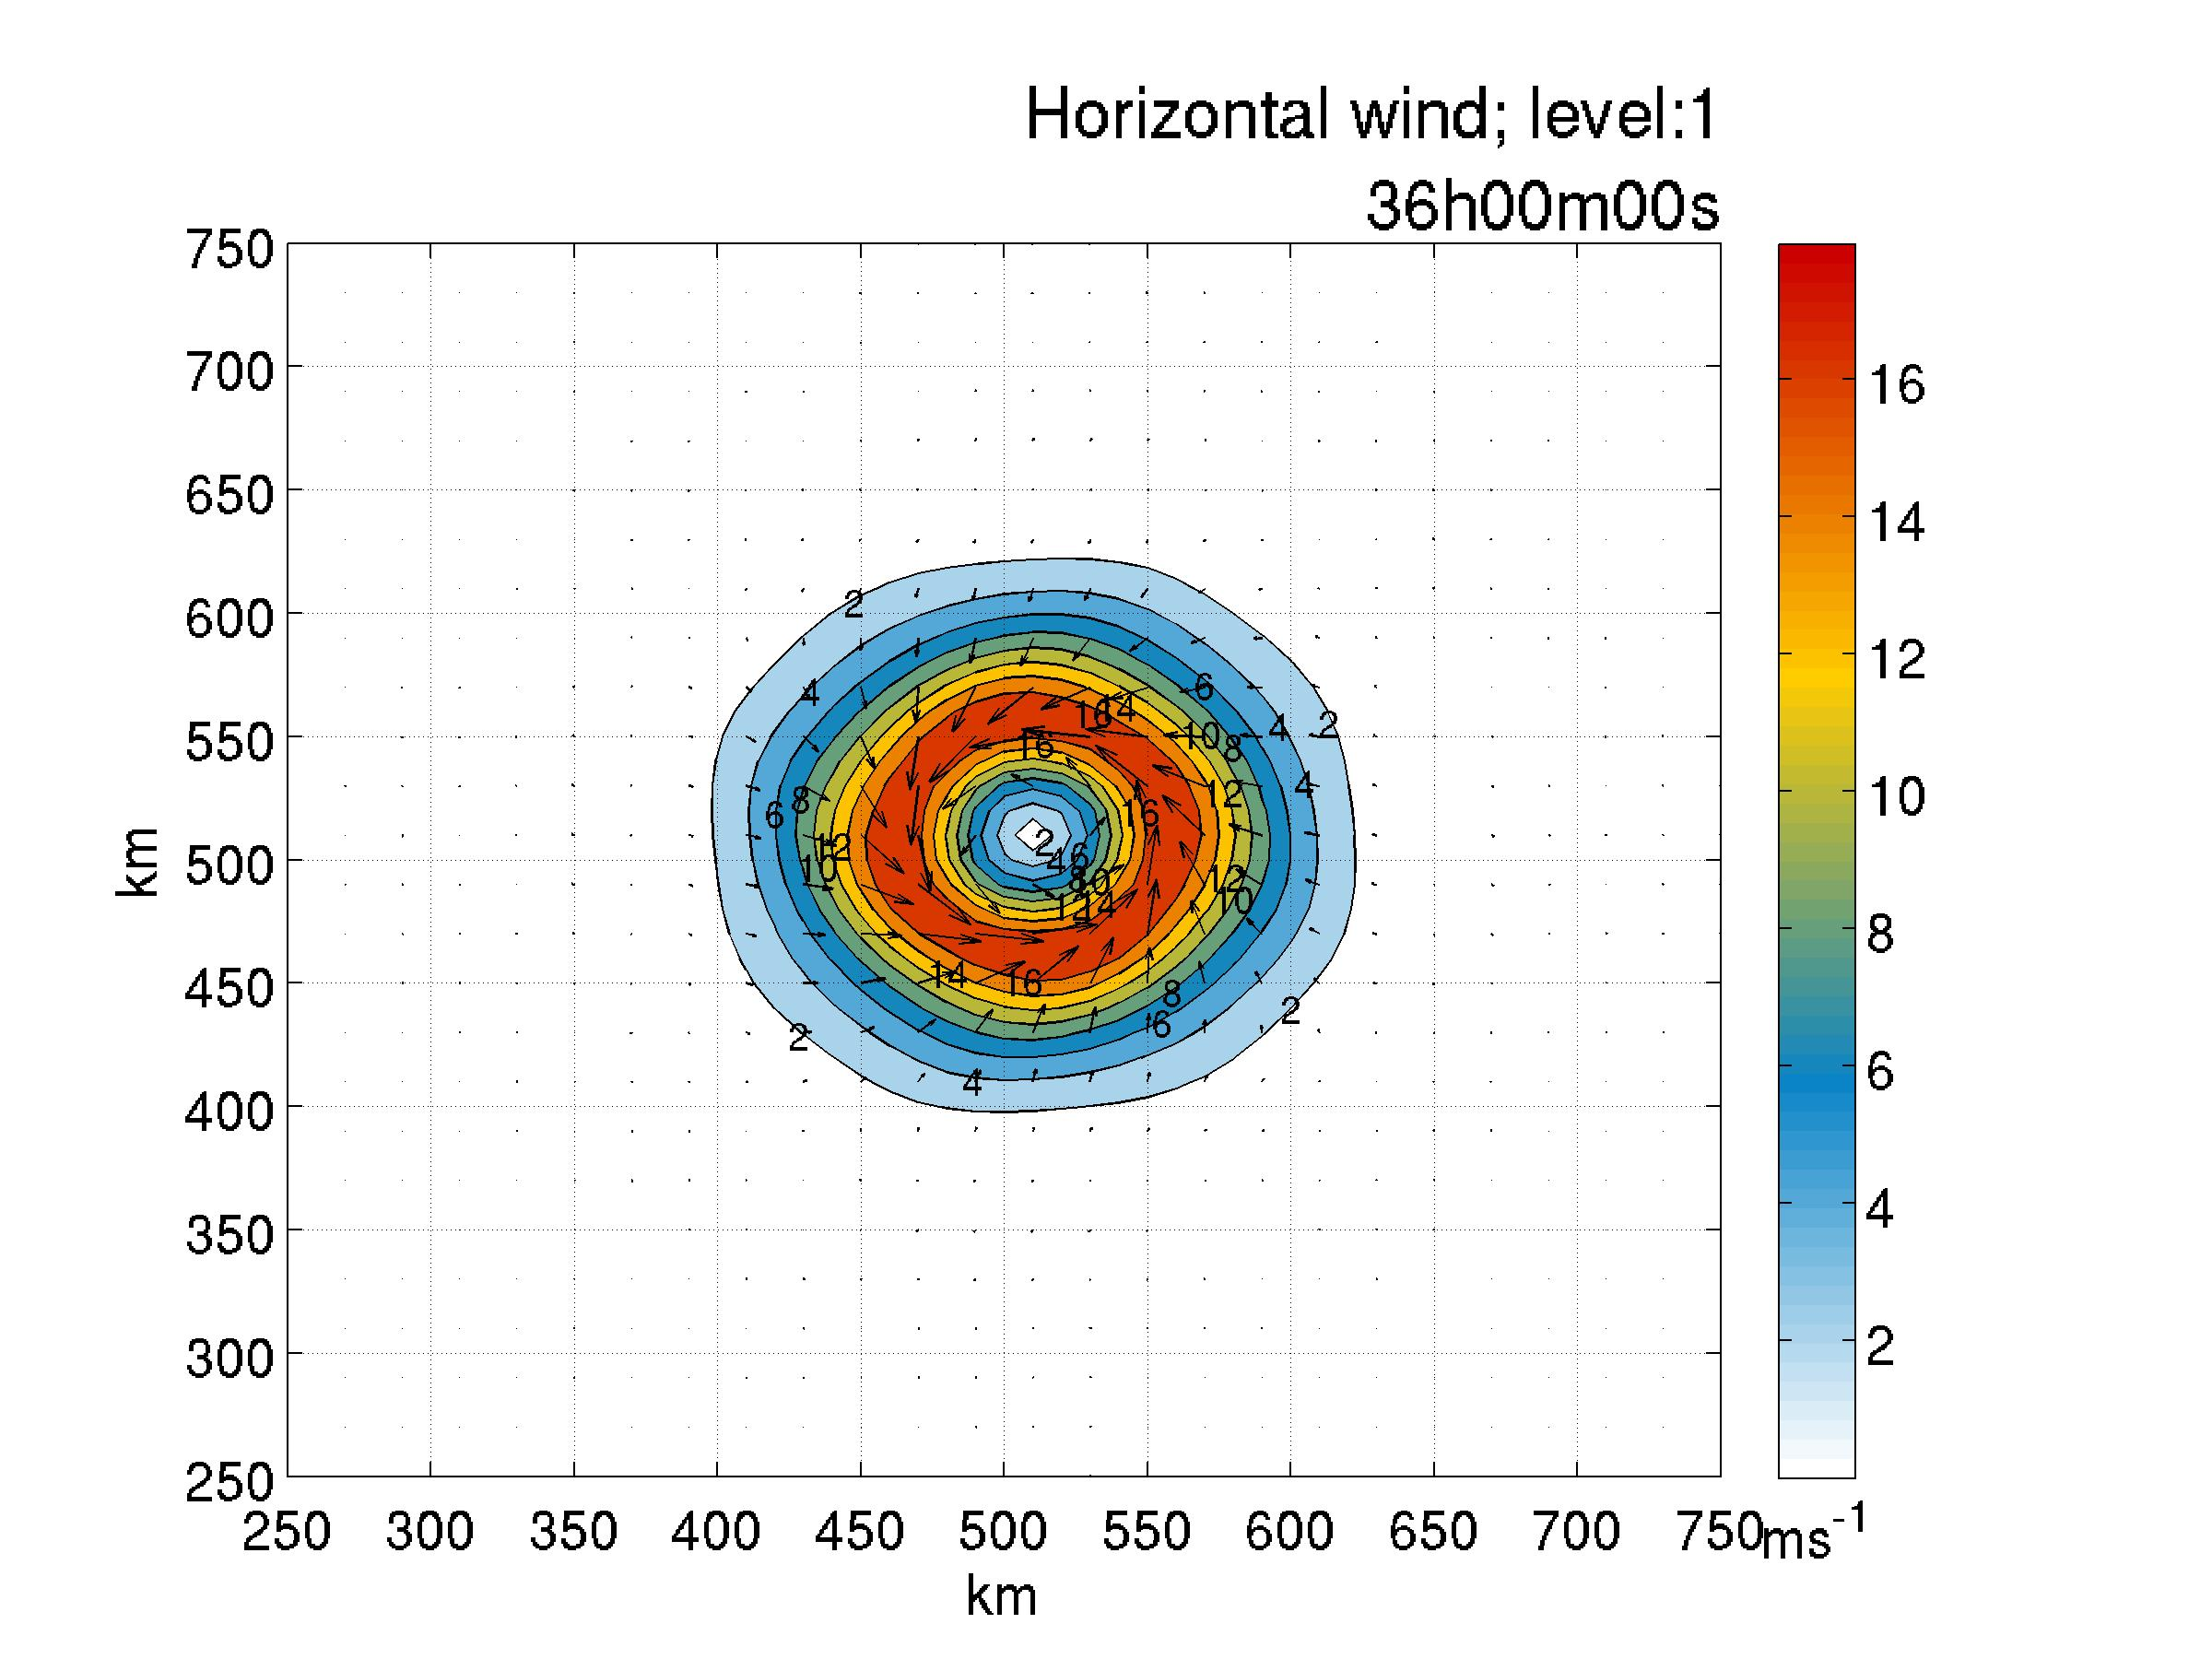
\includegraphics[width=\linewidth]{{./chapters/figures_results/ctrl_fields/VectorWind_z.x26-x76.y26-y76.ilev01.360000}.jpg}
\end{center}
\caption{Поле горизонтальной скорости ветра  (фокус $500\times 500\km$). Эксперимент CTRL. 36 час модельного времени.}
\label{fig:ctrl_hwind}
\end{wrapfigure} 

Уже в начале эксперимента относительная завихренность начинает превышать планетарную завихренность, которая для данной области равняется $\approx 1.37\pers$. Поэтому можно говорить о том, что динамика мезоциклона полностью описывается относительной завихренностью и почти не зависит от планетарной компоненты в течение своего жизненного цикла. Максимальное значение завихренности достигается на 43 ч. модельного времени и составляет $7.6\times 10^{-3}\pers$. В конце эксперимента достигается и наибольшее по модулю падение приземного давления ($-43.6\hpa$). Здесь и далее под этим понимается разность между минимальным приземным давлением и средним по области приземным давлением:
\begin{equation} \label{eq:slpanom}
SLP_{anom}=SLP_{min}-\overline{SLP}.
\end{equation}

\begin{wrapfigure}{L}{0.5\textwidth}
\begin{center}
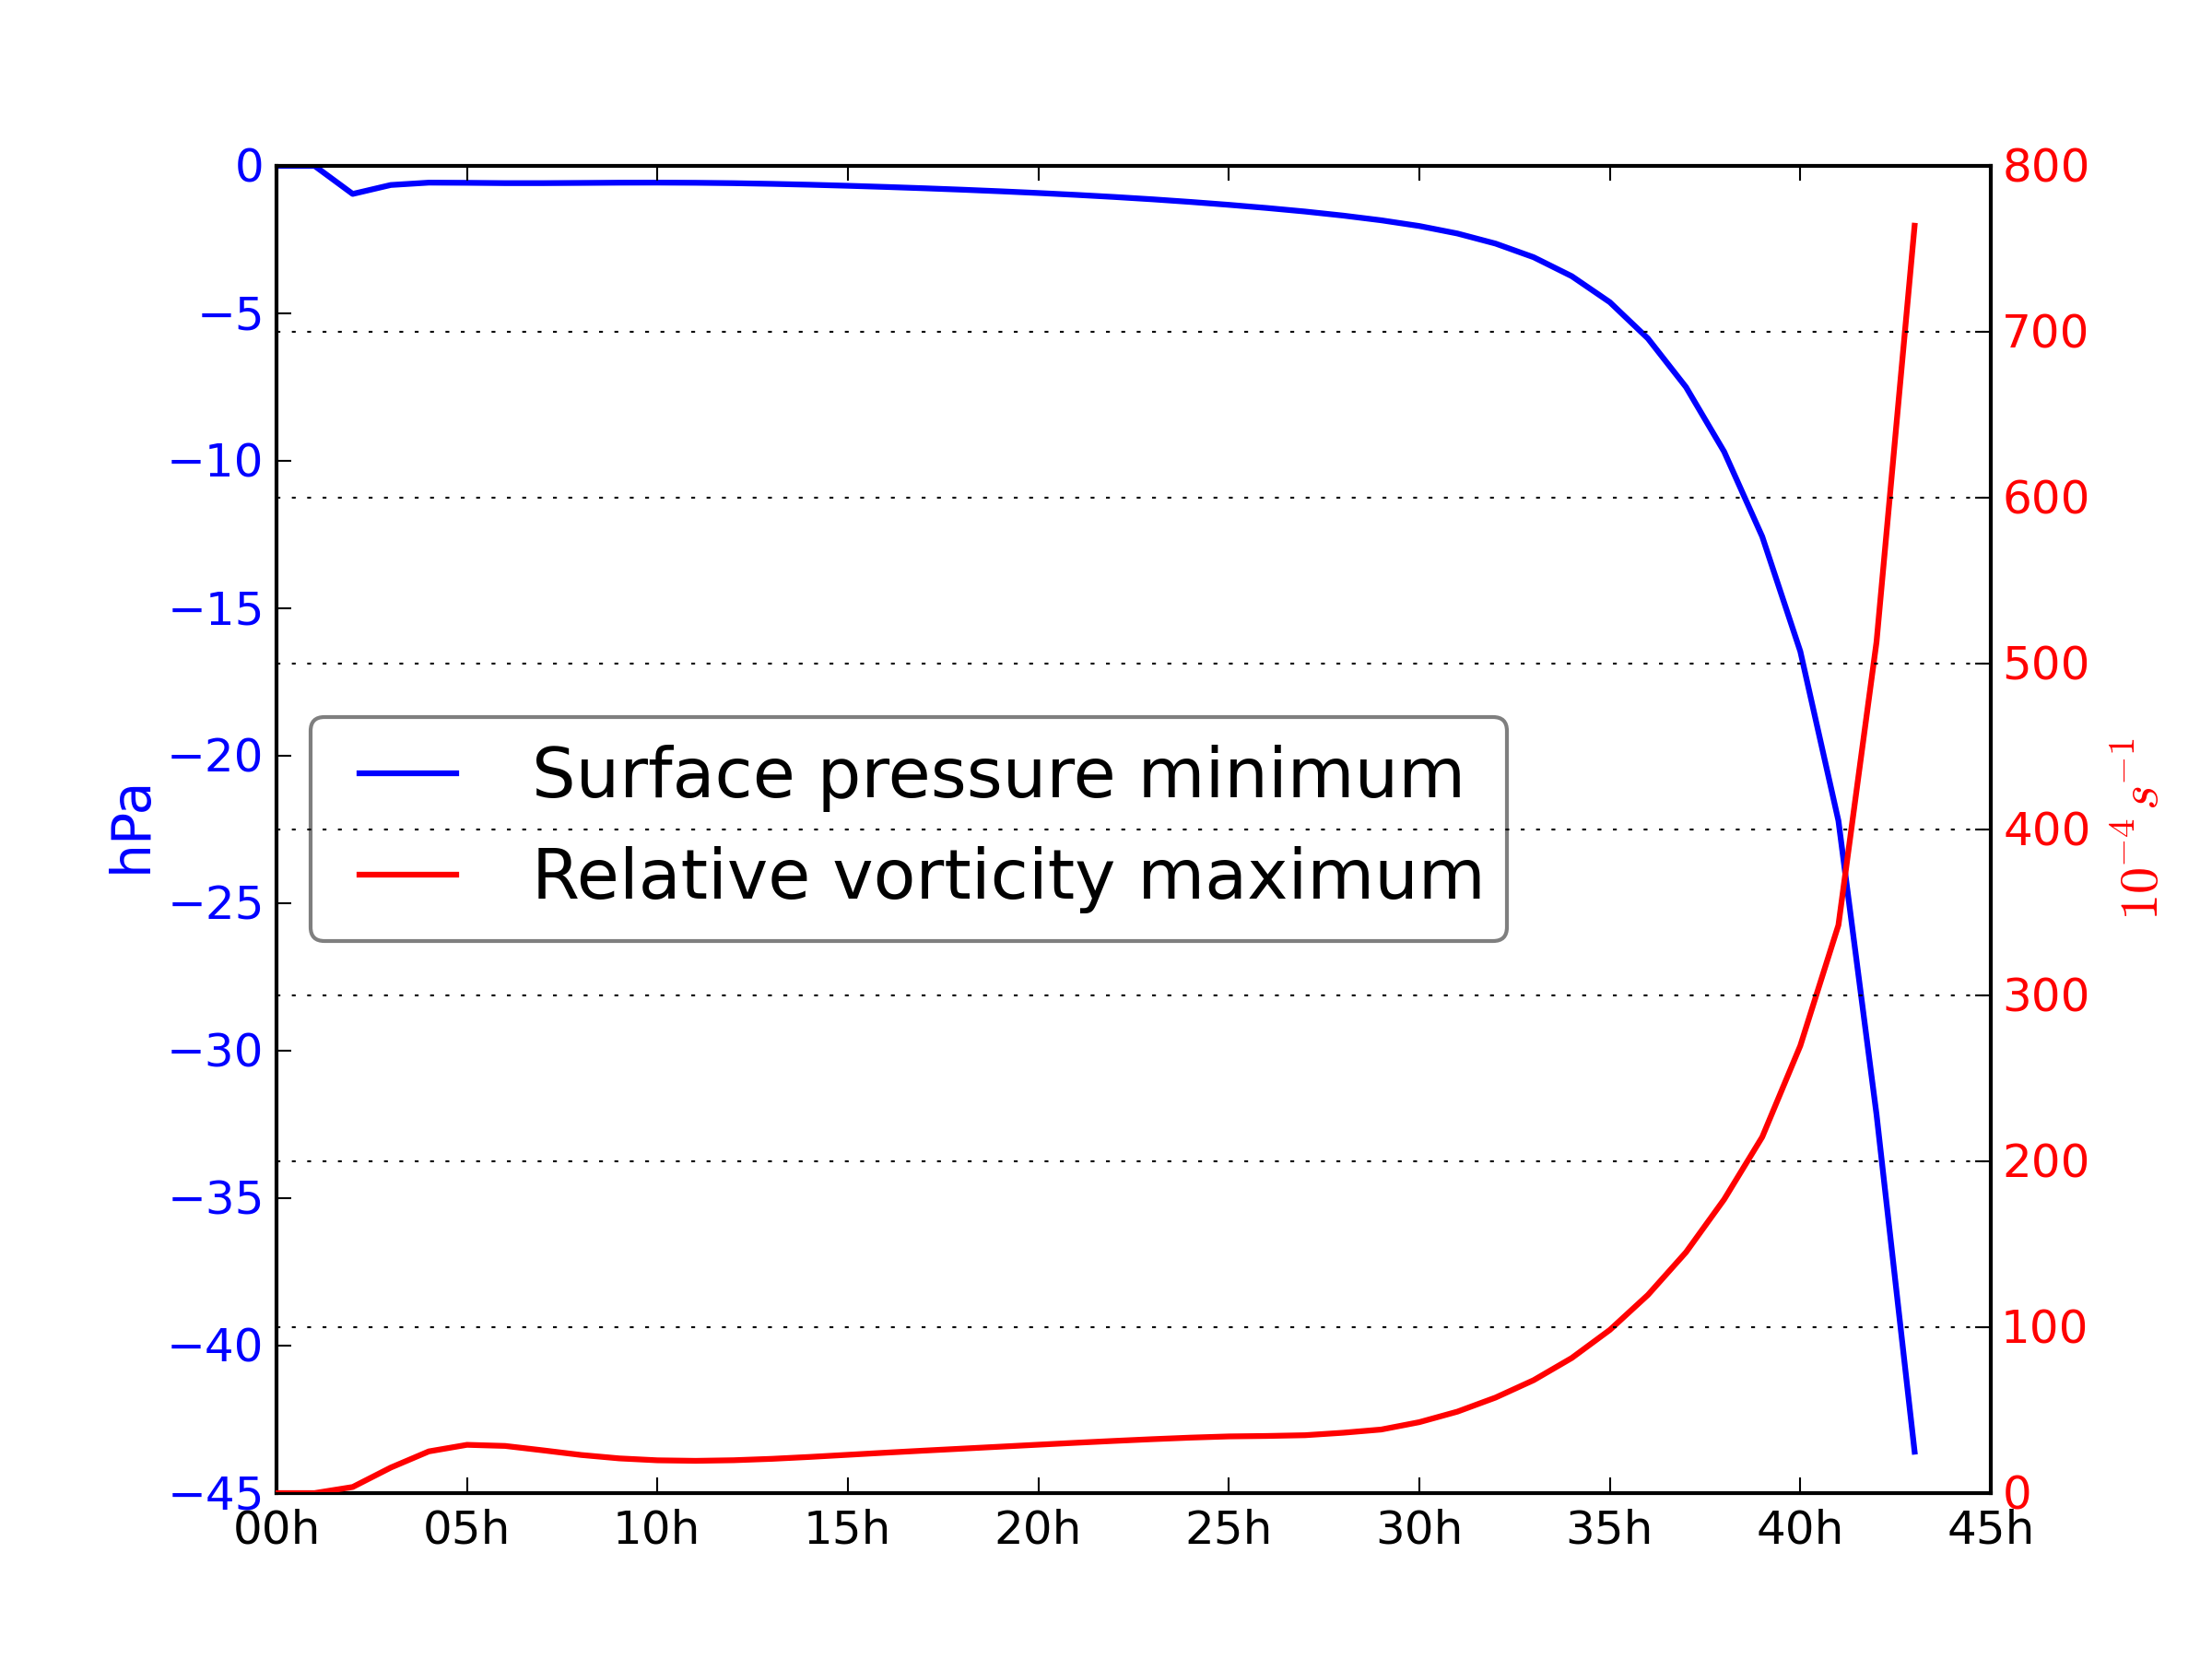
\includegraphics[width=\linewidth]{{./chapters/figures_results/slpmin_vortmax.00h-43h.ctrl}.png}
\end{center}
\caption{Изменение аномалии приземного давления и максимальной завихренности во времени. Эксперимент CTRL.}
\label{fig:ctrl_slpminvortmax}
\end{wrapfigure} 

Исходя из представленных графиков, можно заключить, что эволюция вихря происходила поступательно, без каких-либо смен режимов, за исключением испускания волн на начальной стадии. Из рис. \ref{fig:ctrl_slpminvortmax} также видно, что форма кривых изменения аномалии давления и максимума завихренности очень схожа, поэтому глубину циклона можно оценивать и первым, и вторым параметром \citep{YanaseEtAl2004}.

\subsection{Структура развитого вихря}
Для понимания механизма развития полярного мезоциклона логично остановиться на анализе его структуры в стадии достаточного развития, основываясь на горизонтальных и вертикальных разрезах полей метеовеличин за 36 час развития (12 часов вторых суток интегрирования), когда скорость приземного ветра превысила $15\mps$ (рис. \ref{fig:ctrl_hwind}).

Форма циклонического возмущения ожидаемо остается осесимметричной, в силу отсутствия фонового потока. Изначачально положительная температурная аномалия интенсифицируется: приблизительно в два раза увеличивается ее радиус (до $100\km$), а высота возрастает до $6\km$ (рис. \ref{fig:ctrl_ptdev_rz}). В соответствии с полем температуры находится и поле давления, аномалия которого у поверхности также достигает радиуса $100$--$120\km$. 

\begin{figure}[ht]
	\centering
	\begin{subfigure}[t]{0.45\textwidth}
		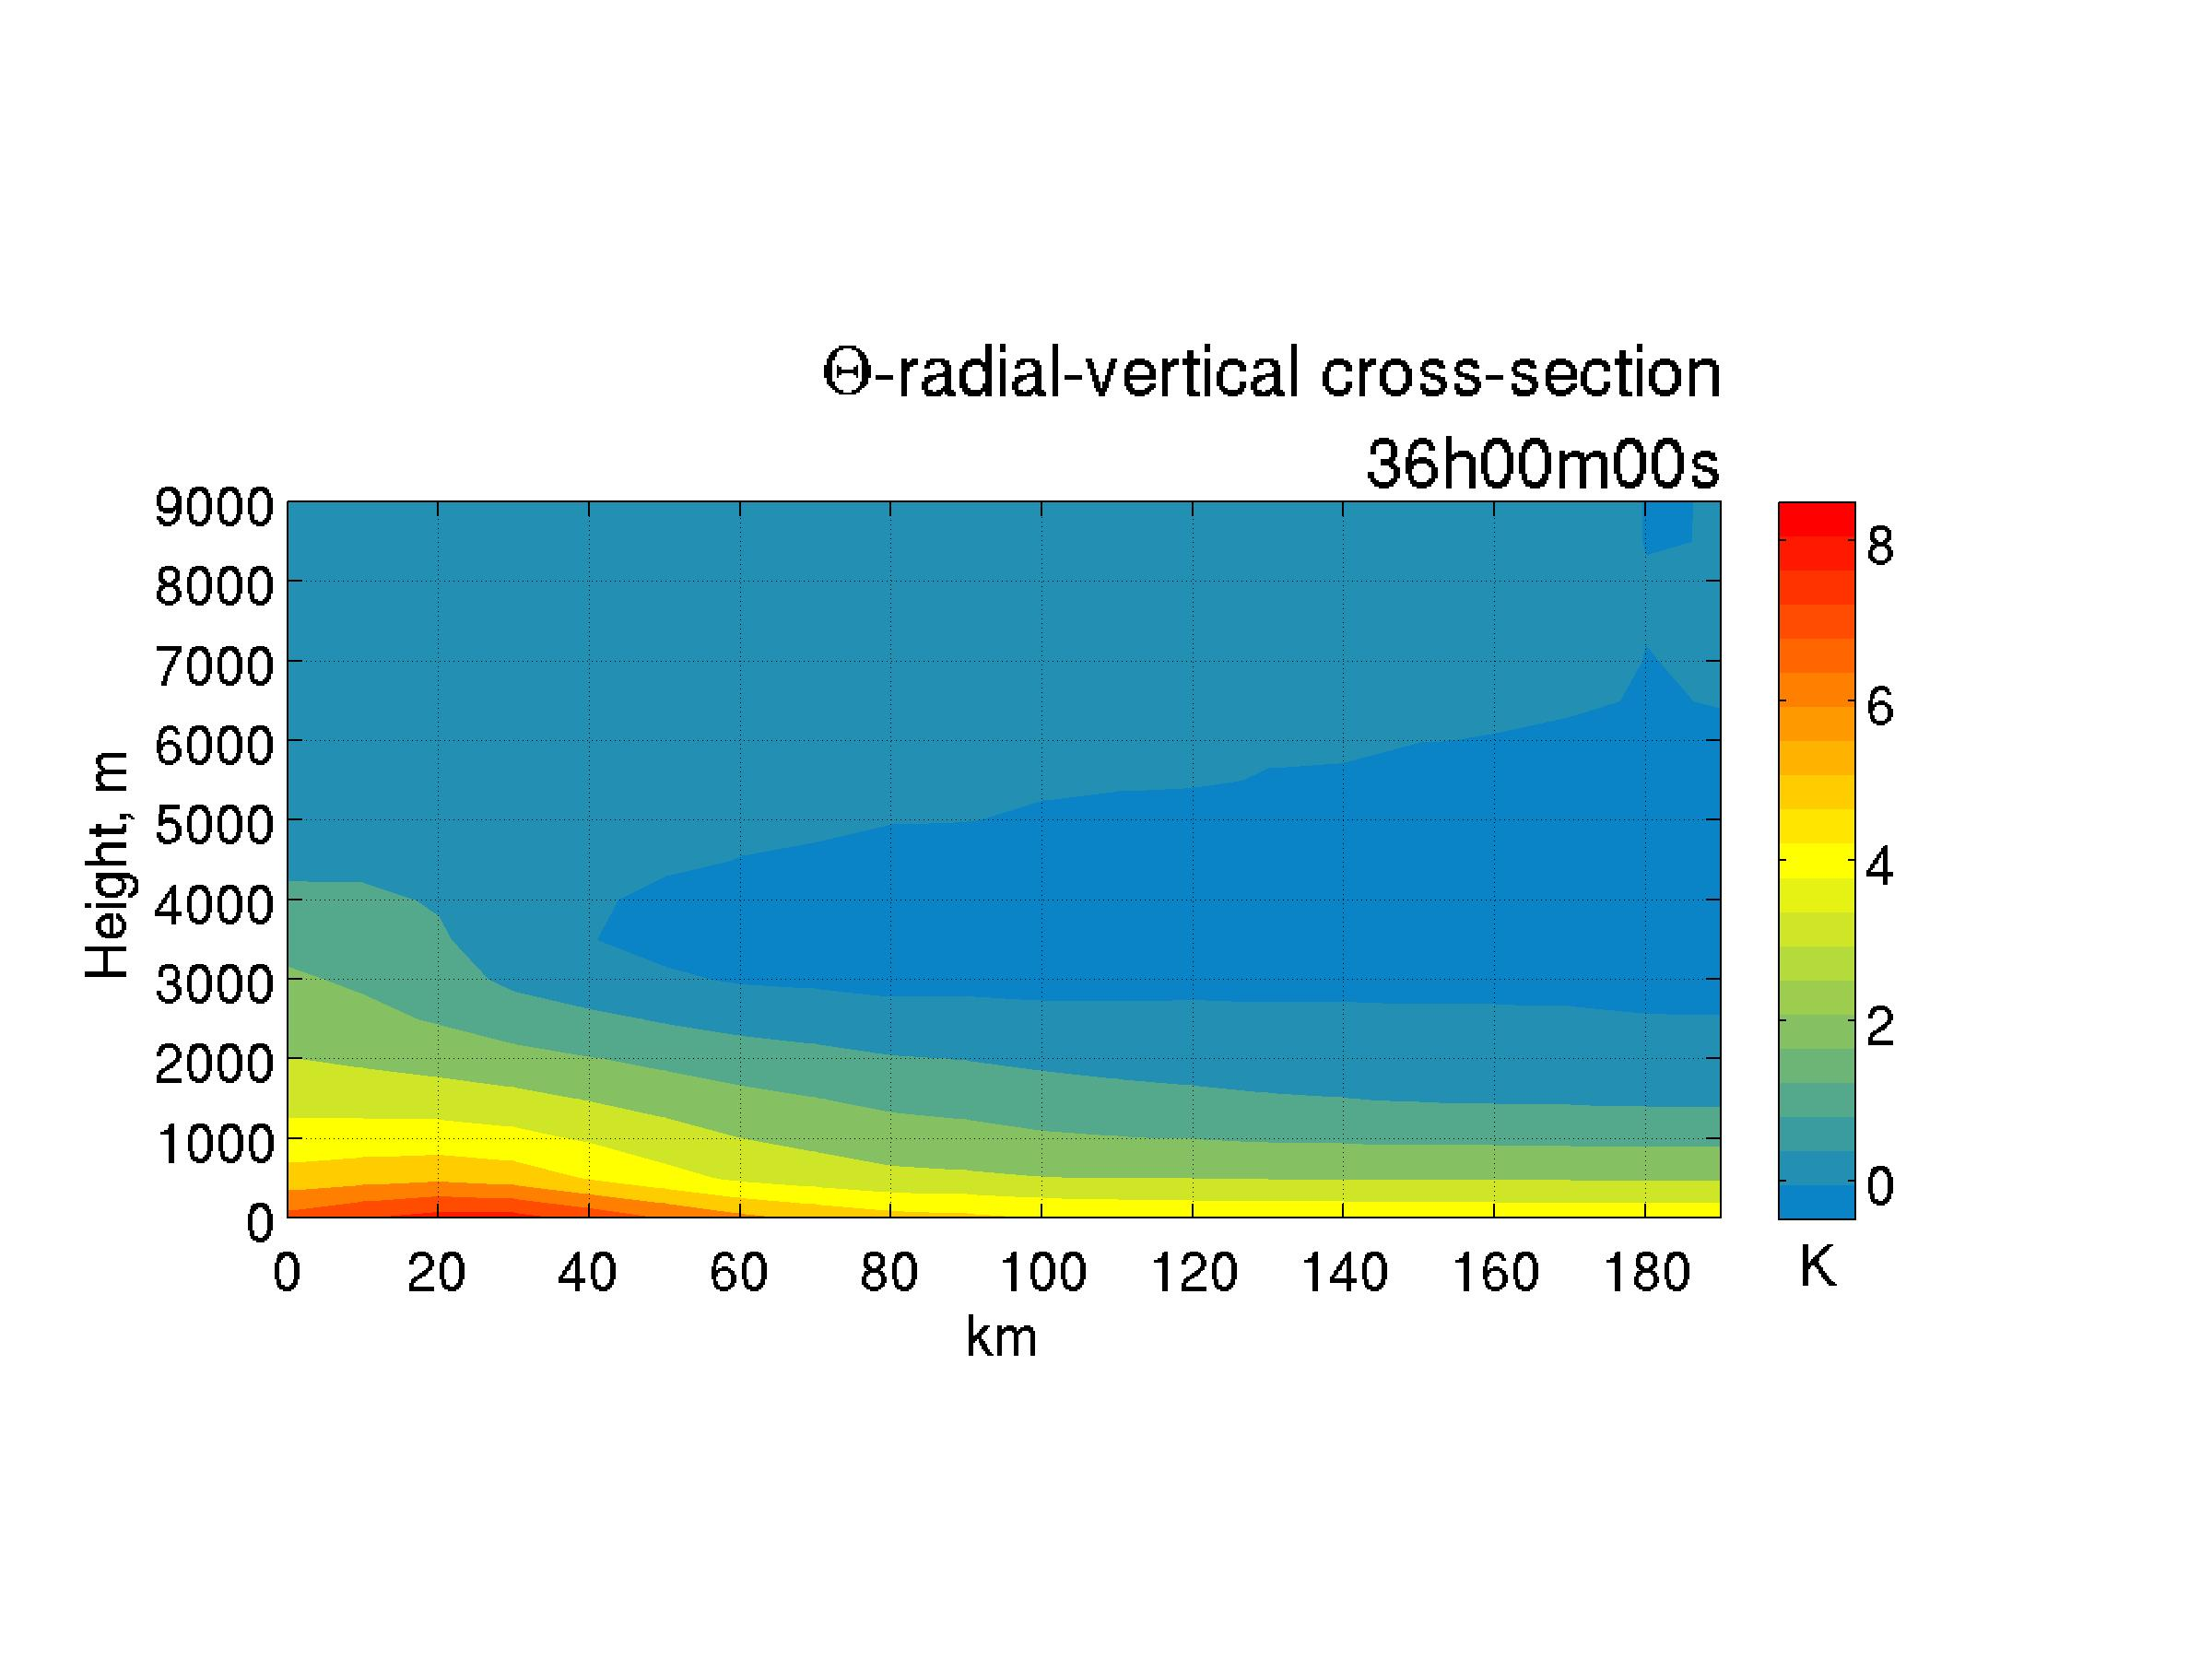
\includegraphics[width=\linewidth]{{./chapters/figures_results/ctrl_fields/ptdev_rz_z.ix52.360000}.jpg}
		\caption{Отклонения потенциальной температуры от фоновой ($\theta'$), $\K$.}
        \label{fig:ctrl_ptdev_rz}
	\end{subfigure}
	\hfill
	\begin{subfigure}[t]{0.45\textwidth}
		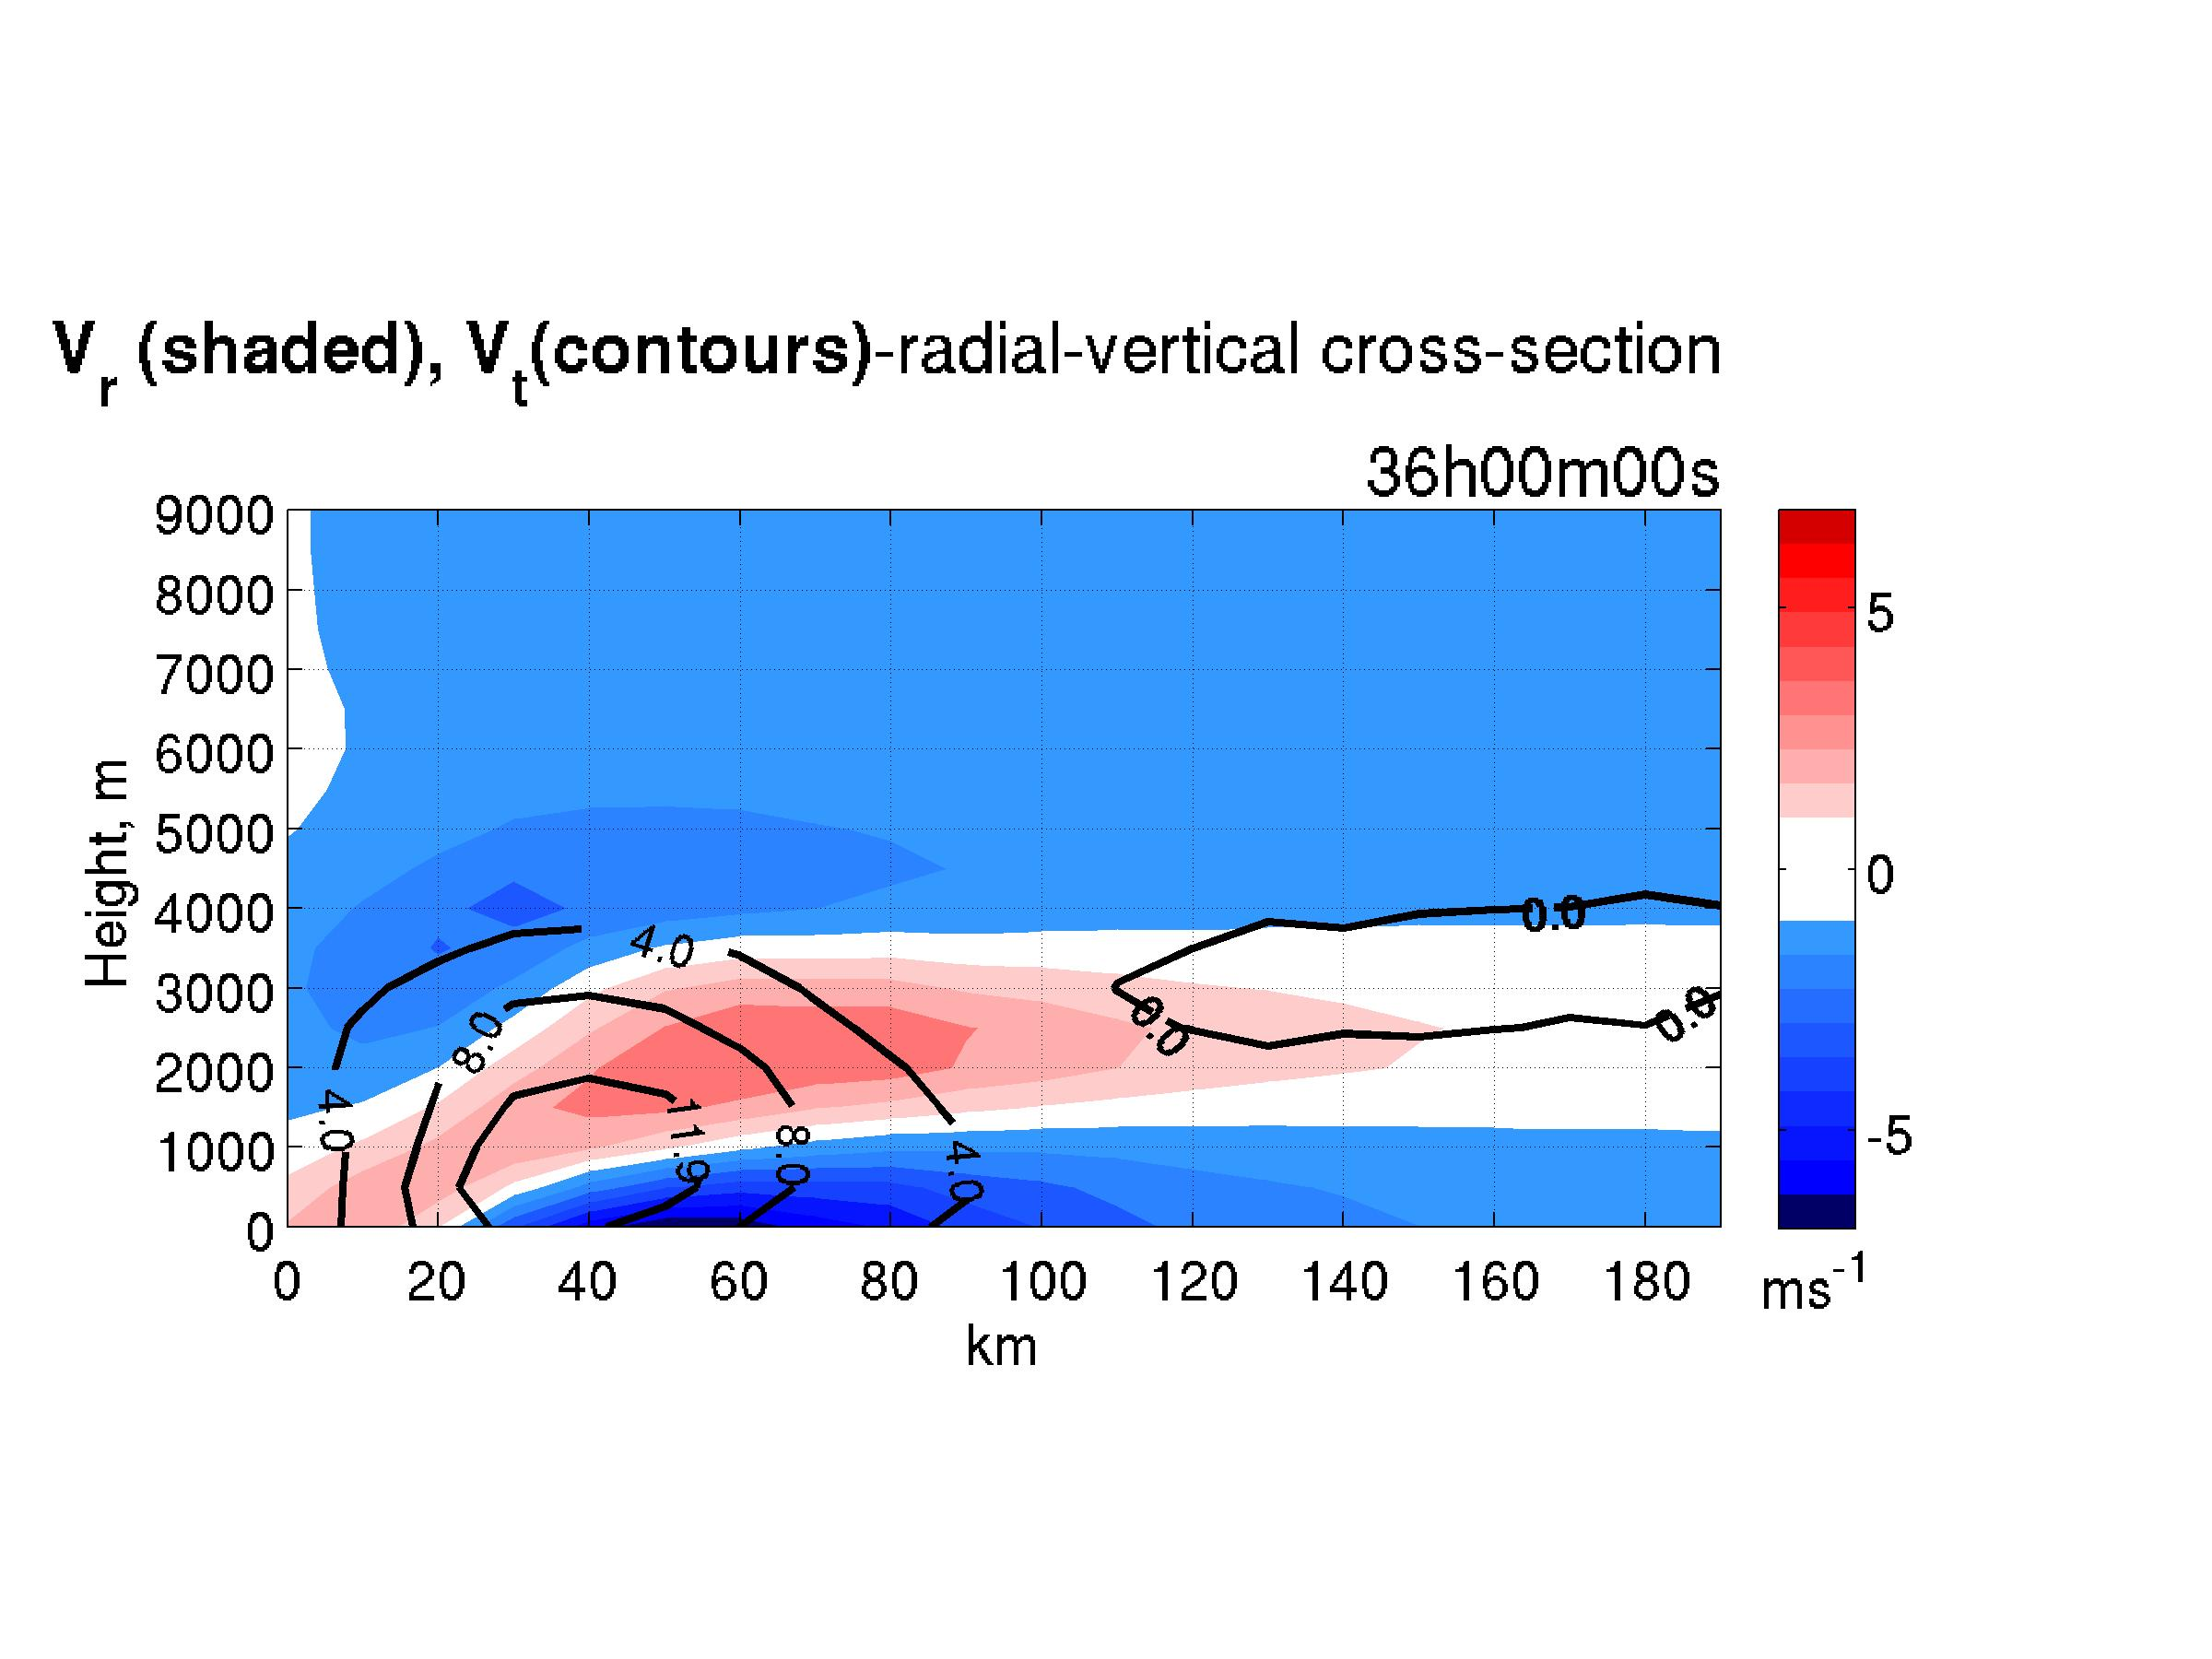
\includegraphics[width=\linewidth]{{./chapters/figures_results/ctrl_fields/vrvt_rz_z.ix52.360000}.jpg}
		\caption{Радиальная $v_r$ (цвет) и тангенциальная $v_t$ (контуры) компоненты скорости ветра, $\mps$.}
		\label{fig:ctrl_vrvt_rz}
	\end{subfigure}
	\hfill
    \begin{subfigure}[t]{0.45\textwidth}
		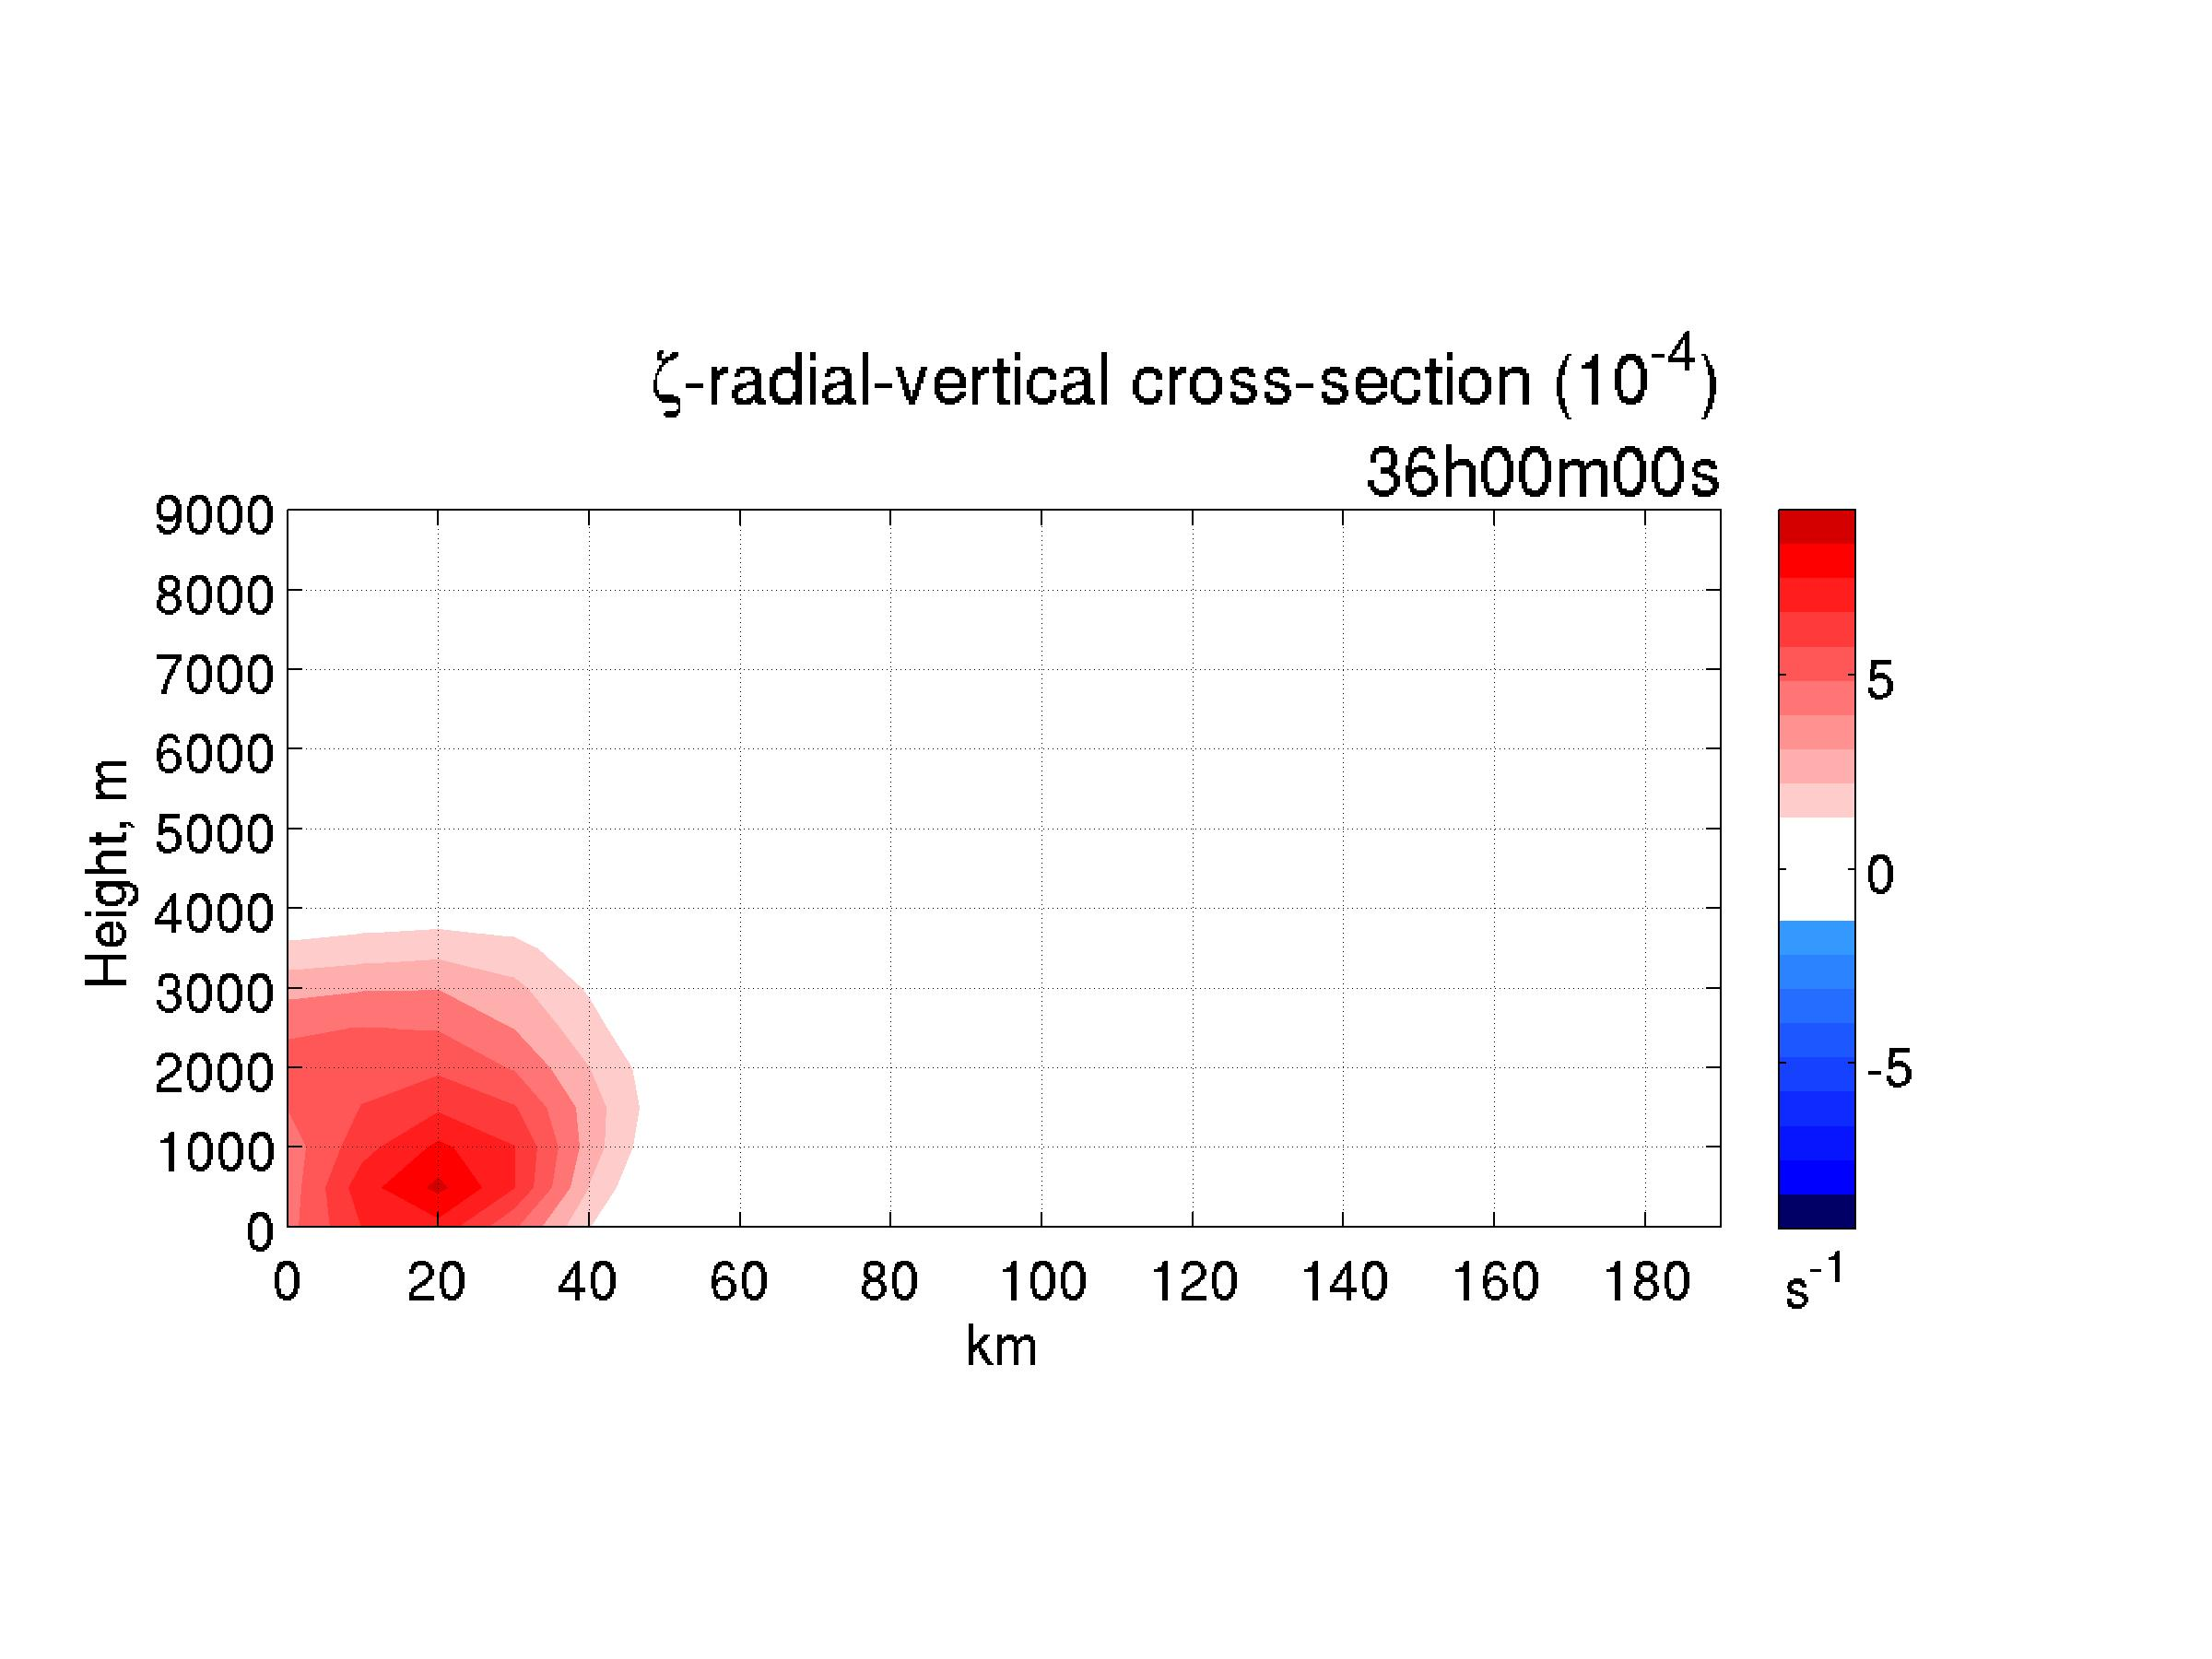
\includegraphics[width=\linewidth]{{./chapters/figures_results/ctrl_fields/vort_rz_z.ix52.360000}.jpg}
		\caption{Относительная завихренность ($\zeta$), $\pers$.}
		\label{fig:ctrl_vort_rz}
	\end{subfigure}
	\hfill
	\begin{subfigure}[t]{0.45\textwidth}
		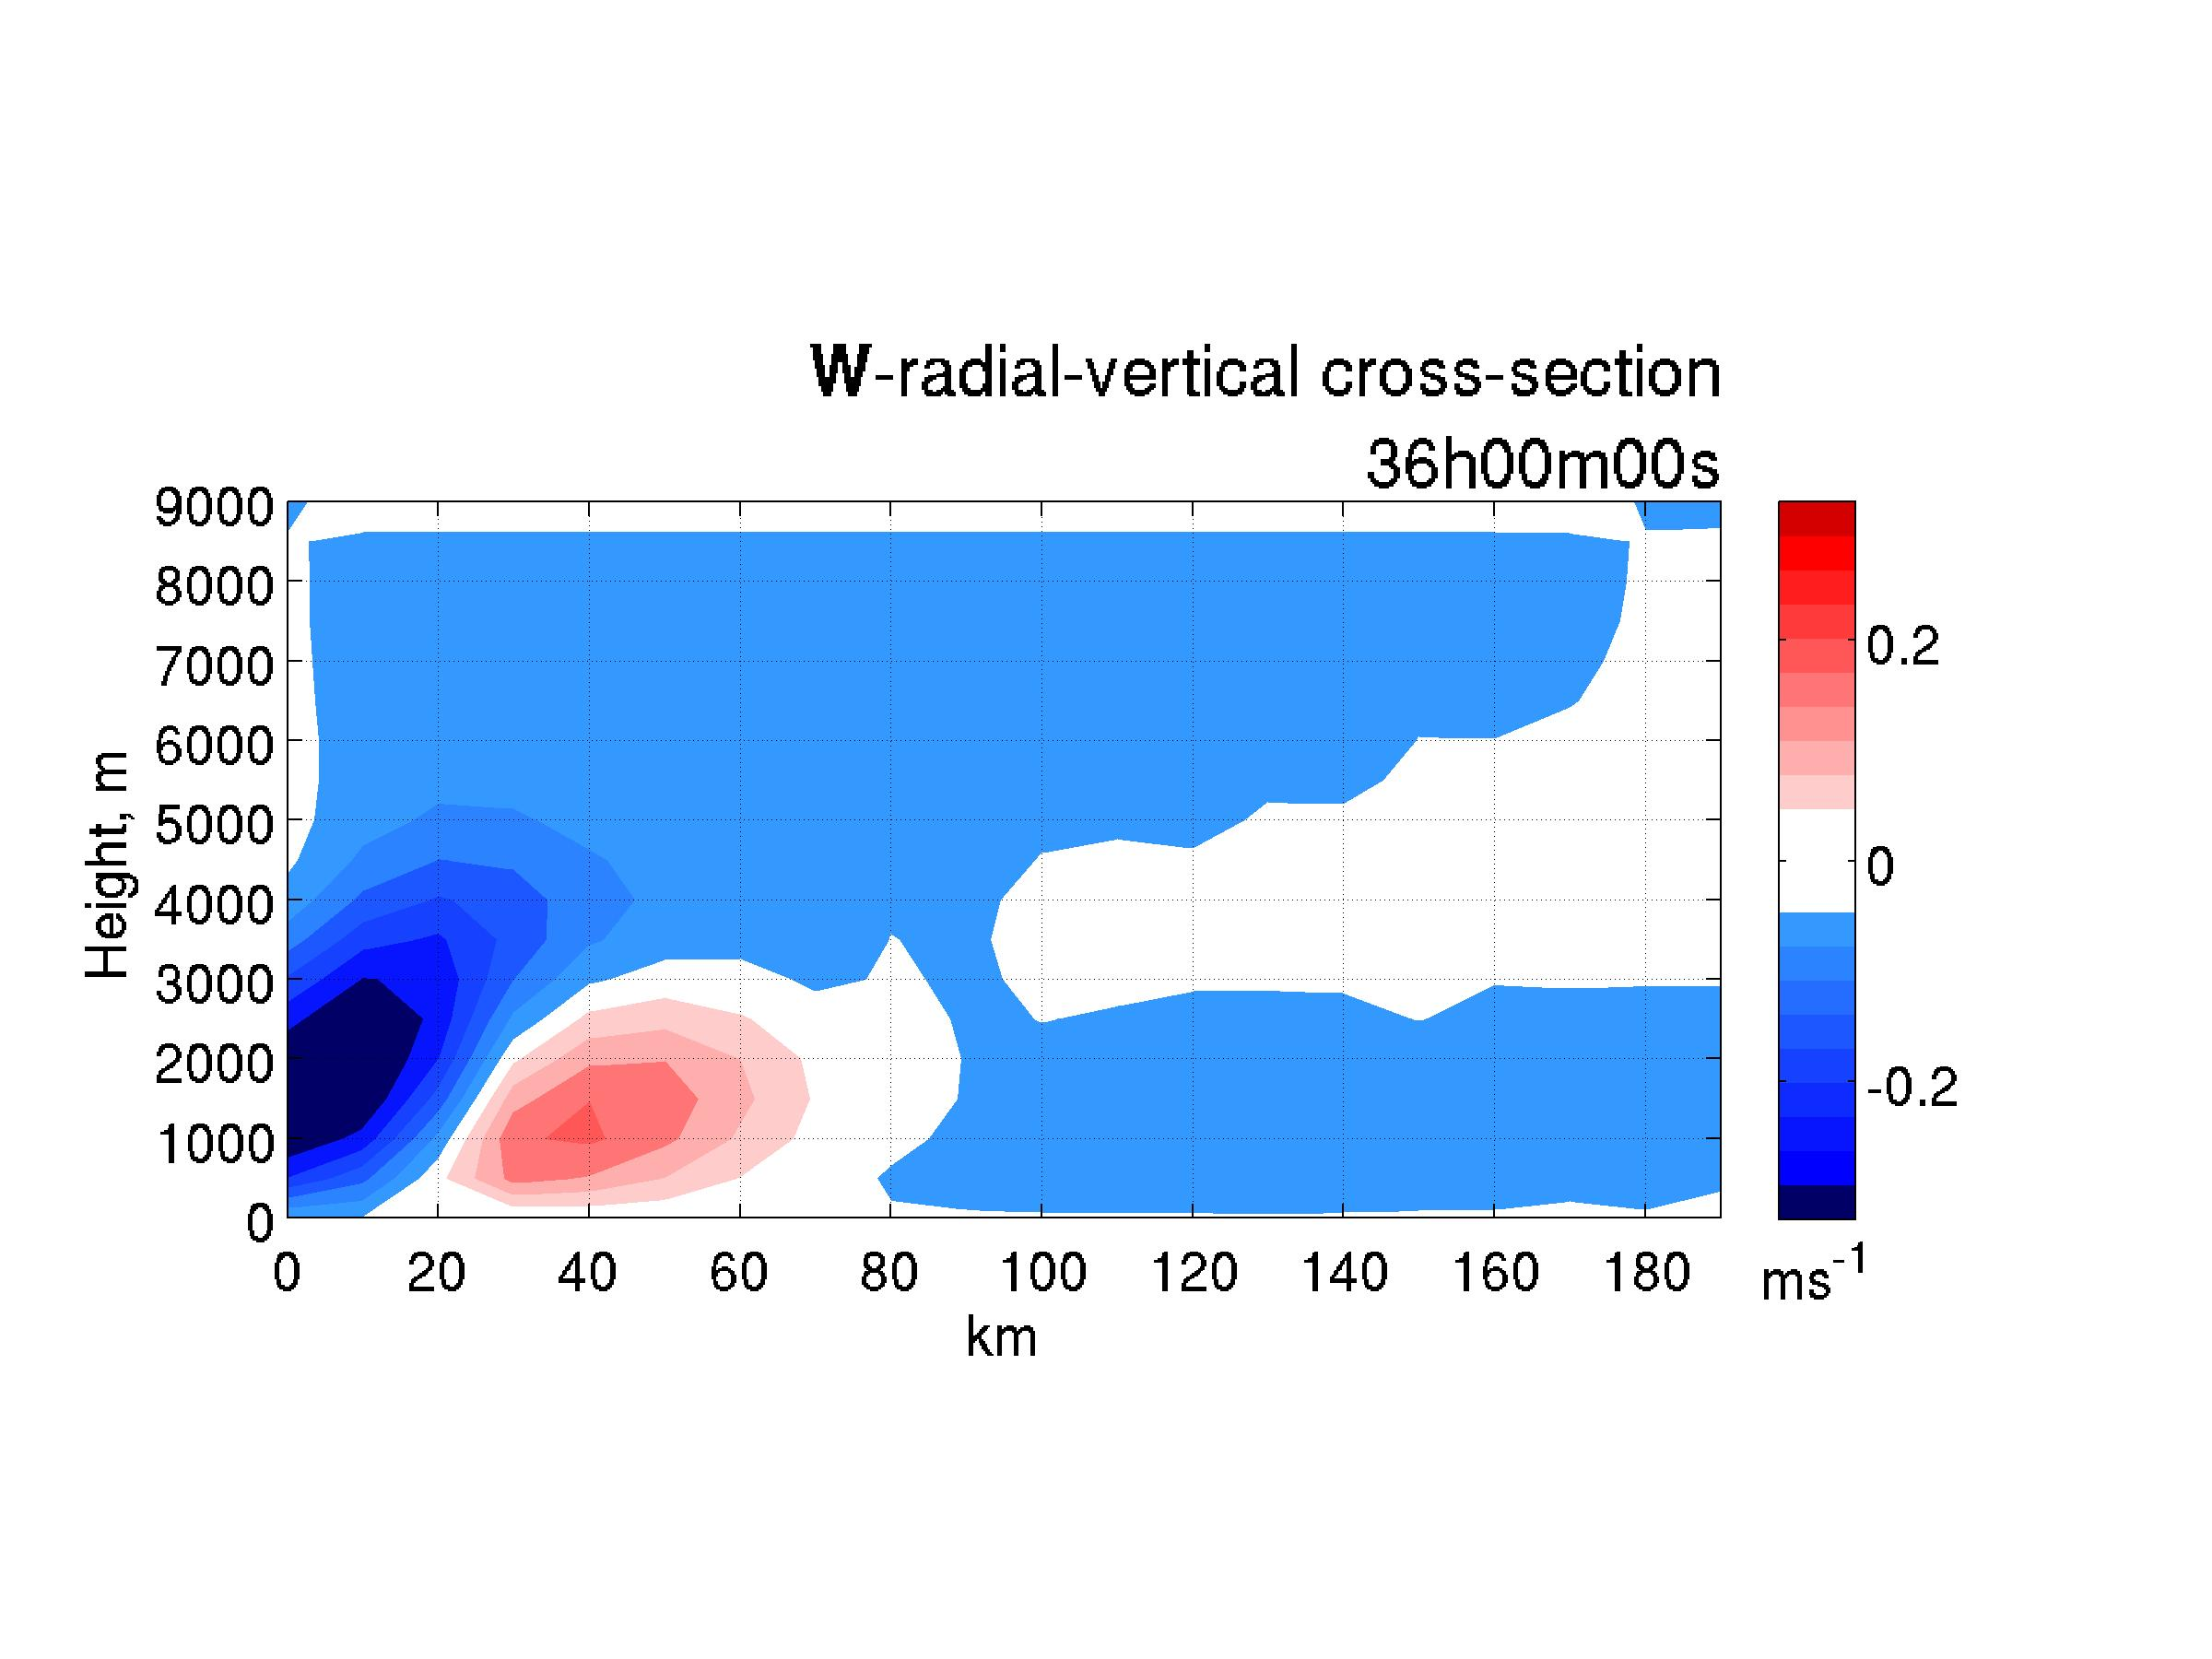
\includegraphics[width=\linewidth]{{./chapters/figures_results/ctrl_fields/w_rz_z.ix52.360000}.jpg}
		\caption{Вертикальная компонента скорости ветра ($w$), $\mps$.}
		\label{fig:ctrl_w_rz}
	\end{subfigure}
	\hfill
	\begin{subfigure}[t]{0.45\textwidth}
		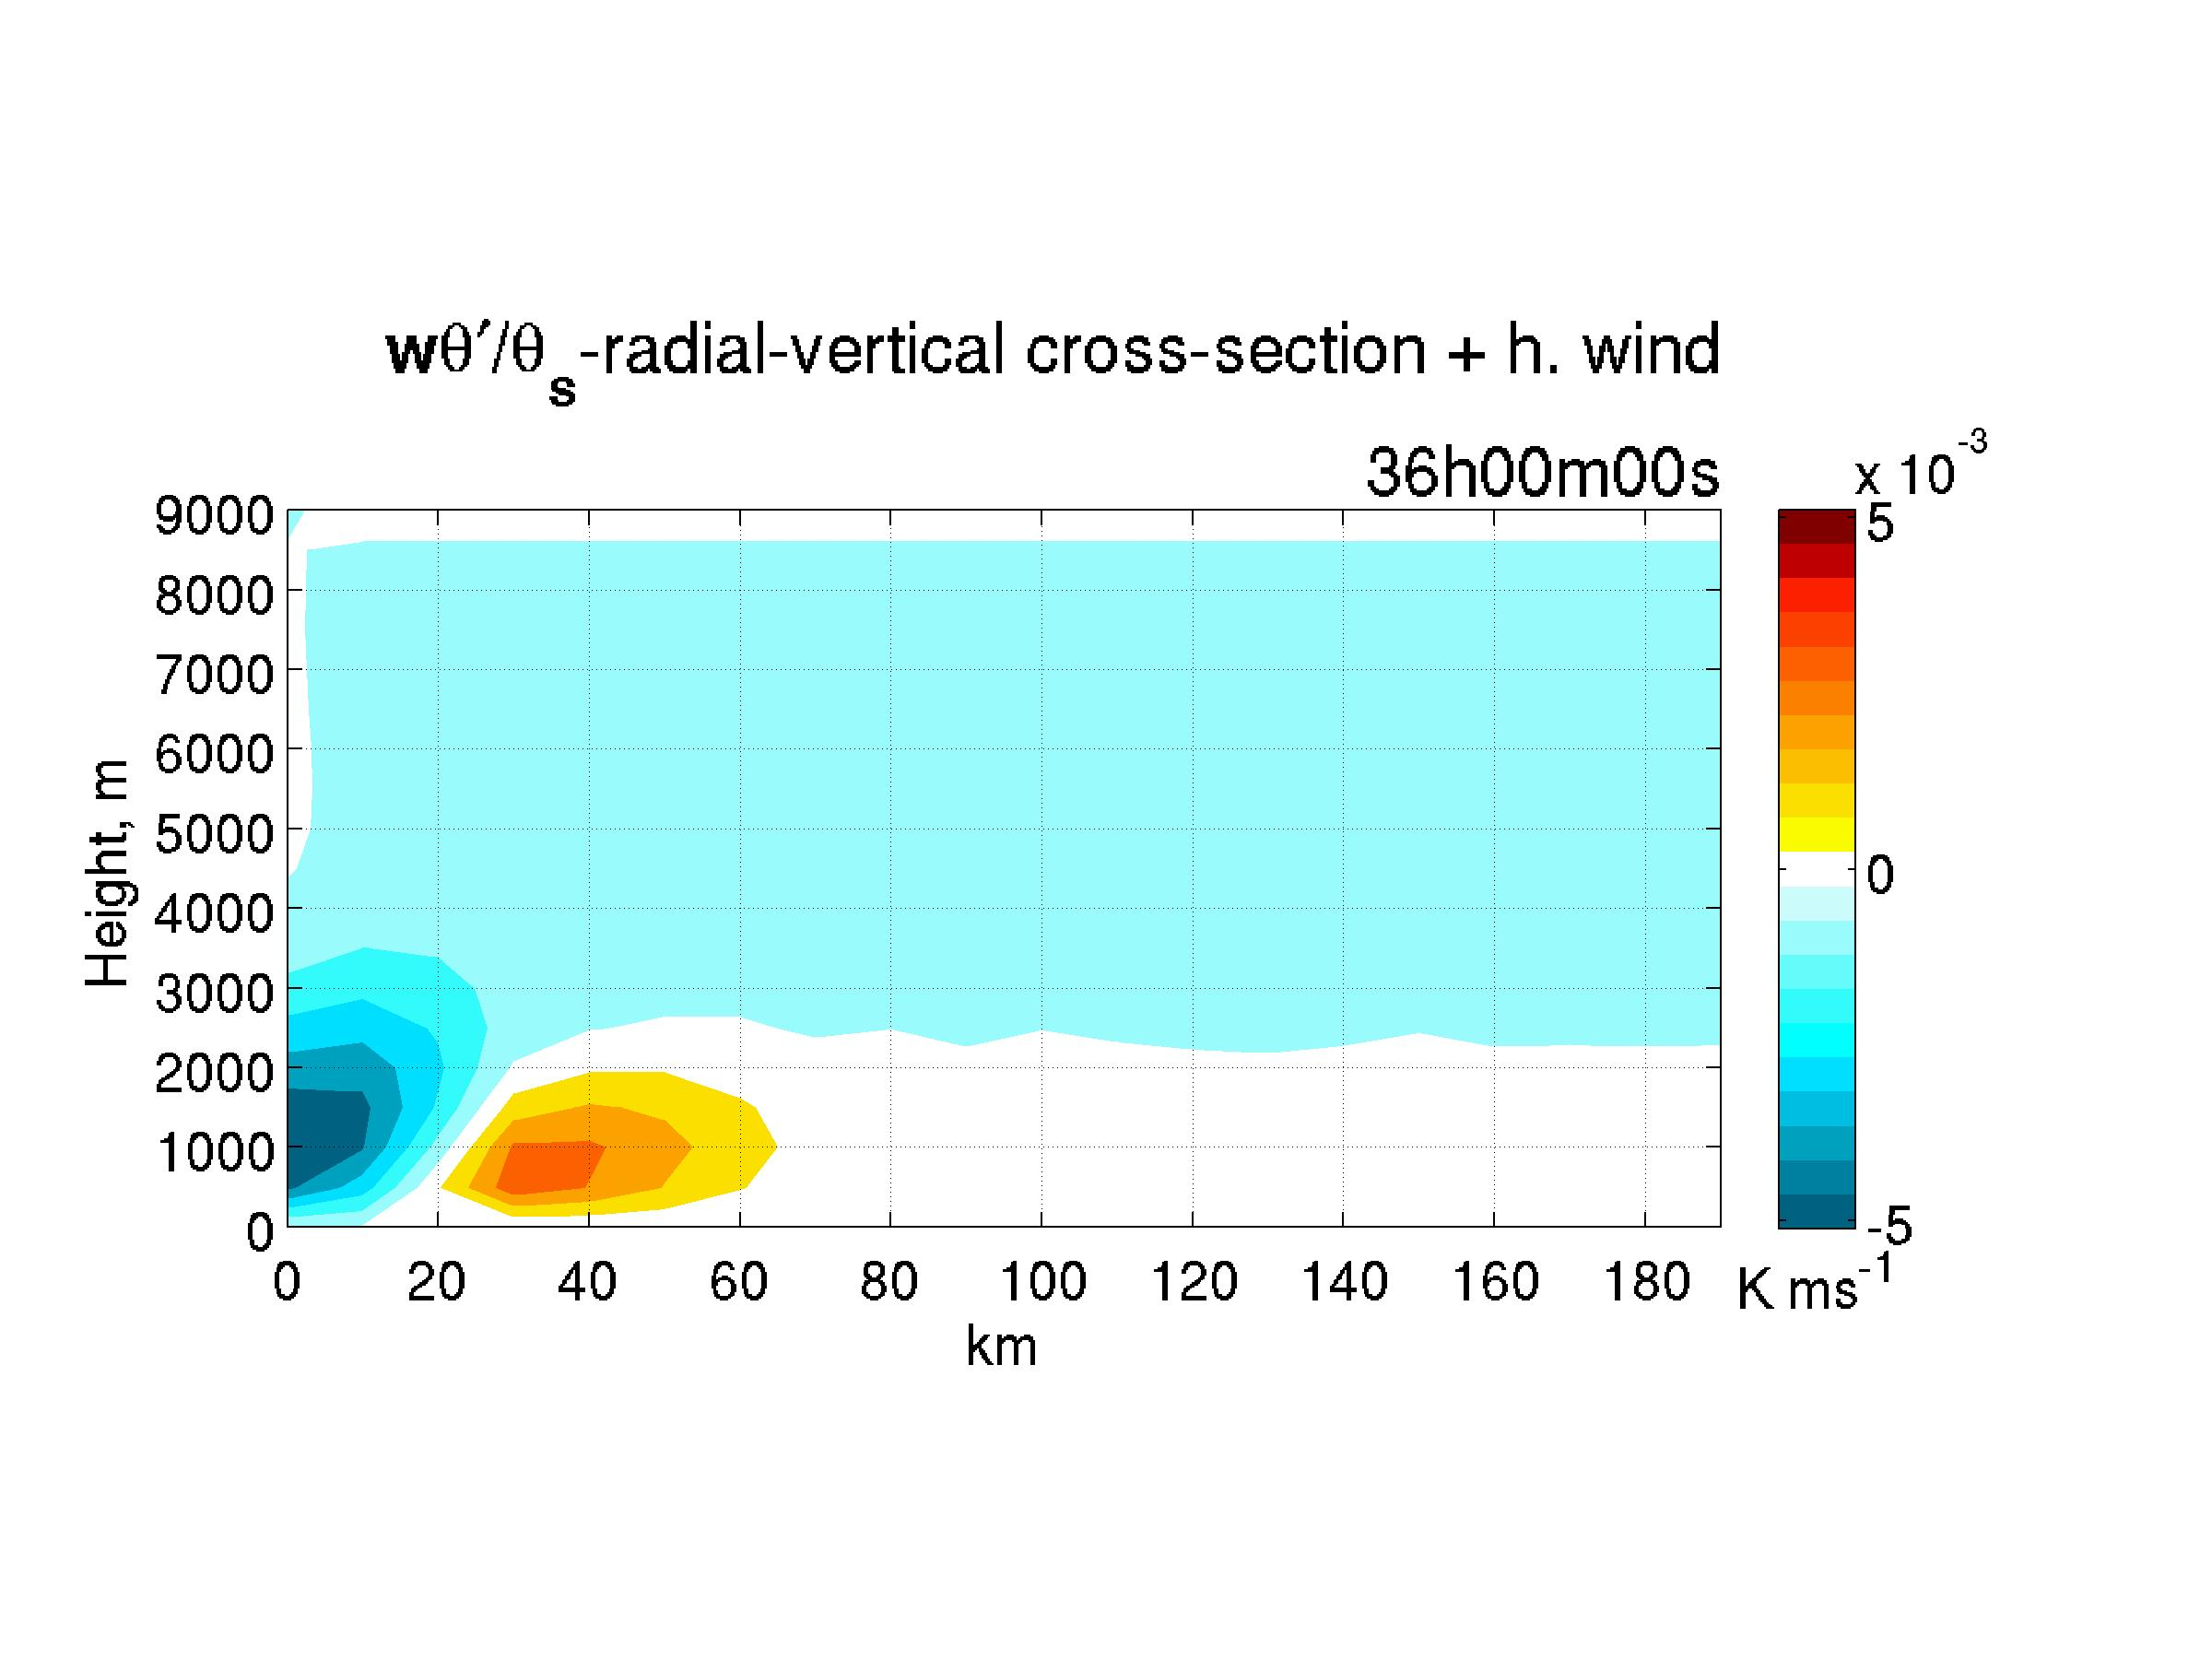
\includegraphics[width=\linewidth]{{./chapters/figures_results/ctrl_fields/buoyterm_rz_z.ix52.360000}.jpg}
		\caption{Поток силы плавучести ($w\theta'/\theta_s$), $\mps$.}
		\label{fig:ctrl_buoy_rz}
	\end{subfigure}
	\hfill
	\begin{subfigure}[t]{0.45\textwidth}
		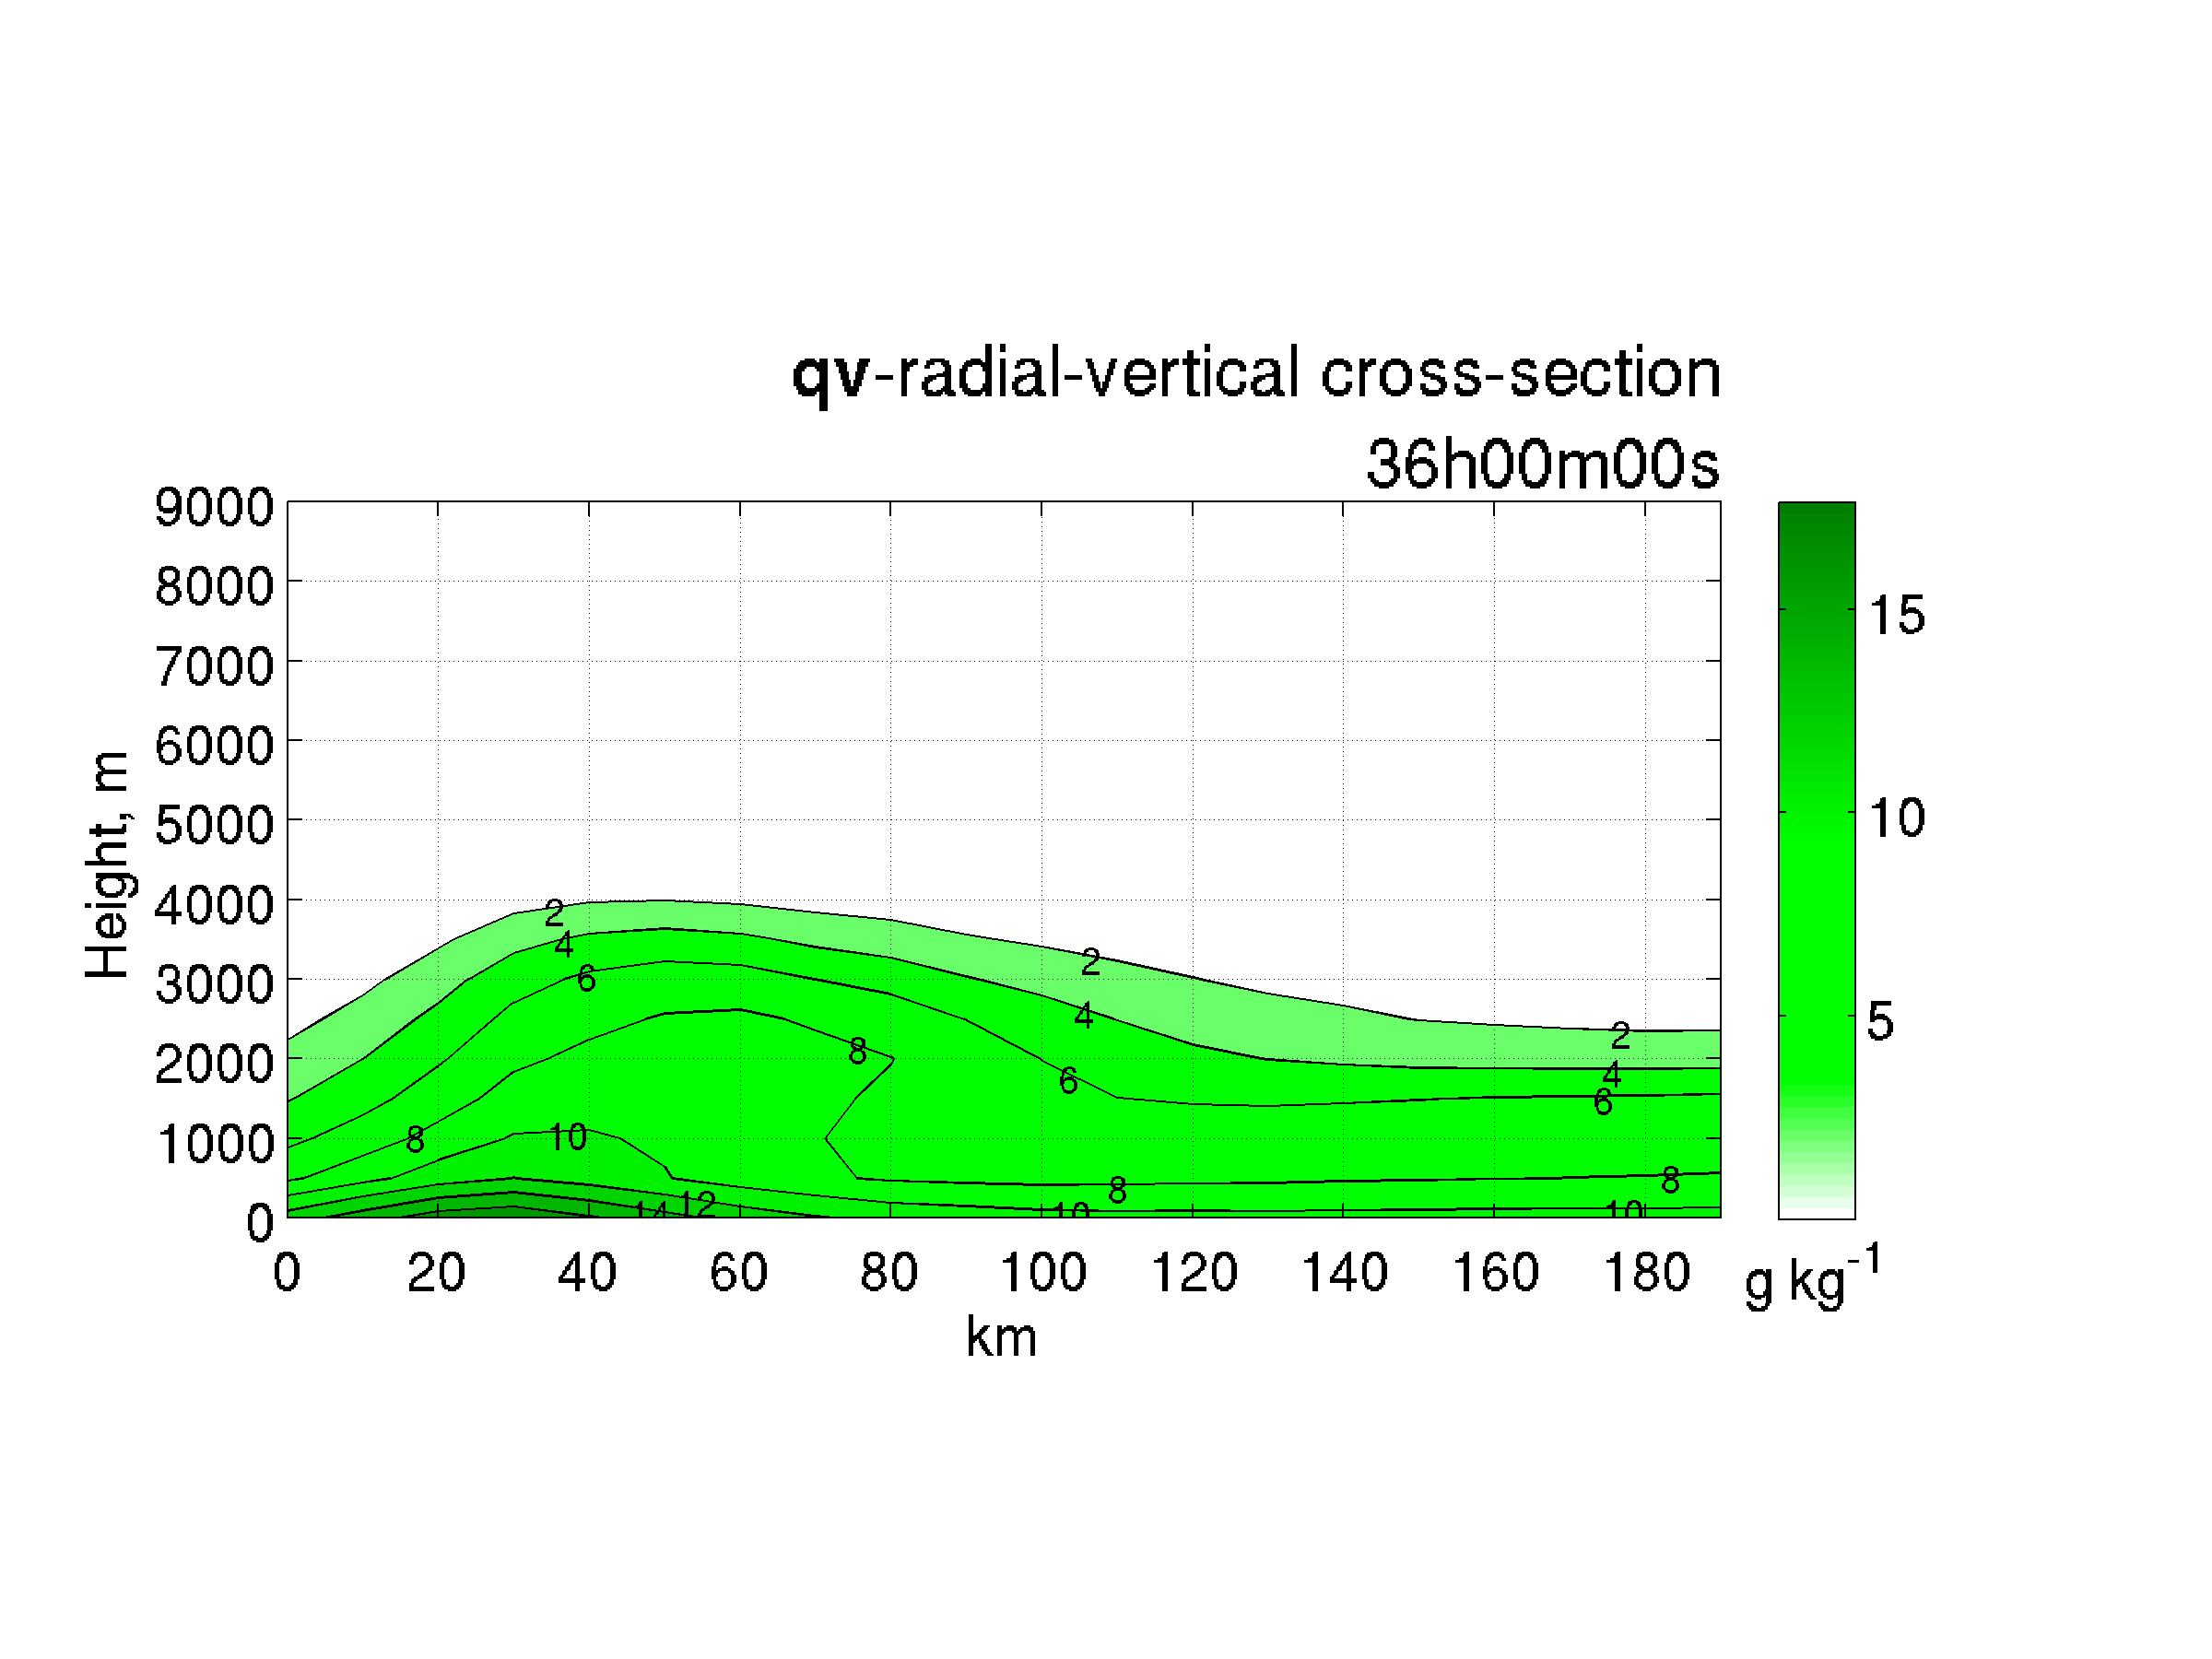
\includegraphics[width=\linewidth]{{./chapters/figures_results/ctrl_fields/qv_rz_z.ix52.360000}.jpg}
		\caption{Удельная влажность ($q_v$), $\gpkg$.}
		\label{fig:ctrl_qv_rz}
	\end{subfigure}
    \caption{Радиально-вертикальные разрезы. По оси абсцисс отложен радиус, $\km$, по оси ординат --- высота, $\m$. Эксперимент CTRL. 36 час модельного времени.}
\end{figure}

Под действием силы барического градиента в центре области возникает конвергенция скорости, которая под действием силы вращения Земли приобретает циклоническую завихренность (\ref{fig:ctrl_vort_rz}). Адекватность воспроизведения моделью этого фундаментального явления было проверено в дополнительном эксперименте с отключенным ускорением Кориолиса в уравнении движения (\ref{eq:progn1,eq:progn2}). Как видно из рис. \ref{fig:ctrl_vrvt_rz}, где изображены радиальная и азимутальная (тангенциальная) скорости, в стадии развитого вихря конвергенция сосредоточена ниже $1000\m$ на расстоянии от $40$ до $120\km$ с максимумом вблизи земной поверхности и на радиусе $50\km$. Внутреннюю часть этой зоны обозначим как глаз циклона в соответствии с терминологией тропических циклонов. Выше зоны конвергенции находится менее интенсивная область оттока воздуха, характеризующаяся положительной радиальной скоростью.

На рис. \ref{fig:ctrl_vrvt_rz} черным цветом показаны изолинии азимутальной скорости движения воздуха в вихре. Максимум циклонического азимутального ветра находится на уровне нулевой радиальной скорости ($500$--$1000\m$) и составляет $11.9\mps$, а радиус максимальных значений равняется около $40\km$ (радиус максимального ветра, РМВ). Существовавший в начальные этапы развития циклона слабый высотный антициклон уже не виден в 36 час модельного времени. Глазу циклона соответствует область малых скоростей ветра. Заметим, что глаз вихря оказывается слишком малым в поперечнике, чем обычно характерно для полярных мезоциклонов (\citep{CraigGray1996}).

Радиальный разрез вертикальной скорости виден на рис. \ref{fig:ctrl_w_rz}. Распределение этой компоненты ветра таково, что область положительных значений находится на расстоянии $20$--$70\km$ от центра циклона и наклонена \emph{от} центра. То есть область $w>0$ совпадает с областью максимальных ветров. Восходящие движения наиболее сильны в слое $1000$--$1500\m$ над поверхностью, где $w$ достигает $0.2\mps$. Отрицательные значения вертикальной скорости наблюдаются в области глаза циклона, и по амплитуде превосходят положительные в $\approx 1.5$ раза. 

Относительная завихренность в нижних слоях атмосферы распределена симметрично относительно центра циклона, причем максимум, уже на порядок превосходящий параметр Кориолиса, наблюдается на расстоянии около $25\km$ от центра. Среди членов, определяющих  изменение завихренности наибольшую величину имеет слагаемое растяжения (\ref{fig:ctrl_stretch36}), причем положительные значения находятся на периферии циклона ($\approx 2\times 10^{-7}\s^{-2}$), а отрицательные --- в центре. Таким образом, проявляется тенденция к расширению циклона и концентрации количества движения на кольце максимальных ветров. Вторым по значимости в бюджете завихренности является слагаемое горизонтальной адвекции (порядка $10^{-7}$), у которого преобладают отрицательные значения, несколько компенсируя дивергентное слагаемое на внешнем радиусе циклона. Два остальных компонента бюджета завихренности имеют значения одного порядка ($10^{-8}$), но действуют противоположно: слагаемое вертикальной адвекции имеет отрицательные значения в рассматриваемом районе, а слагаемое наклона положительно.

\begin{figure}[t]
	\centering
	\begin{subfigure}[t]{0.45\textwidth}
		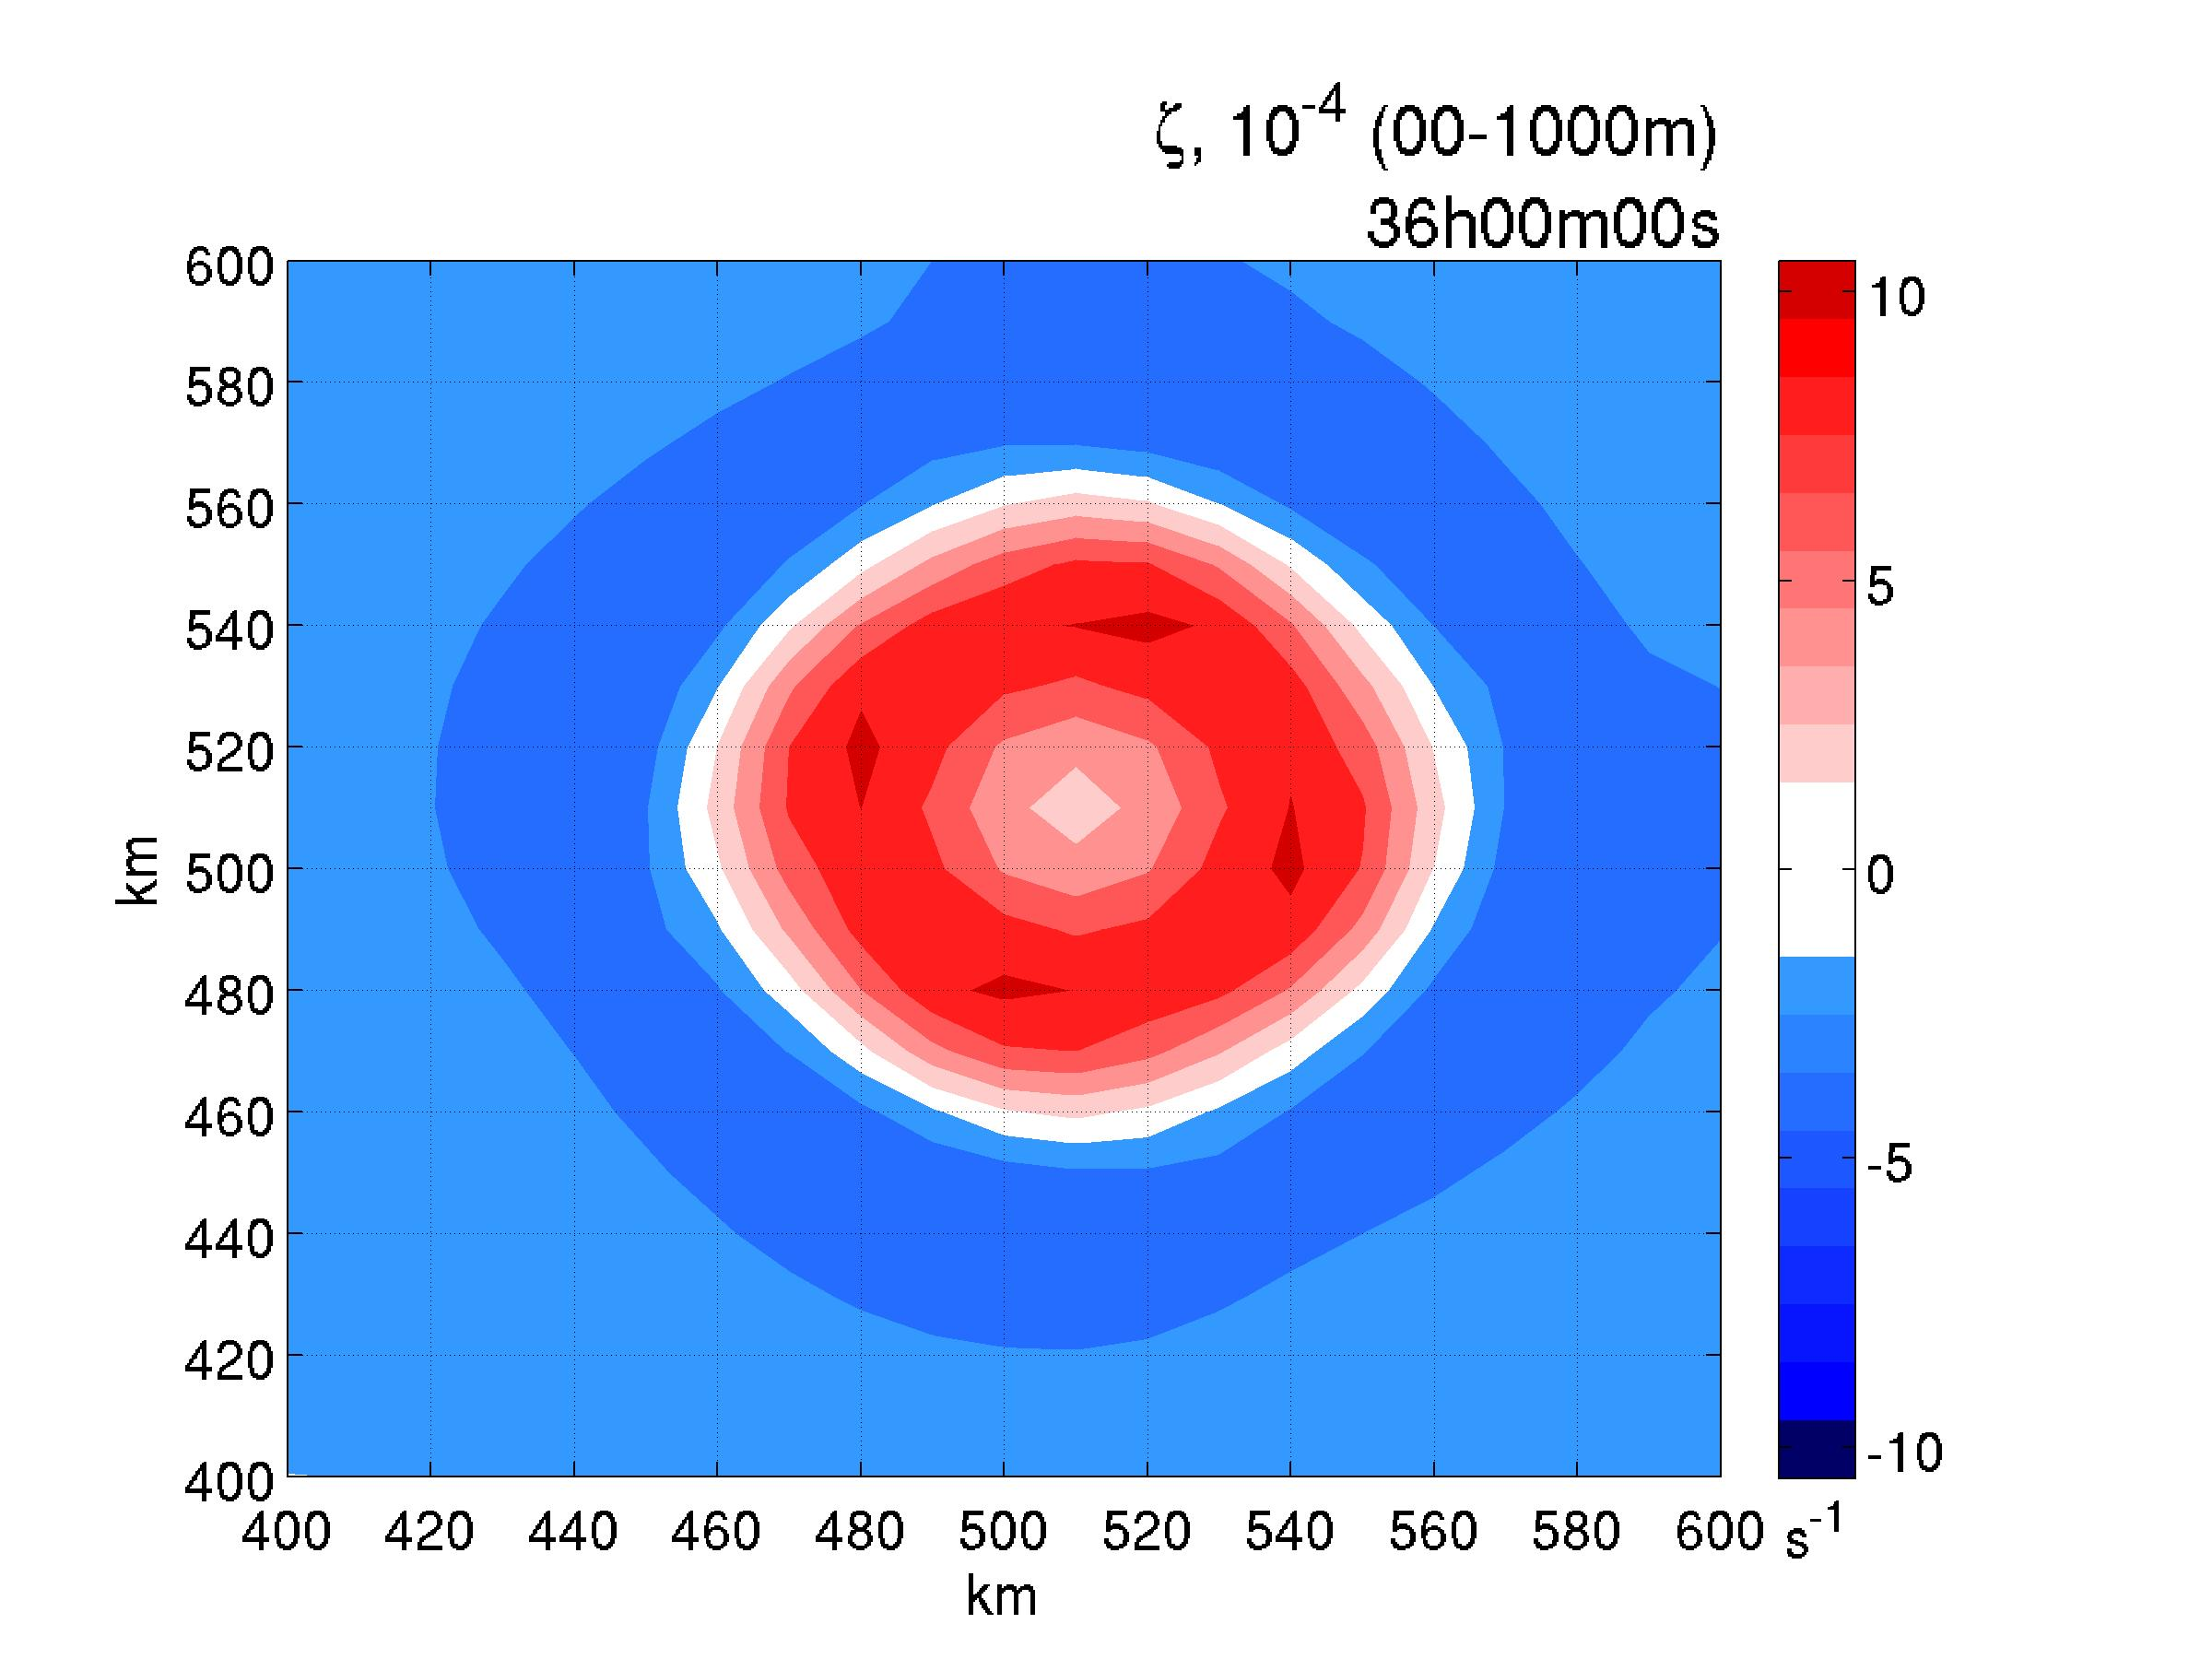
\includegraphics[width=\linewidth]{{./chapters/figures_results/ctrl_fields/rot_z_z.x41-x61.y41-y61.ilev02.360000}.jpg}
		\caption{ }
        \label{fig:ctrl_rotz36}
	\end{subfigure}
	\hfill
	\begin{subfigure}[t]{0.45\textwidth}
		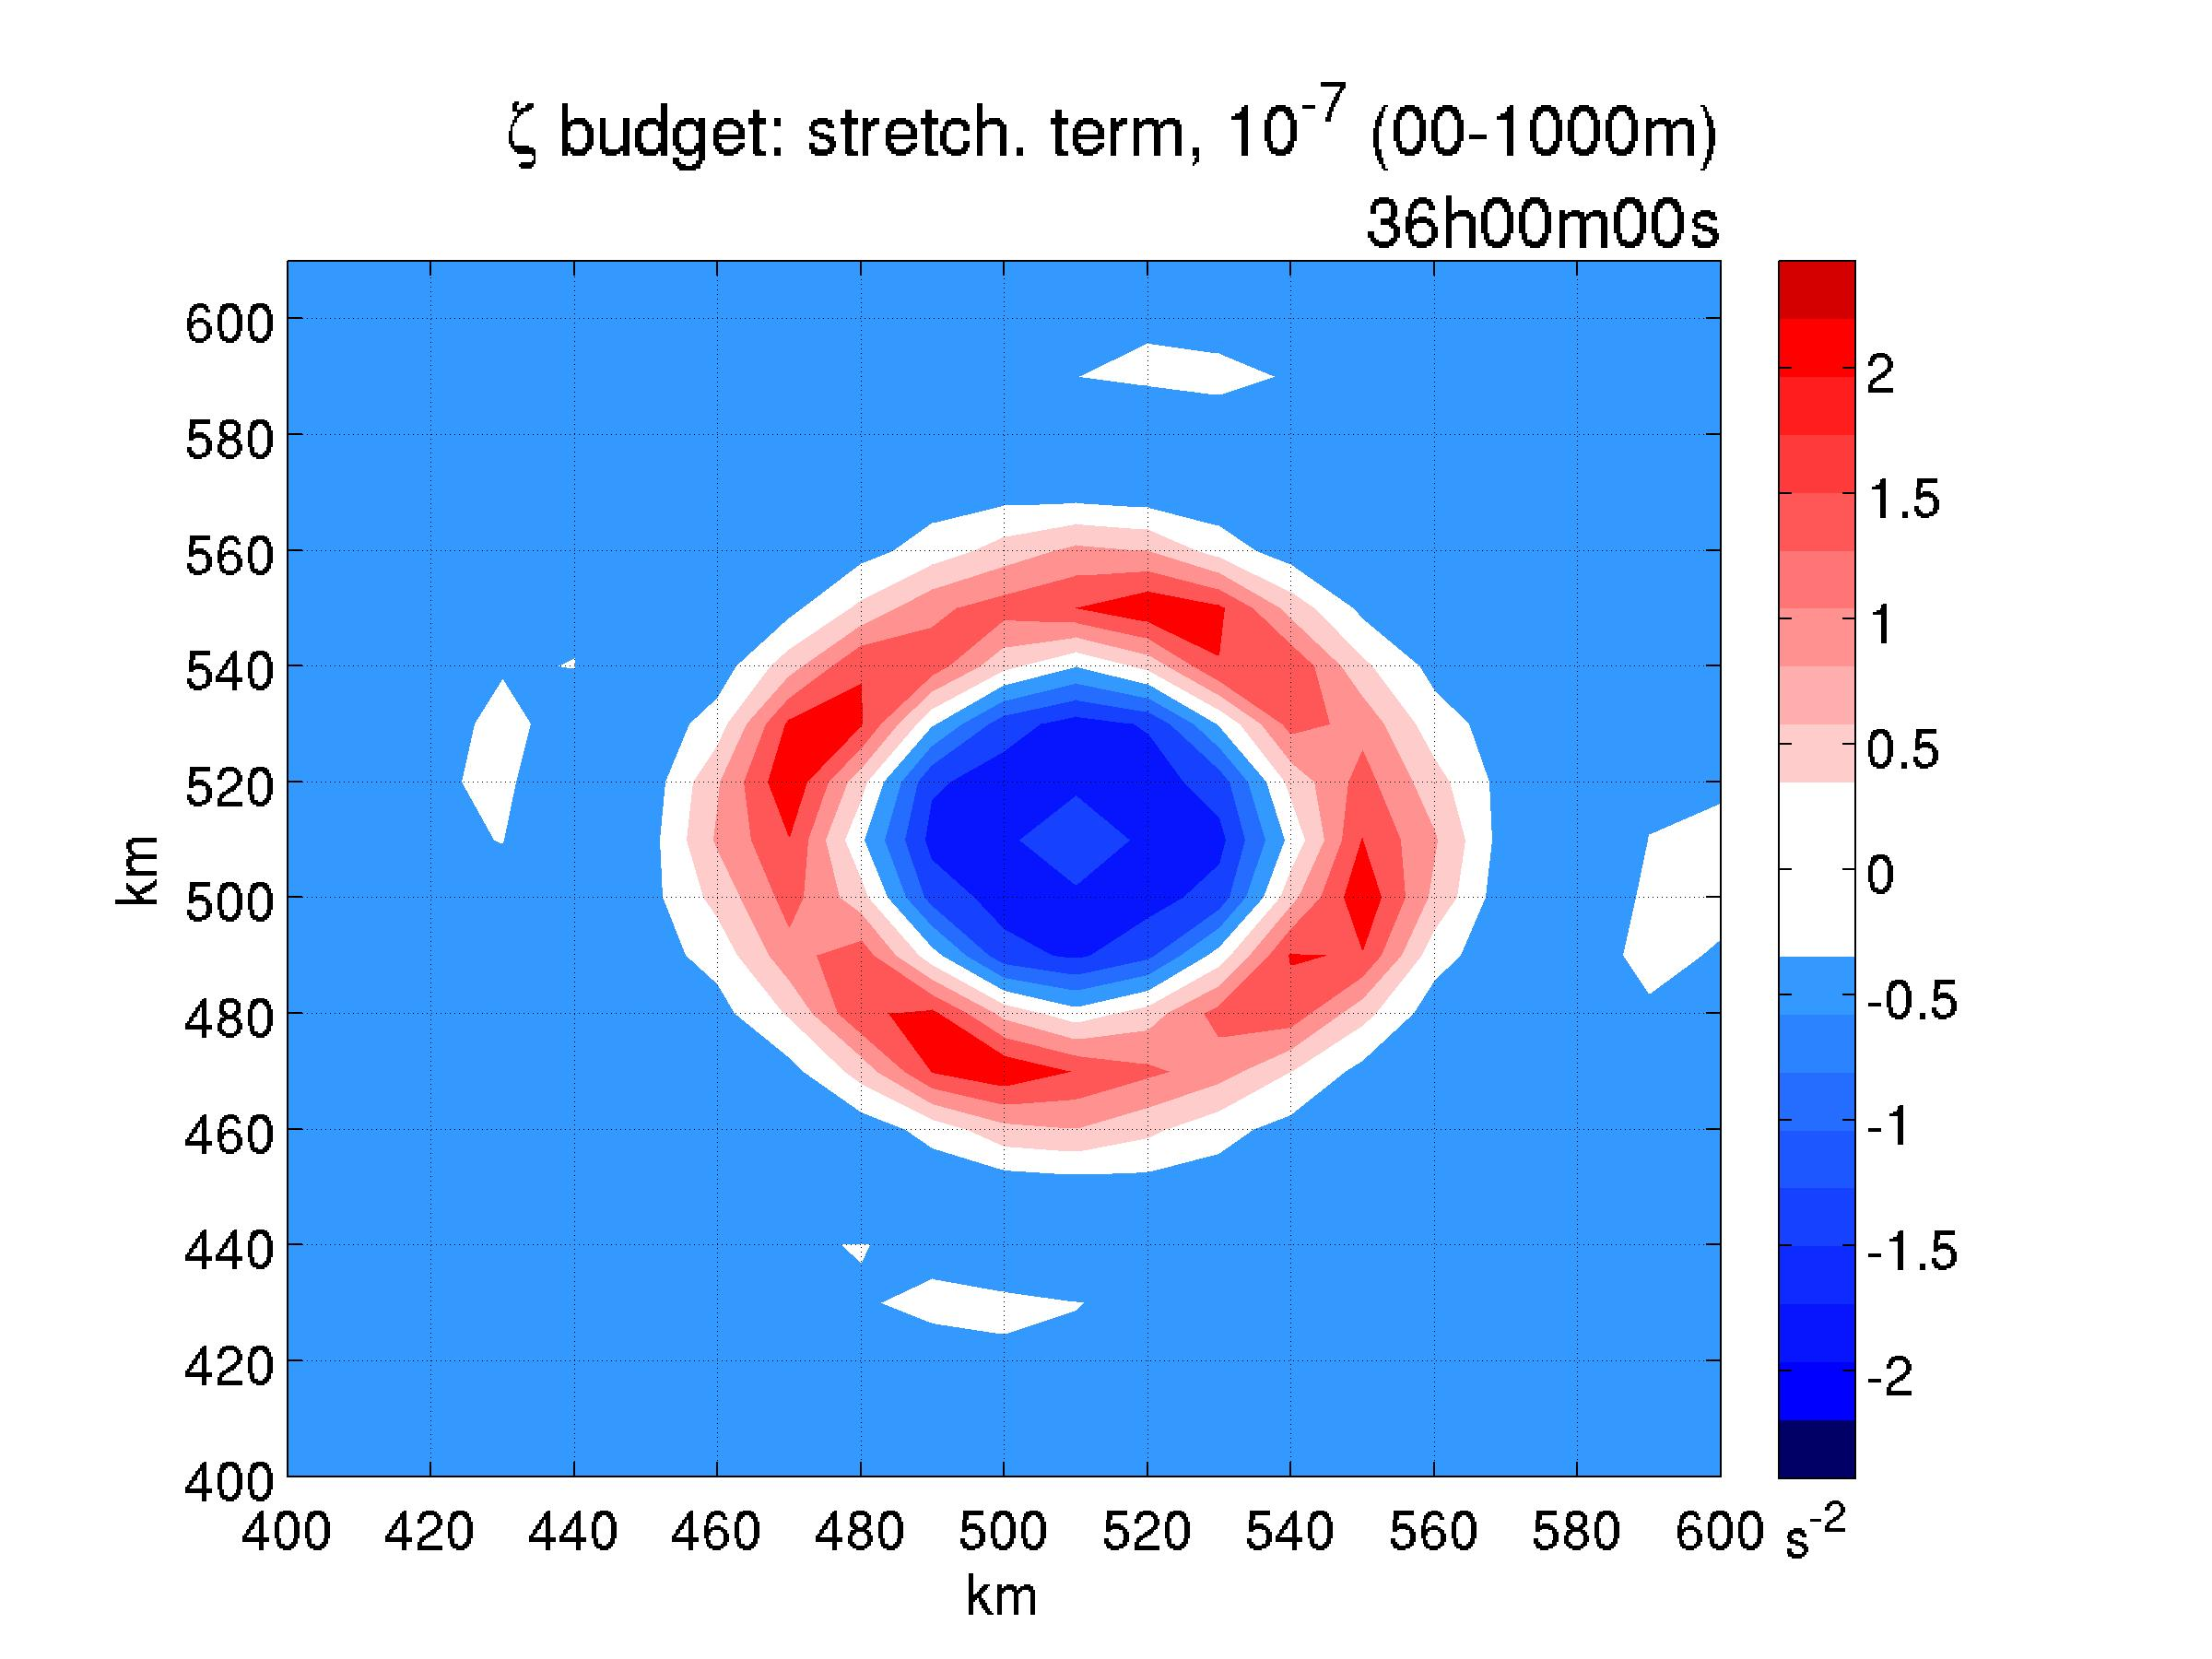
\includegraphics[width=\linewidth]{{./chapters/figures_results/ctrl_fields/vort_budget_stretch_z.x41-x62.y41-y61.ilev02.360000}.jpg}
		\caption{ }
		\label{fig:ctrl_stretch36}
	\end{subfigure}
    \caption{Поле относительной завихренности ($\zeta$) и слагаемое растяжения (\ref{eq:vorttend}) бюджета завихренности, осредненные в слое ниже $1000\m$. Эксперимент CTRL. 36 час модельного времени.}
\end{figure}

Развившийся вихрь находится в сбалансированном состоянии: правая и левая части в уравнении градиентного баланса (в котором слагаемое центростремительного ускорения превышает ускорение Кориолиса почти в 2 раза) очень близки по величине. Это также подтверждается рис. \ref{fig:grwindbal}.

\subsection{Разделение вихря}
Моделируемый мезоциклон достигает больших скоростей к концу вторых суток интегрирования, что вызывает численную неустойчивость эксперимента. При этом наблюдается разделение вихря на две отдельные циклонические депрессии (рис. \ref{fig:ctrl_split_hwind}), которые продолжают усиливаться, и в последний час эксперимента максимальная скорость ветра в нижней атмосфере превышает $80\mps$. 

\begin{wrapfigure}{L}{0.5\textwidth}
\begin{center}
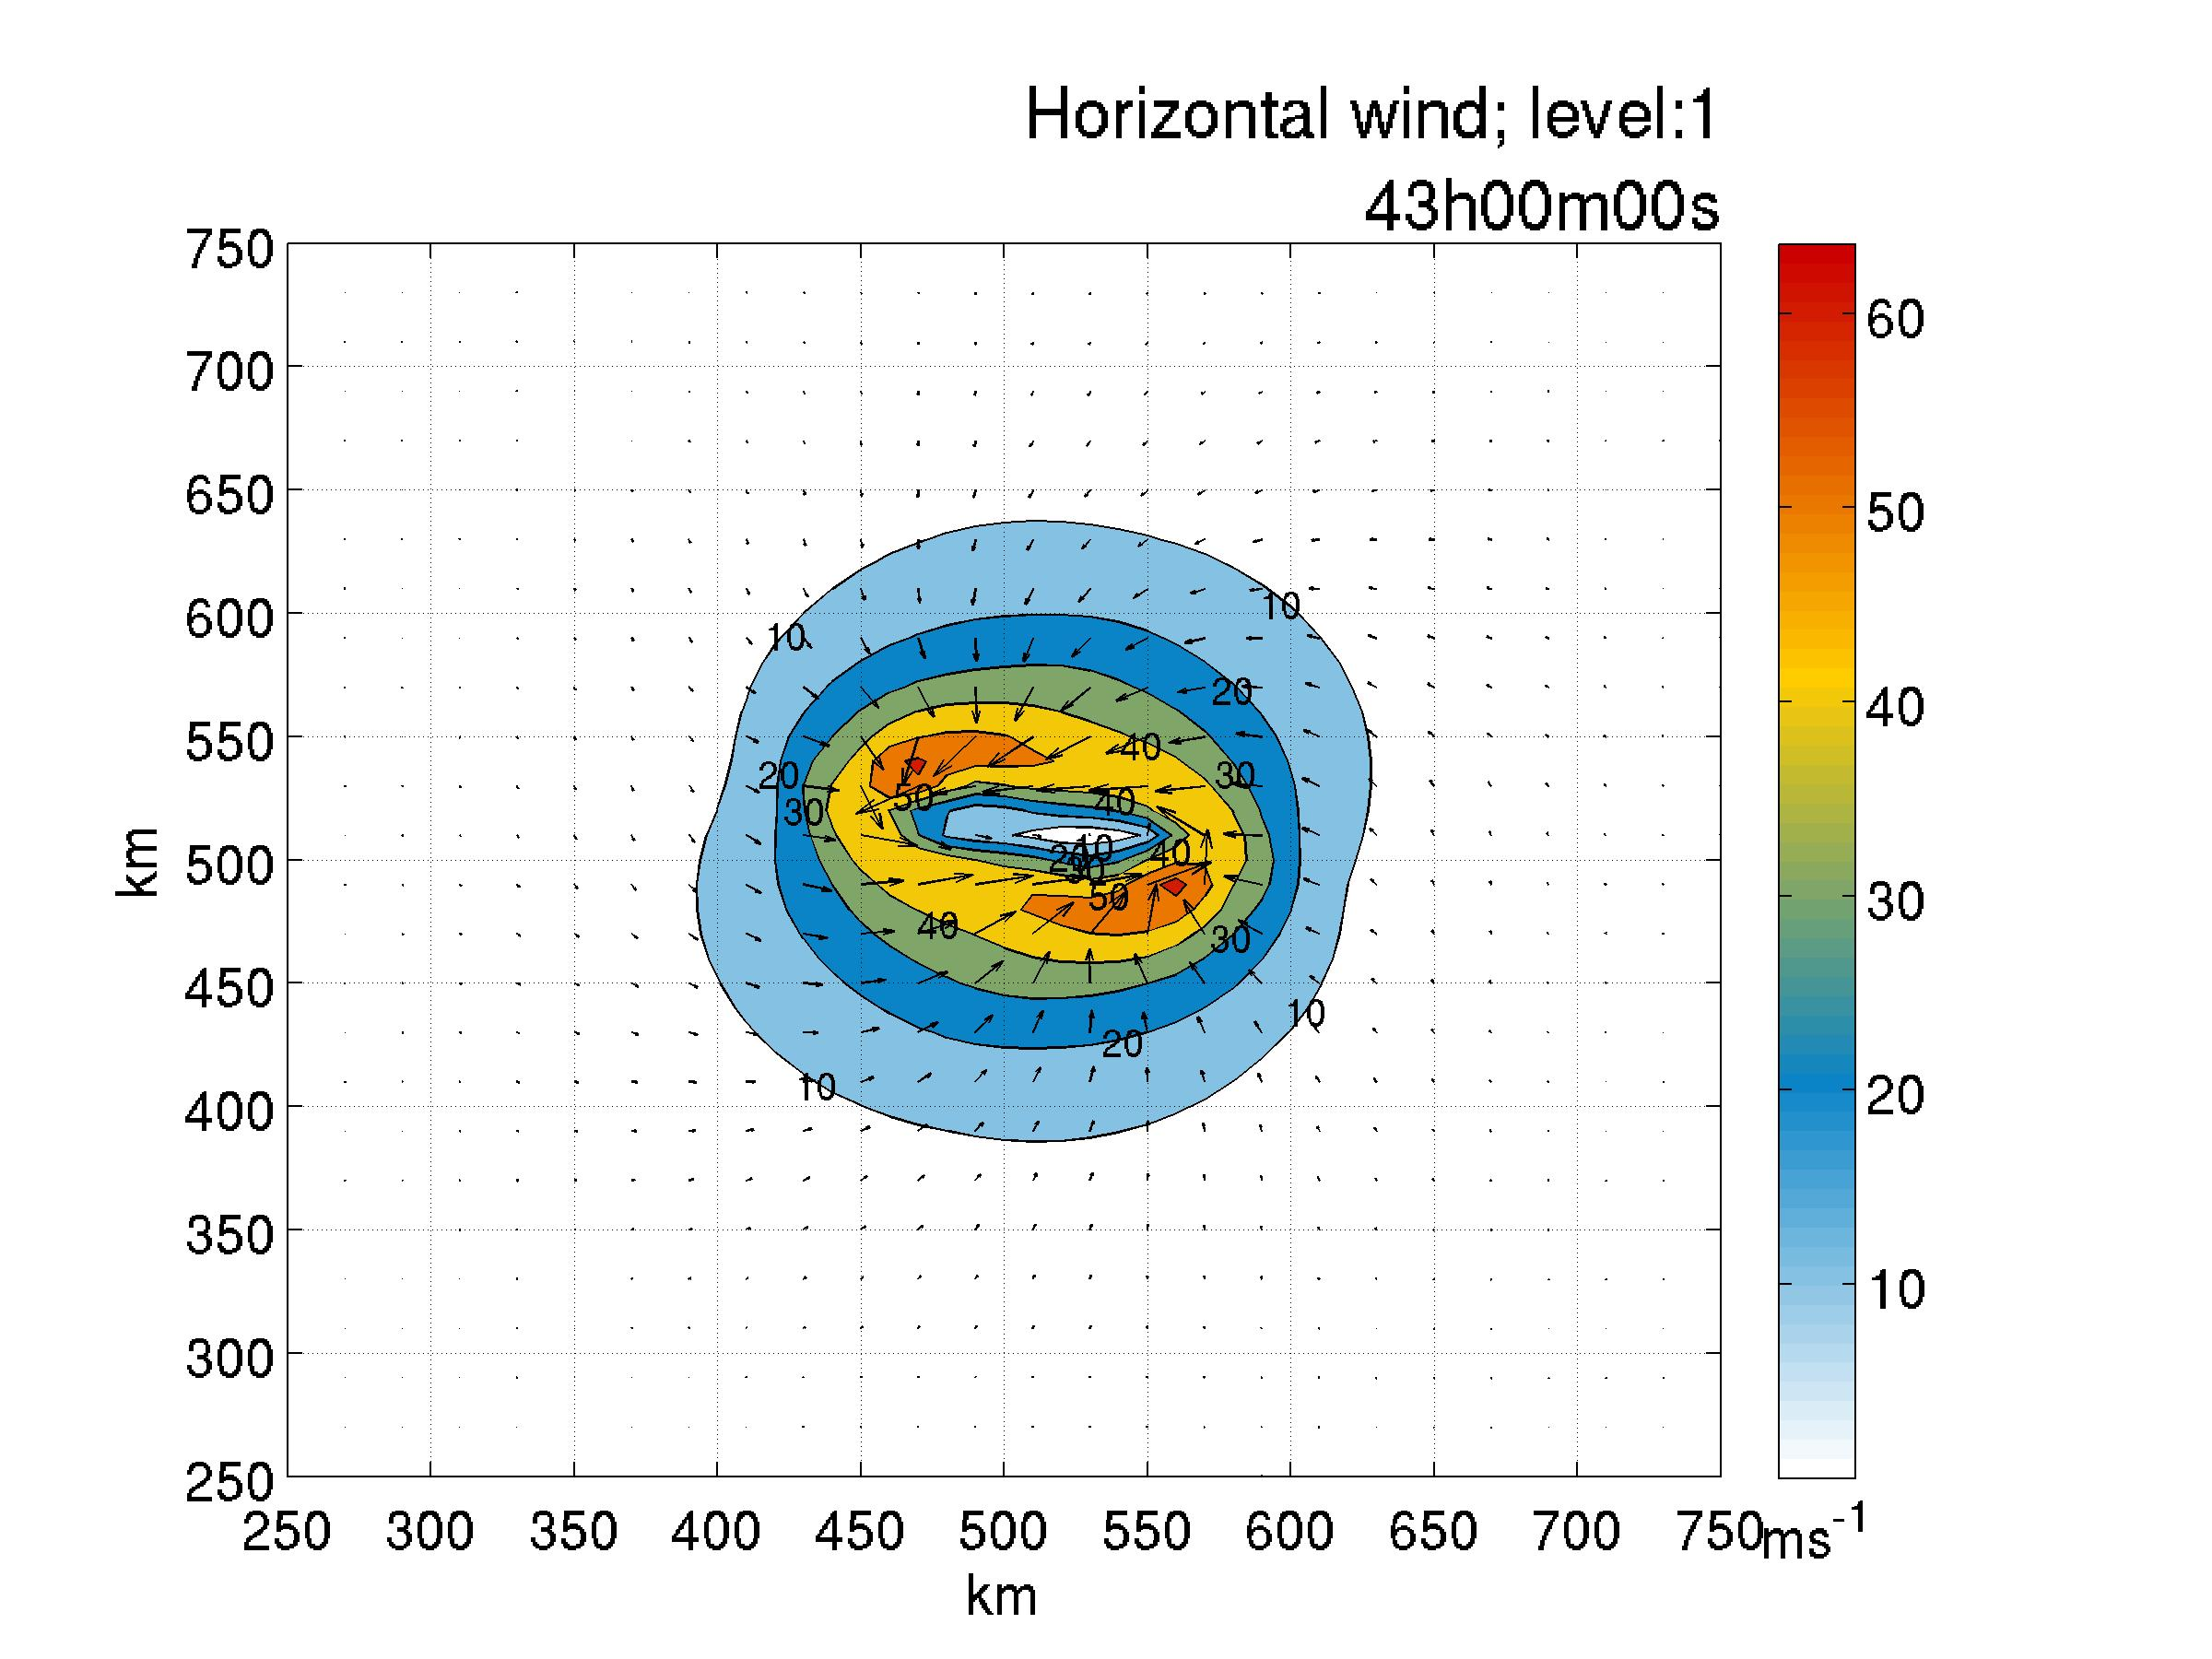
\includegraphics[width=\linewidth]{{./chapters/figures_results/ctrl_fields/VectorWind_z.x26-x76.y26-y76.ilev01.430000}.jpg}
\end{center}
\caption{Поле горизонтальной скорости ветра (фокус $500\times 500\km$). Эксперимент CTRL. 43 час модельного времени.}
\label{fig:ctrl_split_hwind}
\end{wrapfigure} 

В этом контексте был проведен дополнительный эксперимент (не показано) на расчетной области большего размера и с меньшими ограниченими на допустимые скорости ветра. При этом центральное циклоническое возмущение сначала разделялось на две части, которые двигались в противоположные стороны и, в свою очередь, разделялись на две части, каждая из которых также делилась на две части, и так далее. При этом каждый раз вихри меньшего размера делили общую КЭ поровну и продолжали интенсифицироваться. 

Можно предположить, что разделение вихря --- это реализация прямого каскада энергии по спектру. Энергия 'накачивается' на узком диапазоне волновых чисел, соответствующих изолированному возмущению, а затем сбрасывается в более мелкие масштабы через разделение вихря. Для проверки этой гипотезы был построен спектр.....................

%\subsection{Энергетическая диагностика}
%Перейдем к анализу динамики возмущения с точки зрения энергетики атмосферы. На рис. \ref{fig:ctrlene} представлена эволюция интегральной кинетической энергии. В данном случае величина общей кинетической энергии и кинетической энергии возмущений, очевидно, совпадает, так как в модельной области развивается только рассматриваемый циклон. Сначала ход кинетической энергии испытывает колебание, связанное с испусканием инерционно-гравитационных волн. Затем она непрерывно растет до значений порядка $10\Jpm$, что согласуется с результатами идеализированного моделирования других авторов (например, \citep{YanaseNiino2007}). При этом скорость роста энергии даже больше, чем по экспоненциальной зависимости. 
%
%\begin{wrapfigure}{R}{0.5\textwidth}
%\begin{center}
%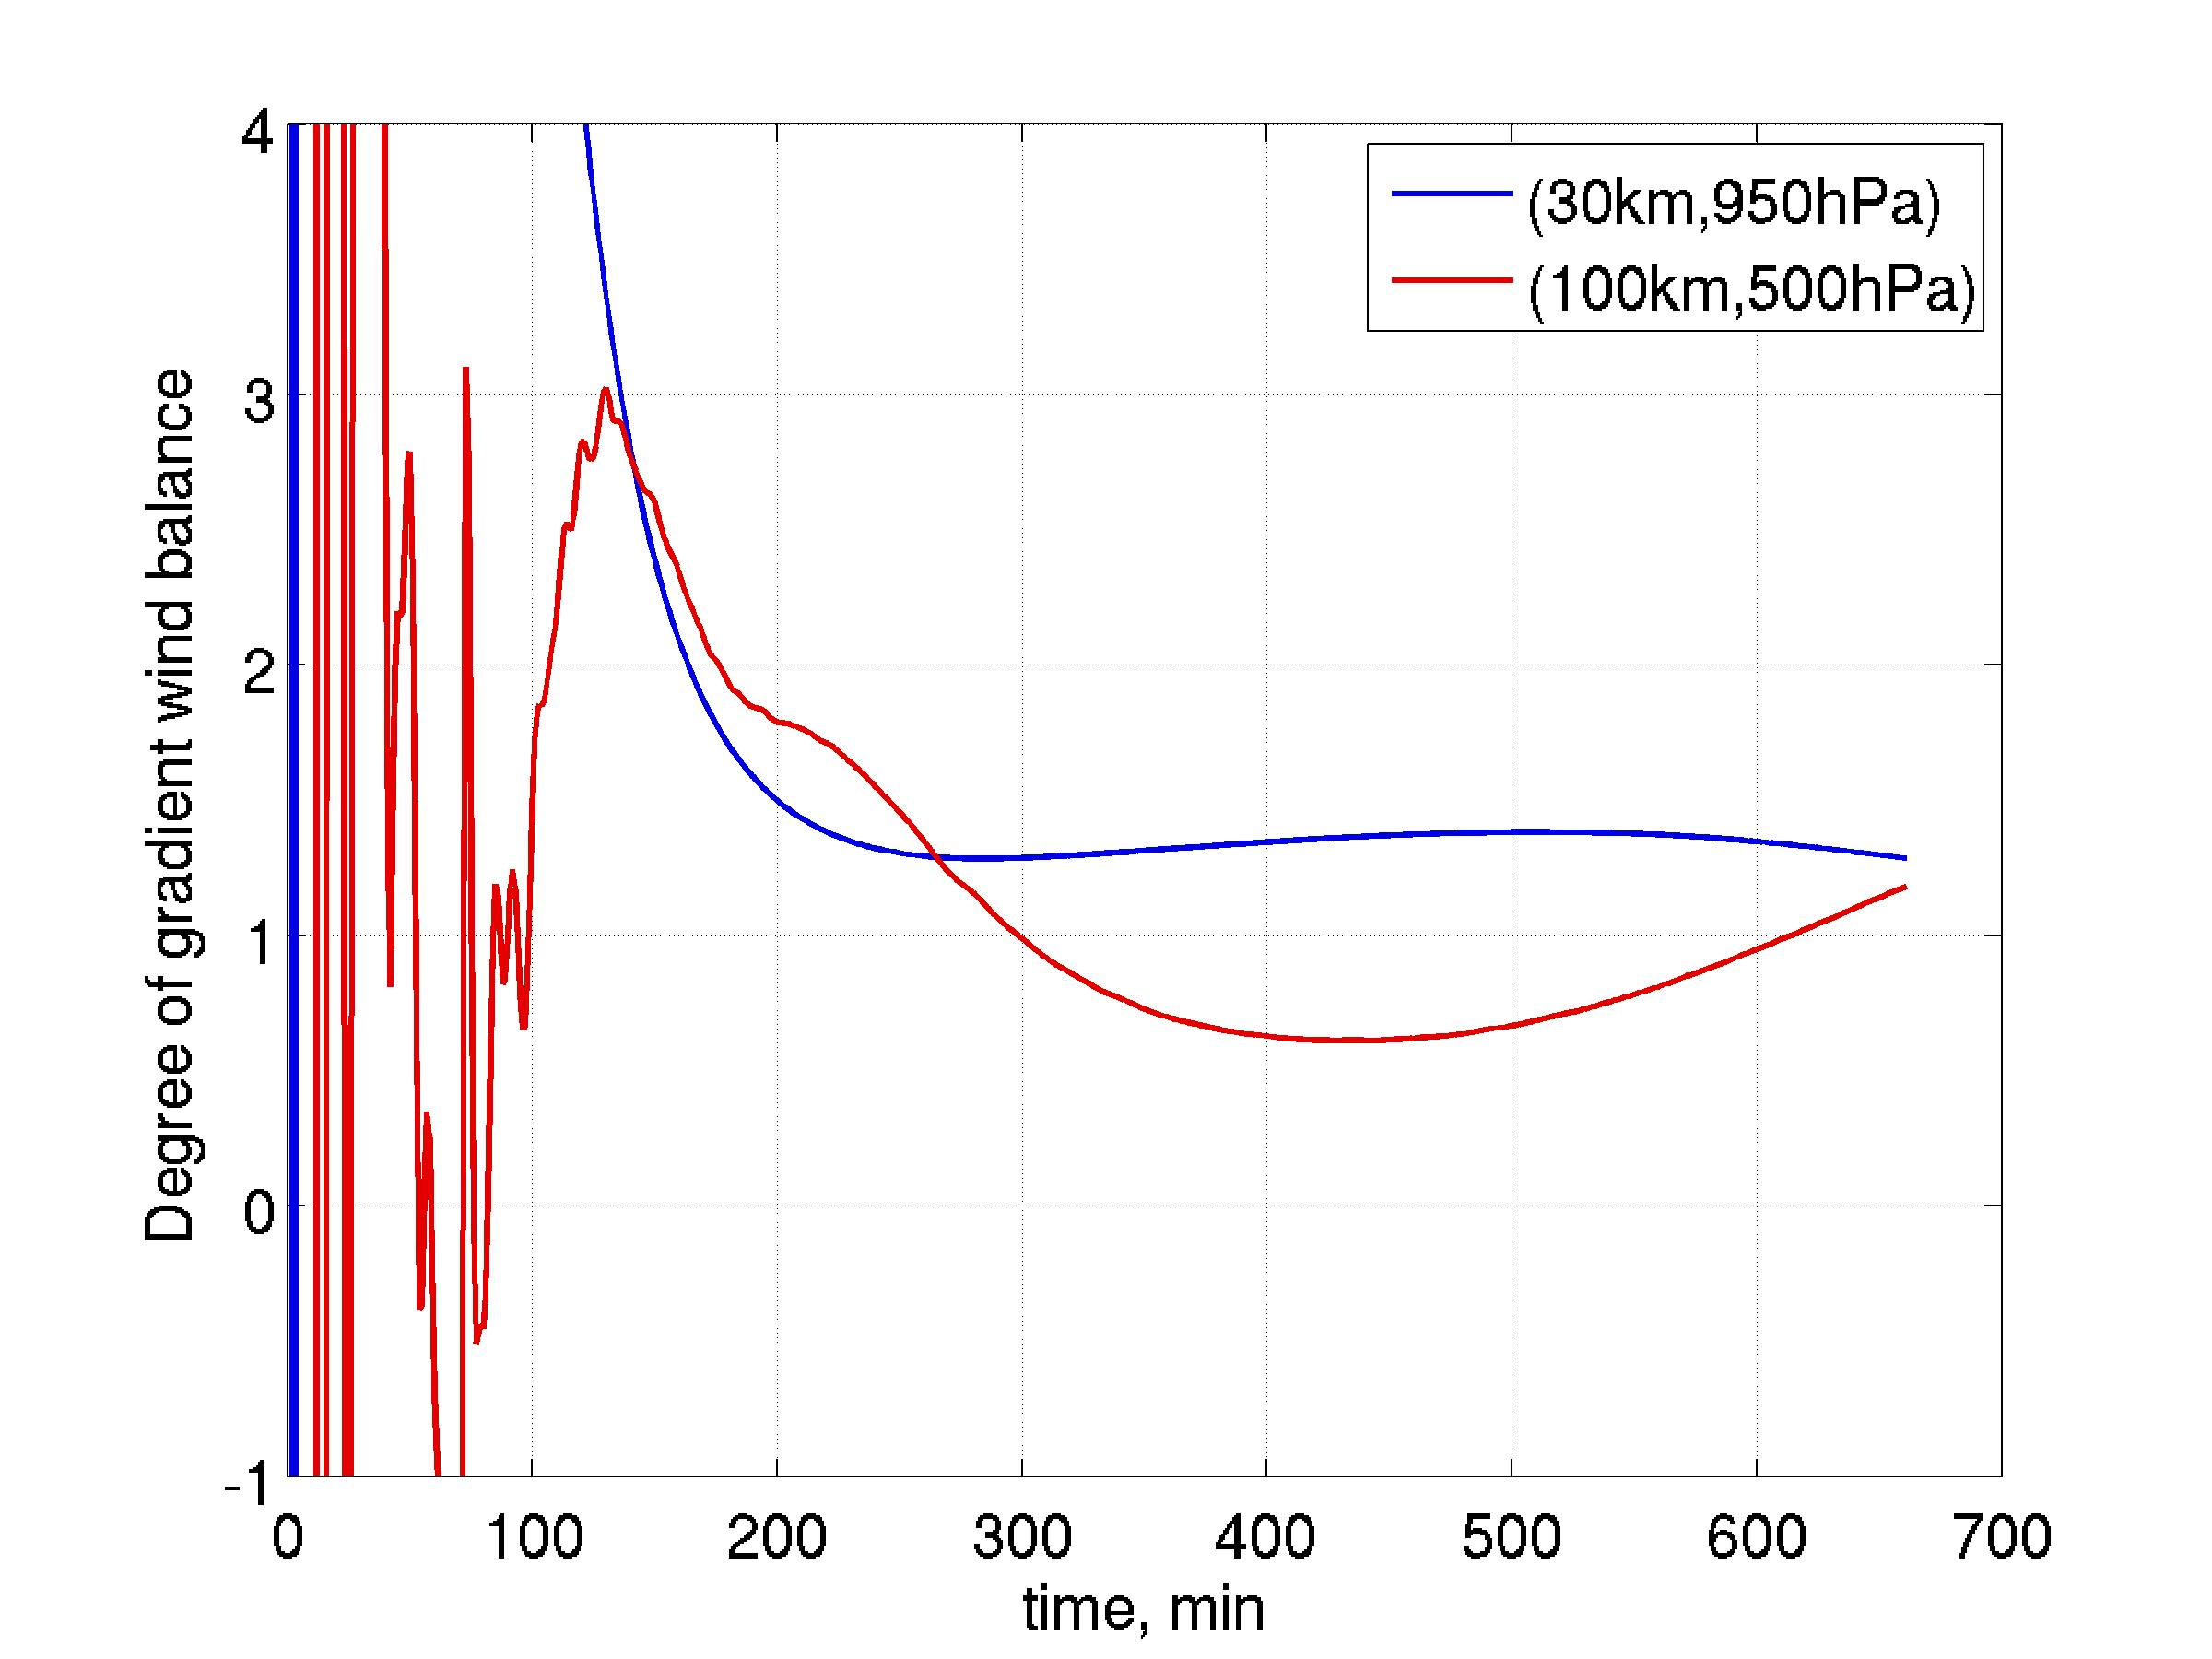
\includegraphics[width=\linewidth]{{./chapters/figures_results/ctrl_grwindbal2p}.jpg}
%\end{center}
%\caption{Вертикальный разрез вертикальной скорости $w$. Эксперимент CTRL. ??? час модельного времени.}
%\label{fig:ctrl_ene}
%\end{wrapfigure} 
%
%За счет чего развивается рассматриваемый мезоциклон? Для ответа на этот вопрос приводится бюджет кинетической энергии (рис. \ref{fig:ctrl_ene}), рассчитанный согласно ур. \ref{eq:dKdt}. Видно, что наиболее важными слагаемыми бюджета энергии являются слагаемое $C(A,K)$ перехода доступной потенциальной энергии в кинетическую и слагаемое диссипации кинетической энергии. Оба слагаемых растут по абсолютным значениям по мере роста энергии движения в вихре. 
%
%Интегральная величина $C(A,K)$ физически представляет собой поток силы плавучести $w\frac{\theta'}{\theta_s}$, суммированный по всей области. Его распределение в циклоне показано на рис. \ref{fig:ctrl_buoy_rz}. Можно заметить, что области экстремумов величины $w\frac{\theta'}{\theta_s}$ совпадают с областями наибольших и наименьших значений вертикальной скорости. Иными словами, конвертация ДПЭ в КЭ в моделируемом мезоциклоне наиболее интенсивна на радиусе максимальной скорости.
%Слагаемое $C(A,K)$, определяя тенденцию кинетической энергии, связывает ее с изменением доступной потенциальной энергии. При этом в бюджете последней это слагаемое имеет сравнительно малую долю (рис. \ref{}). Доступная потенциальная энергия в свою очередь генерируется за счет  слагаемого $H_{surf}$, связанного с потоками тепла на нижней границе области (\ref{sec:expsetup:hsurf}).
%
%\section{'Влажный' эксперимент: эффекты конденсации} 
%
%\begin{wrapfigure}{R}{0.5\textwidth}
%\begin{center}
%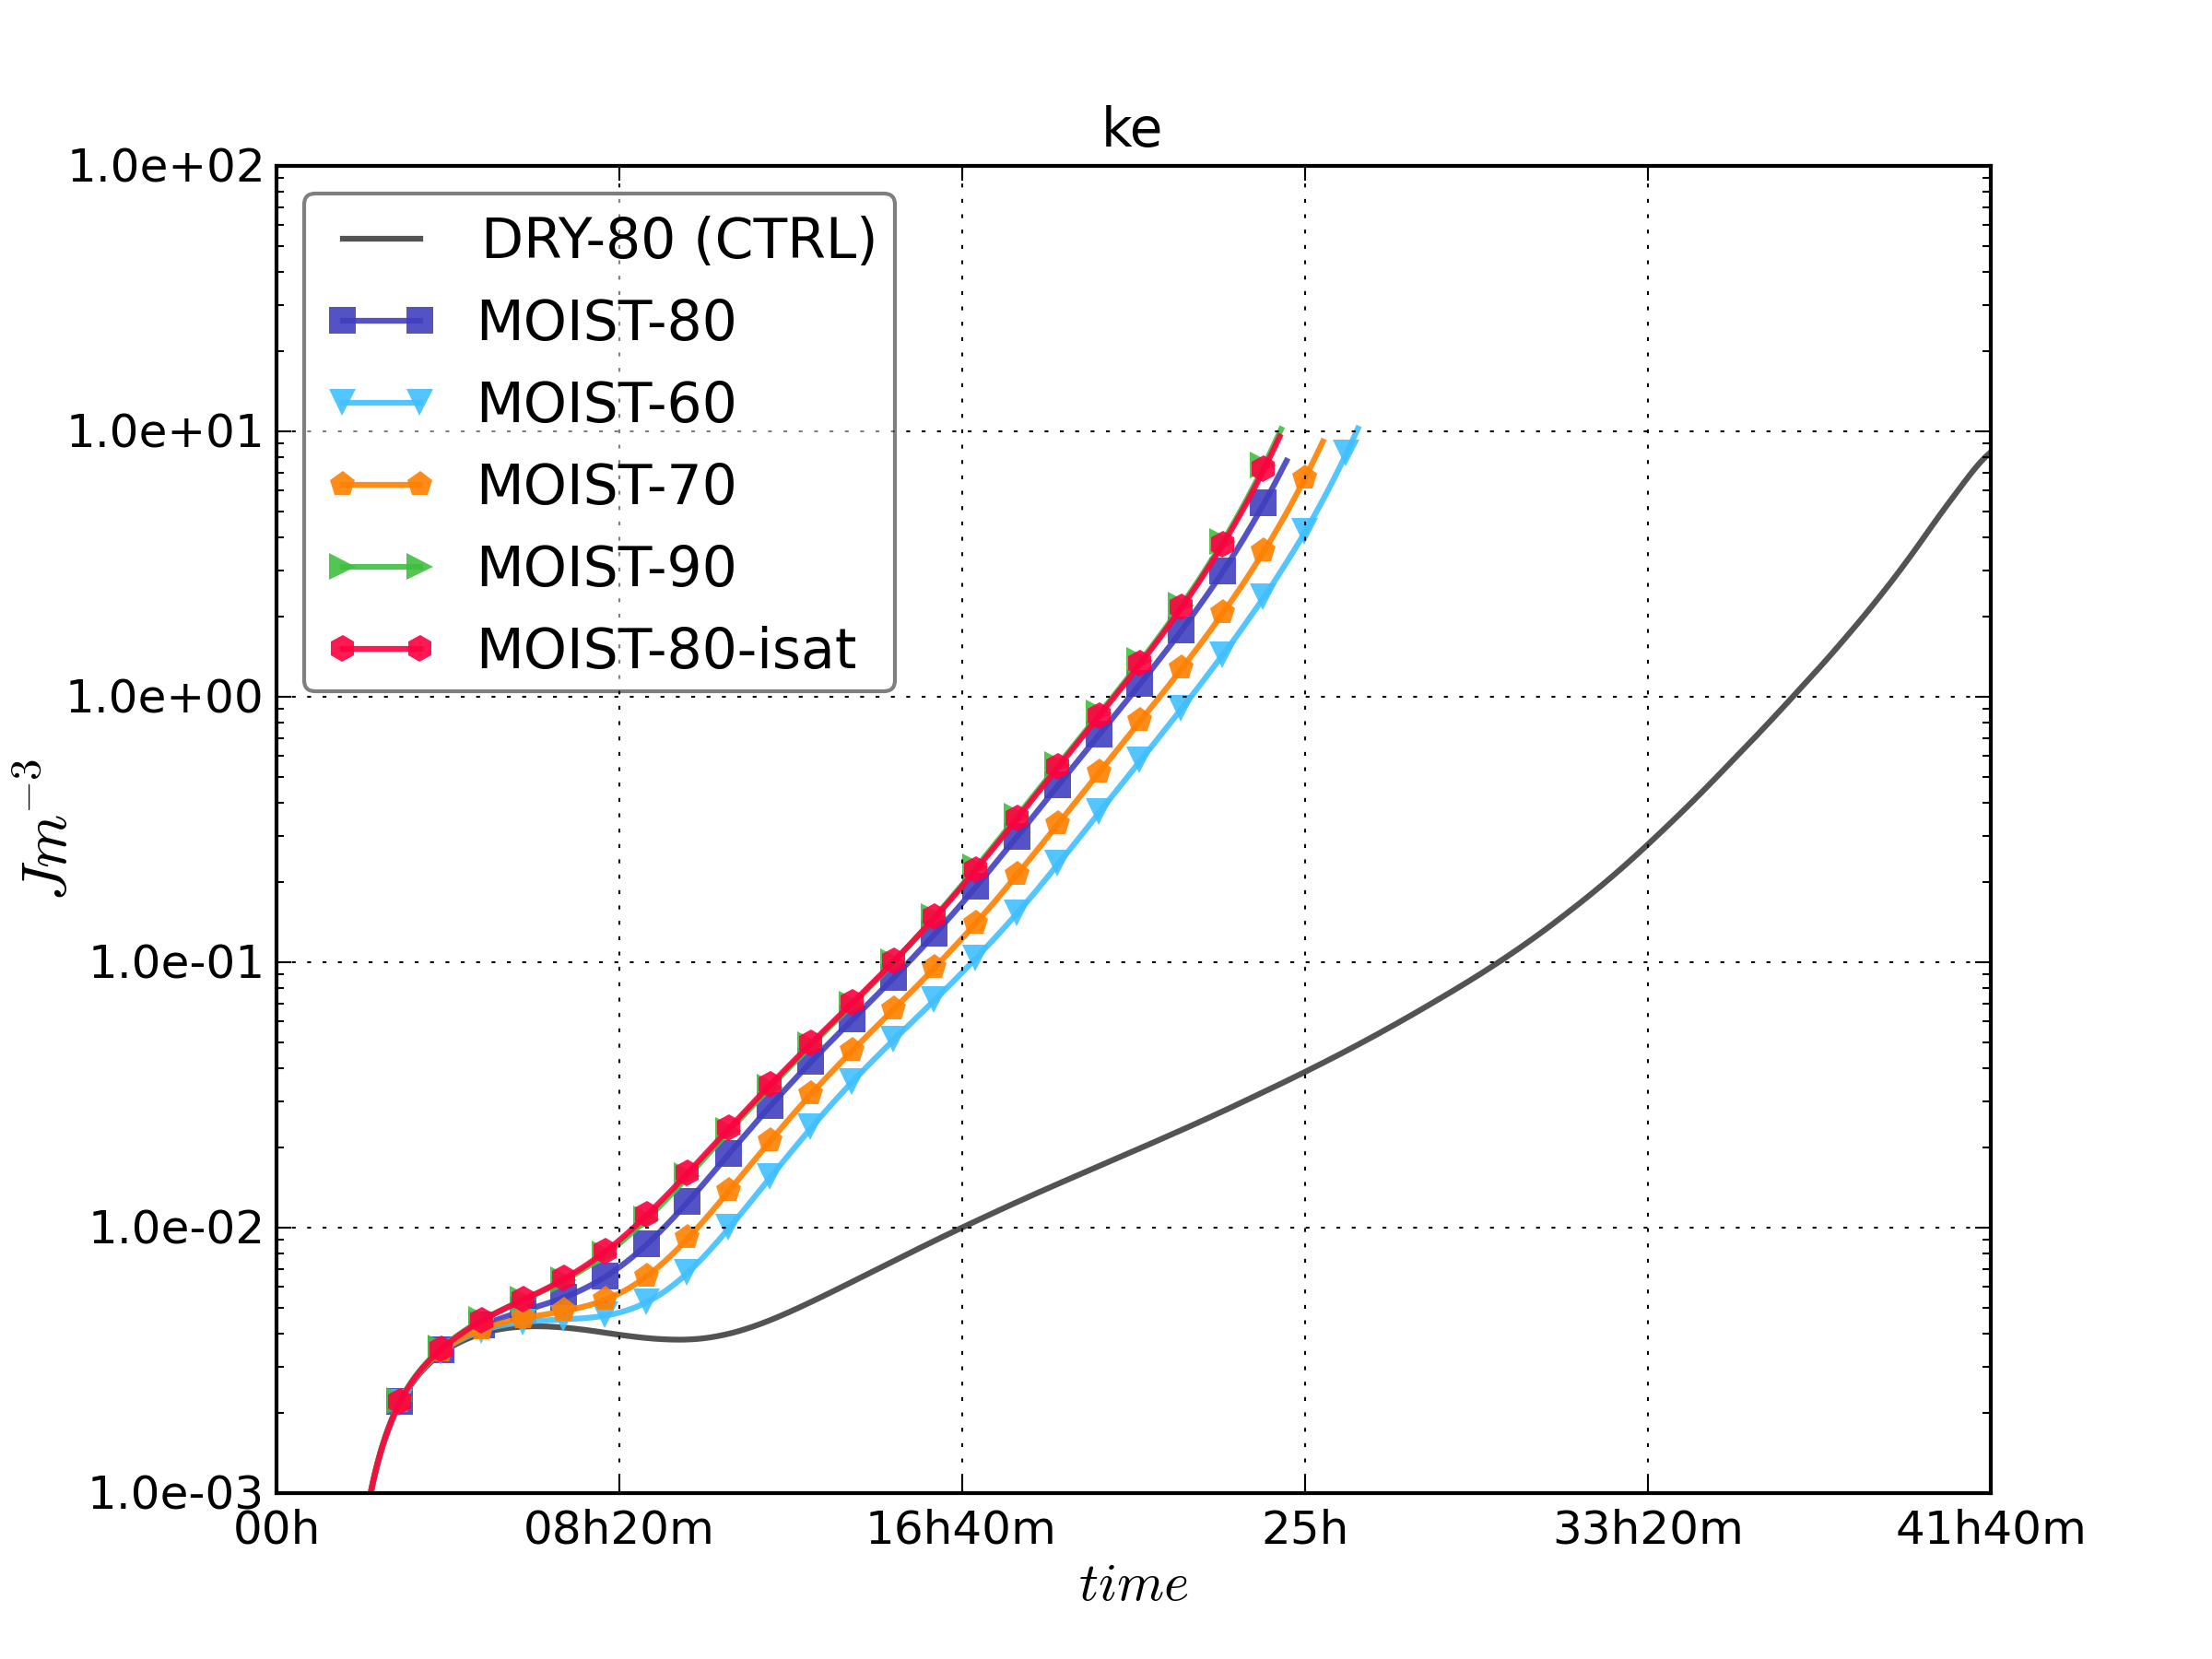
\includegraphics[width=\linewidth]{{./chapters/figures_results/ke.00h-41h38m.DRYvsMOIST}.png}
%\end{center}
%\caption{Эволюция кинетической энергии в экспериментах MOIST по сравнению с контрольным (здесь и далее черная кривая).}
%\label{fig:moist_ke}
%\end{wrapfigure} 
%
%Напомним, что описанный выше контрольный эксперимент является 'сухим': процессы конденсации были отключены, несмотря на то, что относительная влажность в центре области довольно скоро начала превышать $100\%$. Для того, чтобы оценить влияние конденсации в атмосфере как дополнительного источника тепла, проанализируем серию 'влажных' экспериментов (MOIST). На рис. \ref{fig:moist_ke} представлено изменение кинетической энергии со временем экспериментах MOIST (цветные кривые) по сравнению с контрольным экспериментом (DRY, черная кривая). Эксперименты с конденсацией характеризуются большей скоростью роста энергии и, соответственно, меньшим временем устойчивости эксперимента: вихрь развивается до предельных скоростей ветра ровно за сутки. 
%
%Аналогичное соотношение между сухим и влажным экспериментом дает сравнение роста аномалии приземного давления ($SLP_{anom}$), который показан на рис. \ref{fig:moist_slp}. Максимальное падение давления в центре в эксперименте MOIST-80 составляет $-32.6\hpa$, в то время как в контрольном эксперименте (черная кривая) минимум давления в центре вихря достигает $19.8\hpa$.
%
%\begin{wrapfigure}{L}{0.5\textwidth}
%\begin{center}
%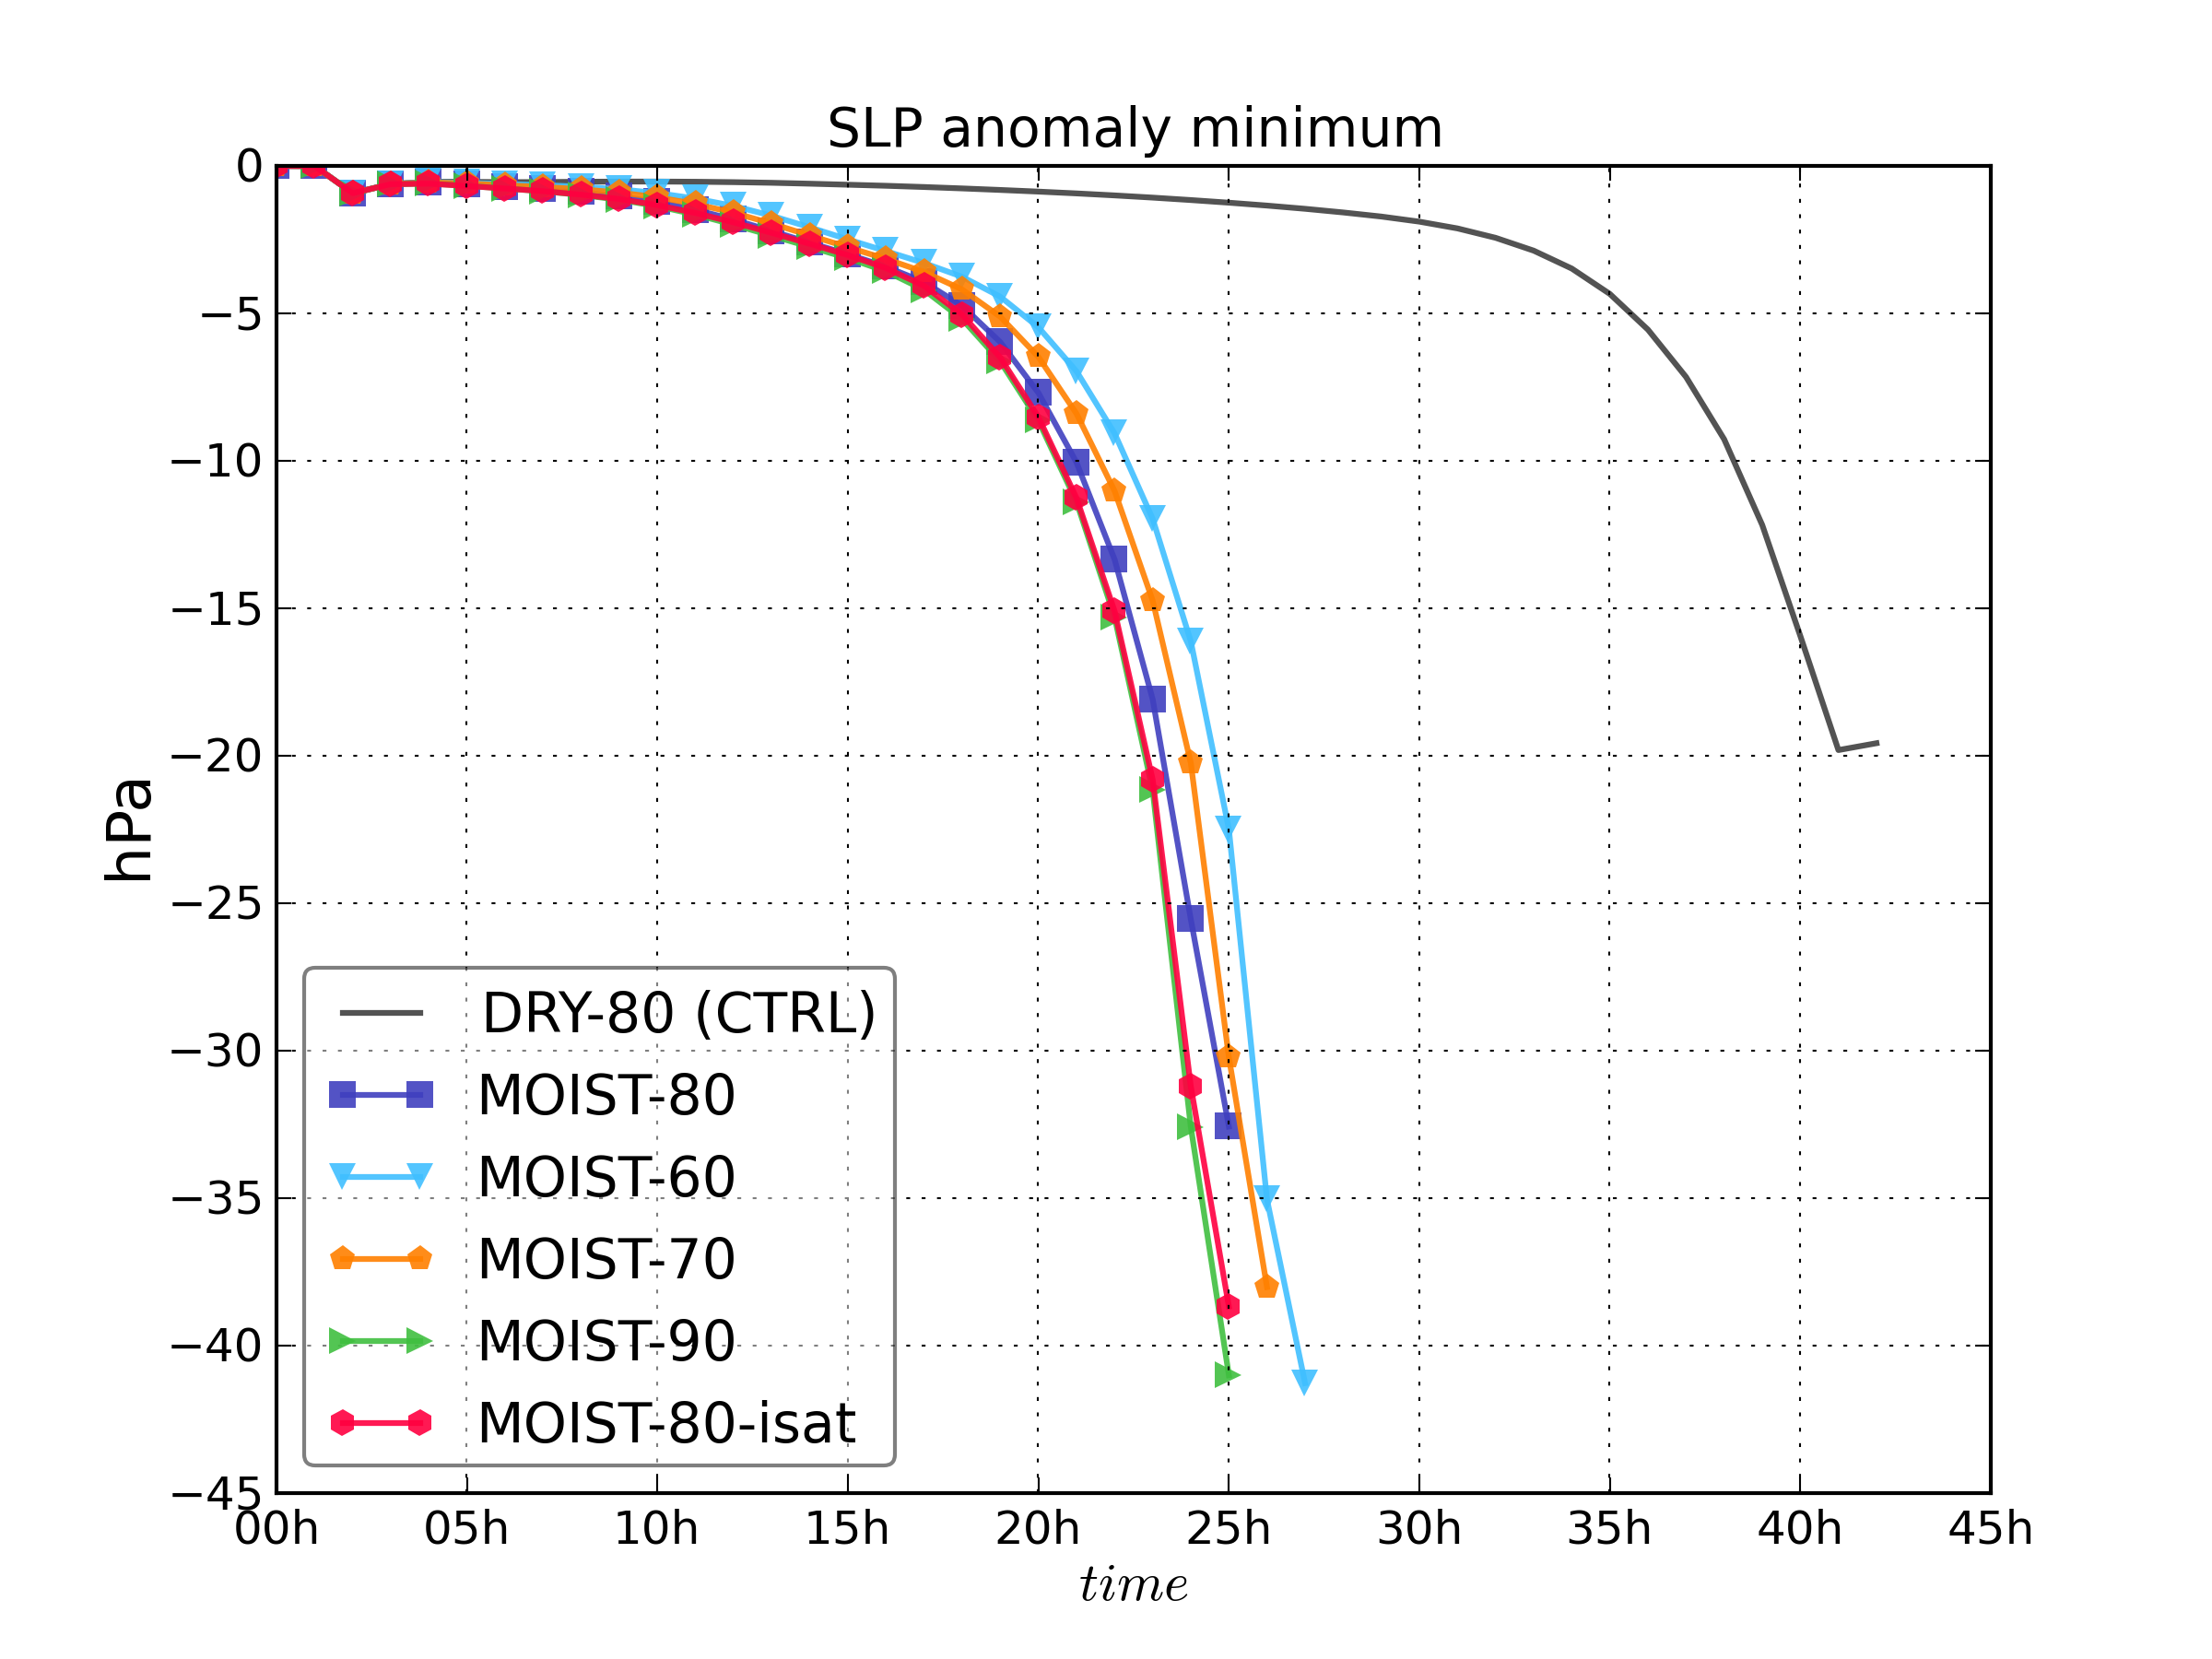
\includegraphics[width=\linewidth]{{./chapters/figures_results/slp_min.00h-42h.DRYvsMOIST}.png}
%\end{center}
%\caption{Эволюция аномалии приземного давления в экспериментах MOIST по сравнению с контрольным.}
%\label{fig:moist_slp}
%\end{wrapfigure} 
%
%Представленные графики показывают зависимость интенсивности вихря от начального содержания влаги в атмосфере: чем больше относительная влажность воздуха задана в начальный момент, тем интенсивнее происходит развитие вихря: так, в  25 час модельного времени аномалия приземного давления составляет от $-22\hpa$ до $-41\hpa$ для экспериментов от MOIST-60 до MOIST-90 соответственно.
%
%Проведенные эксперименты позволяют оценить чувствительность динамики вихря к содержанию влаги в атмосфере. Сначала определим показатель интенсивности вихря как единый количественный критерий для всех экспериментов, разделив минимум аномалии приземного давления в расчетной области на время достижения этого минимума. Это позволит более корректно сравнивать эксперименты, в которых циклон развивался до одинаковой силы, но за разный период времени. Иначе говоря, в качестве показателя интенсивности вихря берется средняя барическая тенденция:
%\begin{equation} \label{eq:intensity}
%I = \frac{SLP_{anom}}{\tau},
%\end{equation}
%где $SLP_{anom}$ --- аномалия приземного давления (\ref{eq:slpanom}), $\tau$ --- продолжительность экспепримента ($\tau_{max}=72$ ч.). Разность между интенсивностью вихря $I$ в контрольном эксперименте и интенсивностью в оценочном эксперименте, отнесенная к разности значения какого-либо параметра $P$ (в данном случае начальной влажности воздуха) дает показатель чувствительности:
%\begin{equation}
%S_{slp}=\frac{\delta I}{\delta P}.
%\end{equation}
%Используя этот показатель, результаты серии оценочных экспериментов MOIST можно представить в количественном выражении (табл. \ref{}, аналогично \citep{LindersEtAl2011}).
%
%\begin{table}
%\end{table}
%
%Кривая MOIST-80-isat относится к эксперименту, в котором фазовые переходы воды зависят от формулы давления насыщения водяного пара надо льдом, а относительная влажность воздуха равна контрольной. На рис. \ref{fig:moist_ke} и \ref{fig:moist_slp} эта кривая почти совпадает с кривой MOIST-90, т.е. использование в модели формулы Магнуса (закона Клаузиуса-Клапейрона) для давления насыщения водяного пара надо льдом по сравнению с таковой для давления насыщения над водой равносильно ошибке в задании начальной относительной влажности, равной около $10\%$. Однако к кардинальным отличиям в динамике вихря использование той или иной формулы не ведет.
%
%\subsection{Энергетическая диагностика}
%Различия в темпах роста мезоциклона в рассматриваемых экспериментах можно рассмотреть с точки зрения генерации кинетической энергии. Как и в контрольном эксперименте, основной вклад в бюджет кинетической энергии вносит слагаемое $C(A,K)$, которое по значениям также пропорционально количеству влаги в атмосфере. На рис. \ref{fig:moist_dkdt}, где представлены компоненты энергии для выбранных случаев, четко прослеживается отличие контрольного эксперимента от серии MOIST, причем это наблюдается для всех величин ввиду их нелинейности.
%
%\begin{wrapfigure}{R}{0.5\textwidth}
%\begin{center}
%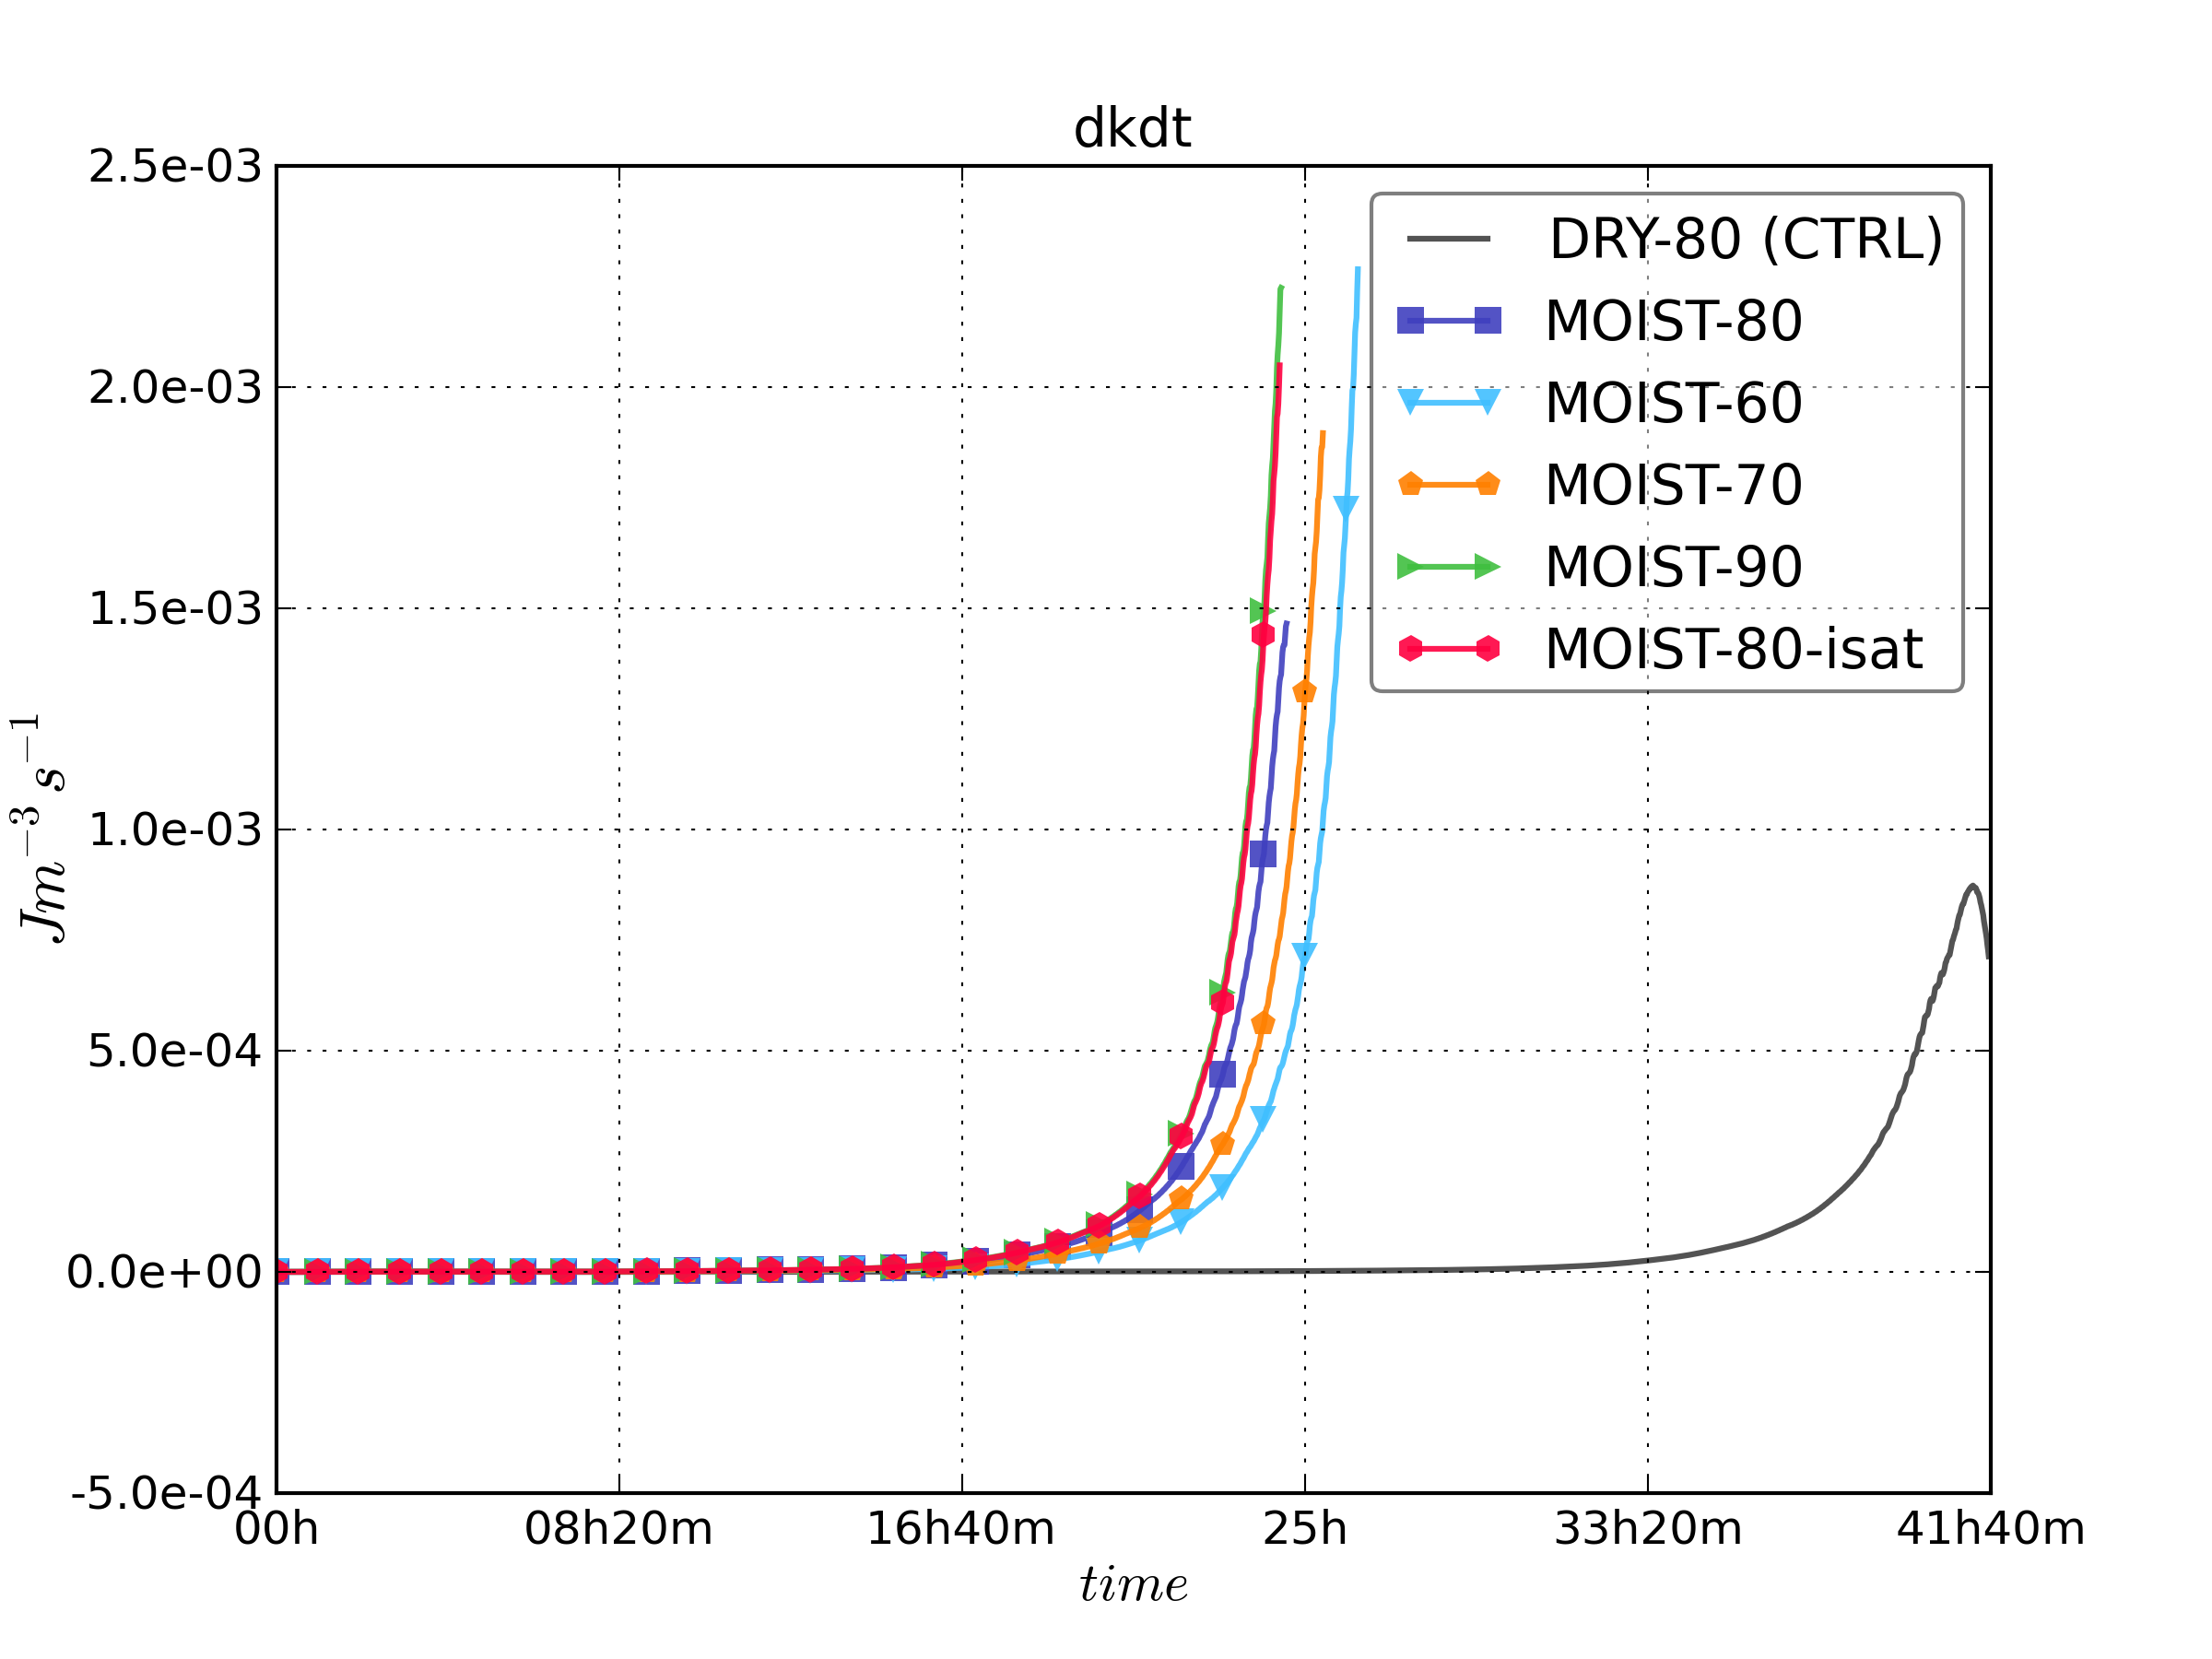
\includegraphics[width=\linewidth]{{./chapters/figures_results/dkdt.00h-41h38m.DRYvsMOIST}.png}
%\end{center}
%\caption{Изменение скорости роста кинетической энергии в экспериментах MOIST по сравнению с контрольным.}
%\label{fig:moist_dkdt}
%\end{wrapfigure} 
%
%Дополнительным источником энергии для роста циклона, очевидно, являются неадиабатические процессы, т.е. выделение скрытого тепла конденсации (ур. \ref{eq:progn4}, второе слагаемое в правой части). В ходе анализа экспериментов недиабатический приток тепла был рассчитан по остаточному методу \citep{Muench1965,MooreMontgomery2005}:
%\begin{equation}
%Q=\left[\pderiv{\theta}{t}+\vec{v}\cdot\nabla_h\theta+\omega\pderiv{\theta}{p}\right]c_p\left(\frac{p}{p_{00}}\right)^{R_d/c_p},
%\end{equation}
%где $\pderiv{}{t}+\vec{v}\cdot\nabla_h+\omega\pderiv{}{p}$ --- полная производная в $p$-системе координат. Расчет проводился по данным, интерполированным на изобарические поверхности. Далее для удобства величину $Q$ разделим на $c_p$ и умножим на $86400$, получив размерность $\K~\text{день}^{-1}$. На рис. \ref{} представлено сравнение недиабатического притока тепла для выбранных экспериментов, из которого понятно, что в каждом эксперименте рост этой величины начинается в разное время для разных экспериментов, так как состояние насыщения достигается тем быстрее, чем больше относительное влагосодержание воздуха при инициализации. Для контрольного эксперимента же недиабатический приток тепла остается на уровне ??? $\K~\text{день}^{-1}$ (вклад потоков тепла с поверхности).
%
%\subsection{Структура и эволюция вихря}
%Вклад энергии от фазовых переходов воды отражается на строении моделируемого мезоциклона. Для этого на рис. \ref{} приведены радиальные разрезы основных метеорологических полей, полученные в эксперименте MOIST-80, за 18 час модельного времени, когда скорость ветра в мезоциклоне сопоставима с таковой  в контрольном эксперименте за 36 час.
%
%В основном, различие между контрольным экспериментом (DRY-80) и MOIST-80 проявляется в распределении влагосодержания воздуха: вблизи центра вихря закономерно происходит уменьшение содержания водяного пара в процессе конденсации. Распределение конденсации в циклоне находится в соответствии с полем относительной влажности (рис. \ref{}), и максимум приходится на область конвективных движений (рис. \ref{}) на расстоянии $30$--$40\km$ от центра и на высоте $2000\m$. Из представленных разрезов также ясно, что слабая конденсация происходит и на периферии вихря вследствие турбулентного потока влаги с поверхности.
%
%\section{Серия с разной устойчивостью атмосферы}
%\subsection{Влияние устойчивости атмосферы на интенсивность вихря}
%К важным факторам, оказывающим влияние на развитие атмосферных неоднородностей, относится стратификация атмосферы. Размеры возмущений и статификацию объединяет в себе радиус деформации Россби ($R=\frac{Nf}{L}$). Это число показывает, что вертикальный масштаб циклона, возникшего в результате нагрева, обратно пропорционально статической устойчивости и прямо пропорционально абсолютной завихренности и горизонтальному масштабу объекта.
%
%\begin{figure}[h]
%	\centering
%	\begin{subfigure}{0.45\textwidth}
%		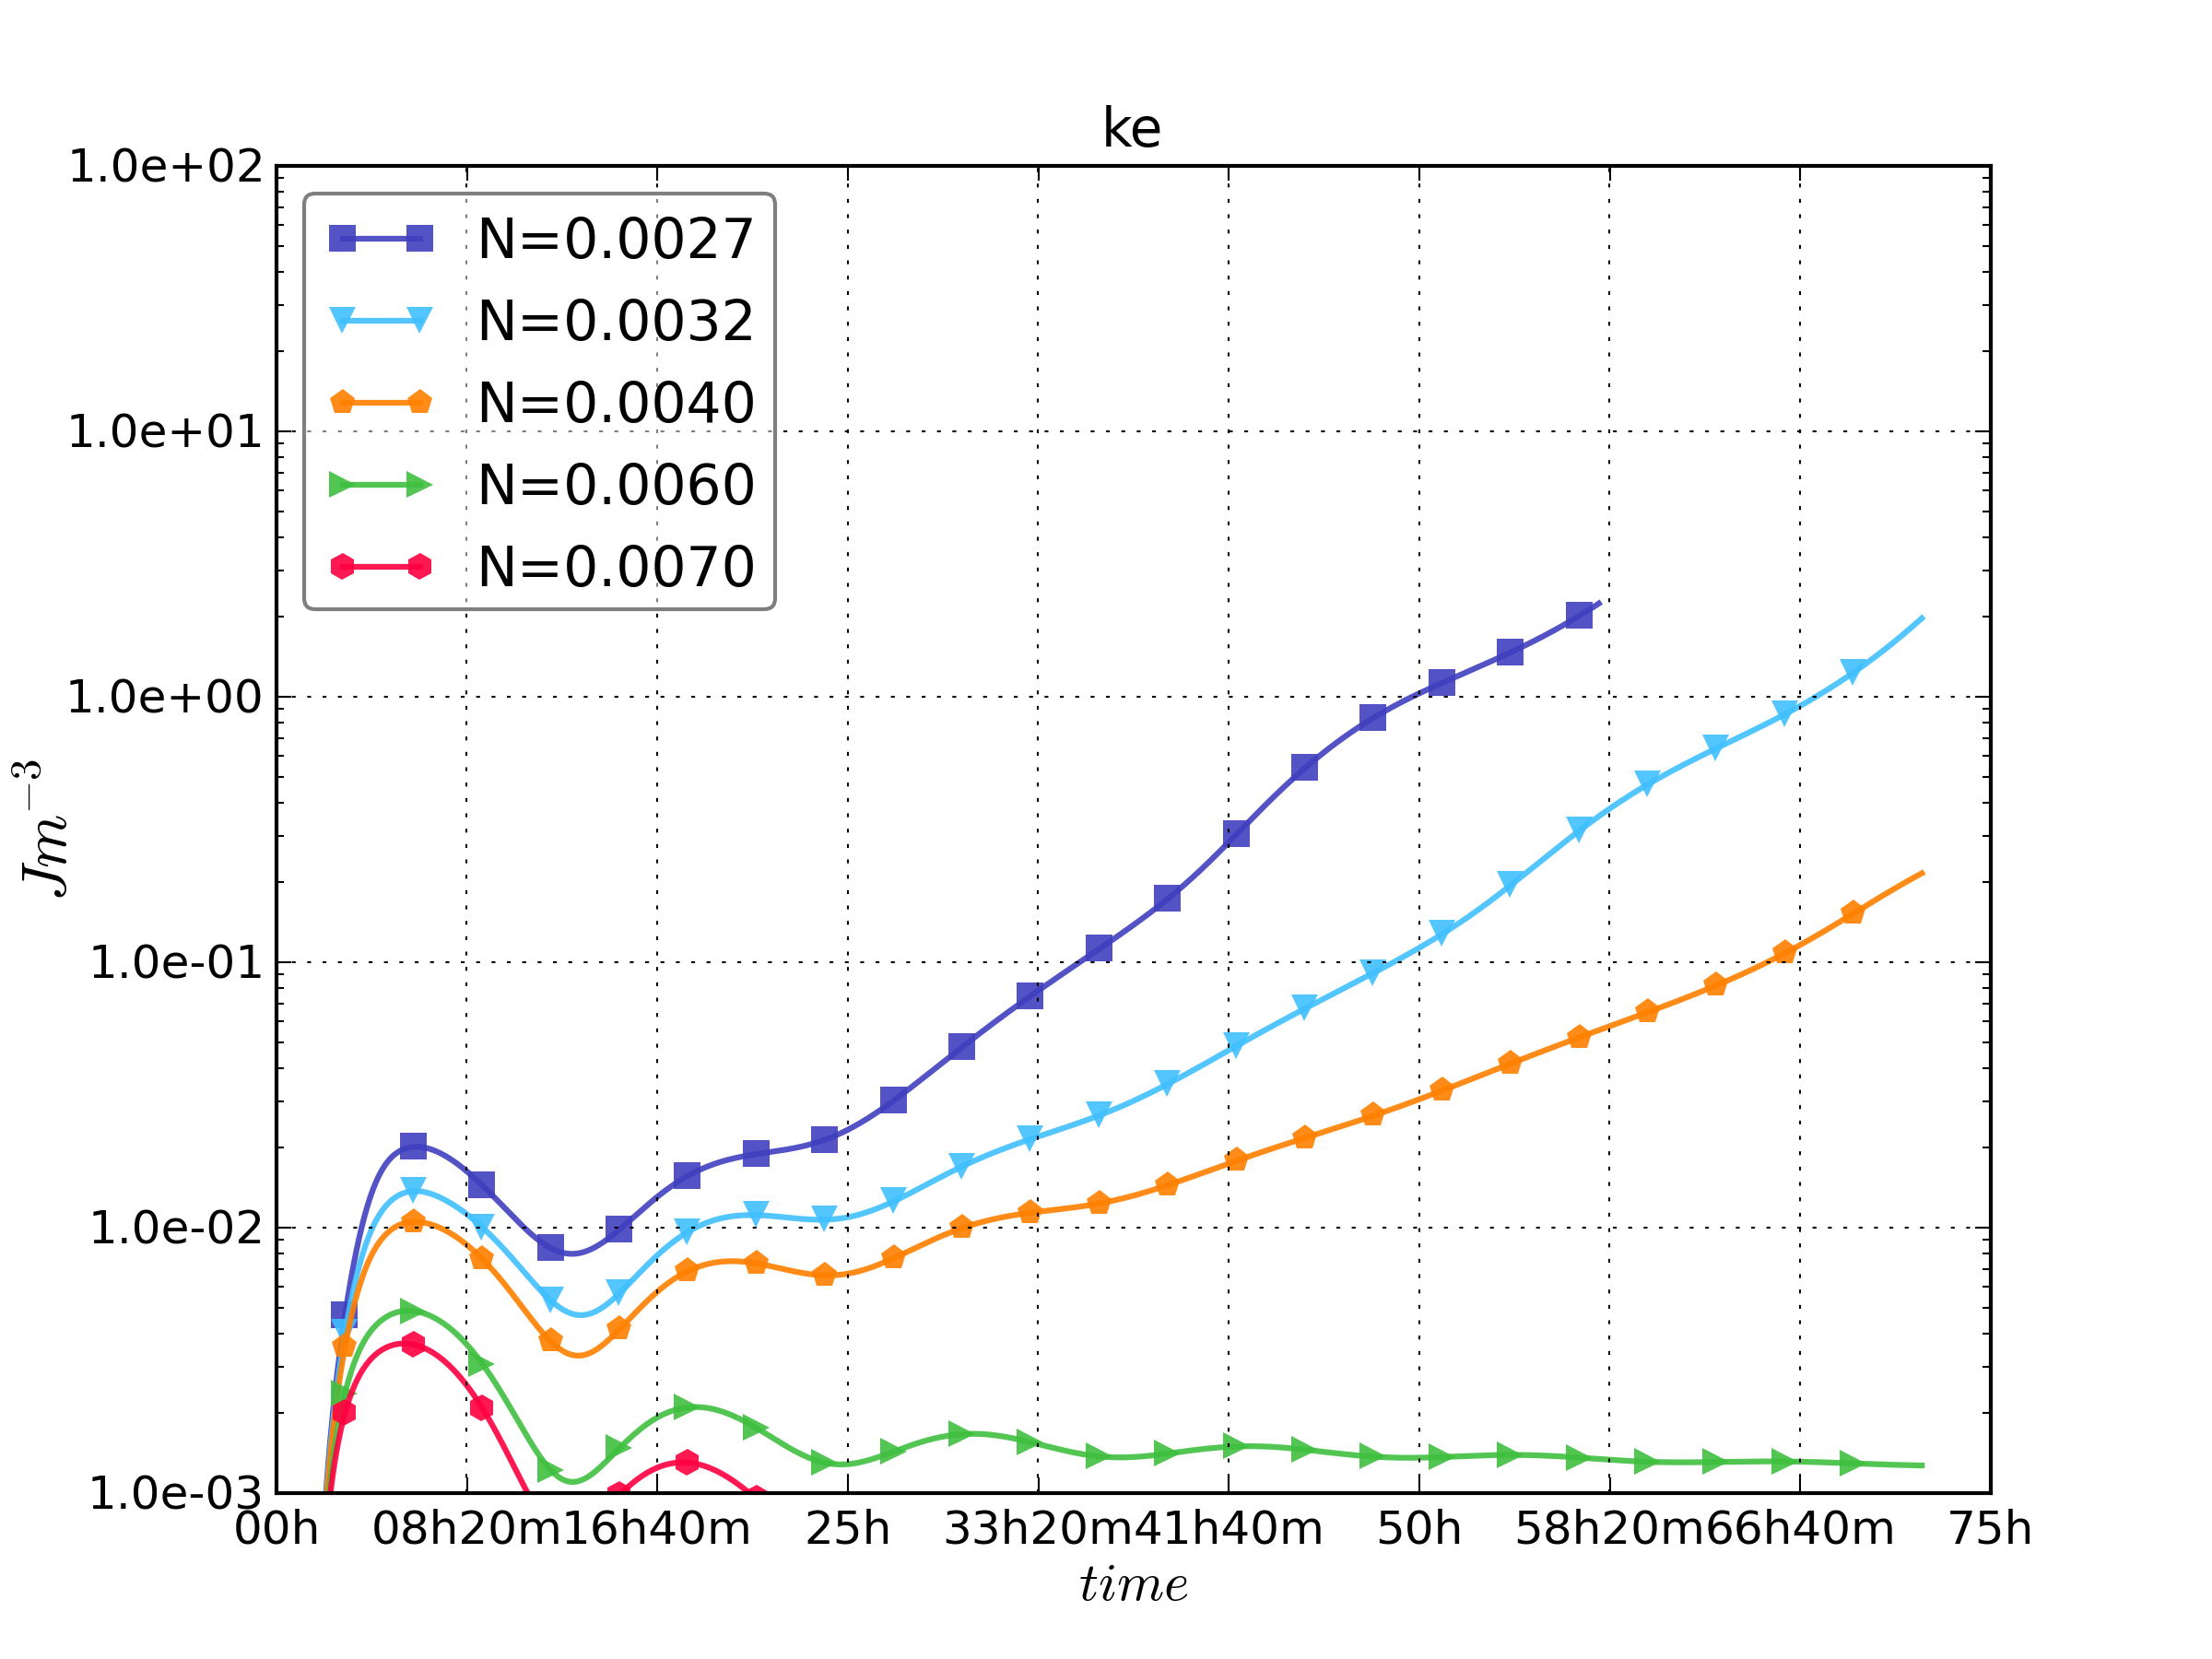
\includegraphics[width=\linewidth]{{./chapters/figures_results/ke.00h-72h.lowN}.png}
%		\caption{ }
%        \label{fig:lowN_ke}
%	\end{subfigure}
%	\hfill
%	\begin{subfigure}{0.45\textwidth}
%		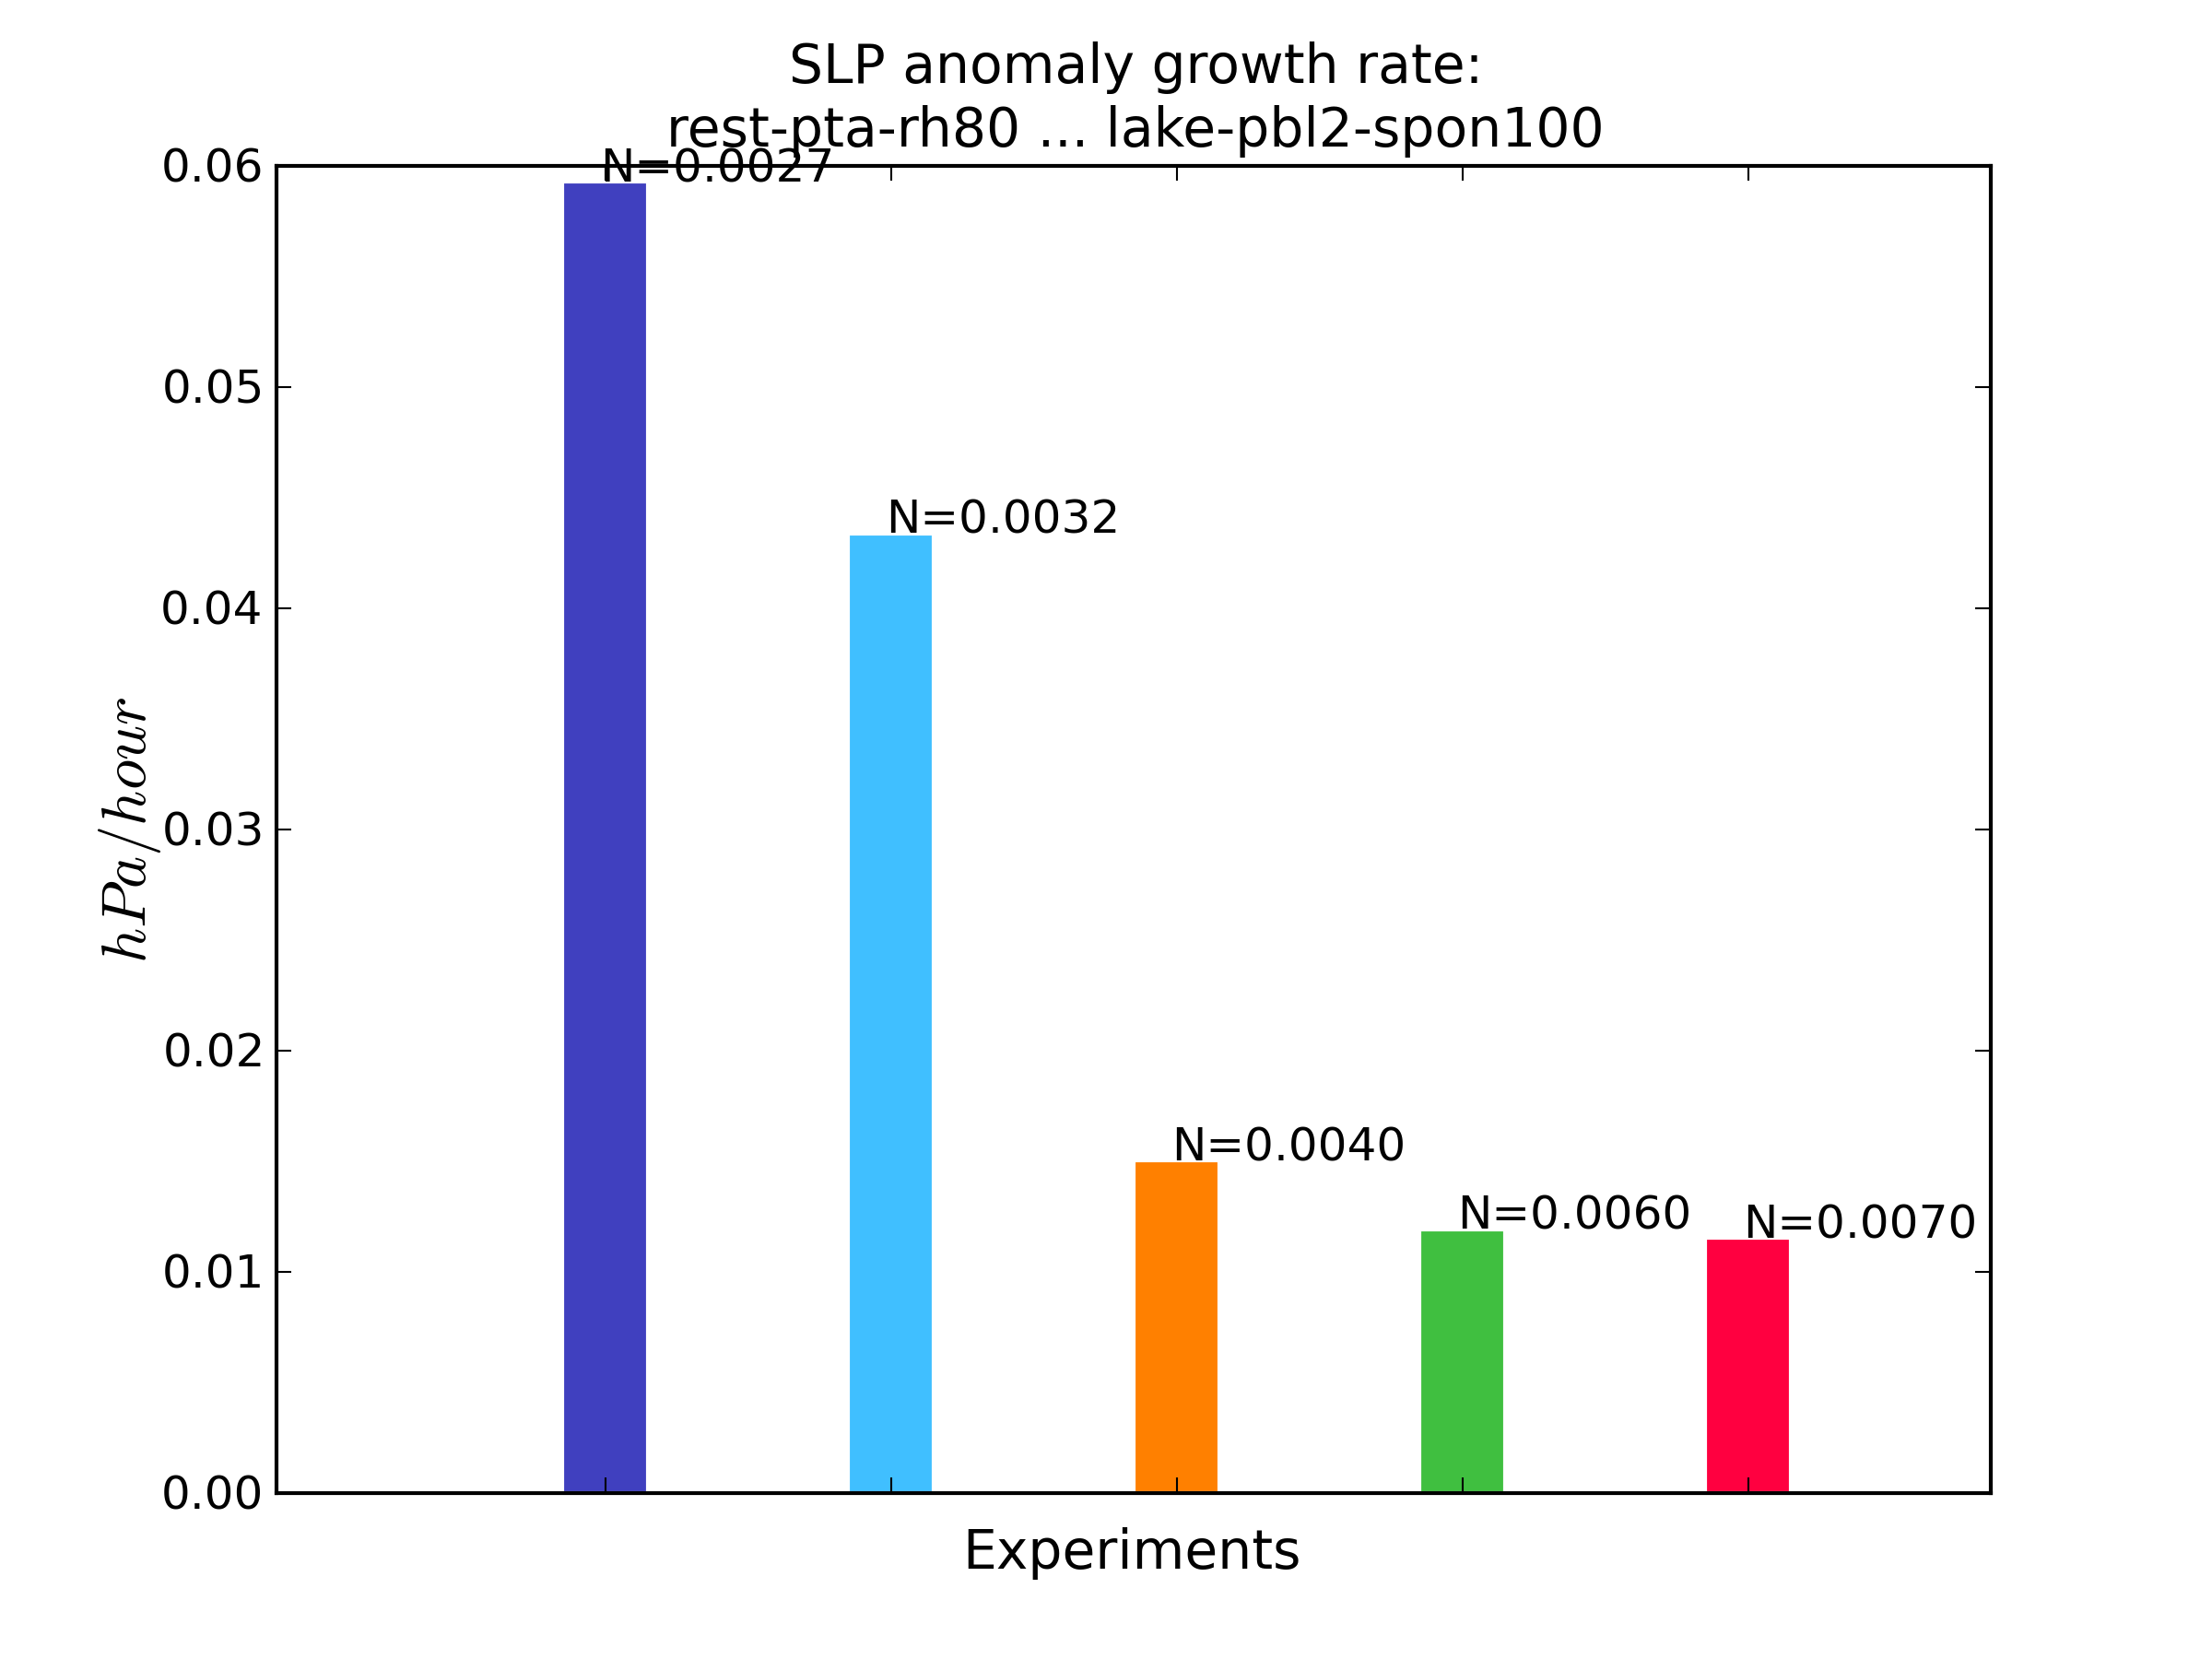
\includegraphics[width=\linewidth]{{./chapters/figures_results/slp_min_rate.00h-73h.lowN}.png}
%		\caption{ }
%		\label{fig:lowN_slp_rate}
%	\end{subfigure}
%        \caption{Эксперименты с пониженной устойчивостью фоновой атмосферы: изменение во времени кинетической энергии (слева) и чувствительность вихря к $N$ (справа).}
%\end{figure}
%
%Чувствительность развивающегося мезоциклона к устойчивости атмосферы была оценена с помощью серии экспериментов, в которых при неизменной температуре нижнего слоя менялась температура остальной толщи атмосферы, создавая вертикальный градиент потенциальной температуры от $0.2\Kpkm$ до $8\Kpkm$. То есть диапазон условий варьировался от статически нейтральной стратификации до устойчивой стратификации, характерной для арктических воздушных масс и в среднем наблюдающейся при генерации мезоциклонов \citep{ForbesLottes1985}. Частота Брента-Вяйсяля $N$ как показатель устойчивости атмосферы имел для фоновой стратификации значения $0.0027$--$0.0160\pers$ соответственно.
%
%\begin{figure}[h]
%	\centering
%	\begin{subfigure}{0.45\textwidth}
%		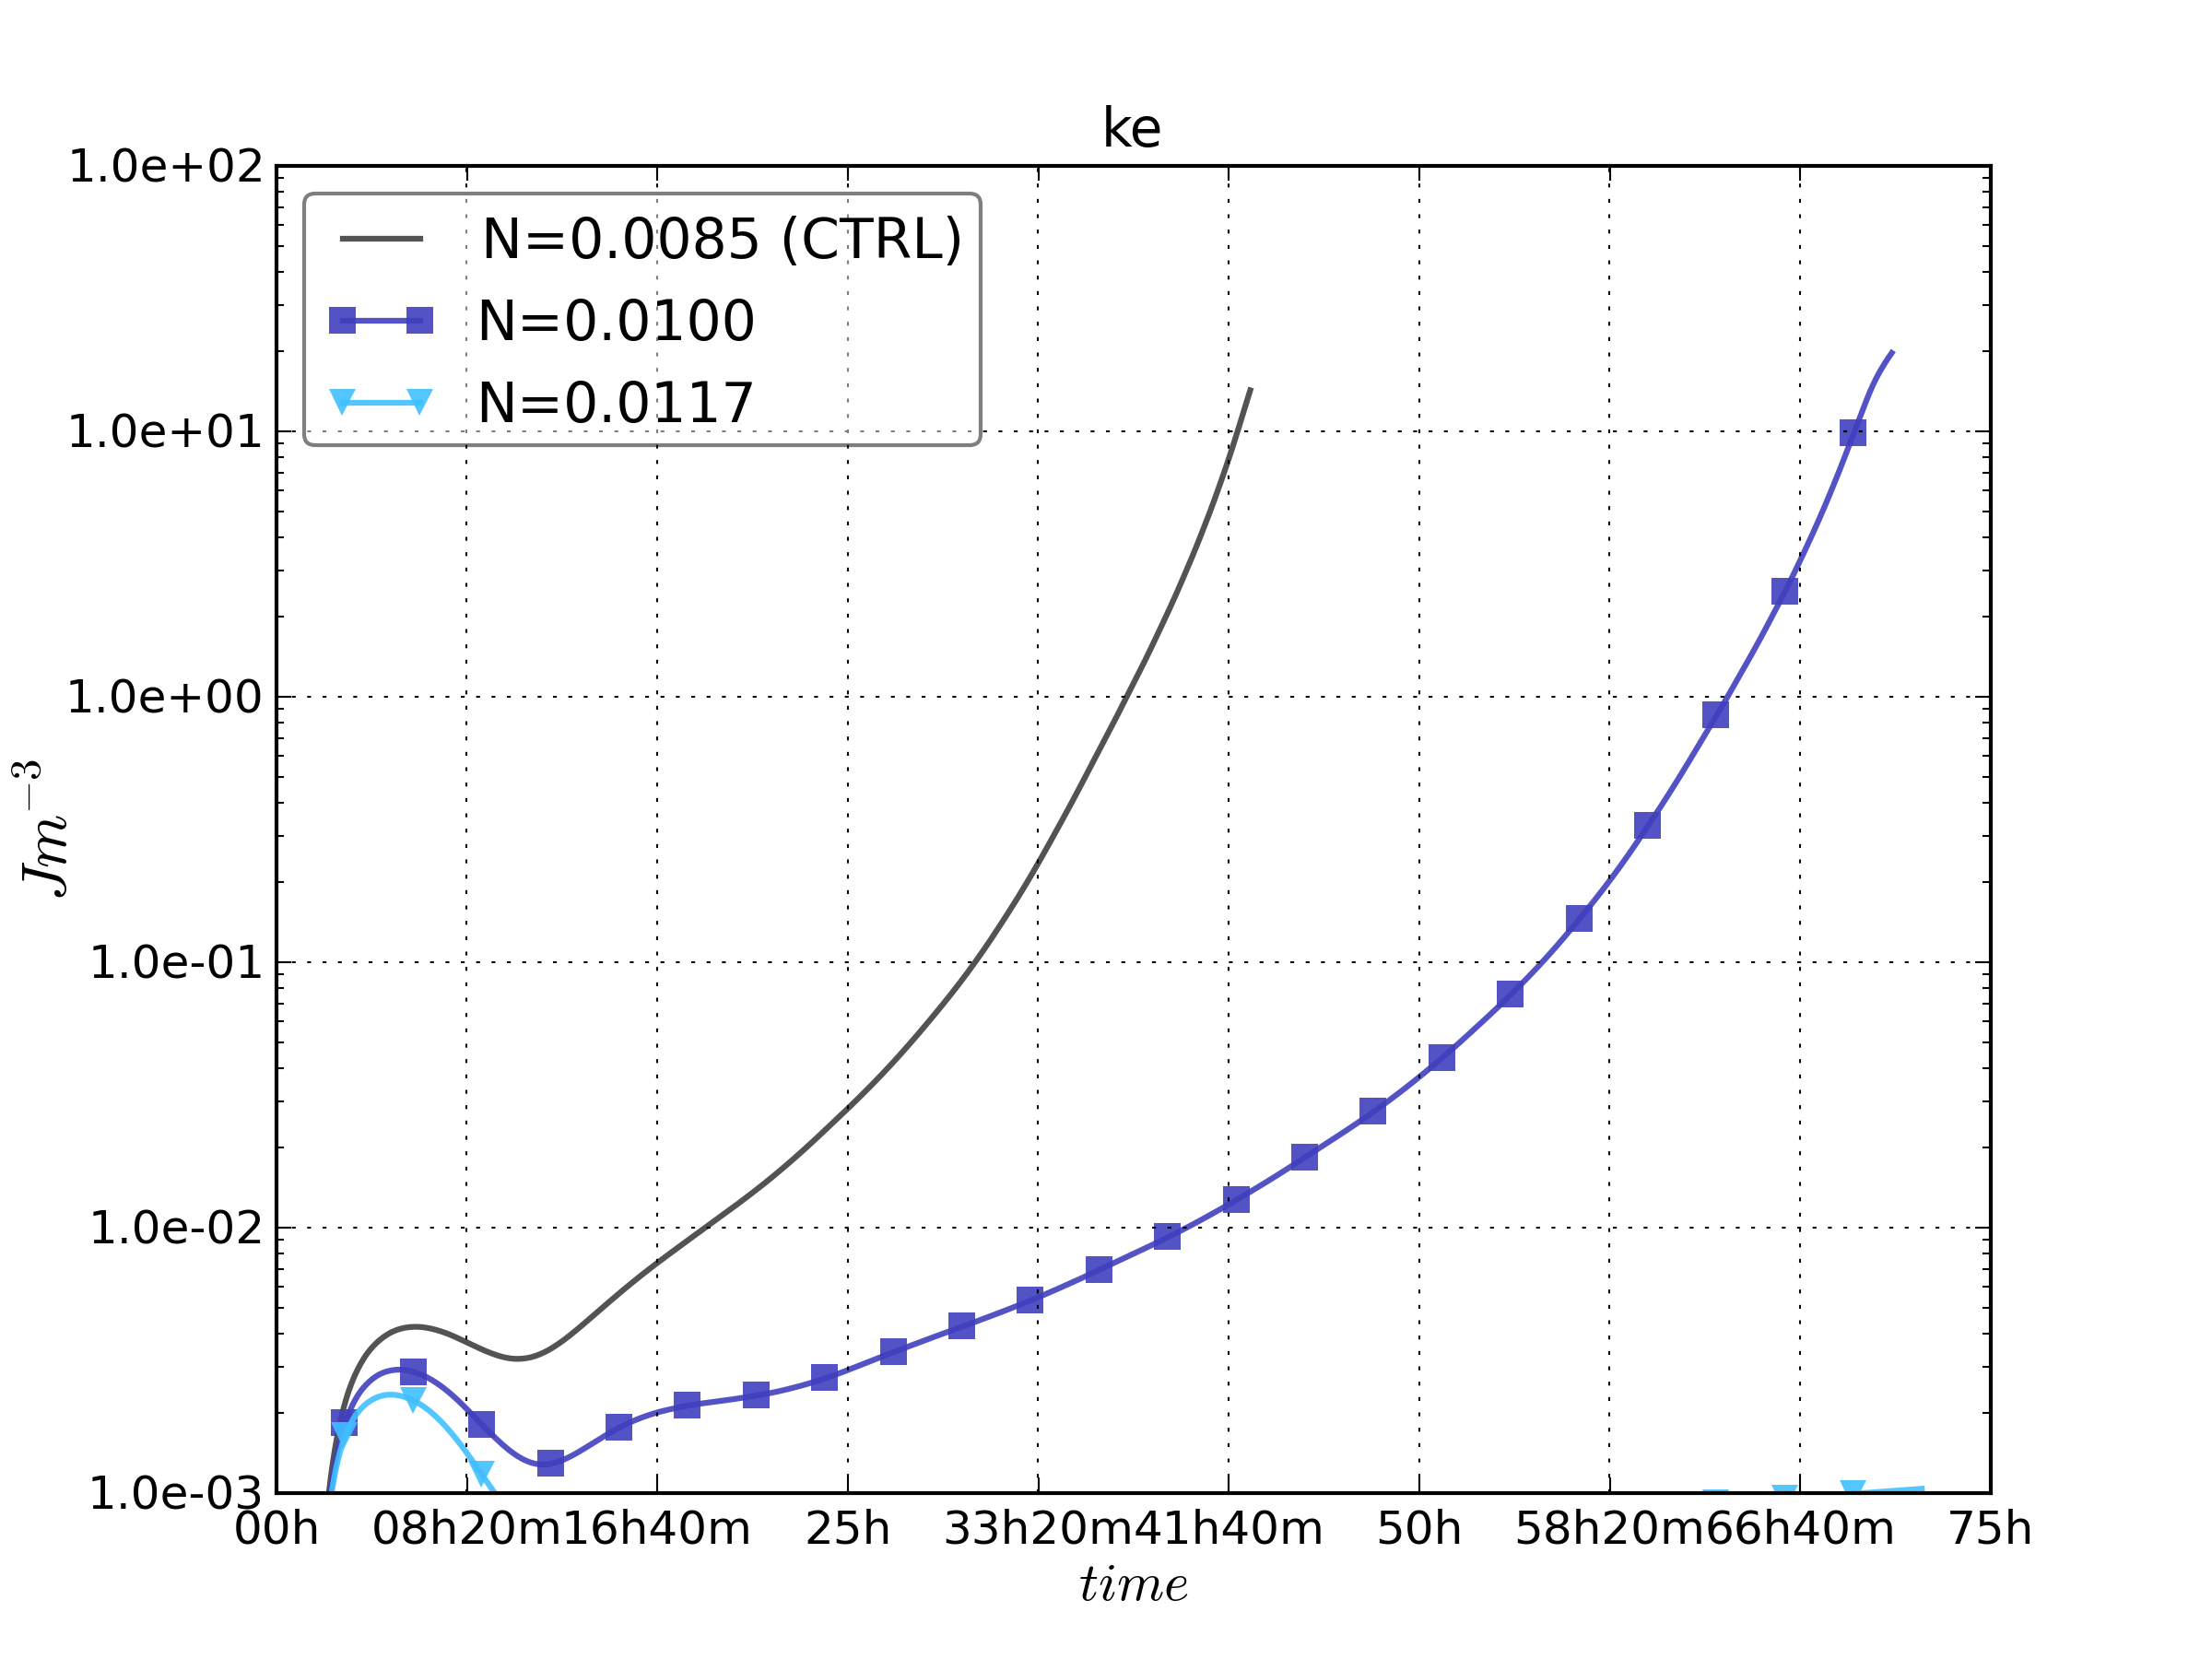
\includegraphics[width=\linewidth]{{./chapters/figures_results/ke.00h-72h.highN}.png}
%		\caption{ }
%        \label{fig:highN_ke}
%	\end{subfigure}
%	\hfill
%	\begin{subfigure}{0.45\textwidth}
%		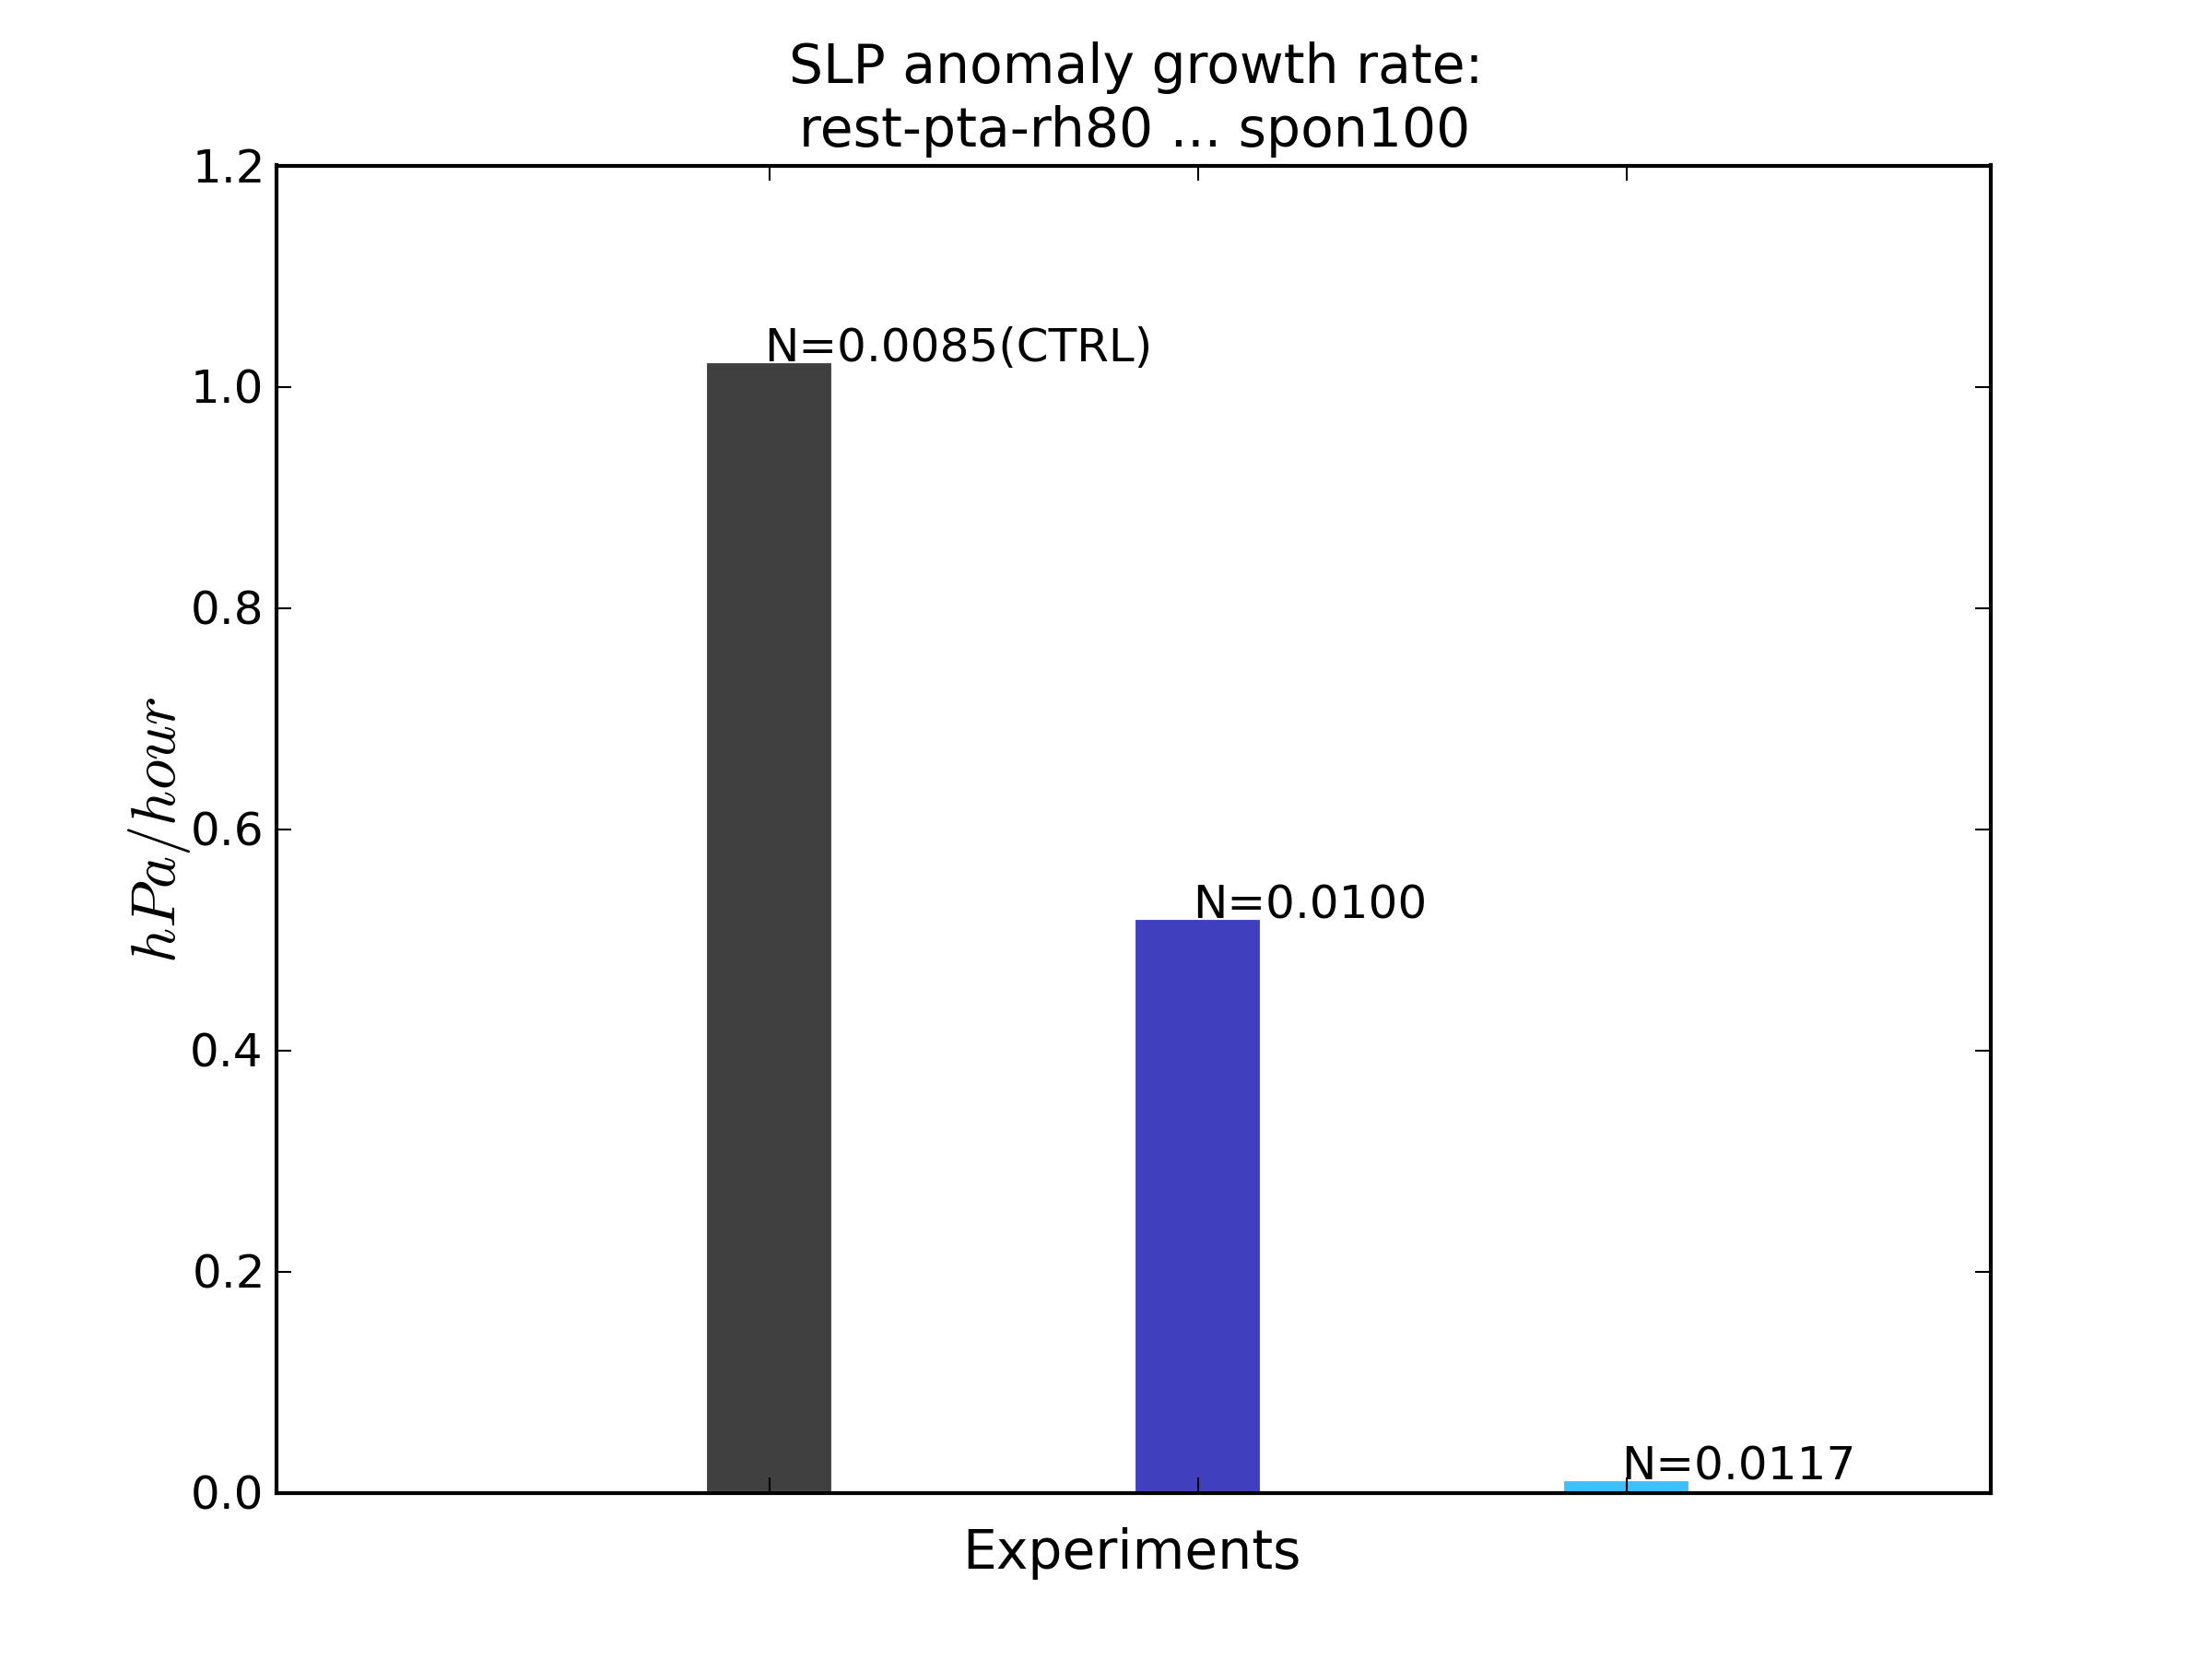
\includegraphics[width=\linewidth]{{./chapters/figures_results/slp_min_rate.00h-73h.highN}.png}
%		\caption{ }
%		\label{fig:highN_slp_rate}
%	\end{subfigure}
%        \caption{Эксперименты с пониженной устойчивостью фоновой атмосферы: изменение во времени кинетической энергии (слева) и чувствительность вихря к $N$ (справа).}
%\end{figure}
%
%На рис. \ref{fig:lowN_ke} представлена эволюция КЭ для экспериментов с пониженной статической устойчивостью относительно CTRL. Чтобы продлить время жизни вихря в этой группе экспериментов был уменьшен температурный контраст между воздухом и поверхностью воды за счет задания более высокой температуры атмосферы: $T_a=271\K$. Из-за этого развитие мезоциклона является более умеренным, чем в контрольном эксперименте, и кинетическая энергия даже в самом неустойчивом эксперименте лишь немного превышает $1\Jpm$. Более того, на основании рис. \ref{fig:lowN_ke} можно сказать, что стратификация $N\approx 0.0040\pers$ близка к критической для развития температурной аномалии: при $N>0.0040\pers$ рост КЭ не наблюдается. С точки зрения падения давления в центре вихря чувствительность интенсивности вихря к статической устойчивости показана на рис. \ref{fig:lowN_slp_rate}.
%
%Случай повышенной статической устойчивости рассматривается на примере экспериментов, в которых вертикальный градиент температуры равнялся $3\Kpkm$ ($N=0.0100\pers$) и $4\Kpkm$ ($N=0.0117\pers$). Рост КЭ в условиях более устойчивой стратификации ожидаемо оказывается слабее, чем в контрольном эксперименте, хотя после перемешивания нижних слоев атмосферы скорость роста в $N=0.0100\pers$  становится сравнима с контрольным. Сопоставление КЭ в трех экспериментов (рис. \ref{fig:highN_ke}) также обнаруживает наличие порогового значения для развития вихря. Таким образом, при разности температуры воды и воздуха $32\K$ (CTRL) и при градиенте температуры большем, чем $3\Kpkm$, выбранная амплитуда аномалии в 'сухой' атмосфере недостаточна для развития мощного мезоциклона.
%
%\subsection{Влияние устойчивости атмосферы на структуру атмосферных движений}
%Снижение статической устойчивости атмосферы отразилось не только на интегральных характеристиках, представленных выше, но и на пространственной динамике циклонической аномалии. Уже в первые часы модельного времени после инициализации температурного возмущения при разном $N$ волны, связанные с геострофическим (градиентным) приспособлением, имеют тем больше амплитуду и тем меньше фазовую скорость, чем меньше устойчивость. В этом можно убедиться на примере колебаний вертикальной скорости  $\tilde{w}$ в конкретной точке области (рис. \ref{fig:lowN_wfluct}).
%
%\begin{wrapfigure}{L}{0.5\textwidth}
%\begin{center}
%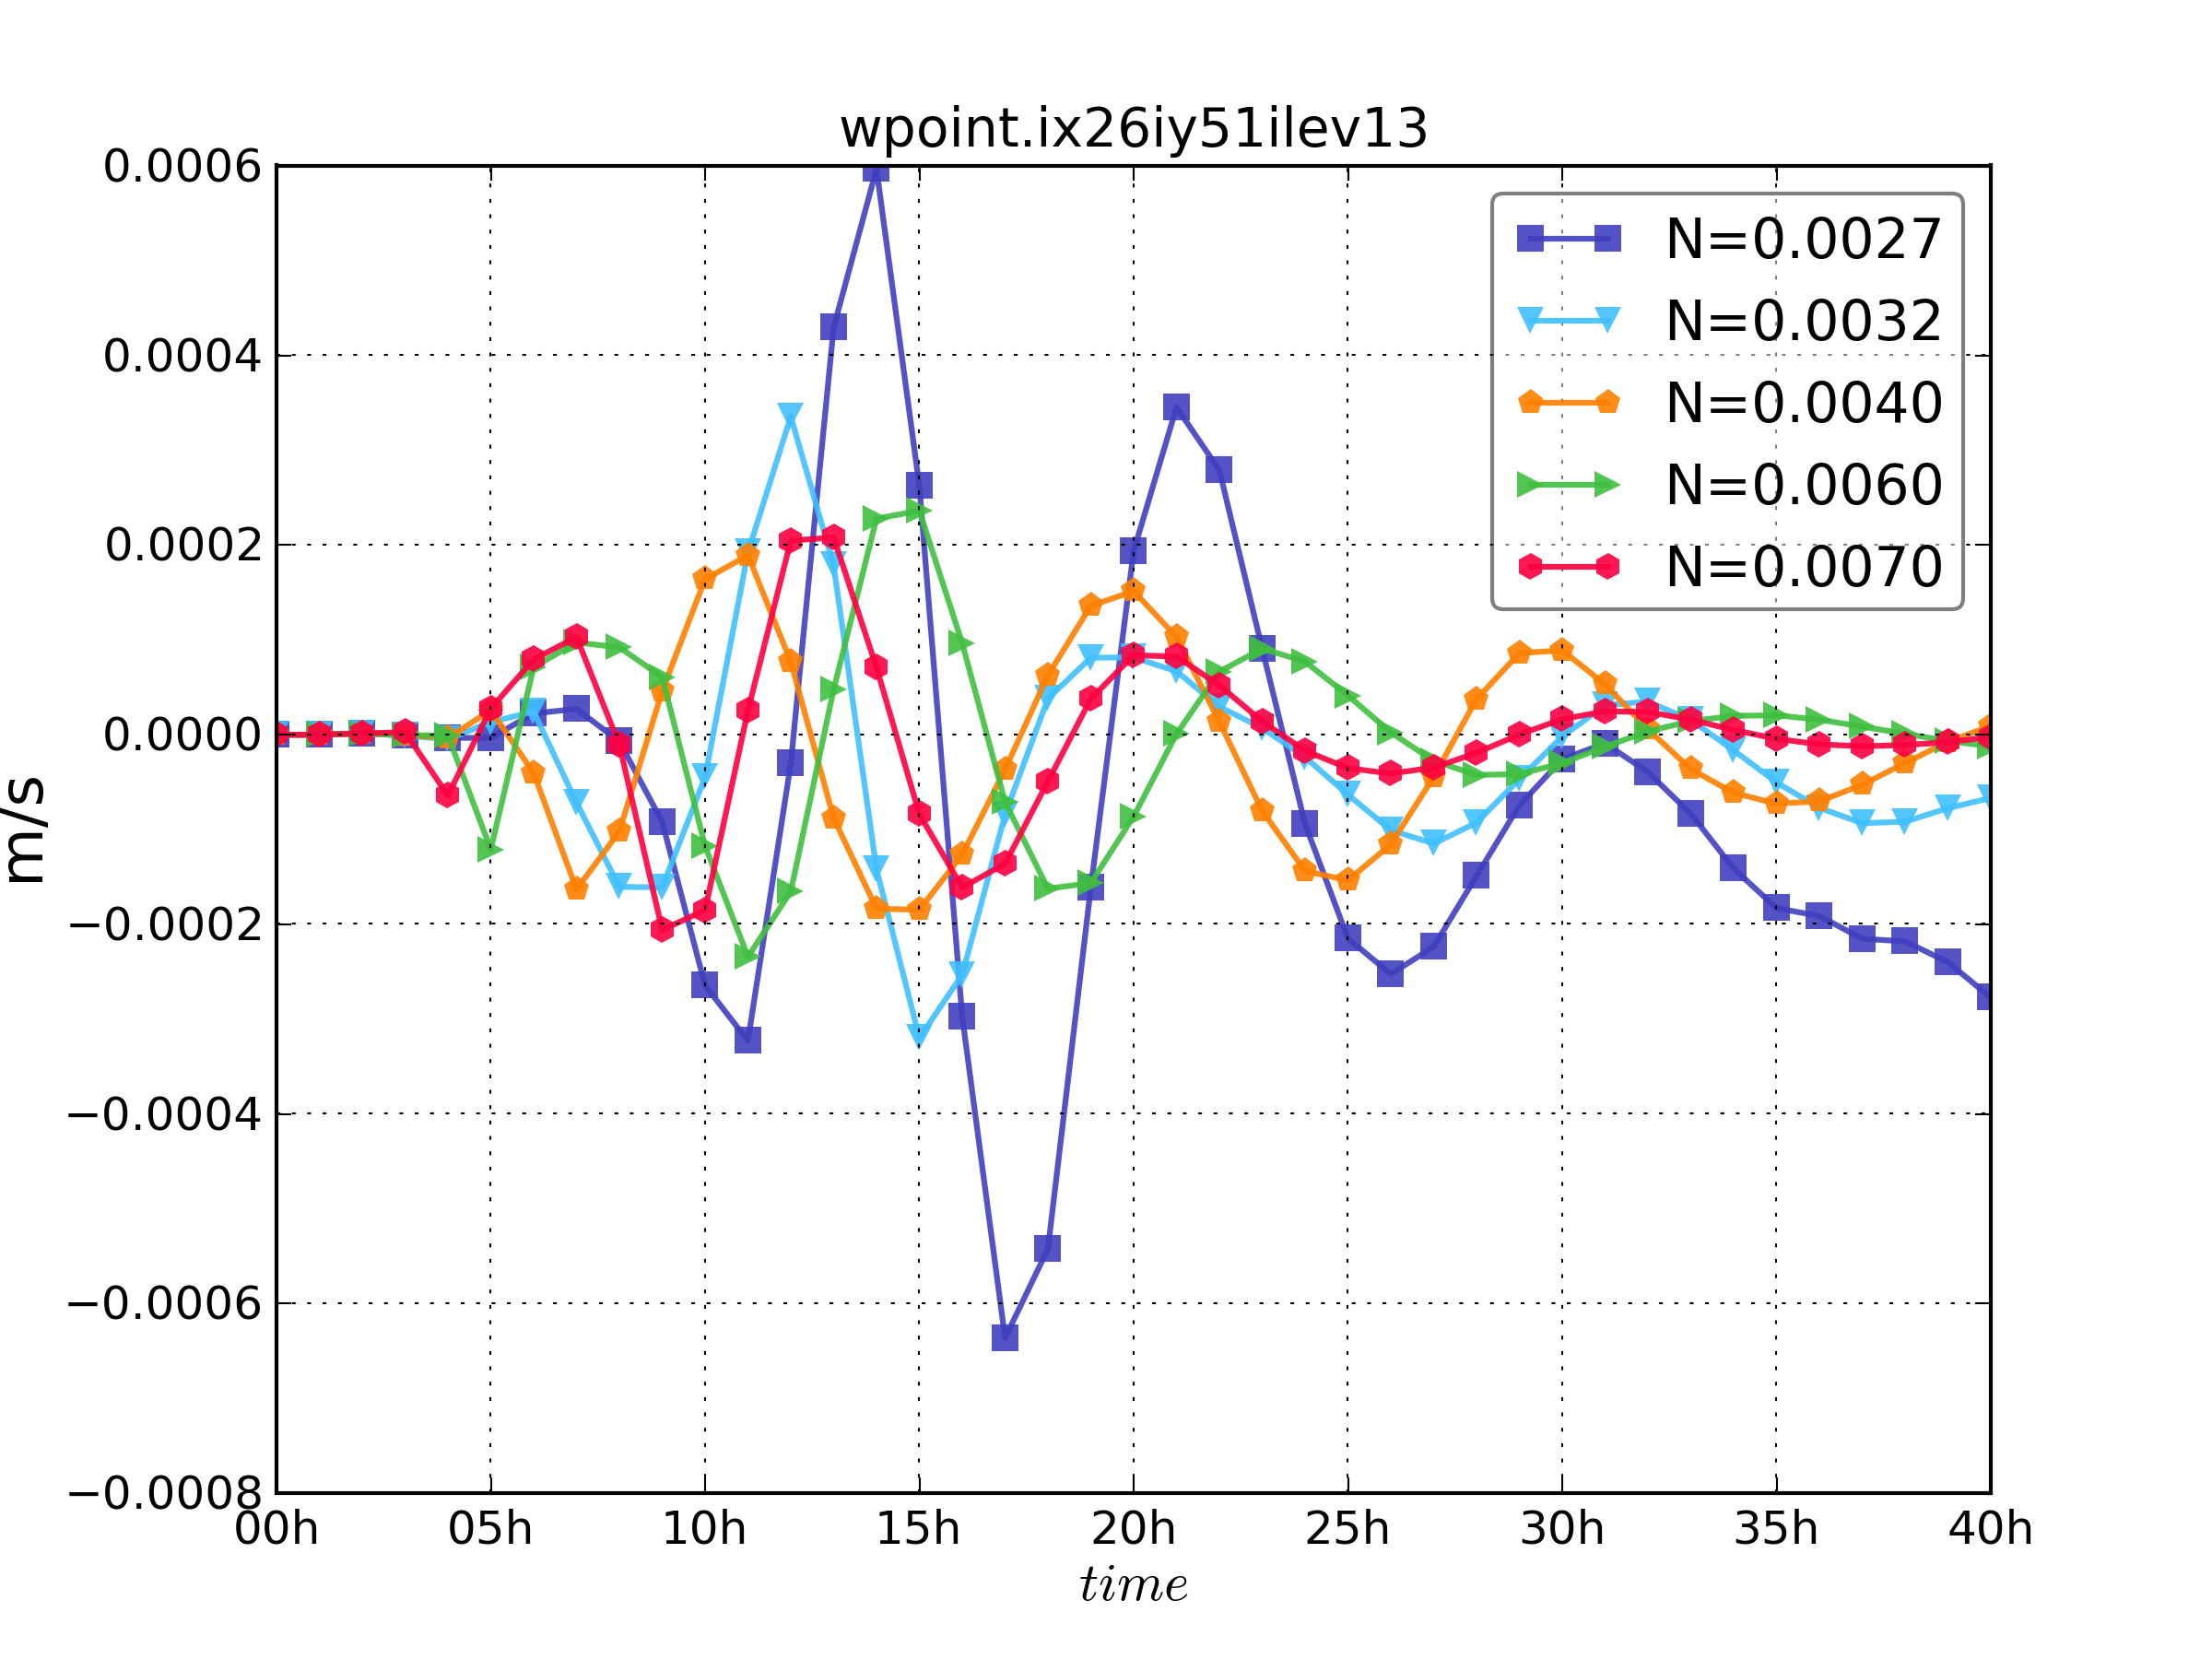
\includegraphics[width=\linewidth]{{./chapters/figures_results/wpoint.ix26iy51ilev13.00h-39h.stability}.png}
%\end{center}
%\caption{Колебания вертикальной скорости в точке ($r=250\km,p=300\hpa$) в экспериментах с разной фоновой стратификацией атмосферы.}
%\label{fig:lowN_wfluct}
%\end{wrapfigure}
%
%Горизонтальные разрезы вертикальной скорости показывают, что в экспериментах с самой низкой устойчивостью амплитуда инерционно-гравитационных волн на одном расстоянии от центра распределена не равномерно, а имеет четыре максимума, ориентированные к углам расчетной области. Данное обстоятельство говорит о неодинаковом поглощении излучаемых волн в буферной зоне модели и приводит к тому, в определенный момент четырехполюсная структура начинает преобладать, разделяя вихрь на четыре симметричные части, которые продолжают интенсифицироваться \ref{fig:lowN_hwind_split}. Напомним, что при повышенной устойчивости атмосферы в контрольном эксперимене вихрь разделялся на две части. Таким образом, при пониженной устойчивости (в данном случае при $N < 0.0060\pers$) развитие мезоциклона неустойчивым, а также становится более выгодно на мелких горизонтальных масштабах $L$.
%
%\begin{wrapfigure}{L}{0.5\textwidth}
%\begin{center}
%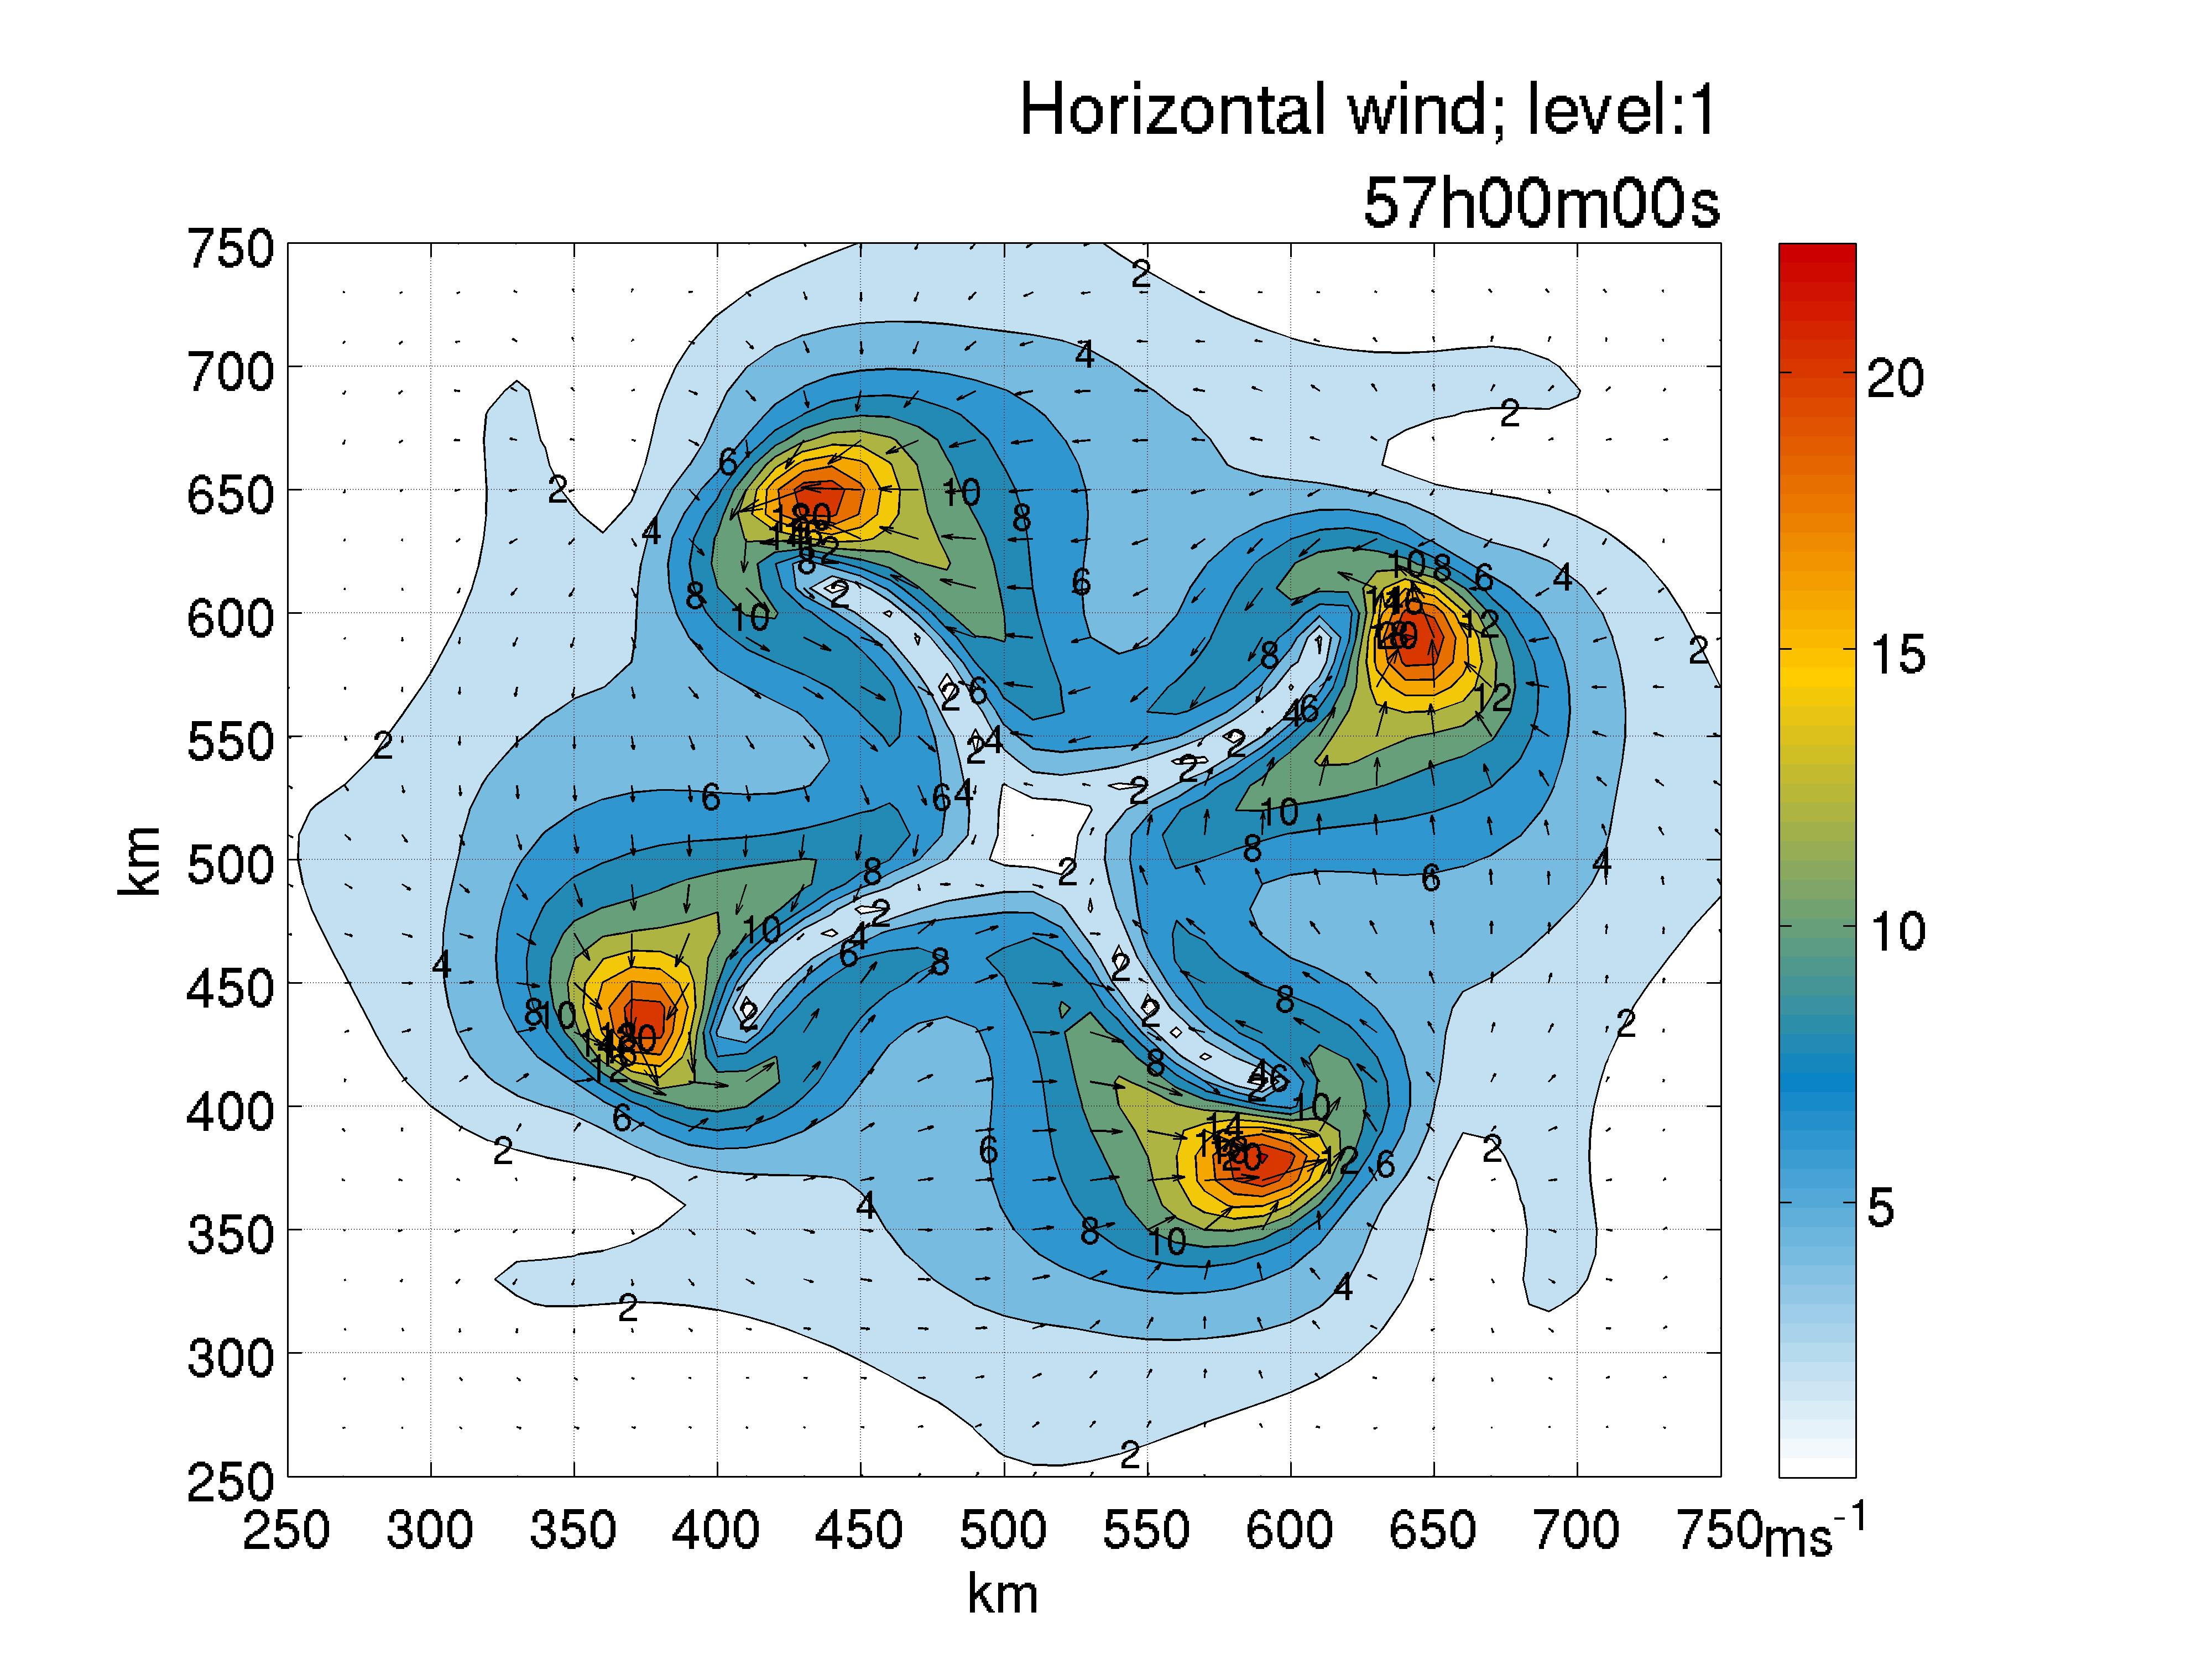
\includegraphics[width=\linewidth]{{./chapters/figures_results/VectorWind_p.x26-x76.y26-y76.ilev01.570000_lowN}.jpg}
%\end{center}
%\caption{Поле горизонтальной скорости ветра (область $500\times 500\km$). Эксперимент при $N=0.0027\pers$. 57 час модельного времени.}
%\label{fig:lowN_hwind_split}
%\end{wrapfigure}
%
%\section{Серия с разной температурой воды и воздуха}
%Выше были рассмотрена зависимость динамики вихря от таких характеристик фонового состояния атмосферы, как относительная влажность и статическая устойчивость. В них температура приводного слоя атмосферы равнялась $251\K$, а температура водной поверхности составляла $283\K$, создавая значительный вертикальный градиент температуры между водой и воздухом. В реальной атмосфере настолько большой градиент температуры достигается нечасто \citep{ForbesLottes1985}, поэтому были поставлены эксперименты, в которых разность температуры $\Delta T$ меняется от $12$ до $29\K$ за счет увеличения температуры всей толщи атмосферы или уменьшения температуры поверхности океана. 
%
%Если проанализировать эволюцию кинетической энергии (\ref{}) для экспериментов с одной и той же ТПО ($283\K$), но разной температурой атмосферы, то можно увидеть, что величина и скорость роста кинетической энергии пропорциональна разнице температур на границе вода-воздух, причем данная зависимость нелинейная: при малых значениях $\Delta T$ отличия между экспериментами менее заметны. Этот факт подтверждается зависимостью интенсивности циклона от $\Delta T$ и соответствующей таблицей \ref{}, в которой управляющим параметром чувствительности является $\Delta T$.
%
%Теперь вместо температуры воды зафиксируем параметр $\Delta T$, а температуру воздуха и воды изменим и опять же обратимся к ходу кинетической энергии на рис. \ref{} и \ref{}. На первом из этих рисунков сравнивается несколько экспериментов с $\Delta T=20\K$, на втором разность составляет $\Delta T=26\K$. Хорошо видно, что кривые на каждом из графиков почти не отличаются друг от друга. Из этого следует интуитивно понятный вывод, что динамика полярных мезоциклонов гораздо больше зависит от разности температур поверхности и атмосферы, чем от температуры поверхности самой по себе (в отличие от тропических циклонов \citep{EmanuelRotunno1989}). Схожие оценочные эксперименты проводились авторами \citep{YanaseNiino2007}, и ими было выяснено что чувтствительность вихря к средней температуре воды и воздуха (при фиксированной разнице) также невелика. Однако в экспериментах в указанной статье чувствительность к температуре обнаруживает зависимость от степени бароклинности атмосферы: чем меньше сдвиг ветра, тем больше чувствительность. По-видимому, это связано с тем, что при увеличении бароклинности фоновой атмосферы в бюджете кинетической энергии растет доля бароклинного слагаемого (аналогичного $C(A,K)$), а роль остальных факторов уменьшается.
%
%\section{Потоки тепла с поверхности}
%Многие особенности развивающегося вихря, описанные в предыдущих разделах, указывают на то, что в его динамике наиболее велика роль процессов при взаимодействии с подстилающей поверхностью, а именно турбулентных потоков явного и скрытого тепла. 
%
%В настоящем разделе подводятся результаты нескольких серий экспериментов, в которых потоки тепла и импульса с поверхности были отключены или искусственно изменены. Как уже было сказано в пункте \ref{sec:exp:surfpar}, эти эксперименты позволят с уверенностью говорить о роли потоков с поверхности в динамике вихря, а также о том, какой механизм доминирует в эволюции вихря.
%
%\subsection{Эксперименты без потоков явного и скрытого тепла в приводном слое}
%\label{sec:res:nohle}
%
%
%\begin{figure}[h]
%	\centering
%	\begin{subfigure}{0.45\textwidth}
%		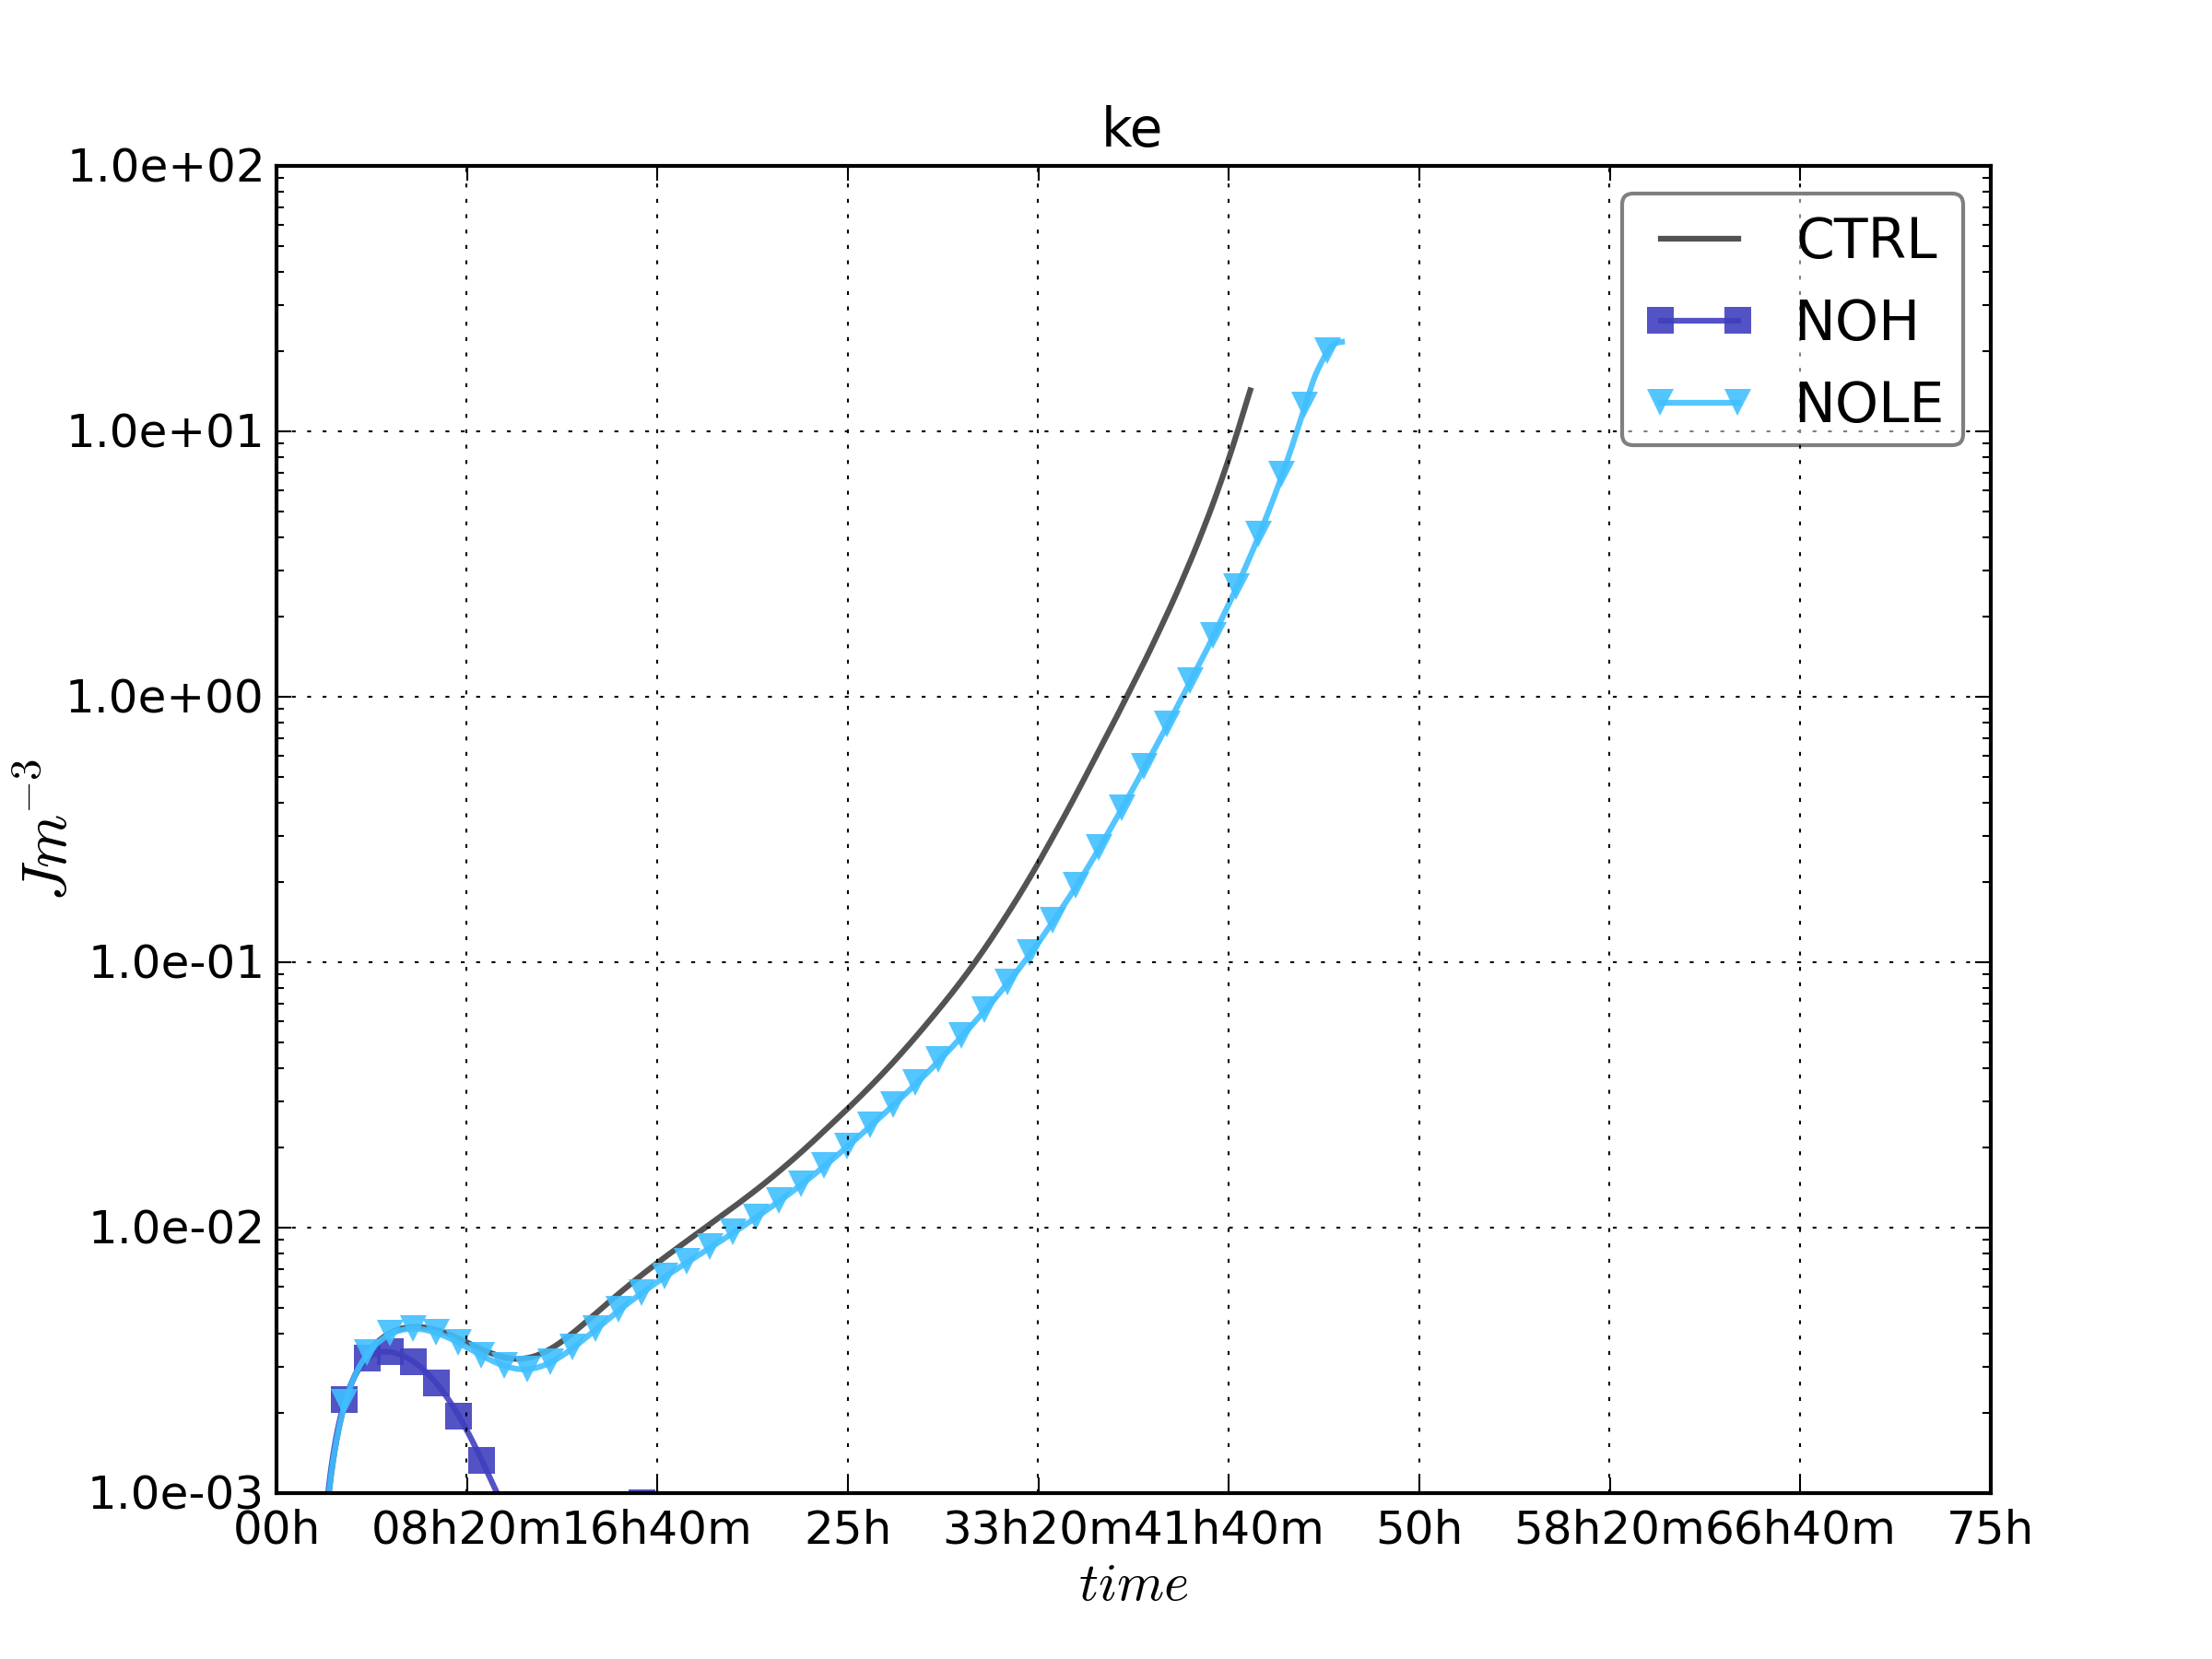
\includegraphics[width=\linewidth]{{./chapters/figures_results/ke.00h-72h.nohle}.png}
%		\caption{ }
%        \label{fig:nohle_ke}
%	\end{subfigure}
%	\hfill
%	\begin{subfigure}{0.45\textwidth}
%		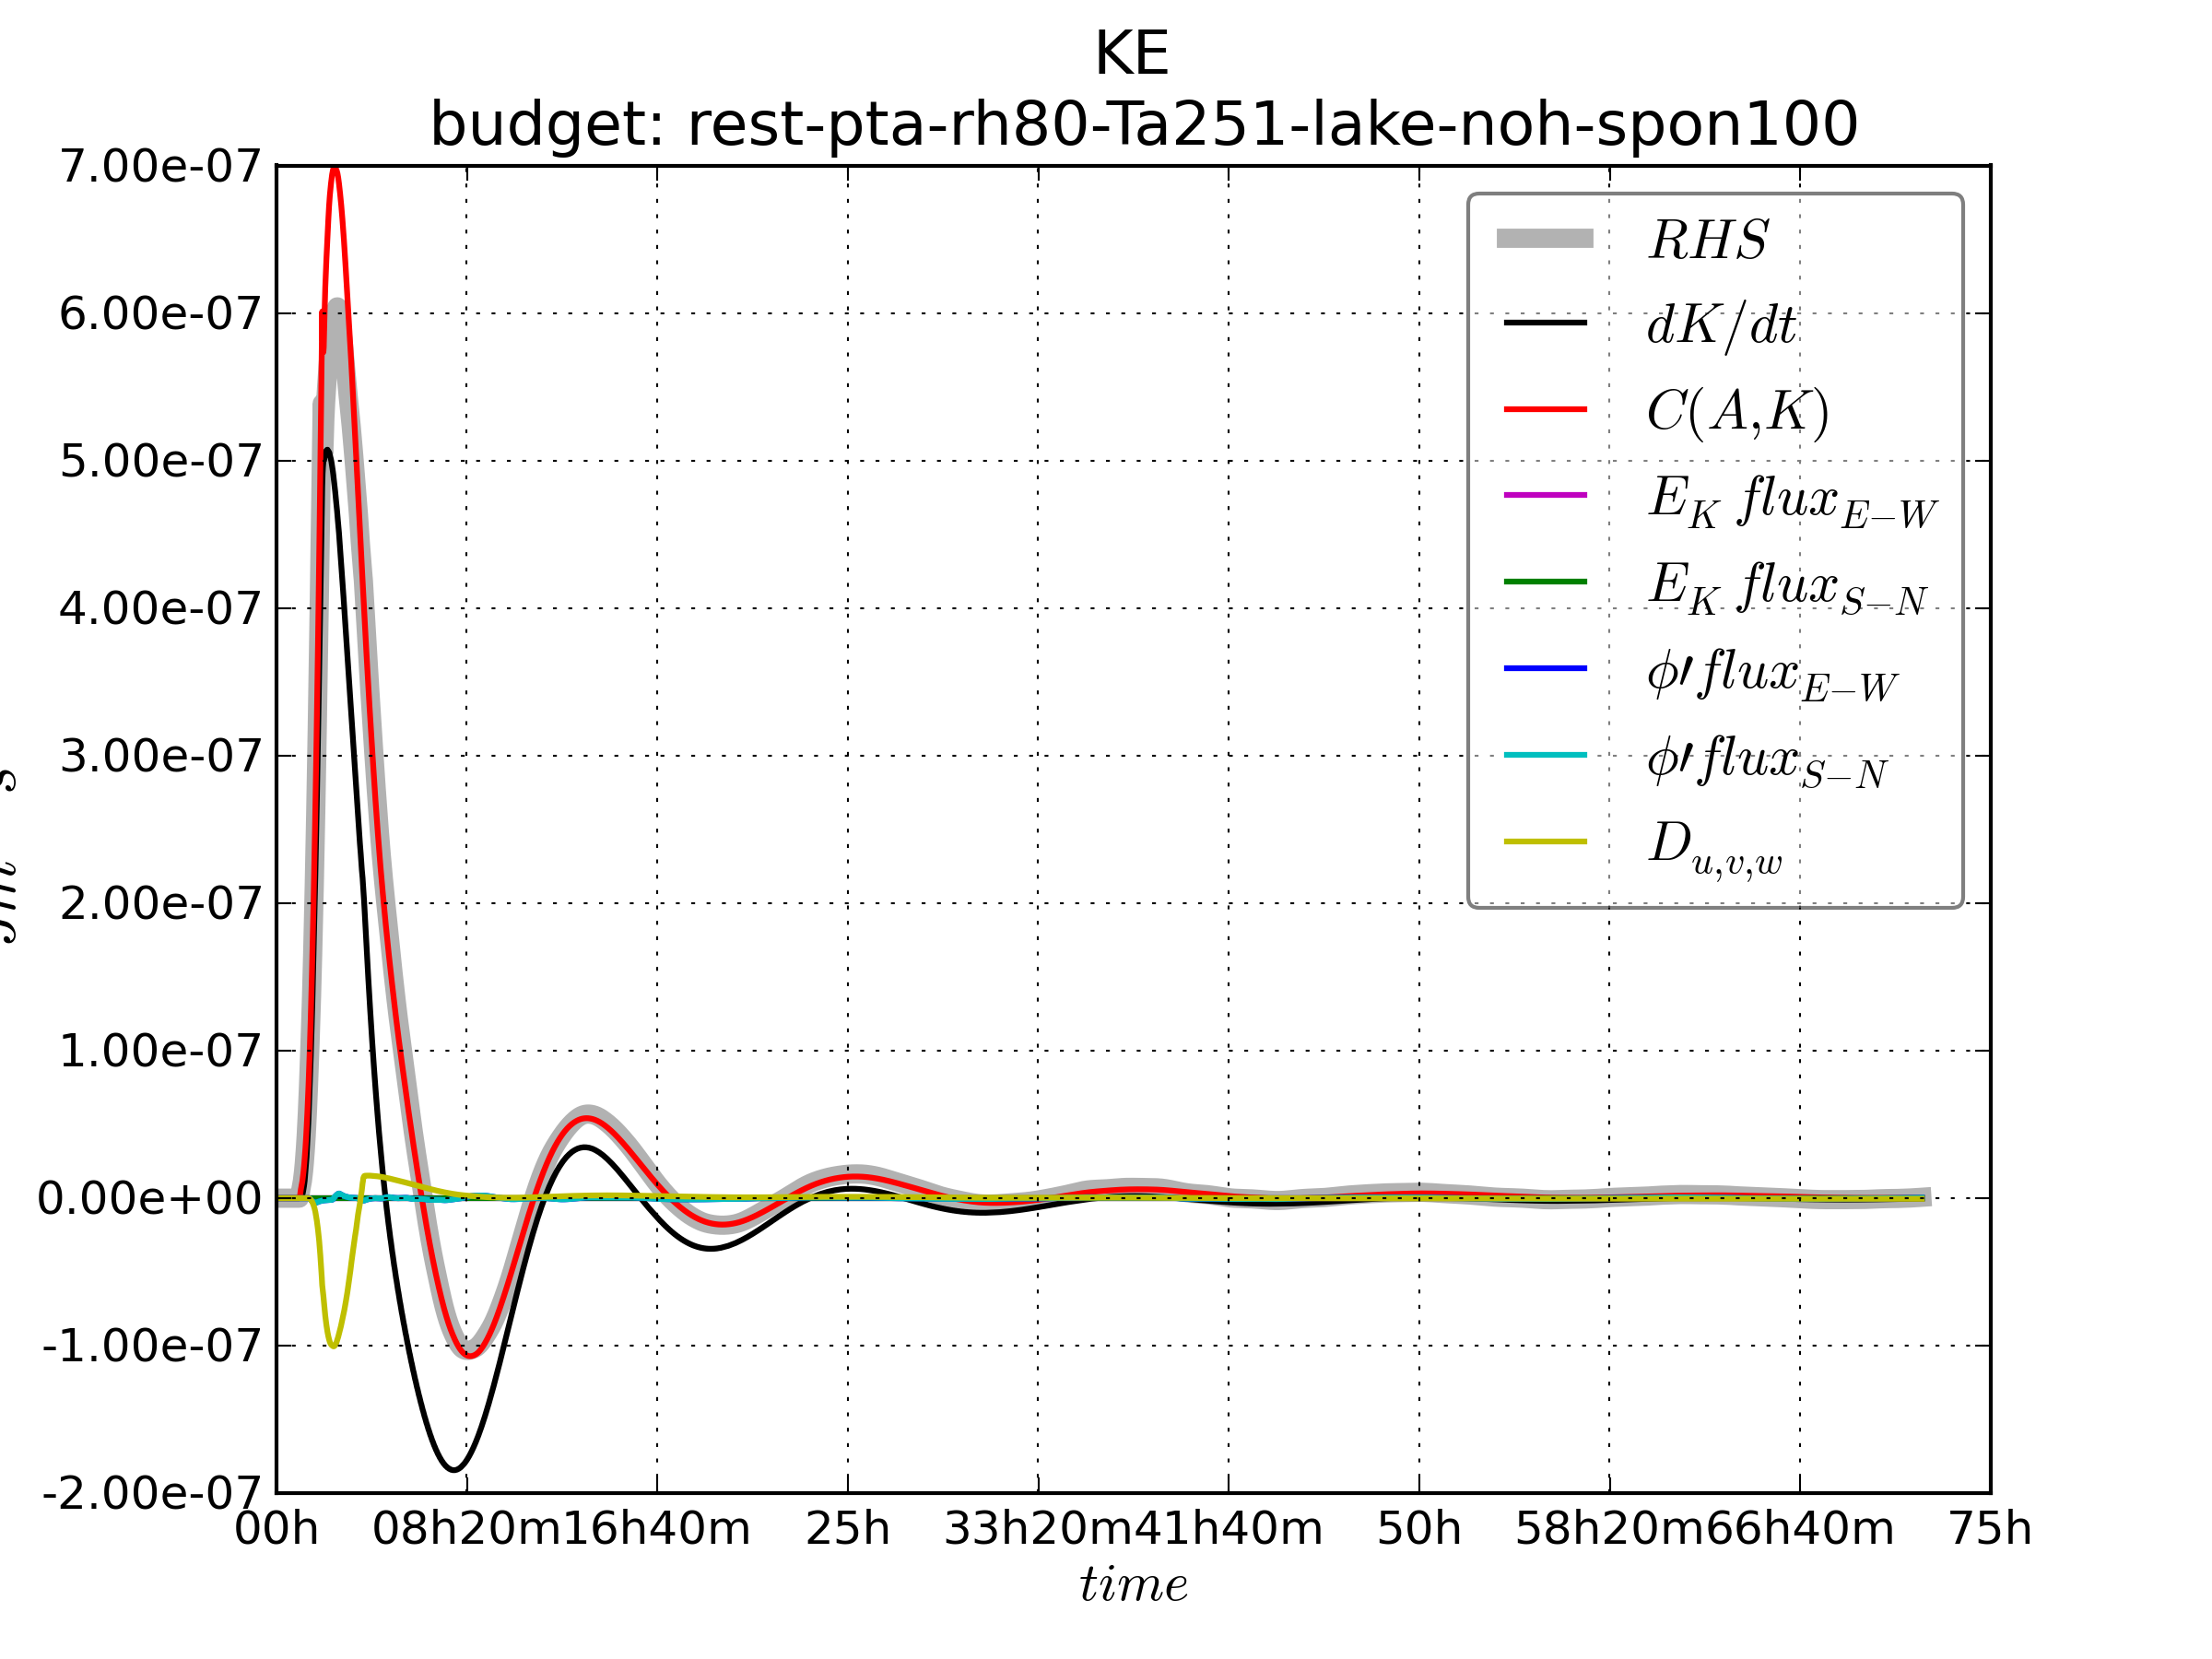
\includegraphics[width=\linewidth]{{./chapters/figures_results/rest-pta-rh80-Ta251-lake-noh-spon100.dkdt}.png}
%		\caption{ }
%		\label{fig:noh_dkdt}
%	\end{subfigure}
%        \caption{Эволюция кинетической энергии в экспериментах с отключенными потоками тепла (NOH) и влаги (NOLE) в приводном слое по сравнению с контрольным экспериментом (слева) и бюджет кинетической энергии в эксперименте NOH (справа).}
%\end{figure}
%
%Как будет развиваться начальная температурная аномалия в чисто адиабатической атмосфере --- без притока тепла от фазовых переходов воды и без турбулентных потоков с поверхности? Резонно предположить, что для интенсификации вихря их будет не хватать, особенно это касается потоков тепла с поверхности. Убедиться в этом можно по результатам экспериментов NOH, NOLE, NOHLE, в которых в модели были отключены соответственно потоки явного или скрытого тепла и оба потока одновременно. Представленная на рис. \ref{fig:nohle_ke} эволюция кинетической энергии мало отличается в эксперименте NOLE. В эксперименте NOH после возникновения перехода части ДПЭ (запасенной в начальной аномалии) в КЭ и формирования слабой циклонической циркуляции, рост кинетической энергии постепенно прекращается \ref{fig:noh_dkdt}. Заметим, что полностью вихрь не исчезает (согласуется с теорией, изложенной в \citep{RT2003}), а КЭ остается на уровне $10^{-4}\Jpm$. 
%
%\subsection{Эксперименты с разными параметризациями потоков тепла}
%\begin{wrapfigure}{r}{0.5\textwidth}
%\begin{center}
%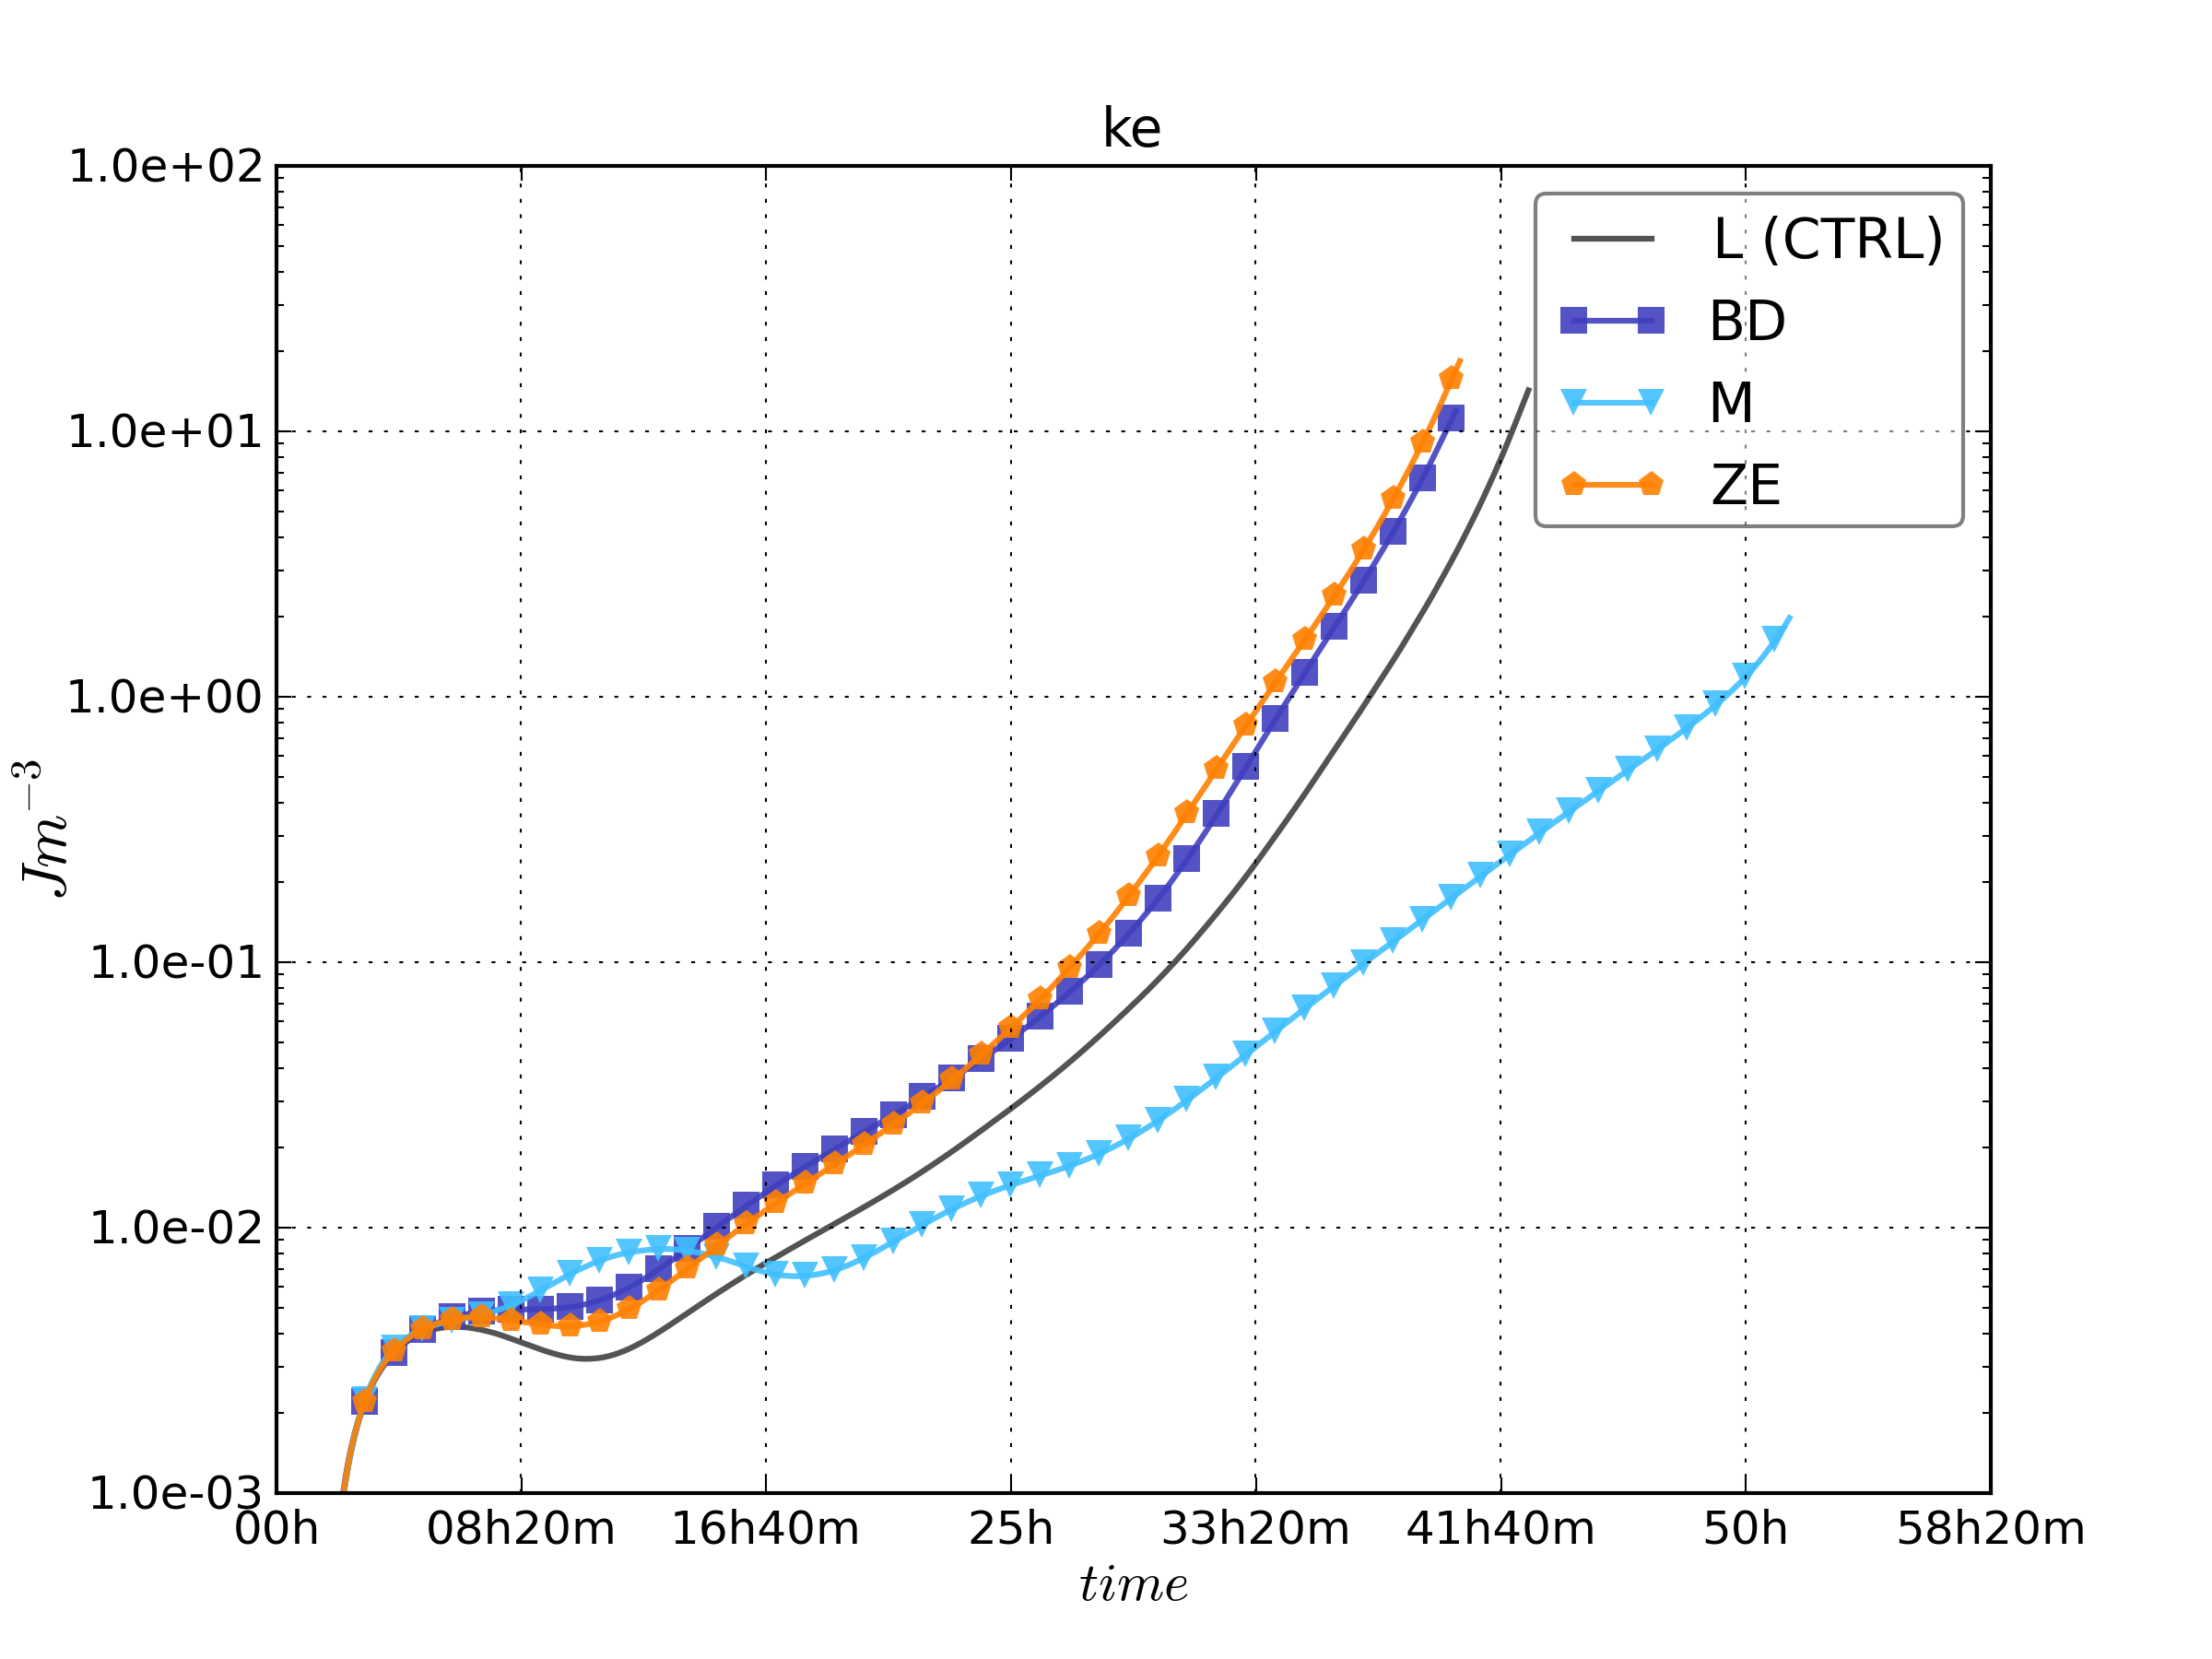
\includegraphics[width=\linewidth]{{./chapters/figures_results/ke.00h-51h30m.surfpar}.png}
%\end{center}
%\caption{Эволюция кинетической энергии в экспериментах с параметризациями BD, M, ZE турбулентных потоков в приводном слое по сравнению с контрольным экспериментом (L)}
%\label{fig:surfpar_ke}
%\end{wrapfigure}
%Начнем с того, что сравним результаты расчетов, сделанных с использованием разных параметризаций для турбулентных потоков в приземном слое. Их краткое описание и принятые обозначения представлено в главе \ref{sec:exp:surfpar}. В контрольном эксперименте использовалась параметризация L \citep{Louis1979}.
%
%Изменения кинетической энергии в модели \ref{fig:surfpar_ke} схожи между собой для экспериментов L, BD и ZE, но существенно отличаются для эксперимента с параметризацией M: в последнем темпы роста кинетической энергии меньше, и с середины первых суток значения КЭ отличаются на порядок или даже на 2 порядка. Тем не менее, вихрь во всех четырех экспериментах интенсифицируется до больших скоростей.
%При анализе бюджета ДПЭ было выявлено, что в конце каждого эксперимента происходят колебания с растущей амплитудой ипериодом (4--8 минут). Такие флуктуации прослеживаются только в слагаемом диффузии, в остальных они крайне малы. В самой ДПЭ, которая в конце экспериментов растет медленно, это не проявляется, как и на динамике остальных энергетических характеристик. Ранее других они возникают в эксперименте ZE, но схожи по характеру с таковыми в L и BD. Что касается эксперимента M, то на полученном отрезке эксперимента таких флуктуаций не выявлено.
%
%\begin{wrapfigure}{L}{0.5\textwidth}
%\centering
%\vspace{-30pt}
%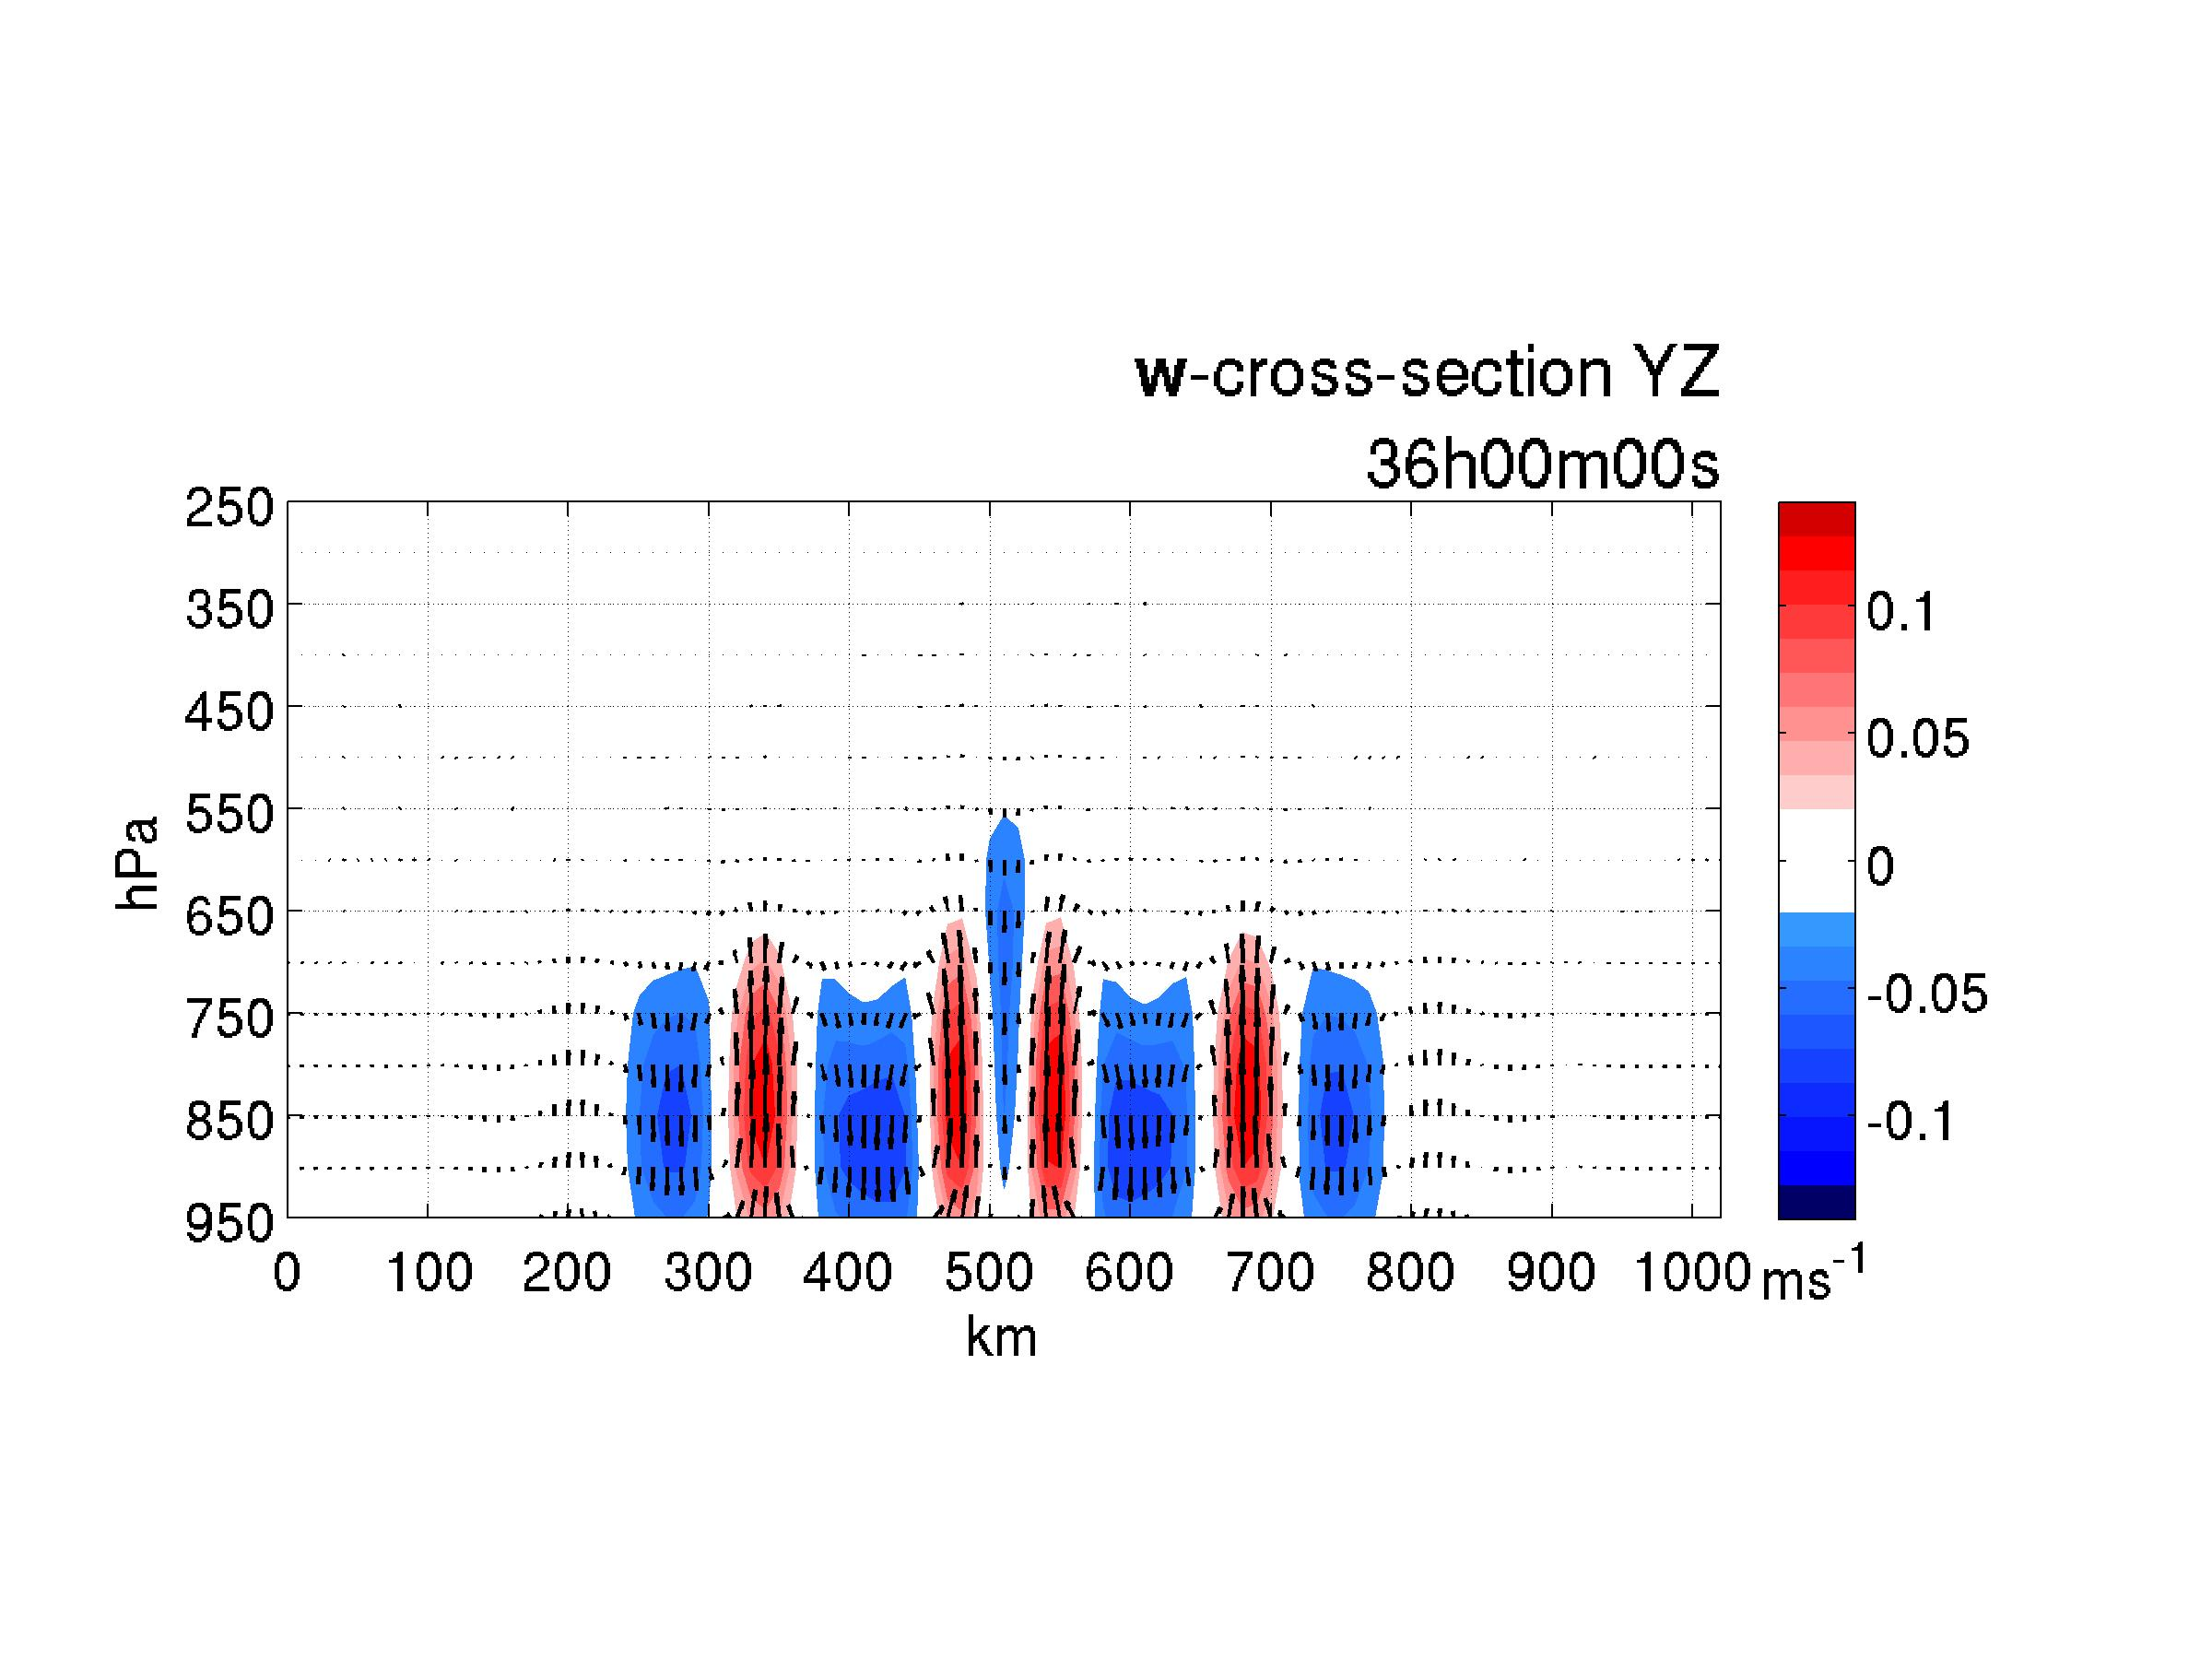
\includegraphics[width=\linewidth]{{./chapters/figures_results/W_cross_p.ix52.360000.FLAKE}.jpg}
%\vspace{-40pt}
%\caption{Зональный вертикальный разрез поля $w$-компоненты скорости (контуры) и значений вектора скорости (стрелки) в эксперименте M (36 ч.).}
%\label{fig:flake_wcross}
%\end{wrapfigure}
%
%Выявленные энергетической диагностикой различия между экспериментом M и остальными тремя экспериментами существуют из-за неодинакового воспроизведения конвекции в той или иной параметризации: параметризация M позволяет развитие свободной конвекции. Другими словами, в параметризациях потоков тепла по-разному заложена зависимость потока энергии с подстилающей поверхности от скорости ветра: при одинаковых скоростях приводного ветра поток явного тепла на радиусе максимального ветра в мезоциклоне отличается более, чем в 3 раза. Более того, в эксперименте M интерференция инерционно-гравитацинных волн порождает возникновение отдельных максимумов давления на периферии циклонического возмущения, что в дальнейшем приводит к распространению ячейковой конвекции во всей расчетной области. Размер отдельных конвективных ячеек (кроме центрального вихря) составляет $\approx 80\km$ в диаметре и $3500\m$ по вертикали (рис. \ref{fig:flake_wcross}).
%В качестве промежуточного вывода можно отметить, что использование параметризации Миронова (эксперимент M) дает более устойчивый мезоциклон и менее 'взрывной' его рост в конце эксперимента. По-видимому, различия в экспериментах сгладятся при условии, что атмосферные условия будут включать ненулевой фоновый поток. Сходство результатов в экспериментах L И BD дает право использовать параметризацию Бусингера-Дайера в дополнительных экспериментах \ref{sec:res:wishe}
%
%\subsection{CISK/WISHE для сухого (контрольного) и влажного эксперимента}
%\label{sec:res:wishe}
%Рассматриваемое циклоническое возмущение, очевидно, можно отнести к типу полярных мезоциклонов конвективного генезиса (энергия бароклинной или баротропной неустойчивости  здесь отсутствует). В разделе \ref{} были описаны две основные концепции роста полярного мезоциклона в результате термической неустойчивости --- CISK и WISHE. Глубже понять природу вихря и выявить, какой из этих механизмов интенсификации вихря доминирует в наших экспериментах, позволяет методика, хорошо описанная в \citep{CraigGray1996}. В обеих концепциях скорость роста циклона зависит от процессов в пограничном слое атмосфере: от потоков тепла и влаги в WISHE и от конвергенции в CISK. Определить, какой механизм доминирует в динамике циклона можно, варьируя параметры подстилающей поверхности: шероховатость в CISK и доступное количество тепла в WISHE. То есть ключевой момент методики заключается в том, что трение на поверхности изменяется независимо от турбулентных потоков явного и скрытого тепла. В численной модели это достигается изменением коэффициентов турбулентного сопротивления ($C_D$) и тепло- и влагообмена ($C_H$).
%
%Тесты на чувствительность вихря к коэффициентам турбулентного обмена проводились как для 'сухих' экспериментов (DRY), так и для 'влажных' (MOIST). На рис. \ref{} представлена КЭ для серии экспериментов, в которых $C_H$ уменьшался или увеличивался на $20$ и $50\%$. Большой разброс в полученных кривых указывает на сильную зависимость роста циклона от доступного тепла в приземном слое атмосферы: так, в экспериментах DRY значения КЭ отличаются более чем на порядок при изменении коэффициента на $50\%$. Несколько меньшую чувствительность обнаруживается в серии MOIST.
%
%Что касается влияния силы трения и конвергенции в центре вихря, то их роль незначительна (рис. \ref{}). Более того, повышение коэффициента сопротивления $C_D$ приводит лишь к увеличению стока КЭ, замедляя рост вихря, что не компенсируется более интенсивной экмановской подкачкой, особенно в экспериментах DRY. Систематического увеличения удельной влажности в пограничном слое атмосферы при увеличении $C_H$, необходимого в теории CISK Чарни и Элиассена, также не было выявлено.
%
%Чувствительность динамики вихря к потокам с поверхности можно оценить и с точки зрения углубления барической депрессии в центре. Интенсивность, определенная таким образом (см. \ref{}), в наглядно показана для $C_H$  на диаграмме \ref{}, а для $C_D$  на диаграмме \ref{}.
%
%Полученные результаты еще раз подтверждают, что циклоническое возмущение развивается благодаря взаимодействию океана и атмосферы по принципам теории WISHE. Вклад эффектов условной неустойчивости второго рода незначителен: область конвекции в вихре \emph{в центре} существует только в первые 18 часов, перемещаясь затем по направлению от центра вихря. Если бы влияние конвергенции и потока влаги в верхние слои было бы велико, то эффект изменения коэффициентов турбулентного обмена проявился бы в начале экспериментов.
%
%Результаты проведенных экспериментов качественно соответствуют результатам расчетов по осесимметричной модели \citep{CraigGray1996, EmanuelRotunno1989}. В отличие от указанной работы, тенденция к усилению вихря при увеличении коэффициента турбулентного обмена для тепла и влаги сохраняется даже при предельных значениях этого коэффициента (хотя и в меньшей степени в экспериментах MOIST). Стоит отметить, что для более уверенных результатов необходимо также рассмотреть динамику CAPE в районе развития вихря. В то же время в некоторых работах было установлено, что небольшое количество CAPE также может существовать при доминировании WISHE, также как, и при CISK-циклоне она тоже необязательно бывает большой. Кроме того, необходимо провести аналогичные серии экспериментов для других параметризаций потоков тепла и импульса.
%
%\section{Параметризация подсеточного перемешивания}
%Результат: в случае С-Л в КПС создается заметный 
%градиент пот. температуры, в случае же нелокального замыкания КПС 
%почти полностью перемешан и распространяется выше. Эксперимент
%с вихрем (но без потока $10\mps$) показывает, что вихрь затухает, не дотигнув и скорости $3\mps$. Это при фоновой стратификации $2\Kpkm$. При этом затухание выглядит, как увеличение размеров вихря с одновременным падением максимальной скорости. В области ненулевых скоростей ветра (т.е. в области циркуляции вихря), где есть поток тепла с поверхности, быстро образуется полностью перемешанный КПС. Думаю, теперь можно усилить факторы неустойчивости вихря (включить конденсацию, например), чтобы он развивался посильнее. В аналогичном эксперименте с замыканием С-Л вихрь развивается до $\approx 50\mps$, и превышается число Куранта.
%
%\subsection{Замыкание Смагоринского-Лилли (разный коэффициент турбулентности)}
%
%\subsection{Противоградиентное нелокальное замыкание}
%
%\subsection{Чувствительность к размерам температурной аномалии}
%Корректное моделирование полярных мезоциклонов в исследовательских или оперативных целях зависит не только от представления в модели фонового состояния атмосферы, но и от правильного задания параметров циклонического возмущения. Последнее можно показать на примере проведенной серии экспериментов, в которой варьировались радиус, высота и амплитуда температурной аномалии при ее инициализации \ref{}. Эволюция кинетической энергии в соответствующих экспериментах показана на рис.\ref{}--\ref{}, которые говорят о том, что эффект от изменения размеров или же амплитуды термического возмущения неодинаков. Оценивая результаты с точки зрения относительных изменениях $\theta_{max}$, $H$, $r_{out}$ на можно утверждать о низкой чувствительности вихря к высоте аномалии, средней чувствительности к горизонтальным размерам и сильной чувствительности к начальной температуре в центре. Так, при начальном максимуме температурного возмущения в $10\K$ продолжительность устойчивого эксперимента составила 1.5 сут., а при $\theta_{max}=2\K$ циклоническое возмущение не достигло значительной скорости и за трое суток.
%
%Такие же выводы можно сделать, сравнив изменение минимального давления \ref{}. Как и в описанных выше сериях экспериментов, построим зависимость интенсивности вихря от амплитуды начальной аномалии. Результаты количественной оценки чувствительности представлены в табл. \ref{}. 
%
%\section{Серия с разной скоростью фонового потока}
%В серии экспериментов, описываемых в данном подразделе, выясняется влияние фоновой скорости ветра на динамику циклонической аномалии. Как было сказано в \ref{sec:expplan:flow}, фоновый поток имеет строго зональное направление и однороден по пространству, а его скорость равна от $2$ до $10\mps$. При этом вихрь инициализировался на западе области.
%
%Все эксперименты качественно очень похожи друг на друга, отличаясь лишь скоростью роста КЭ \ref{} и временем достижения мезоциклоном боковых граней области, близи которых структура нарушается. На указанном рисунке видно, что КЭ рассматриваемых экспериментов ненулевая, так как это полная кинетическая энергия, включающая и средний поток. Рост КЭ начинает ускоряться в конце первых суток интегрирования, однако значения $dK/dt$ меньше, чем в контрольном эксперименте. С другой стороны, интенсивный рост циклонического возмущения начинается тем раньше, чем больше скорость начального (фонового) ветра. По-видимому, причиной такого соотношения является взаимосвязь циркуляции приводного ветра и потока явного тепла с поверхности: в эксперименте с сильным внешним воздушным потоком значения $H$ велики уже в первые часы существования циклонического возмущения (достигая $\approx 500\Wpermsq$).
%
%В бюджете КЭ среди слагаемых правой части преобладает $C(A,K)$, как и в контрольном эксперименте, но постепенно возрастает отрицательный вклад адвективных слагаемых, ответственных за поток энергии через боковые грани расчетной области \ref{}.
%Таким образом, процесс генерации ДПЭ и перехода ее в КЭ в данной серии экспериментов качественно не отличается от контрольного эксперимента. Это закономерно, так как начальное поле ветра не имеет градиентов скорости, а значит, фоновая атмосфера не является дополнительным резервуаром ДПЭ для атмосферных возмущений. Однако вклад фонового потока меняет структуру полярного мезоциклона. Скорость адвекции вихря оказывается приблизительно в 1.5 раза больше, чем фоновая скорость потока. Из-за этого с тыльной стороны циклона возникает своеобразный шлейф из волн, напоминающих волны обтекания орографического препятствия, а сам циклон приобретает форму запятой (рис. \ref{}). Кроме того, разделение циклонического возмущения на два мелких возмущения происходит более явно. Момент разделения отражается на эволюции полной КЭ в виде короткого плоского участка.
%
%%\begin{wrapfigure}{L}{0.5\textwidth}
%%\begin{center}
%%\includegraphics[width=\linewidth]{{./chapters/figures_results/ctrl_fields/pt_dev_z.x26-x76.y26-y76.ilev01.020000_}.jpg}
%%\end{center}
%%\caption{Поле отклонений температуры ($\theta'$) при инициализации возмущения (2 ч. модельного времени)}
%%\label{fig:initanom}
%%\end{wrapfigure}

\begin{thebibliography}{12}
 \bibitem{ER89}
Emanuel KA, Rotunno R. 1989. Polar lows as Arctic hurricanes. \textit{Tellus} \textbf{41A:} 1-17.
\end{thebibliography}

\end{document}